%!TEX ROOT = thesis.tex
\chapter{Results and Analysis}

\hspace{12.7mm}This chapter presents the results of the research work. The results are analyzed in detail to provide insights into the findings and their implications for the study. The chapter is organized into three main sections. Each section presents the related results that support the research objectives of developing cost-effective machine learning models to predict the risk of cognitive impairment and classify its etiology.

\section{Current Cognitive Status Classification Results}
This section presents the results for the first research objective, which focuses on developing cost-effective models to classify current cognitive status. The section provides results for the normal cognition (\acrshort{NC}) vs. cognitive impairment (\acrshort{CI}) prediction task and the cognitive impairment but not dementia (\acrshort{CIND}) vs. dementia prediction task.

\subsection{Feature Selection Results}

This subsection presents the results of the feature selection for the two classification tasks. The proposed feature selection method is based on the ensemble feature ranking methods and the automatic feature selection threshold using a class overlap measure. 

To evaluate this method, the results were compared with the baseline and the Boruta algorithm. The evaluation was performed using a random forest (\acrshort{RF}) model in internal cross-validation. The goal was to find a subset of features that reduces the data complexity and improves the computational efficiency while maintaining a high level of predictive performance. Several metrics were used to compare the methods. These include the number of selected features, the class overlap (Maximum Fisher's Discriminant Ratio (\acrshort{F1})), and the model's predictive performance measured using the geometric mean (\acrshort{G-mean}).

\subsubsection{Feature Selection Results for the NC vs. CI Classification Task}\label{sec:feature-selection-task1}

As shown in Table~\ref{table:fs-task1}, the proposed feature selection method successfully identified a minimal and cost-effective subset of features. The baseline model, which was based on the initial 68 features, achieved the highest predictive performance with a G-mean of 0.840. However, it had high data complexity (0.946 F1 feature overlap score) and lowest computational efficiency. The proposed method selected only 12 features. This is an 82\% reduction from the baseline and also fewer than the 15 features selected by the Boruta method. This minimal feature set had only a minor acceptable impact on predictive performance, achieving a G-mean of 0.829. This score is competitive with both the baseline and the Boruta method.

\begin{table}[!ht]
    \centering
    \caption{Comparison of feature selection methods for the NC vs. CI classification task}
    \begin{tabular}{|c|c|c|c|c|}
    \hline
        Method & Number of Features & G-mean & Fitness Score & F1 \\ \hline
        Baseline & 68 & 0.840 & 0.700 & 0.946 \\ \hline
        Boruta & 15 & 0.833 & 0.824 & 0.815 \\ \hline
        \textbf{Proposed Method} & \textbf{12} & \textbf{0.829} & \textbf{0.828} & \textbf{0.788} \\ \hline
        \multicolumn{5}{p{400pt}}{\footnotesize \hl{F1: Fisher's discriminant ratio (feature overlap measure), Fitness Score: combined score balancing performance and feature reduction, G-mean: geometric mean score.}}
    \end{tabular}
    \label{table:fs-task1}
\end{table}

More importantly, the subset of features selected by our method achieved the lowest F1 feature overlap score (0.788). This result indicates that our overlap-guided approach was the most successful in reducing data complexity and improving the separability of classes. This reduction in complexity and feature count translated directly into better efficiency. The model using our selected features had a training throughput of 20,870 samples per second. This is over 2.7 times faster than the baseline model and it also achieved the highest inference speed.

Finally, our proposed method achieved the highest fitness score (0.828), slightly exceeding the Boruta method (0.824), and significantly better than the baseline (0.700). This confirms that our method provided the best overall balance between high performance and model simplicity, which directly answers our research objective to develop a cost-effective solution.

The 12 features selected by the proposed method for the NC vs. CI task are presented in Table~\ref{table:features-task1}. The selected feature set is composed of four categories of accessible data. The majority of the selected features (8 out of 12 features) are assessments of instrumental activities of daily living (\acrshort{IADL}) collected using the Functional Activities Questionnaire (\acrshort{FAQ}). The remaining features include two demographic variables, a memory complaint from the Geriatric Depression Scale (\acrshort{GDS}), and an item from the Neuropsychiatric Inventory Questionnaire (\acrshort{NPI-Q}).

\begin{table}[h!]
\centering
\caption{List of selected features for the NC vs. CI Classification task}
\label{table:features-task1}
\begin{tabular}{ccc}
\toprule
\textbf{Feature Code} & \textbf{Feature Description} & \textbf{Feature Category} \\
\midrule
NACCAGE & Age & Demographics \\
SEX & Sex & Demographics \\
MEMPROB & Subject reported memory problem & GDS \\
BILLS & Pay bills and track spending & FAQ \\
TAXES & Assemble tax records & FAQ \\
SHOPPING & Shop alone for necessities & FAQ \\
GAMES & Play a game of skill & FAQ \\
EVENTS & Keep track of current events & FAQ \\
PAYATTN & Pay attention to a conversation & FAQ \\
REMDATES & Remember dates and appointments & FAQ \\
TRAVEL & Travel out of neighborhood & FAQ \\
ANX & Anxiety in the last month & NPI-Q \\
\bottomrule
\end{tabular}
\end{table}

\subsubsection{Feature Selection Results for the CIND vs. Dementia Classification Task}
Feature selection was also extended to the CIND vs. dementia classification task. The same comparative analysis was performed to evaluate the proposed method against a baseline and the Boruta method. The results of this comparison are illustrated in Table~\ref{table:fs-task2}.

\begin{table}[!ht]
    \centering
    \caption{Comparison of feature selection methods for the CIND vs. dementia classification task}
    \begin{tabular}{|c|c|c|c|c|}
    \hline
        Method & Number of Features & G-mean & Fitness Score & F1 \\ \hline
        Baseline & 71 & 0.833 & 0.694 & 0.941 \\ \hline
        Boruta & 14 & 0.799 & 0.800 & 0.889 \\ \hline
        \textbf{Proposed Method} & \textbf{11} & \textbf{0.815} & \textbf{0.820} & \textbf{0.754} \\ \hline
        \multicolumn{5}{p{400pt}}{\footnotesize \hl{F1: Fisher's discriminant ratio (feature overlap measure), Fitness Score: combined score balancing performance and feature reduction, G-mean: geometric mean score.}}
    \end{tabular}
    \label{table:fs-task2}
\end{table}

The proposed method selected a subset of 11 features. This represents an 84.5\% decrease from the 71 initial features used in the baseline and is also smaller than the 14 features selected by the Boruta method. In terms of the RF model performance, the baseline model had the highest G-mean score of 0.833. The proposed method obtained a G-mean of 0.815. This result was close to the baseline and was also considerably higher than the 0.799 G-mean from the Boruta method. The features selected by the proposed method balance high performance and reduced complexity, which is reflected by the highest fitness score. The fitness score of the proposed method (0.820) exceeded both the Boruta method (0.800) and the baseline (0.694).

The simplicity obtained by the proposed method can be observed in the feature overlap metrics. The proposed method achieved an F1 feature overlap score of 0.754, which was a significant improvement compared to both the Boruta method (0.889) and the baseline (0.941). Additionally, the high ratio of feature reduction resulted in an efficient model. The training process for the 11-feature model was over 2.7 times faster than training with the baseline features.

The 11 features that were selected by the proposed method for the CIND vs. dementia classification task are presented in Table~\ref{table:features-task2}. An analysis of the list shows that 8 out of 11 features are IADL features from the FAQ. The remaining features are primary language, energy scale, and appetite problems.

\begin{table}[h!]
\centering
\caption{List of selected features for the CIND vs. dementia Classification task}
\label{table:features-task2}
\begin{tabular}{ccc}
\toprule
\textbf{Feature Code} & \textbf{Feature Description} & \textbf{Feature Category} \\
\midrule
PRIMLANG & Subject's primary language & Demographics \\
BILLS & Pay bills and track spending & FAQ \\
TAXES & Assemble tax records & FAQ \\
SHOPPING & Shop alone for necessities & FAQ \\
GAMES & Play a game of skill & FAQ \\
MEALPREP & Prepare a balanced meal & FAQ \\ 
EVENTS & Keep track of current events & FAQ \\
REMDATES & Remember dates and appointments & FAQ \\
TRAVEL & Travel out of neighborhood & FAQ \\
ENERGY & Do you feel full of energy? & GDS \\
APP & Appetite and eating changes & NPI-Q \\
\bottomrule
\end{tabular}
\end{table}

The selected feature subset in this task can be compared to the one selected for the previous NC vs. CI task. The selected subsets share seven common FAQ features. However, the subset for the CIND vs. dementia classification task includes the ability to prepare a meal over the ability to pay attention to a conversation and includes different demographic, GDS, and NPI-Q features. More details of the selected features and their correlation results can be found in section \ref{sec:feature-selection-apdx} in the appendix.

\subsection{Data Resampling Results}
\label{sec:resampling_results}
This section presents the results of the data resampling method related to the first research objective. The objective is to develop an accurate classification model for the current cognitive status. These results demonstrate how the proposed data resampling methodology addresses class imbalance and class overlap. Handling these data complexities is important to develop an accurate, balanced, and generalizable model. The overlap-guided resampling methodology was applied to the two classification tasks to achieve this objective. The distribution of the target classes in the National Alzheimer's Coordinating Center (\acrshort{NACC}) Uniform Data Set (\acrshort{UDS}) and ADNI datasets is provided in Figure~\ref{fig:nacc-data-stat} and Figure~\ref{fig:adni-data-stat} in the appendix.

\subsubsection{Data Resampling Results for the NC vs. CI Classification Task}
\label{sec:resampling_nc_ci}
Based on the analysis of the data complexity, this task showed a slight class imbalance, with an imbalance ratio (\acrshort{IR}) of 1.452. A high degree of data complexity was also observed. The instance-level class overlap (\acrshort{kDN}) score was 0.209, and the structural class overlap (\acrshort{N1}) score was 0.304. The analysis of borderline examples revealed that around 32\% of the minority class (NC) instances were in the overlapped region. This is compared to only 15\% for the majority class (CI) instances. The measures indicated a high structural class overlap and a mild class imbalance. 

Based on these complexity measures, the ENN + \acrshort{KMeansSMOTE} hybrid resampling strategy was selected by the decision algorithm (Algorithm \ref{alg:data-resampling}). The Edited Nearest Neighbors (\acrshort{ENN}) method was applied first to clean noisy instances from both classes. Then, the K-means Synthetic Minority Over-sampling Technique (\acrshort{KMeansSMOTE}) was used. This method added synthetic examples to the safer and more sparse regions of the minority class. The effectiveness of this selected method was evaluated against the baseline (no data resampling) and standard data resampling techniques. The results are presented in Table~\ref{table:nc_ci_resampling} and are also visualized in Figure~\ref{figure:nc_ci_resampling_perf}.

\begin{table}[!ht]
    \centering
    \caption{Performance comparison of resampling methods for the NC vs. CI classification task using a random forest model}
    \begin{tabular}{|c|c|c|c|c|c|}
    \hline
        Method & G-mean & Recall (NC) & Recall (CI) & kDN & N1 \\  \hline
        Baseline & 0.829 & 0.860 & 0.799 & 0.209 & 0.294 \\ \hline
        ROS & \makecell{0.831 \\ {\small \hl{(p = 0.010)}}} & 0.885 & 0.781 & 0.213 & 0.293 \\ \hline
        RUS & \makecell{0.831 \\ {\small \hl{(p = 0.057)}}} & 0.\textbf{892} & 0.773 & 0.158 & 0.259 \\ \hline
        SMOTE & \makecell{0.831 \\ {\small \hl{(p = 0.004)}}} & 0.881 & 0.785 & 0.207 & 0.280 \\ \hline
        \makecell{\textbf{ENN +} \\ \textbf{KMeansSMOTE}} & \makecell{\textbf{0.832} \\ {\small \hl{(p = 0.026)}}} & 0.862 & \textbf{0.804} & \textbf{0.005} & \textbf{0.059} \\ \hline
        \multicolumn{6}{p{400pt}}{\footnotesize \hl{G-mean: geometric mean score, kDN: k-disagreeing neighbors (instance-level class overlap), N1: structural class overlap, Recall: per-class recall.}}
    \end{tabular}
    \label{table:nc_ci_resampling}
\end{table}

\begin{figure}[ht]
\centering
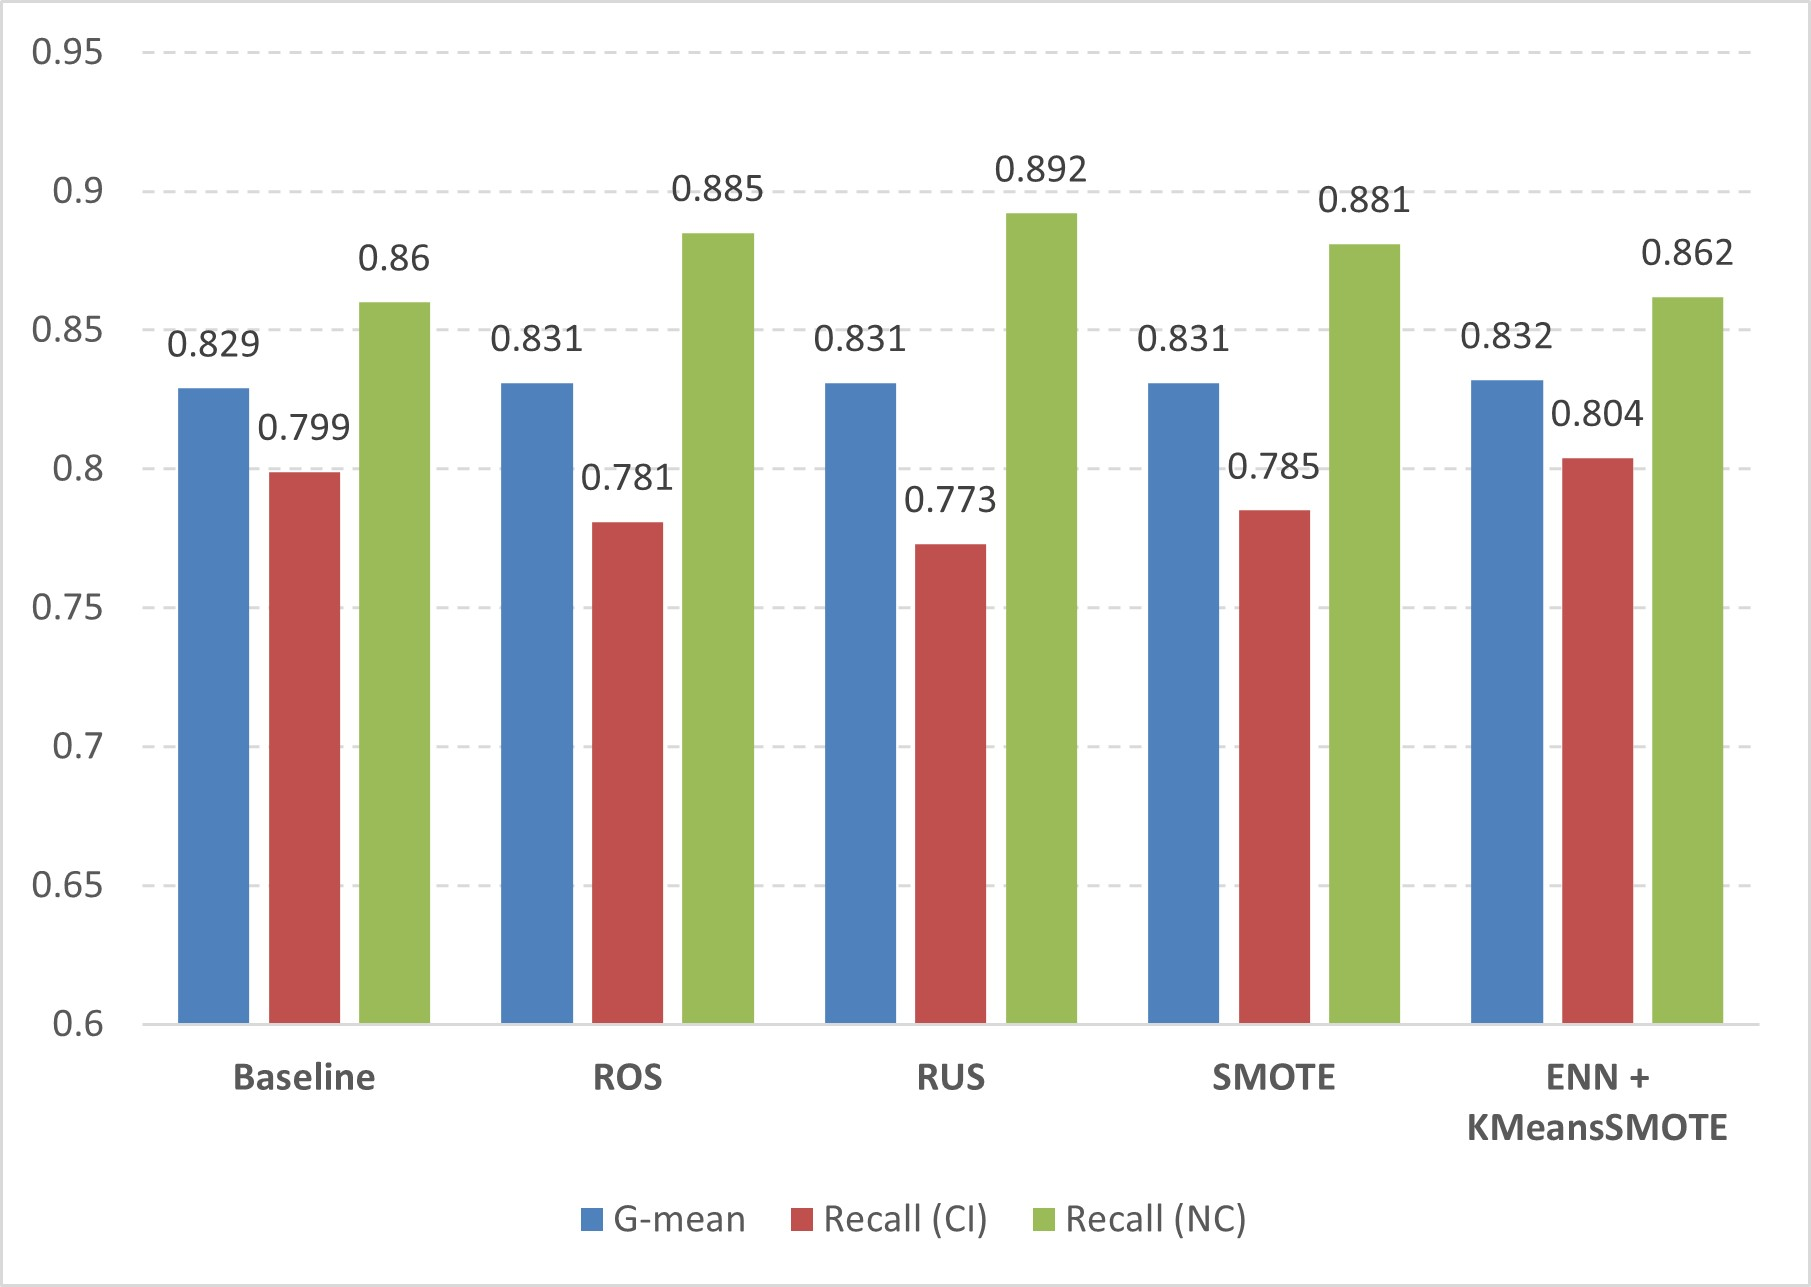
\includegraphics[width=1\textwidth]{figures/data-resampling-task1.jpg}
\caption{Model performance comparison of data resampling methods for the NC vs. CI classification task}
\label{figure:nc_ci_resampling_perf}
\end{figure}

The results show that the baseline model was most affected in its ability to correctly identify the CI class. The baseline RF model achieved a CI recall of only 0.799, although CI is the majority class. The standard resampling methods showed only marginal improvements. Random Oversampling (\acrshort{ROS}) and the Synthetic Minority Over-sampling Technique (\acrshort{SMOTE})  performed similarly. Both methods failed to reduce the high class overlap (N1 of 0.293 and 0.280, respectively) and showed no significant improvement in the CI class recall. Random Undersampling (\acrshort{RUS}) provided a slight reduction in overlap but achieved a G-mean of 0.831 by increasing the recall of the NC class to 0.892 while reducing the recall of the CI class to 0.773.

In contrast, the highest balanced performance (G-mean = 0.832) was achieved using the selected ENN + KMeansSMOTE method. This improvement can be explained by the significant reduction in the class overlap at the instance-level (kDN) to 0.005 and the structural class overlap (N1) to 0.059.  As a result, the recall for the impacted CI class improved to 0.804 while maintaining a high recall for the NC class. \hl{The G-mean improvement of the proposed ENN + KMeansSMOTE method over the baseline was statistically significant (p = 0.026), which confirms that the gain did not occur by random chance.} This confirms the effectiveness of the specialized, overlap-aware strategy.

\subsubsection{Data Resampling Results for the CIND vs. Dementia Classification Task}
\label{sec:resampling_cind_dem}
The baseline characteristics for the CIND vs. dementia task were also analyzed. A low class imbalance was found, with an IR of 1.23. The instance-level class overlap was 0.193 (kDN), and the structural class overlap (N1) was 0.281.

According to the resampling decision algorithm (Algorithm \ref{alg:data-resampling}), data resampling was skipped for this task. This decision was made because the class imbalance was not severe (IR < 2.0) and the instance-level class overlap measures were below the 0.3 threshold. Although a low class imbalance was present, the baseline RF model performance was examined and found to be acceptable in both classes. The baseline model achieved a G-mean of 0.815. It also obtained a recall of 0.807 for the CIND class and 0.824 for the more critical dementia class. This performance was considered a sufficient and balanced starting point for model fine-tuning. Therefore, no resampling methods were applied to this dataset.

In summary, for both classification tasks related to the first research objective, the data complexity was systematically analyzed. The overlap-guided resampling strategy was successfully applied to the NC vs. CI task, creating a more balanced and separable dataset. For the simpler CIND vs. dementia task, the methodology correctly identified that resampling was not necessary. Thus, the original data structure was preserved. This process prepared data for model fine-tuning to achieve the highest possible performance, which is reported in the following subsection.

\subsection{Model Fine-tuning and Selection Results}
After the data resampling step, model fine-tuning and selection were performed. This section shows the results of optimizing and selecting cost-effective models for the two current cognitive status classification tasks. 

\subsubsection{Model Fine-tuning and Selection Results for the NC vs. CI Classification Task} 
The model selection process started by using the cost-effective model selection algorithm (Algorithm \ref{alg:model-selection}) on the grid search hyperparameters fine-tuning results for all five evaluated modeling algorithms. These are k-Nearest Neighbors (\acrshort{KNN}), Logistic Regression (\acrshort{LR}), Light Gradient Boosting Machine (\acrshort{LightGBM}), Random Forest (RF), and Support Vector Machines (\acrshort{SVM}). The goal of the selection algorithm was to find the set of hyperparameter values that produce the most cost-effective model (a model that balances between performance and efficiency). For most classification algorithms (like RF, LR, KNN, and LightGBM), the selection algorithm found a model that was more cost-effective than the best-performing model (the benchmark). This resulted in a considerable efficiency gain, with the highest improvement in training and prediction speed noticed in the LightGBM model. The selection algorithm selected an efficient KNN model with a 1.37 faster prediction speed and the same level of performance as the benchmark model. On the other hand, the algorithm selected the benchmark model for SVM because there was no better alternative. Table~\ref{table:task1_finalists_models} shows a summary of the five finalist fine-tuned models (one model for each algorithm). The table compares their performance and their speed. 

\begin{table}[!ht]
    \centering
    \caption{Summary of fine-tuned models for the NC vs. CI classification task}
    \label{table:task1_finalists_models}
    \newcolumntype{C}{>{\centering\arraybackslash}X}
        \begin{tabularx}{\textwidth}{|C|C|C|C|C|}
        \hline
        \textbf{Model} & 
        \textbf{F1-score (95\% CI)} & 
        \textbf{G-mean (95\% CI)} & 
        \textbf{Training Throughput (Gain)\textsuperscript{1}} & 
        \textbf{Prediction Throughput (Gain)\textsuperscript{1}} \\
        \hline
        KNN & 
        0.844 ($\pm 0.002$) & 
        0.831 ($\pm 0.002$) & 
        $664,626$ $(1.08\times)$ & 
        $12,058$ $(1.37\times)$ \\
        \hline
        LR & 
        0.848 ($\pm 0.002$) & 
        0.842 ($\pm 0.002$) & 
        $1,511,839$ $(1.07\times)$ & 
        $24,641,680$ $(1.09\times)$ \\
        \hline
        LightGBM & 
        0.843 ($\pm 0.002$) & 
        0.837 ($\pm 0.002$) & 
        $227,781$ $(1.28\times)$ & 
        $1,307,402$ $(1.45\times)$ \\
        \hline
        RF & 
        0.849 ($\pm 0.002$) & 
        0.842 ($\pm 0.002$) & 
        $39,407$ $(1.12\times)$ & 
        $263,545$ $(1.21\times)$ \\
        \hline
        SVM & 
        0.848 ($\pm 0.001$) & 
        0.842 ($\pm 0.001$) & 
        $1,721$ & 
        $11,613$ \\
        \hline
        \multicolumn{5}{p{400pt}}{\footnotesize \textsuperscript{1}\hl{Training throughput is reported in training samples per second, and prediction throughput in predictions per second.} Gain is calculated as the ratio of the selected model’s throughput to the benchmark model’s throughput. Values indicate the factor by which training and prediction speed have improved. Gain is not presented when the selected model is the benchmark model.}
    \end{tabularx}
\end{table}

Another assessment was done to choose the best model for this classification task. The five models were assessed based on three main criteria: performance, efficiency (the model's training and prediction speed), and interpretability (how easy it is to explain the model's prediction). From the results in Table~\ref{table:task1_finalists_models}, the LR model was selected as the final model for this classification task.

This choice was made for several reasons. First, LR was one of the models with the highest performance. It achieved an F1-score of 0.848 and a G-mean of 0.842. This performance is very close to the performance of the RF and SVM models. These two models obtained F1-scores of 0.849 and 0.848, respectively. Other models (KNN and LightGBM) had slightly lower performance, so they were not selected. Second, when comparing the top three models (LR, RF, and SVM), their efficiency was the main difference. The LR model was substantially faster than all the other models. The LR model was extremely faster than the SVM model, which had the slowest training and prediction speed among the three best-performing models. Finally, one of the objectives of this study is to develop models that are easy to explain. The coefficients of the LR model can be directly inspected to understand how each feature contributes to the classification. This gives it a clear advantage over the complex and ensemble models like non-linear SVM, RF, and LightGBM models. In the end, the RF and SVM models had a high performance, but they were not the most efficient and interpretable models. LR was the only model that offered the best balance of good performance, great speed, and simple interpretation. Table~\ref{table:lr-fine-tune-task1-apdx} in the appendix presents the hyperparameter fine-tuning results of the LR model.

\subsubsection{Model Fine-tuning and Selection Results for the CIND vs. Dementia Classification Task}
The same process of model fine-tuning and selection was applied to the CIND vs. dementia classification task. The proposed selection algorithm was also used to identify models that optimize the trade-off between accuracy and computational cost. More efficient RF, LightGBM, and KNN models were successfully identified by the selection algorithm. The RF model speed improved by approximately two-times with very minimal decrease in performance. On the other hand, the LR best-performing model was also the most efficient model among the other LR optimized models. Therefore, the best-performing model was retained by the selection algorithm. The performance and throughput of the five fine-tuned models are presented in Table~\ref{table:task2_finalists_models}.

\begin{table}[!ht]
\centering
\caption{Summary of fine-tuned models for the CIND vs. dementia classification task}
\label{table:task2_finalists_models}
\newcolumntype{C}{>{\centering\arraybackslash}X}
    \begin{tabularx}{\textwidth}{|C|C|C|C|C|}
    \hline
    \textbf{Model} &
    \textbf{F1-score (95\% CI)} &
    \textbf{G-mean (95\% CI)} &
    \textbf{Training Throughput (Gain)\textsuperscript{1}} &
    \textbf{Prediction Throughput (Gain)\textsuperscript{1}} \\
        \hline
        KNN &
        0.814 ($\pm 0.004$) &
        0.800 ($\pm 0.003$) &
        $713,015$ $(1.08\times)$ &
        $16,084$ $(2.14\times)$ \\
        \hline
        LR &
        0.842 ($\pm 0.006$) &
        0.828 ($\pm 0.007$) &
        $512,085$ &
        $19,831,465$ \\
        \hline
        LightGBM &
        0.844 ($\pm 0.006$) &
        0.825 ($\pm 0.008$) &
        $146,969$ $(1.24\times)$ &
        $686,674$ $(1.20\times)$ \\
        \hline
        RF &
        0.844 ($\pm 0.005$) &
        0.830 ($\pm 0.006$) &
        $30,959$ $(2.01\times)$ &
        $146,642$ $(2.02\times)$ \\
        \hline
        SVM &
        0.843 ($\pm 0.006$) &
        0.831 ($\pm 0.006$) &
        $531$ $(1.07\times)$ &
        $3,526$ $(1.00\times)$ \\
        \hline
        \multicolumn{5}{p{400pt}}{\footnotesize \textsuperscript{1}\hl{Training throughput is reported in training samples per second, and prediction throughput in predictions per second.} Gain is calculated as the ratio of the selected model’s throughput to the benchmark model’s throughput. Values indicate the factor by which training and prediction speed have improved. Gain is not presented when the selected model is the benchmark model.}
    \end{tabularx}
\end{table}

To determine the optimal model for this specific classification task, a comprehensive assessment was conducted. This is done by evaluating the five optimized models based on performance, efficiency, and interpretability. From these criteria, the LR model was identified as the most suitable cost-effective choice. Regarding performance, a highly competitive group of models was observed. An F1-score of 0.842 was obtained by the LR model. This score is statistically comparable to the RF (0.844), LightGBM (0.844), and SVM (0.843) models. On the other hand, a low F1-score of 0.814 was observed in the KNN model, so it was excluded from the final selection. Because a very similar performance was achieved by the top four models, the final decision was based on computational efficiency. A high speed in training and prediction was demonstrated by the LR model, with a prediction throughput exceeding 19 million samples per second.  This is much faster than LightGBM, RF, and SVM. Furthermore, high interpretability is ensured by the linear nature of the LR model. This is different from the complex structures of ensemble and non-linear models. Consequently, the LR model was selected; although slightly higher accuracy was offered by RF and SVM, they lacked the balance of efficiency and explainability that are needed for this study. The hyperparameter fine-tuning results of the LR model is presented in Table~\ref{table:lr-fine-tune-task2-apdx} in the appendix.

In conclusion, the model fine-tuning and selection process identified the LR model as the suitable cost-effective model for both the NC vs. CI and CIND vs. dementia classification tasks. By selecting a model that is both highly efficient and easy to interpret while maintaining competitive performance, the study successfully addresses the requirements of the first research objective. Finally, the robustness and generalizability of these selected LR models are further assessed in the next section.

\subsection{Model Performance in External Validation}
\label{sec:classification_external_validation}
The generalizability of the selected LR models was assessed for the two current cognitive status classification tasks. This was done by evaluating their performance and clinical utility in the NACC cross-center testing dataset and the independent Alzheimer's Disease Neuroimaging Initiative (\acrshort{ADNI}) dataset. A detailed description of the validation methodology is provided in section \ref{sec:model-validation}.

\subsubsection{External Validation Results for the NC vs. CI Classification Task}
The performance of the LR model in internal and external validations for the NC vs. CI classification task was analyzed. A summary of the performance metrics is presented in Table~\ref{table:nc_ci_results}. Additionally, the Receiver Operating Characteristic (\acrshort{ROC}) curves for the three validation stages are illustrated in Figure~\ref{figure:nc_ci_roc}.

\begin{table}[!ht]
    \centering
    \caption{Performance of the selected logistic regression model in internal and external validation for the NC vs. CI classification task}
    \label{table:nc_ci_results}
    \newcolumntype{C}{>{\centering\arraybackslash}X}
        \begin{tabularx}{\textwidth}{|c|c|C|C|}
            \hline
            \textbf{Metric} & \textbf{Internal CV} & \textbf{NACC Cross-center Validation} & \textbf{ADNI External Validation} \\
            \hline
            AUC & \makecell{0.844 \\ {\small \hl{(0.843--0.846)}}} & \makecell{0.810 \\ {\small \hl{(0.802--0.818)}}} & \makecell{0.825 \\ {\small \hl{(0.807--0.842)}}} \\ \hline
            G-mean & 0.842 & 0.809 & 0.820 \\ \hline
            Sensitivity & 0.785 & 0.777 & 0.739 \\ \hline
            Specificity & 0.903 & 0.843 & 0.911 \\ \hline
            F1-score & 0.848 & 0.823 & 0.833 \\
            \hline
            \multicolumn{4}{p{400pt}}{\footnotesize \hl{AUC: area under the curve, F1-score: harmonic mean of precision and recall, G-mean: geometric mean score, Sensitivity: recall of the CI class, Specificity: recall of the NC class.}}
        \end{tabularx}
\end{table}

\begin{figure}[ht]
    \centering
    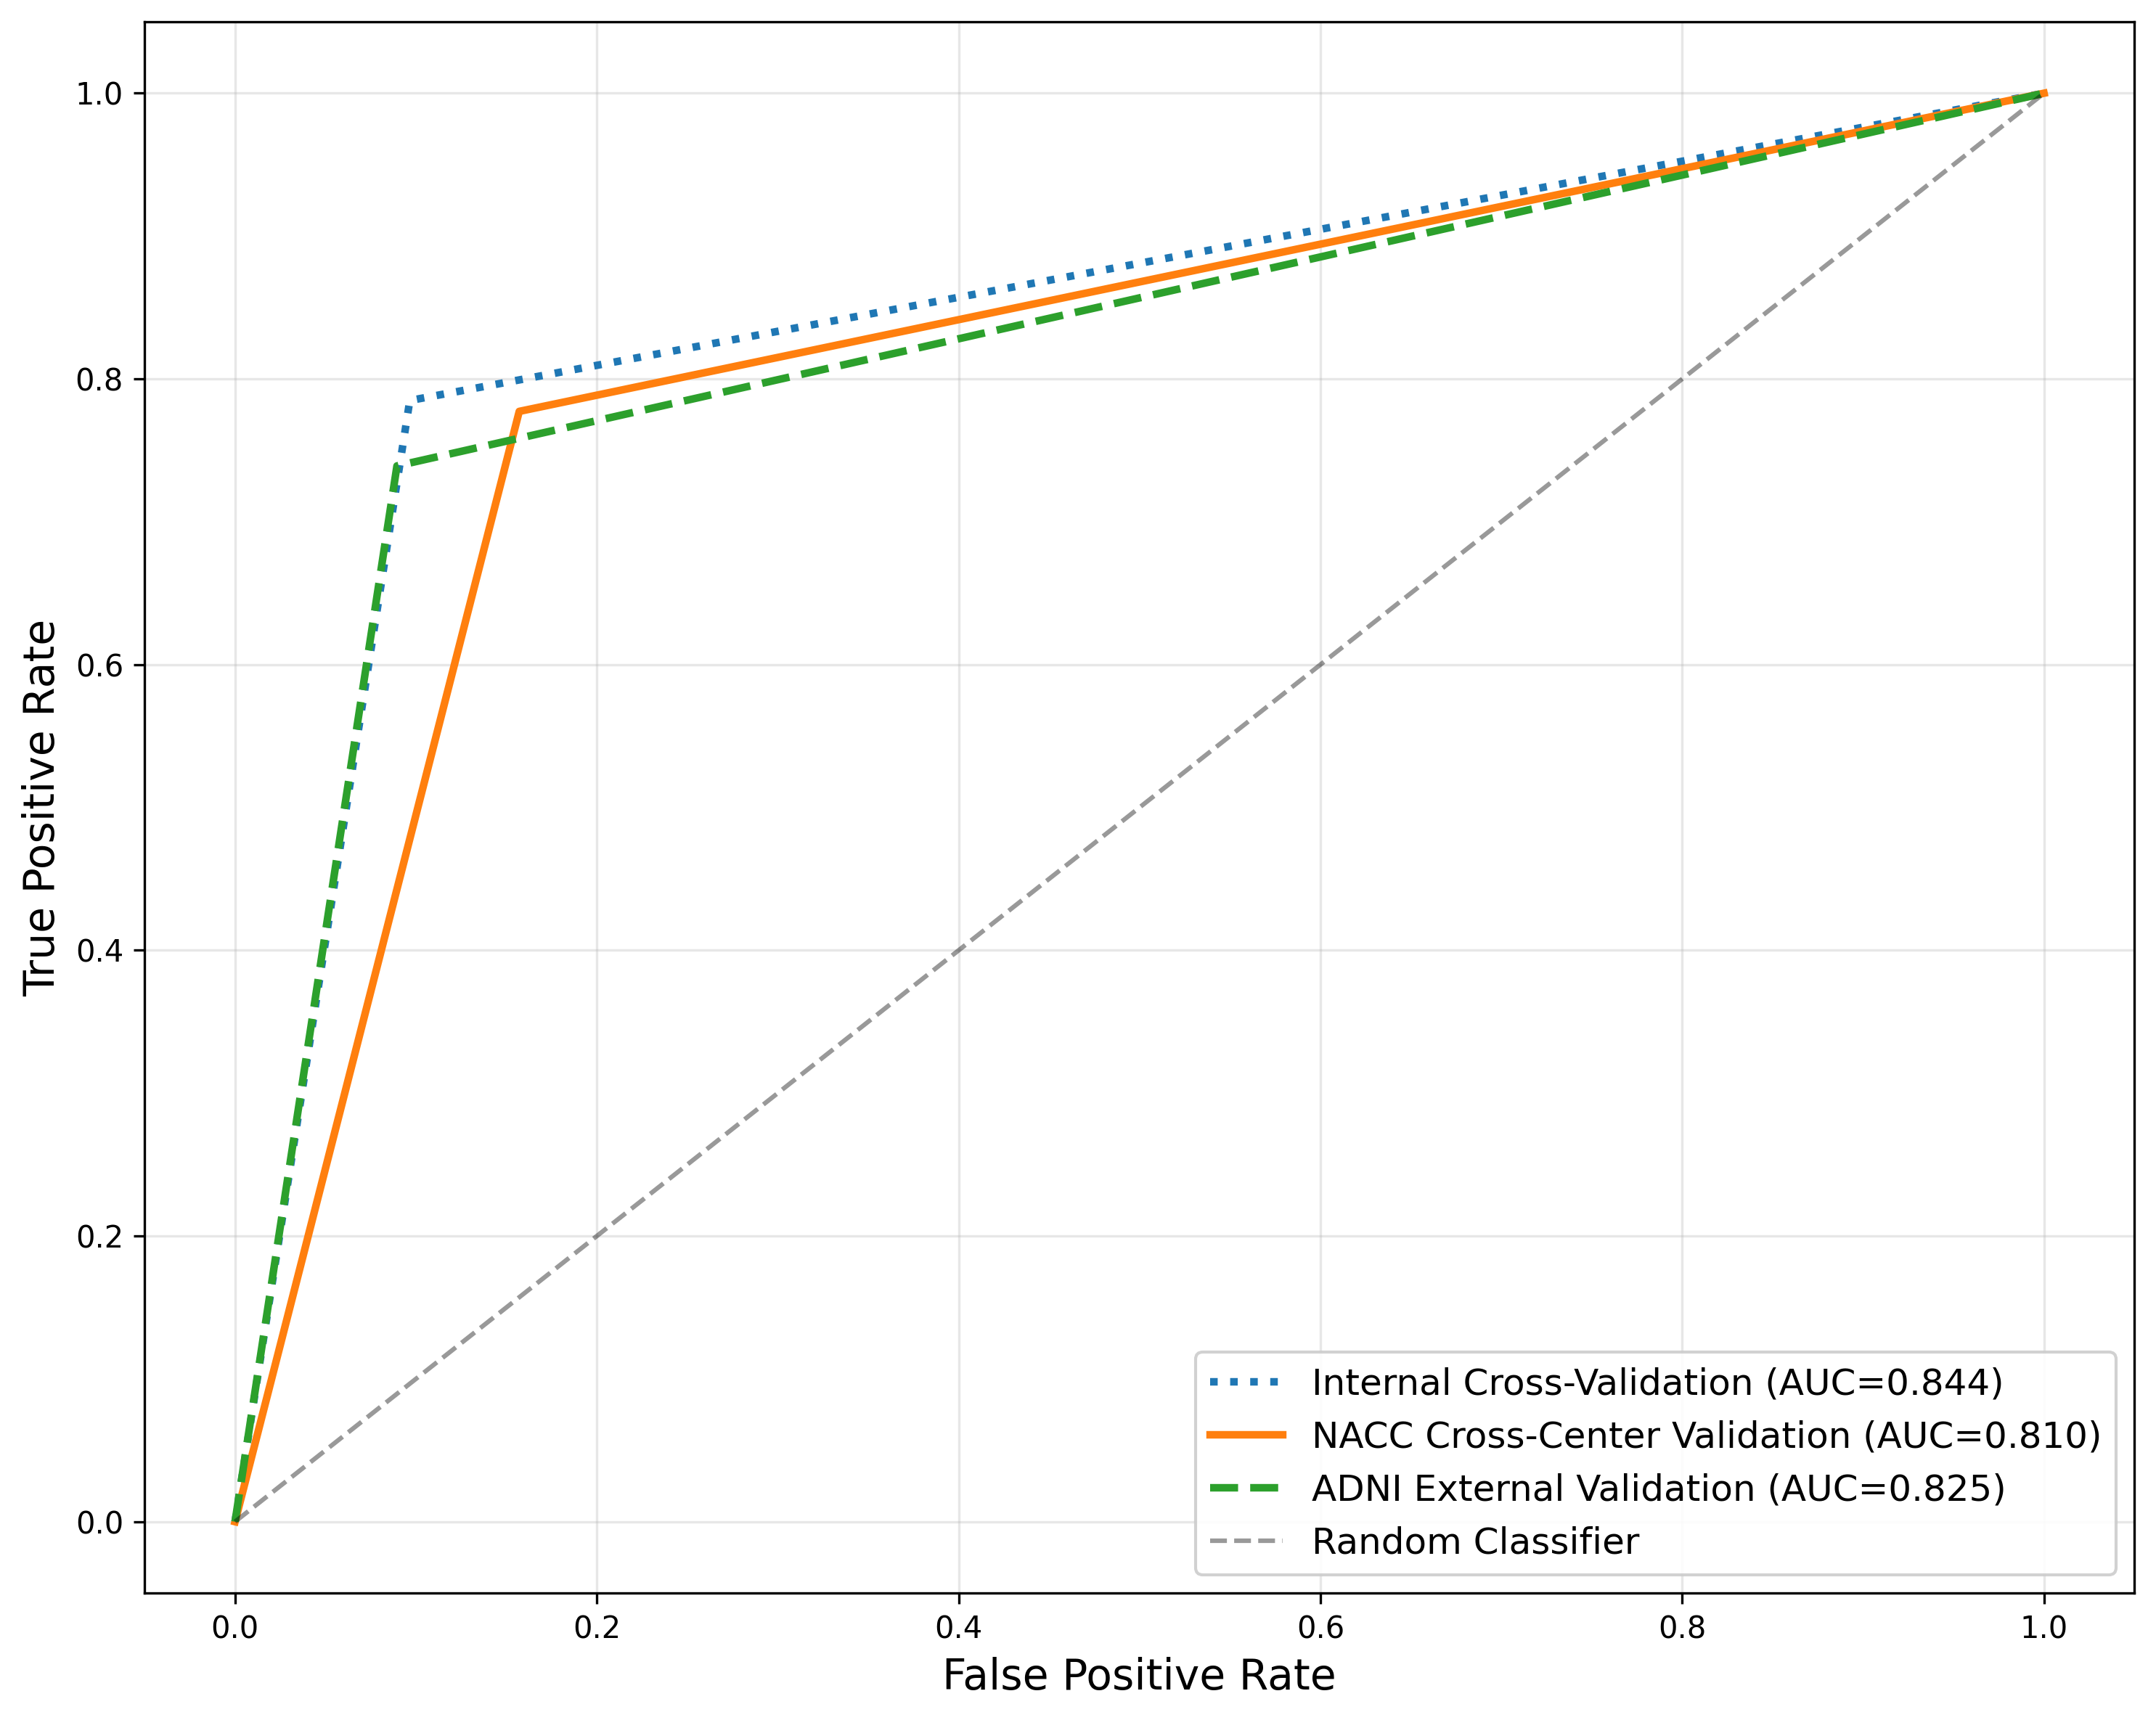
\includegraphics[width=0.7\textwidth]{figures/impaired_classification_all_tests_roc_overlay.png}
    \caption{ROC curves comparing the performance of the logistic regression model for the NC vs. CI classification task}
    \begin{minipage}{\textwidth}
      \footnotesize \hl{The horizontal axis shows the false positive rate (1 -- specificity) and the vertical axis shows the true positive rate (sensitivity). Each curve represents one validation dataset.}
    \end{minipage}
    \label{figure:nc_ci_roc}
\end{figure}

Based on the results of testing the LR model with the NACC cross-center testing dataset, a moderate decrease in overall performance was noticed. A drop of 0.034 in the area under the curve (\acrshort{AUC}) score was recorded, which decreased from 0.844 in the internal cross-validation (CV) to 0.810 in the NACC cross-center validation. A similar decrease was noticed in the G-mean. This performance reduction is due to the major drop in NC recall (specificity) from 0.903 to 0.843, although CI recall (sensitivity) had a minor decrease. The LR struggled to accurately classify NC in the NACC cross-center testing data, compared to the internal CV and the ADNI data. 

Regarding generalizability to the independent ADNI dataset, the LR model achieved high performance, with an AUC score of 0.825. This score is slightly higher than the score of 0.810 in the NACC cross-center validation. The ROC curves in Figure~\ref{figure:nc_ci_roc} demonstrate the performance of the LR in different validations. A notable trade-off between sensitivity and specificity was observed in the ADNI results. Despite a high specificity (0.911), the model's sensitivity score dropped to 0.739, which is a significantly lower score than the score obtained in the NACC cross-center validation. This is likely due to differences in characteristics between the observational NACC study and the ADNI clinical trial. Although high overall accuracy was maintained (as shown by an F1-score of 0.833), the low sensitivity indicates that the LR model is not accurate in classifying CI cases compared to NC cases when used on the ADNI external data. \hl{The reduction in AUC from the internal CV was statistically significant for both the NACC cross-center (p < 0.001) and ADNI (p < 0.001) validations although it should be noted that the very low variance across the five CV folds (SD = 0.002) makes the test highly sensitive to even minor performance differences.} The external validation results are reported with extended performance metrics in Table~\ref{table:lr-complete-perf-task1-apdx} in the appendix.

The prediction of the LR model was calibrated to ensure that it generates probabilities that reflect the actual risk of CI. The results of the model calibration in the two external validation datasets are presented in Figure~\ref{fig:nc_ci_calib_curve}. In the NACC cross-center validation, the uncalibrated LR model tended to overestimate the risk of CI in most probability thresholds (intercept = -0.235). In addition, a slope of 0.191 indicates that the model produced extreme estimations close to 0 and 1. After beta calibration was applied, the model's prediction improved across all probability levels. In general, the Expected Calibration Error (\acrshort{ECE}) decreased significantly from 0.151 to 0.027, and the Brier score improved from 0.168 to 0.136. This indicates that the model's predicted probabilities of CI became closer to the true outcome rates. A different result was observed in the ADNI external validation. In this test, the model underestimated the risk of CI even after applying the beta calibration, which reduced the calibration error from 0.176 to 0.107.

\begin{figure}[ht]
    \centering
    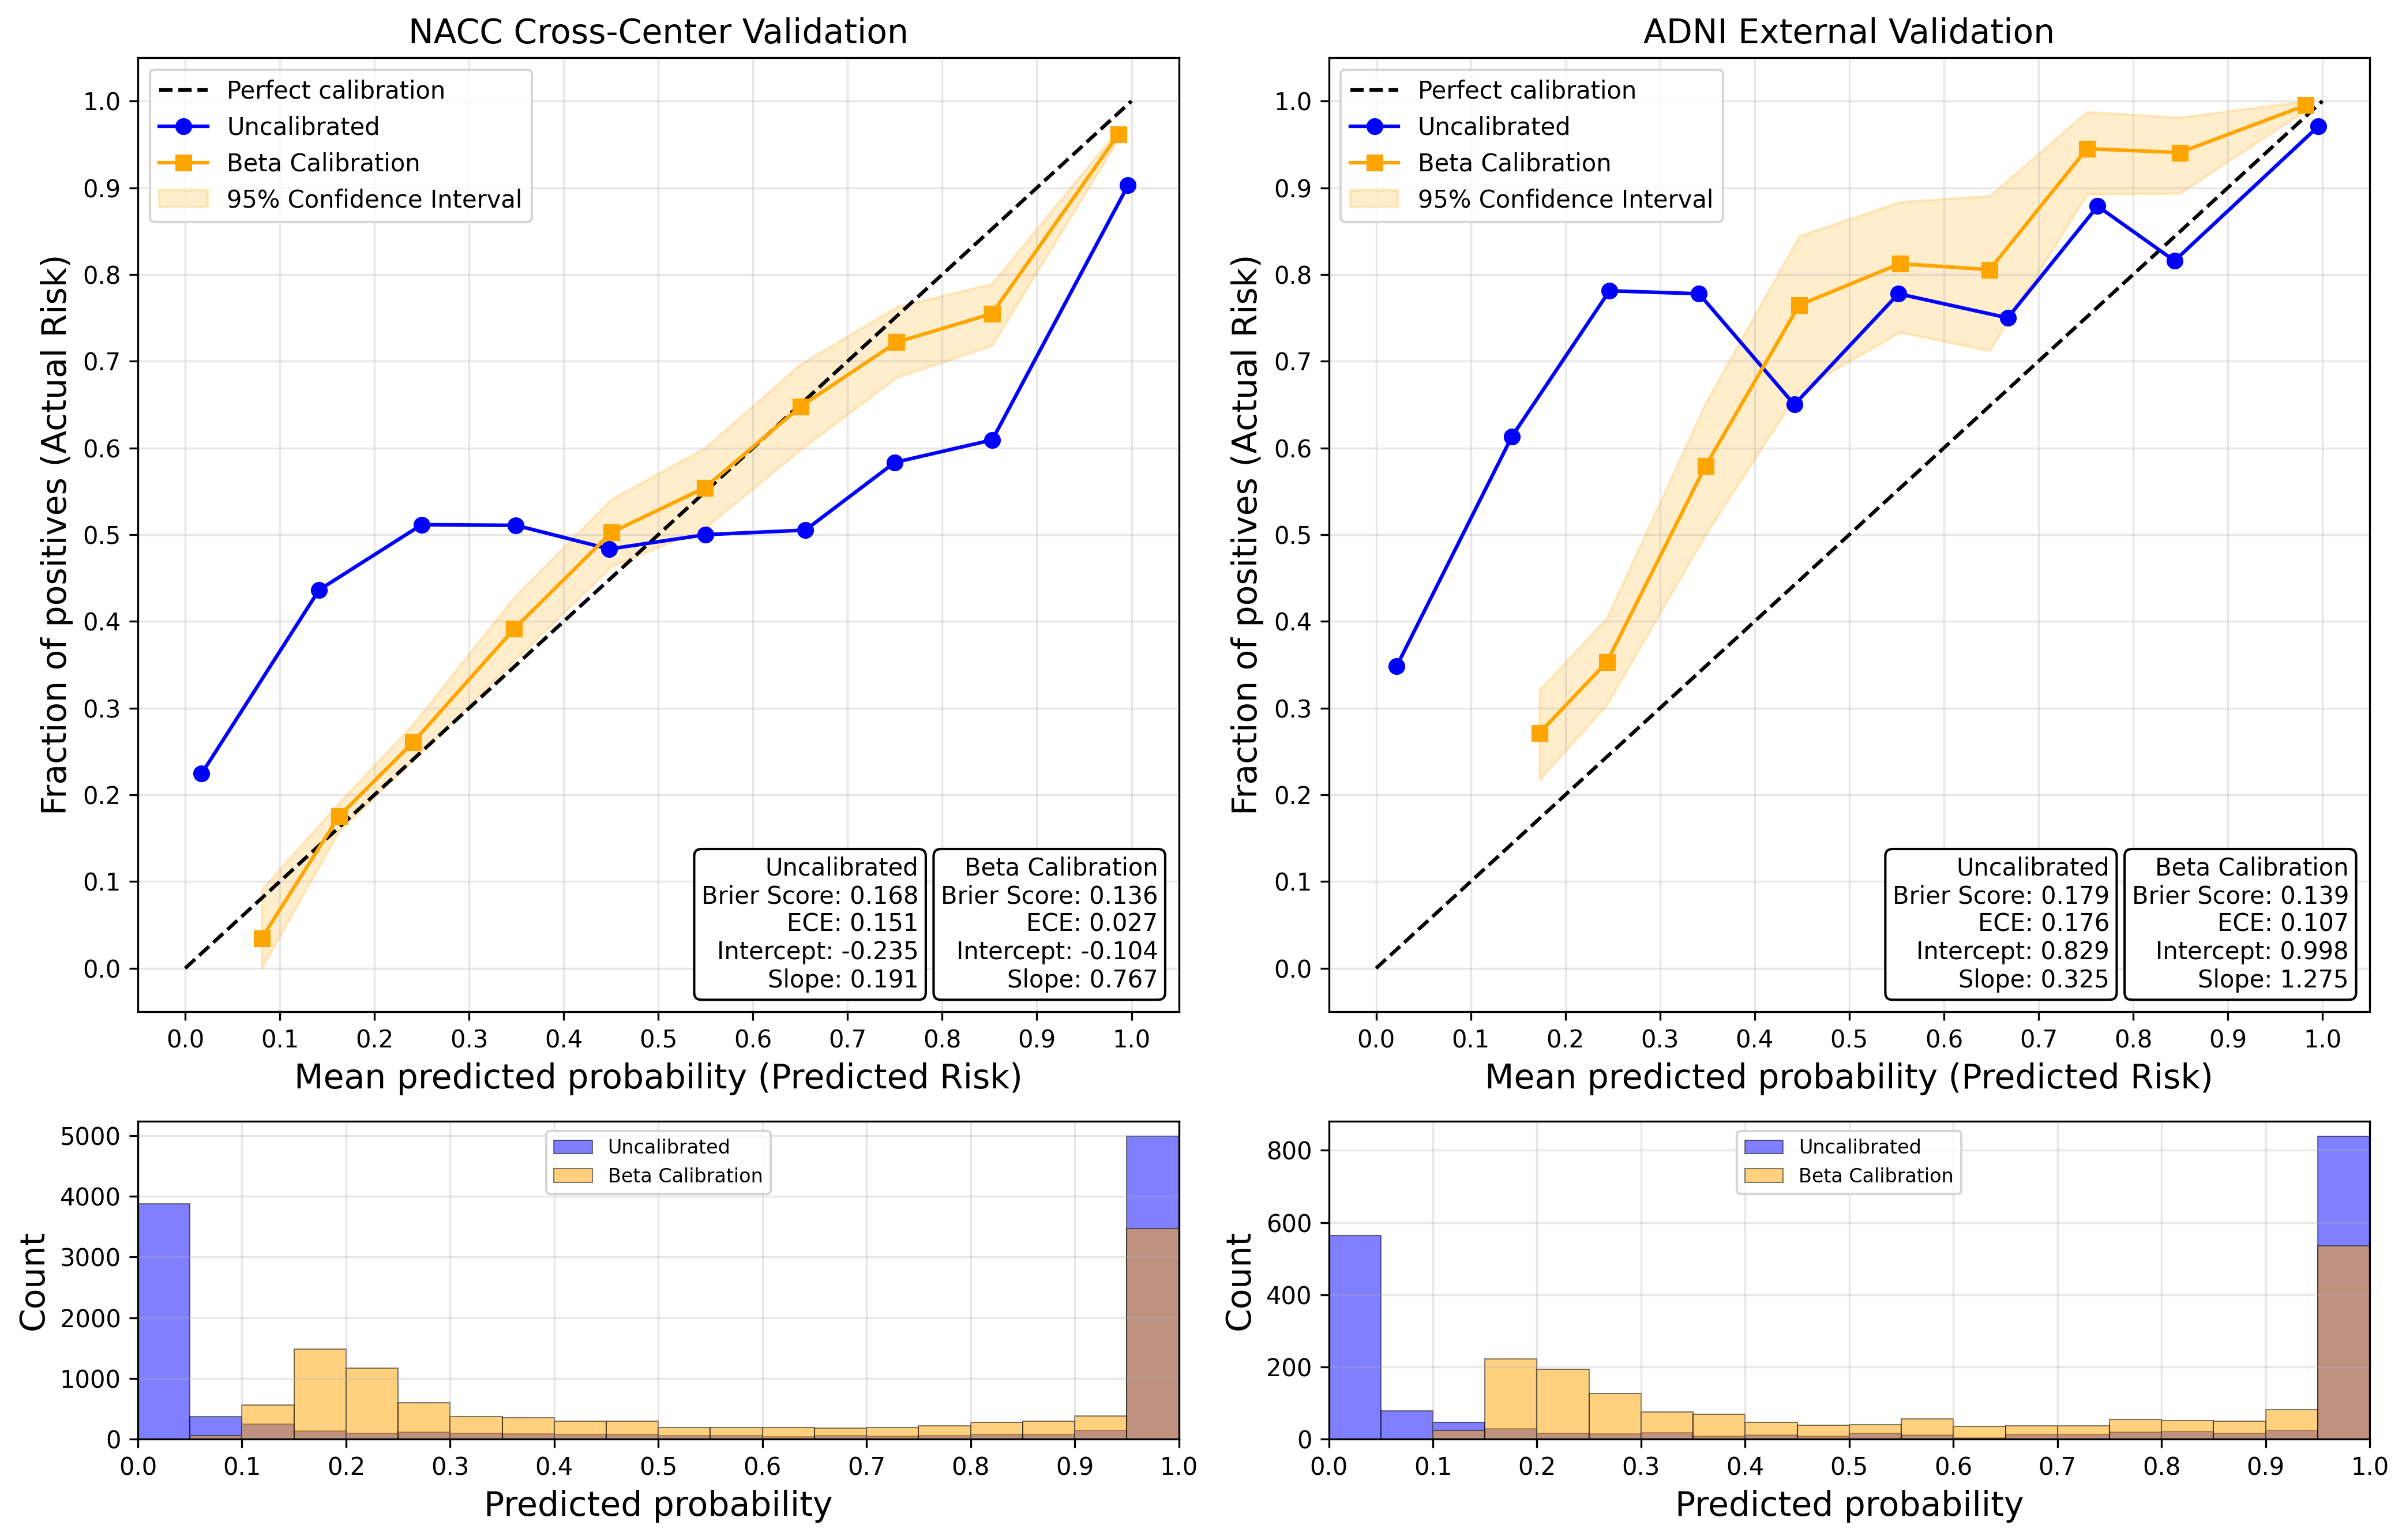
\includegraphics[width=1.0\textwidth]{figures/calibration/impaired_classification_both_calibration_curve.png}
    \caption{Model calibration curves for the NC vs. CI classification task}
    \begin{minipage}{\textwidth}
      \footnotesize \hl{The horizontal axis shows the predicted probability and the vertical axis shows the observed frequency of the positive class. The diagonal line represents perfect calibration, and the curves compare the model before and after beta calibration.}
    \end{minipage}
    \label{fig:nc_ci_calib_curve}
\end{figure}

The calibration of the model prediction supported the clinical utility of the calibrated LR model. According to the Decision Curve Analysis (\acrshort{DCA}) presented in Figure~\ref{fig:nc_ci_dca} the model demonstrated a higher net benefit in probability thresholds ranging from 0.16 to 0.98 in the NACC cross-center validation. This shows that the model has strong clinical utility, outperforming "treat all" and "treat none" strategies for almost any risk cutoff.

\begin{figure}[ht]
    \centering
    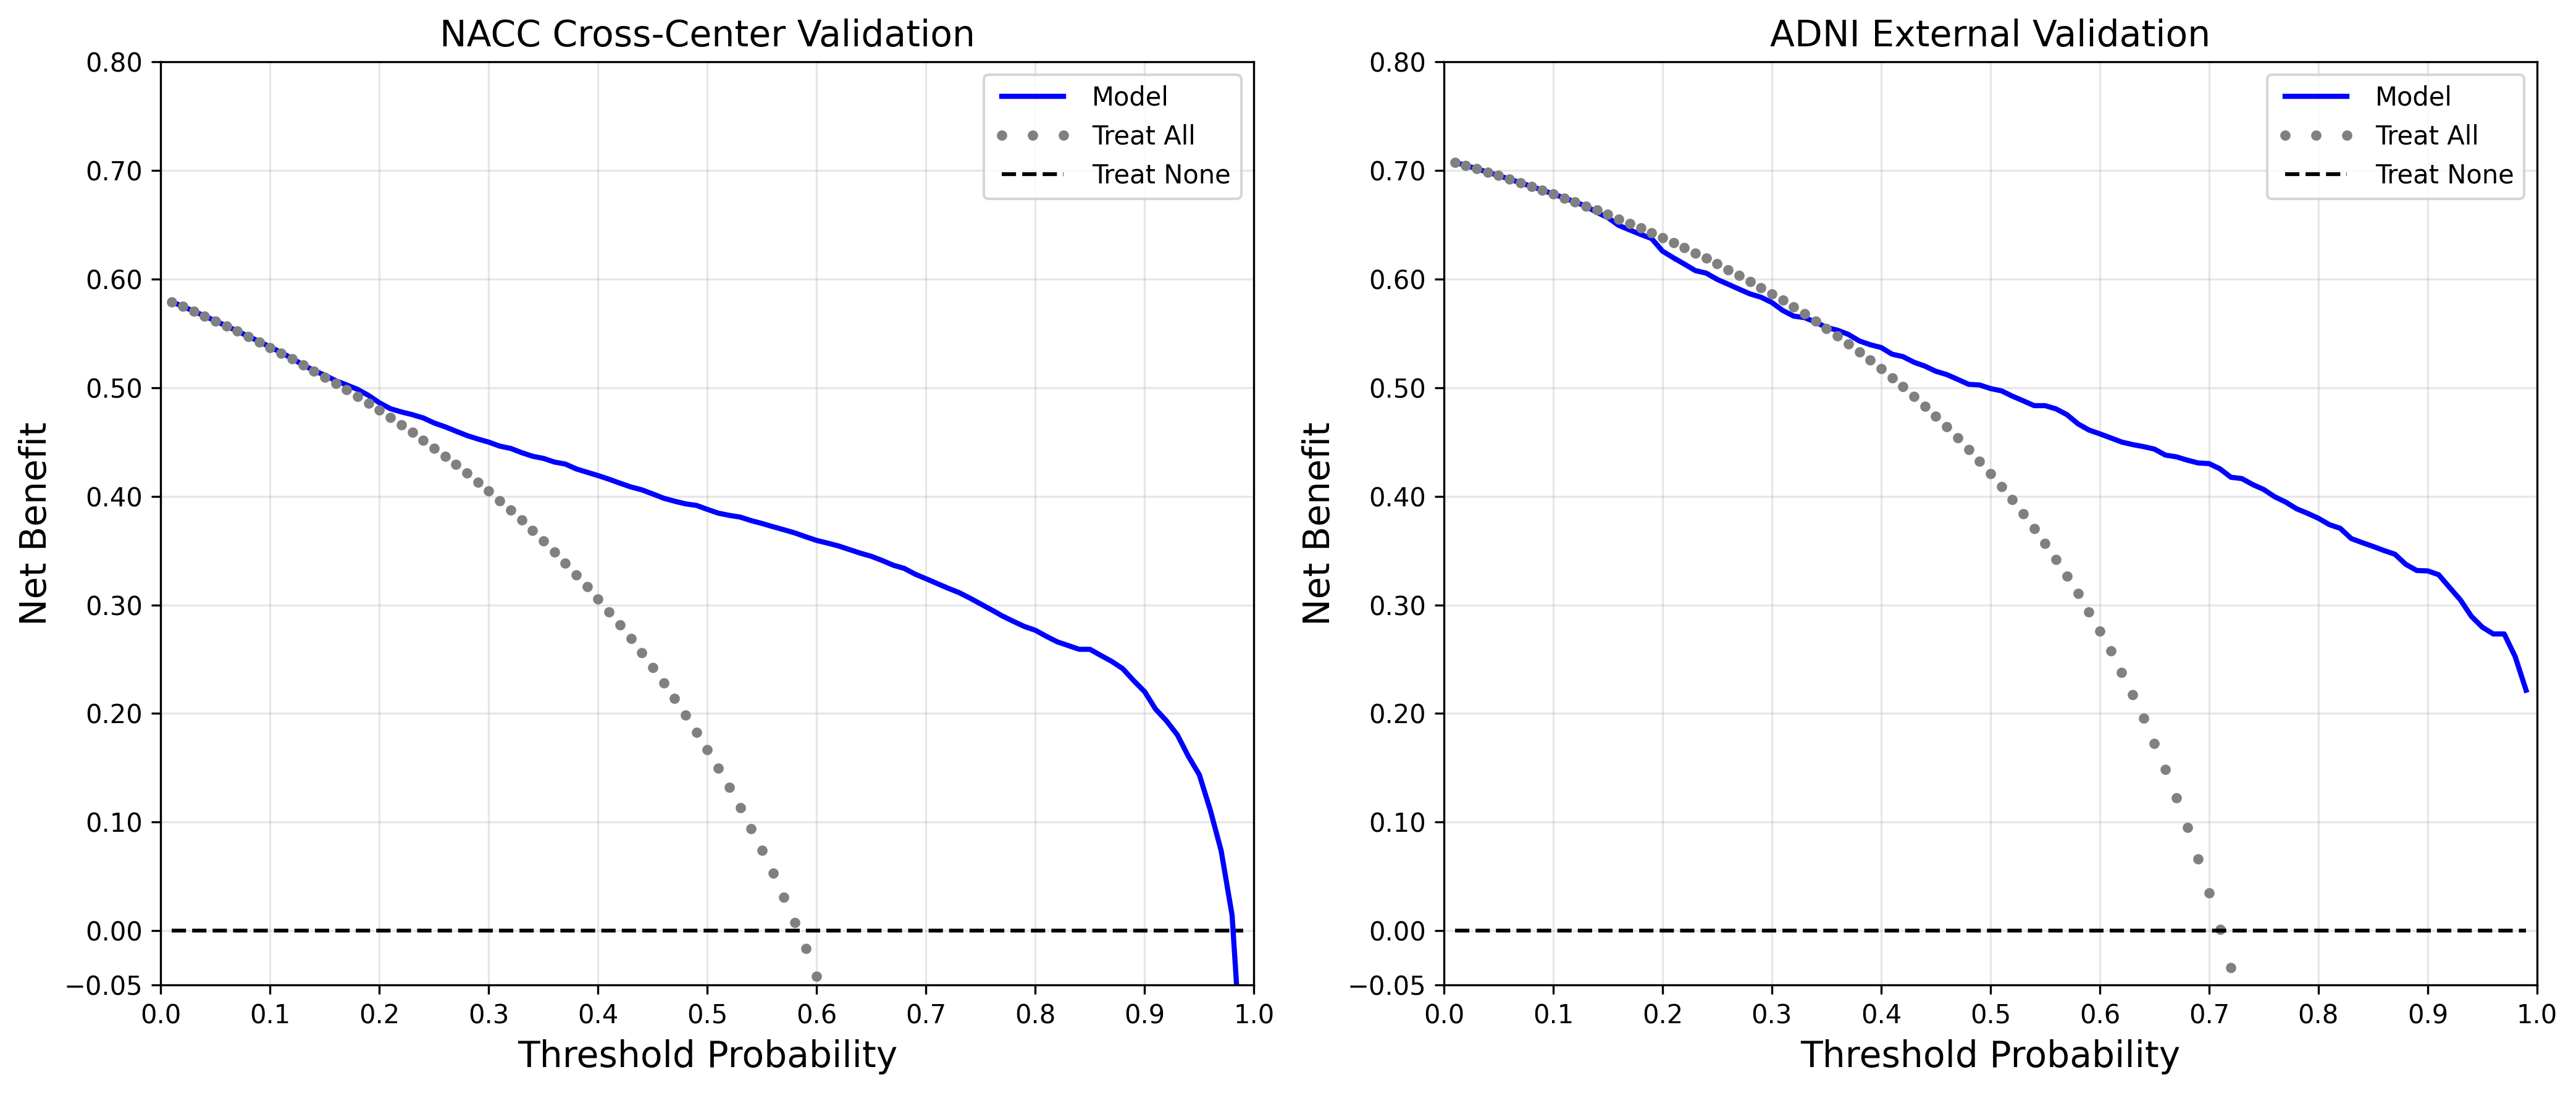
\includegraphics[width=1.0\textwidth]{figures/DCA/impaired_classification_dca_both.png}
    \caption{The decision curve analysis (DCA) for the NC vs. CI classification task}
    \begin{minipage}{\textwidth}
      \footnotesize This figure illustrates the DCA curves of the NACC cross-center validation (left side) and the ADNI external validation (right side). "Treat All" refers to the assumption that all subjects are predicted to have CI, and "Treat None" refers to the assumption that none of the subjects are predicted to have CI.
    \end{minipage}
    \label{fig:nc_ci_dca}
\end{figure}

The clinical utility of the model was limited to thresholds between 0.35 and 0.99 in the ADNI external validation. The model could not identify low-risk subjects and provided no additional benefit compared to the "treat all" strategy at thresholds below 0.35. This could be related to model miscalibration in low probability thresholds observed in the calibration curve in Figure~\ref{fig:nc_ci_calib_curve}.

\subsubsection{External Validation Results for the CIND vs. Dementia Classification Task}
The selected LR model for the CIND vs. dementia classification task was also evaluated to check its performance on unseen data. The results of the internal cross-validation, the NACC cross-center validation, and the ADNI external validation are compared in Table~\ref{table:cind_dementia_results}. The ROC curves for these tests are also presented in Figure~\ref{figure:cind_dementia_roc}.

\begin{table}[!ht]
    \centering
    \caption{Performance of the selected logistic regression model in internal and external validation for the CIND vs. dementia classification task}
    \label{table:cind_dementia_results}
    \newcolumntype{C}{>{\centering\arraybackslash}X}
        \begin{tabularx}{\textwidth}{|c|c|C|C|}
            \hline
            \textbf{Metric} & \textbf{Internal CV} & \textbf{NACC Cross-center Validation} & \textbf{ADNI External Validation} \\
            \hline
            AUC & \makecell{0.828 \\ {\small \hl{(0.821--0.835)}}} & \makecell{0.828 \\ {\small \hl{(0.819--0.837)}}} & \makecell{0.841 \\ {\small \hl{(0.822--0.861)}}} \\ \hline
            G-mean & 0.828 & 0.826 & 0.840 \\ \hline
            Sensitivity & 0.827 & 0.874 & 0.888 \\ \hline
            Specificity & 0.830 & 0.782 & 0.794 \\ \hline
            F1-score & 0.842 & 0.837 & 0.777 \\
            \hline
            \multicolumn{4}{p{400pt}}{\footnotesize \hl{AUC: area under the curve, F1-score: harmonic mean of precision and recall, G-mean: geometric mean score, Sensitivity: recall of the dementia class, Specificity: recall of the CIND class.}}
        \end{tabularx}
\end{table}

\begin{figure}[ht]
    \centering
    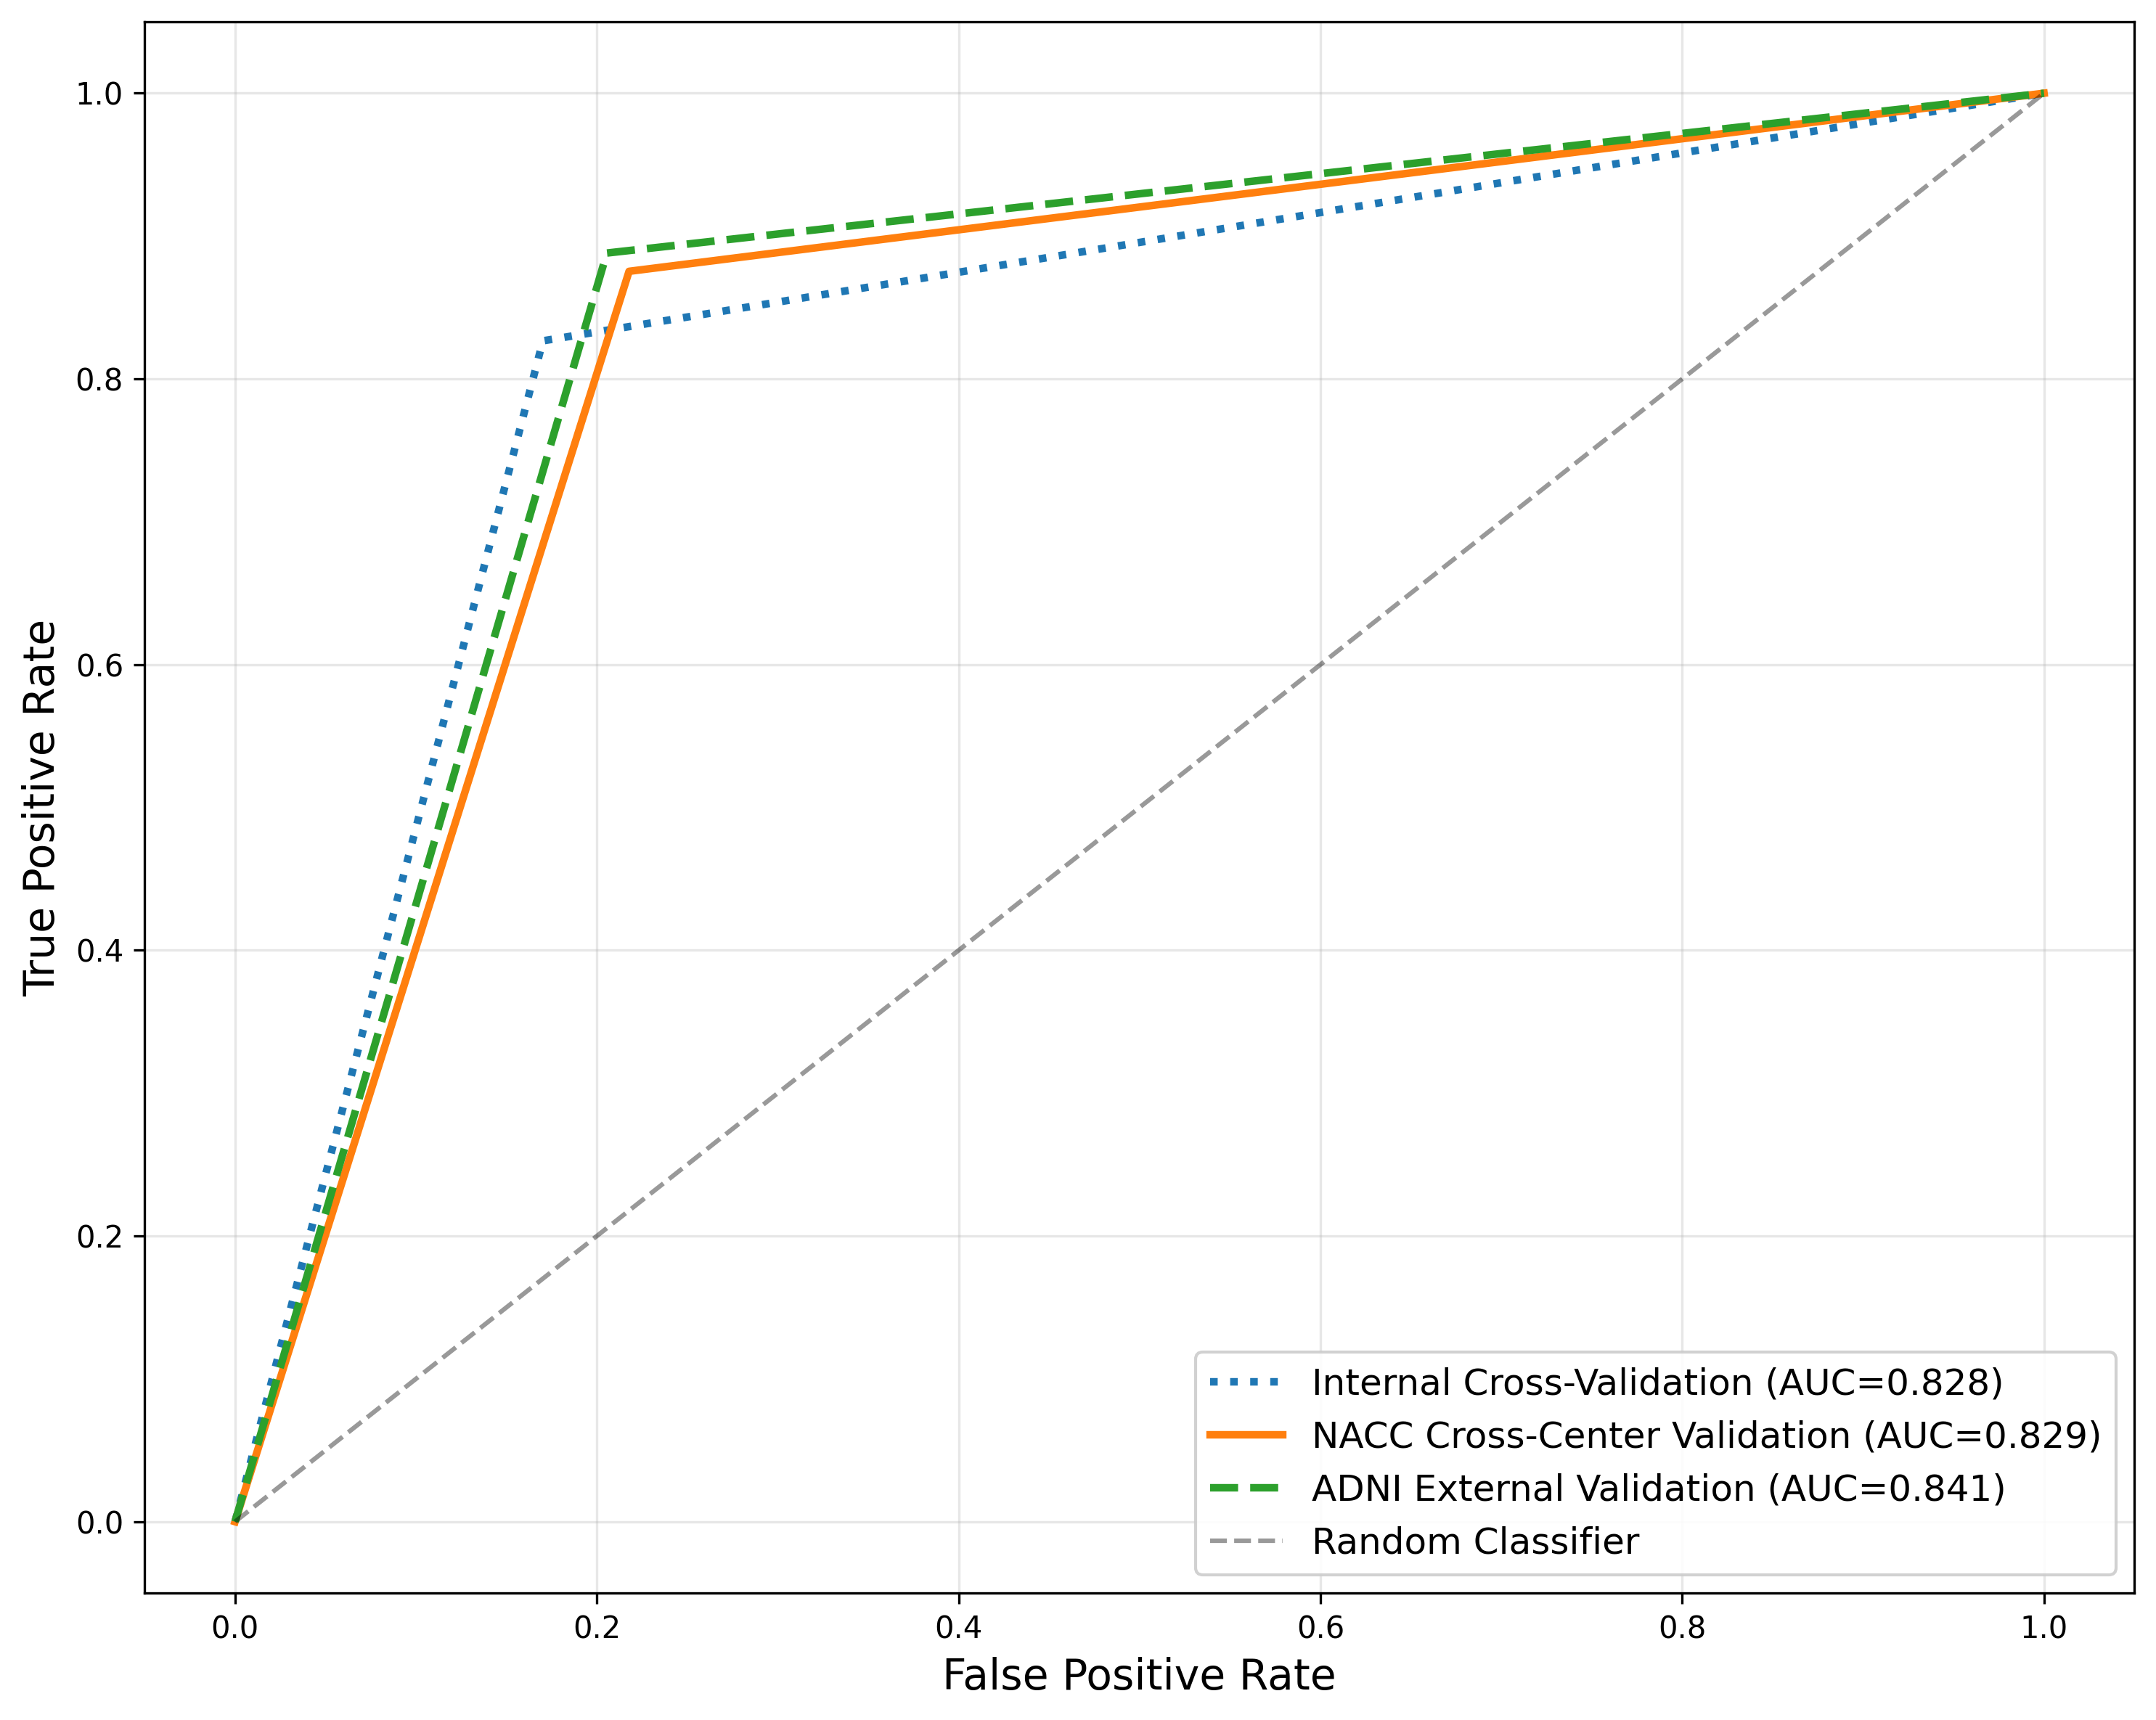
\includegraphics[width=0.7\textwidth]{figures/dementia_classification_all_tests_roc_overlay.png}
    \caption{ROC curves comparing the performance of the logistic regression model for the CIND vs. dementia classification task}
    \begin{minipage}{\textwidth}
      \footnotesize \hl{The horizontal axis shows the false positive rate (1 -- specificity) and the vertical axis shows the true positive rate (sensitivity). Each curve represents one validation dataset.}
    \end{minipage}
    \label{figure:cind_dementia_roc}
\end{figure}

The performance of the LR model on the unseen NACC data was observed to achieve the same AUC as the internal CV and a slight decrease in the G-mean score from 0.828 to 0.826. Additionally, the sensitivity on the NACC cross-center validation increased to 0.874, while the specificity decreased to 0.782. These results indicate that the model correctly classified a high proportion of dementia cases but with a higher false positive rate, which decreased the CIND recall.

The results of the ADNI external validation confirmed that the model is generalizable to different clinical settings. A high AUC of 0.841 was achieved, which exceeded the results of the internal CV and the NACC cross-center validation. This robustness is clearly shown in Figure~\ref{figure:cind_dementia_roc}, where the ADNI curve closely follows or exceeds the other ROC curves. This is a result of a high sensitivity of 0.888, which indicates that the model is highly effective in detecting dementia even in unseen external data. The LR model produced higher precision in classifying both classes (CIND and dementia) in the ADNI external validation compared to the NACC cross-center validation, which can be observed by the G-mean score of 0.840. \hl{The AUC difference between the internal CV and the NACC cross-center validation was not statistically significant (p = 0.912), which supports the close agreement between them, while the higher ADNI AUC was found to be significant (p = 0.038).} Table~\ref{table:lr-complete-perf-task2-apdx} in the appendix provides extended performance metrics of the external validation results.

To ensure that the LR model generates probabilities that accurately reflect the actual risk of dementia, model calibration was performed. The results for both validation datasets are illustrated in Figure~\ref{fig:cind_dementia_calib_curve}. In the NACC cross-center validation, the uncalibrated model already demonstrated strong alignment with the true outcomes. The slope was very close to 1, but the model overestimated the risk of dementia (intercept = -0.461). No improvement was observed after beta calibration because the initial model was already well-calibrated, with an ECE of 0.057 and a Brier score of 0.125.

\begin{figure}[ht]
    \centering
    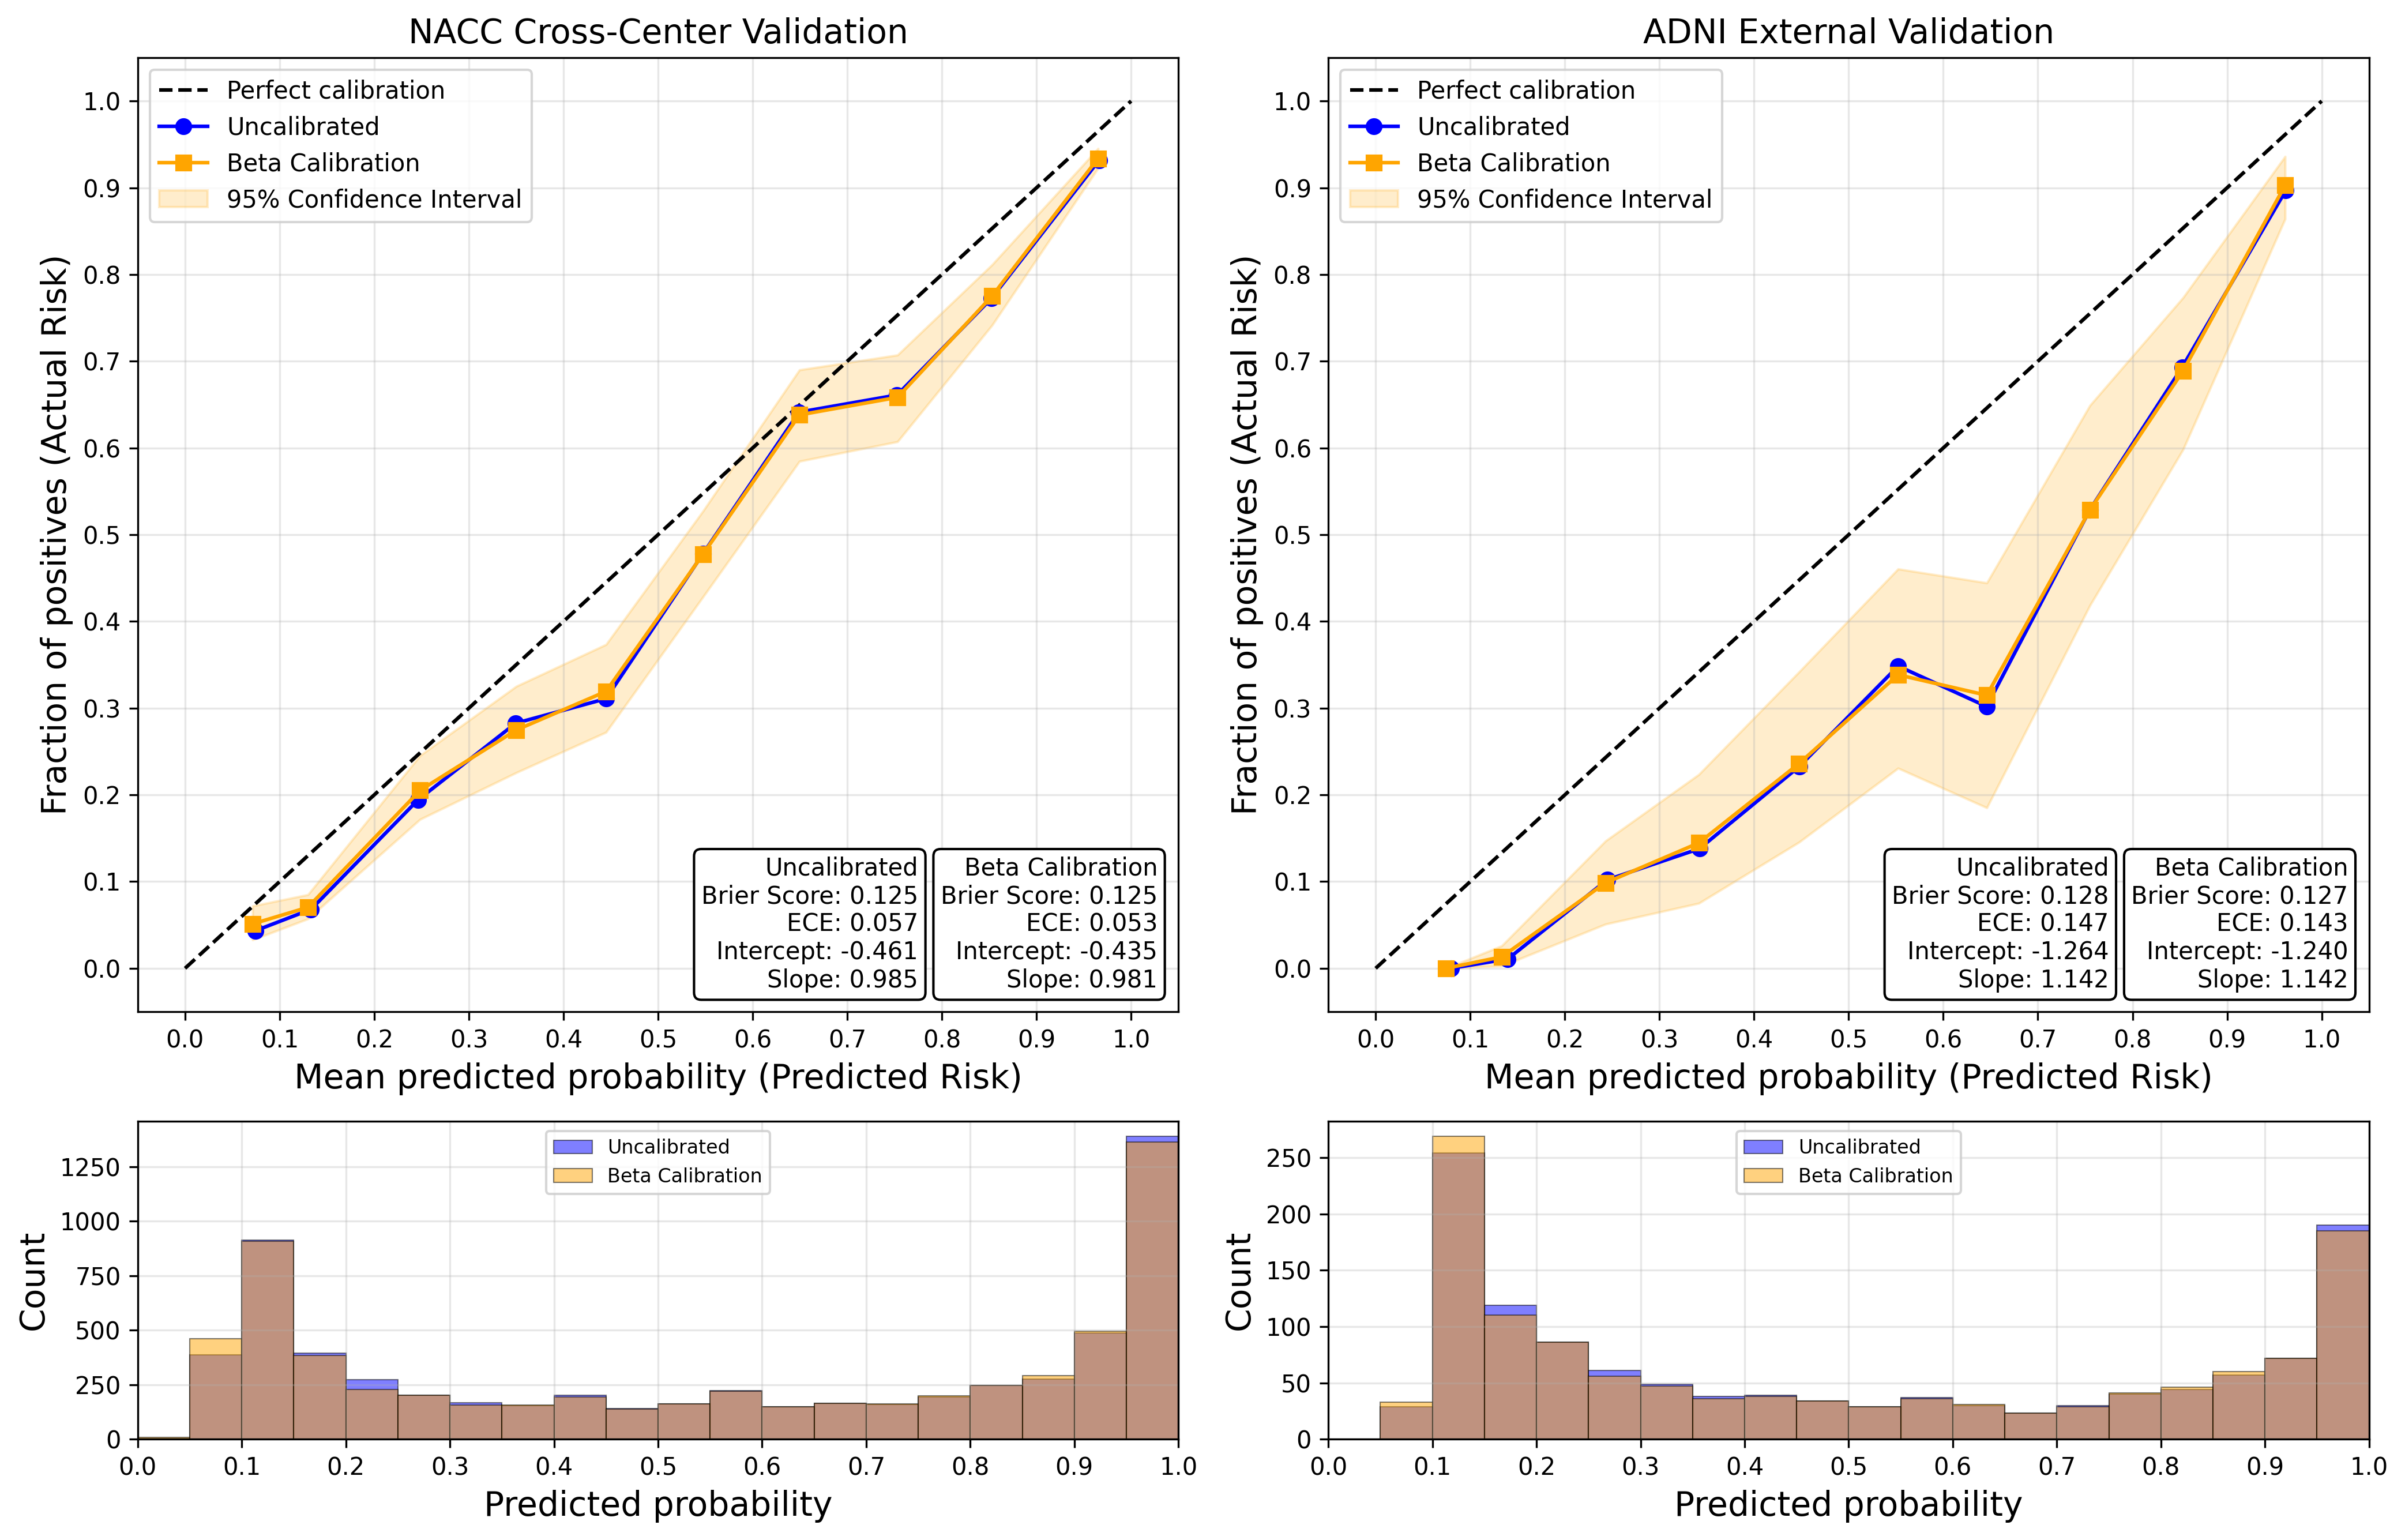
\includegraphics[width=1.0\textwidth]{figures/calibration/dementia_classification_both_calibration_curve.png}
    \caption{Model calibration curves for the CIND vs. dementia classification task}
    \begin{minipage}{\textwidth}
      \footnotesize \hl{The horizontal axis shows the predicted probability and the vertical axis shows the observed frequency of the positive class. The diagonal line represents perfect calibration, and the curves compare the model before and after beta calibration.}
    \end{minipage}
    \label{fig:cind_dementia_calib_curve}
\end{figure}

In contrast, different results were found in the ADNI external validation. A significant overestimation of the risk of dementia was observed, which is indicated by a large negative intercept of -1.264. The miscalibration was not corrected even after beta calibration. This could be explained by the fact that the calibration parameters were learned from the NACC UDS data, which could not correct the specific distribution shifts in the ADNI external dataset. As a result, the beta calibration had almost no improvement, with the ECE remaining high at 0.143.

The clinical utility of the LR model to differentiate CIND from dementia was evaluated using DCA as illustrated in Figure~\ref{fig:cind_dementia_dca}. In the NACC cross-center validation, the model had a higher net benefit than the default strategies ("treat all" and "treat none") in a wide range of probability thresholds (0.11 to 0.99). A similar excellent clinical utility was observed in the ADNI external validation, with a net benefit exceeding default strategies, specifically in probability thresholds between 0.12 and 0.89.

\begin{figure}[ht]
    \centering
    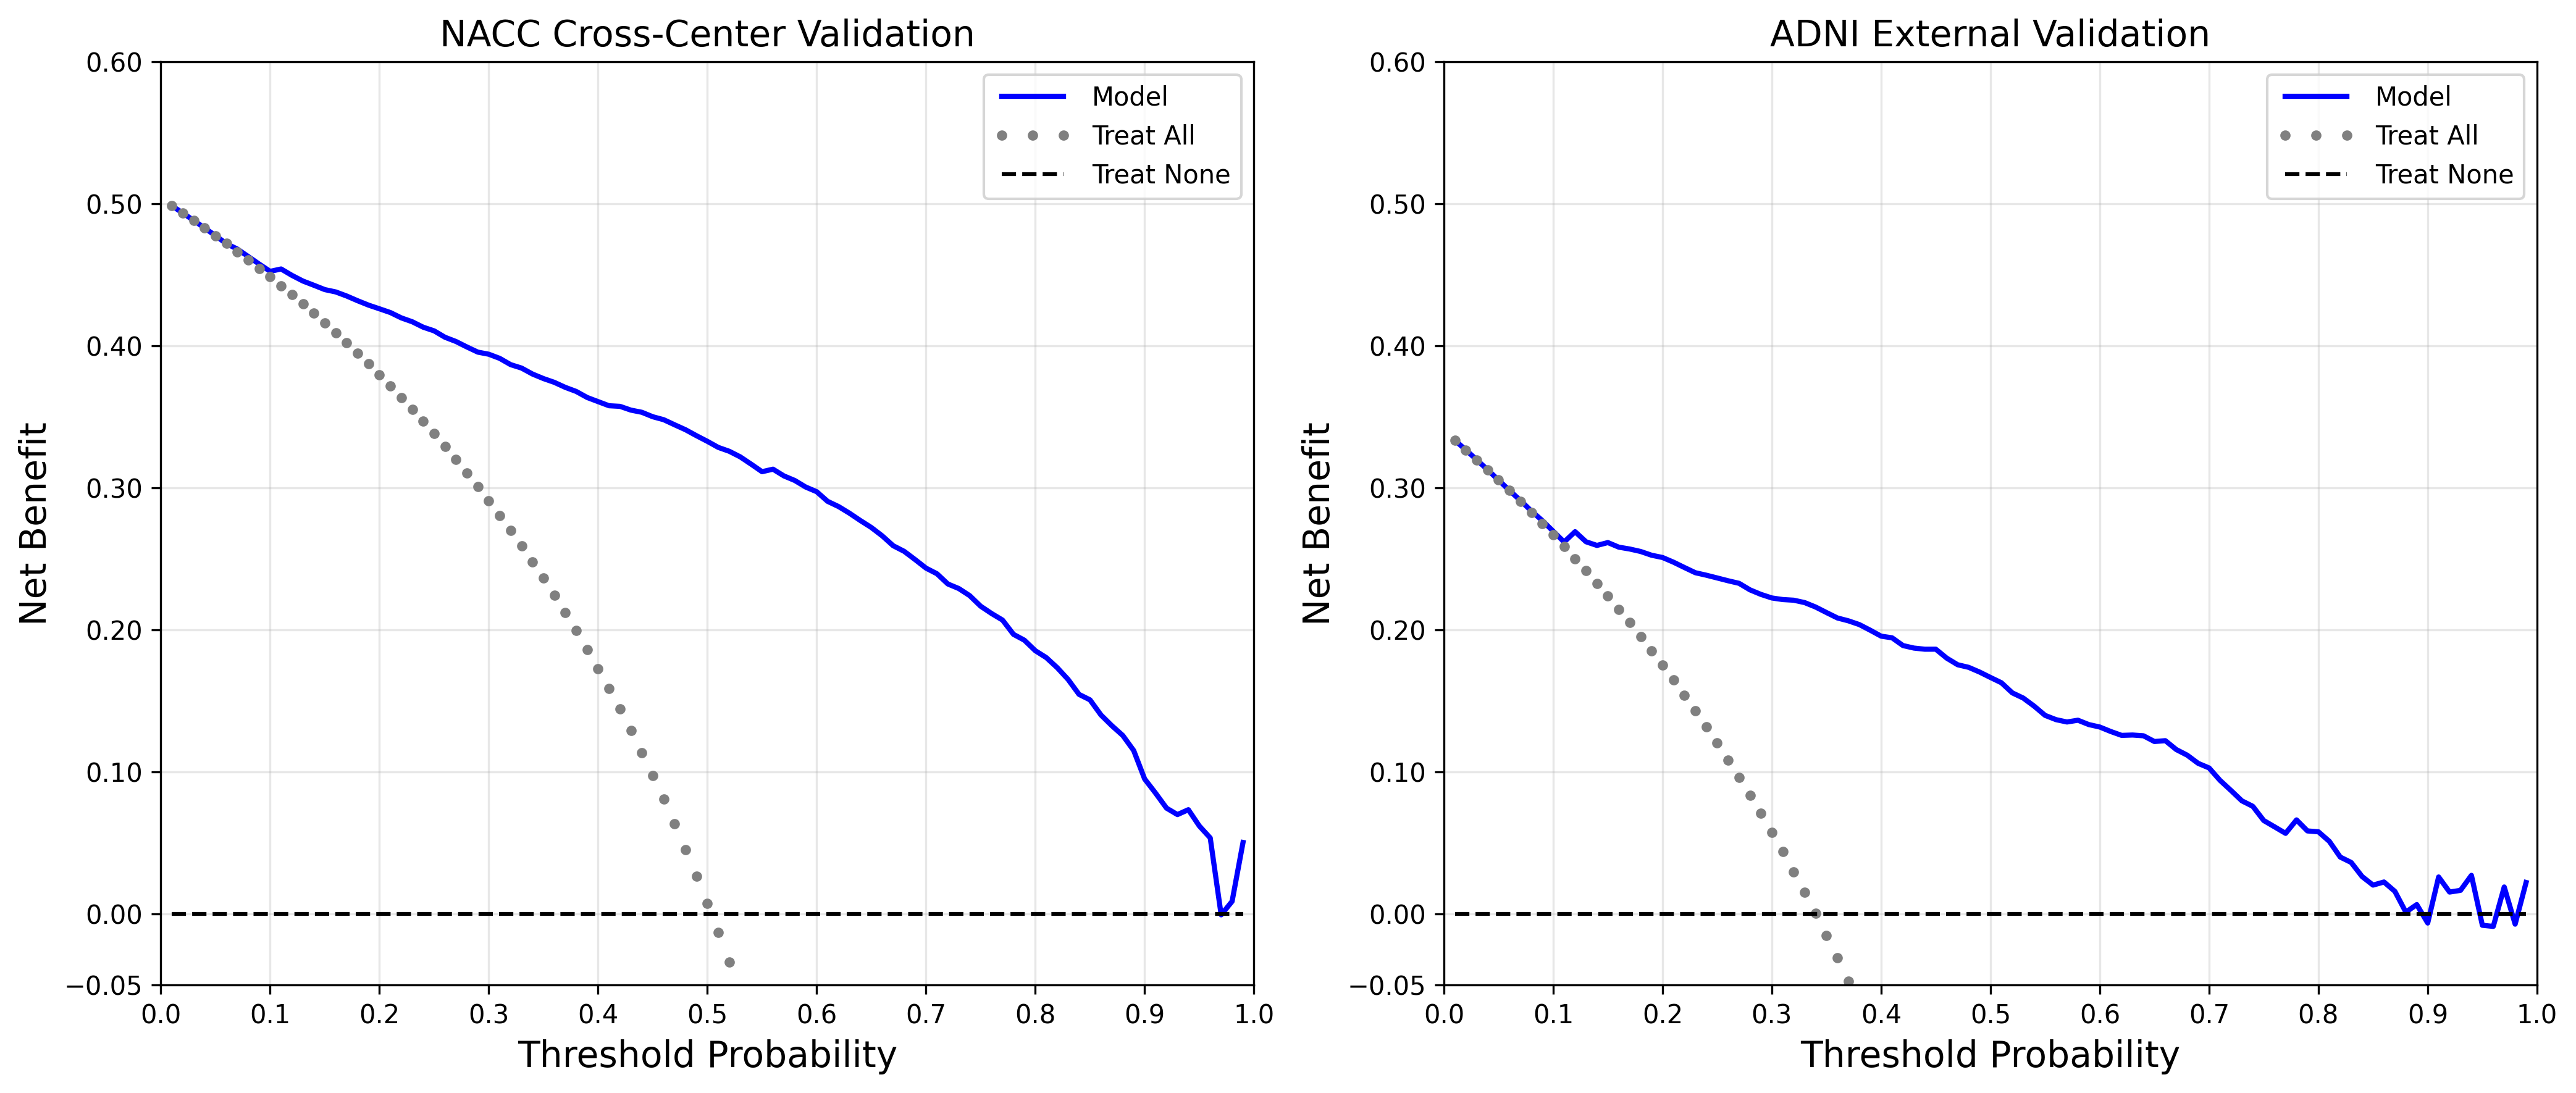
\includegraphics[width=1.0\textwidth]{figures/DCA/dementia_classification_dca_both.png}
    \caption{The decision curve analysis (DCA) for the CIND vs. dementia classification task}
    \begin{minipage}{\textwidth}
      \footnotesize This figure illustrates the DCA curves of the NACC cross-center validation (left side) and the ADNI external validation (right side). "Treat All" refers to the assumption that all subjects are predicted to have dementia, and "Treat None" refers to the assumption that none of the subjects are predicted to have CI.
    \end{minipage}
    \label{fig:cind_dementia_dca}
\end{figure}

Based on the results of the external validation process, it can be concluded that the proposed cost-effective models are reliable and generalizable. The classification models produced a high level of performance, specifically in the detection of critical cases such as dementia, when tested on independent and unseen datasets. Additionally, the models' predictions presented excellent calibration and clinical utility, especially in the NACC cross-center validation. These findings contribute to the achievement of the first research objective of this study. The results demonstrate that a cost-effective machine learning model trained on accessible data can accurately classify the current cognitive status across different clinical settings.

\subsection{Model Explainability Results}
\label{sec:cls-xai}

\subsubsection{Model Explainability Results for the NC vs. CI Classification Task}
The global feature importance ranking of this task is provided in Figure~\ref{figure:nc_ci_feature_importance} for both external validation datasets. The features are sorted on the basis of their mean absolute SHapley values obtained from the SHapley Additive exPlanations (\acrshort{SHAP}). The feature importance ranking in both external validation datasets is highly consistent, with Spearman’s coefficient of 0.93 ($p$ < 0.05). This strong positive correlation indicates that the model relies on a stable set of clinical patterns to predict cognitive impairment, regardless of the population or data source. In both tests, functional activities were identified as the most critical predictors. Specifically, REMDATES, TRAVEL, BILLS and TAXES were consistently ranked as the top four most important features. This indicates the influence of executive function on the model's classification of cases as NC or CI. On the other hand, demographic factors such as NACCAGE (age) and SEX showed less importance compared to the other features. MEMPROB ranked higher in the NACC cross-center validation compared to the ADNI external validation. This might reflect the diagnostic procedures used in these different studies. In addition, the feature importance rank slightly differed in the least important features. NACCAGE ranked as the least important feature after ANX and SEX in the ADNI external validation compared to the NACC cross-center validation.

\begin{figure}[ht]
    \centering
    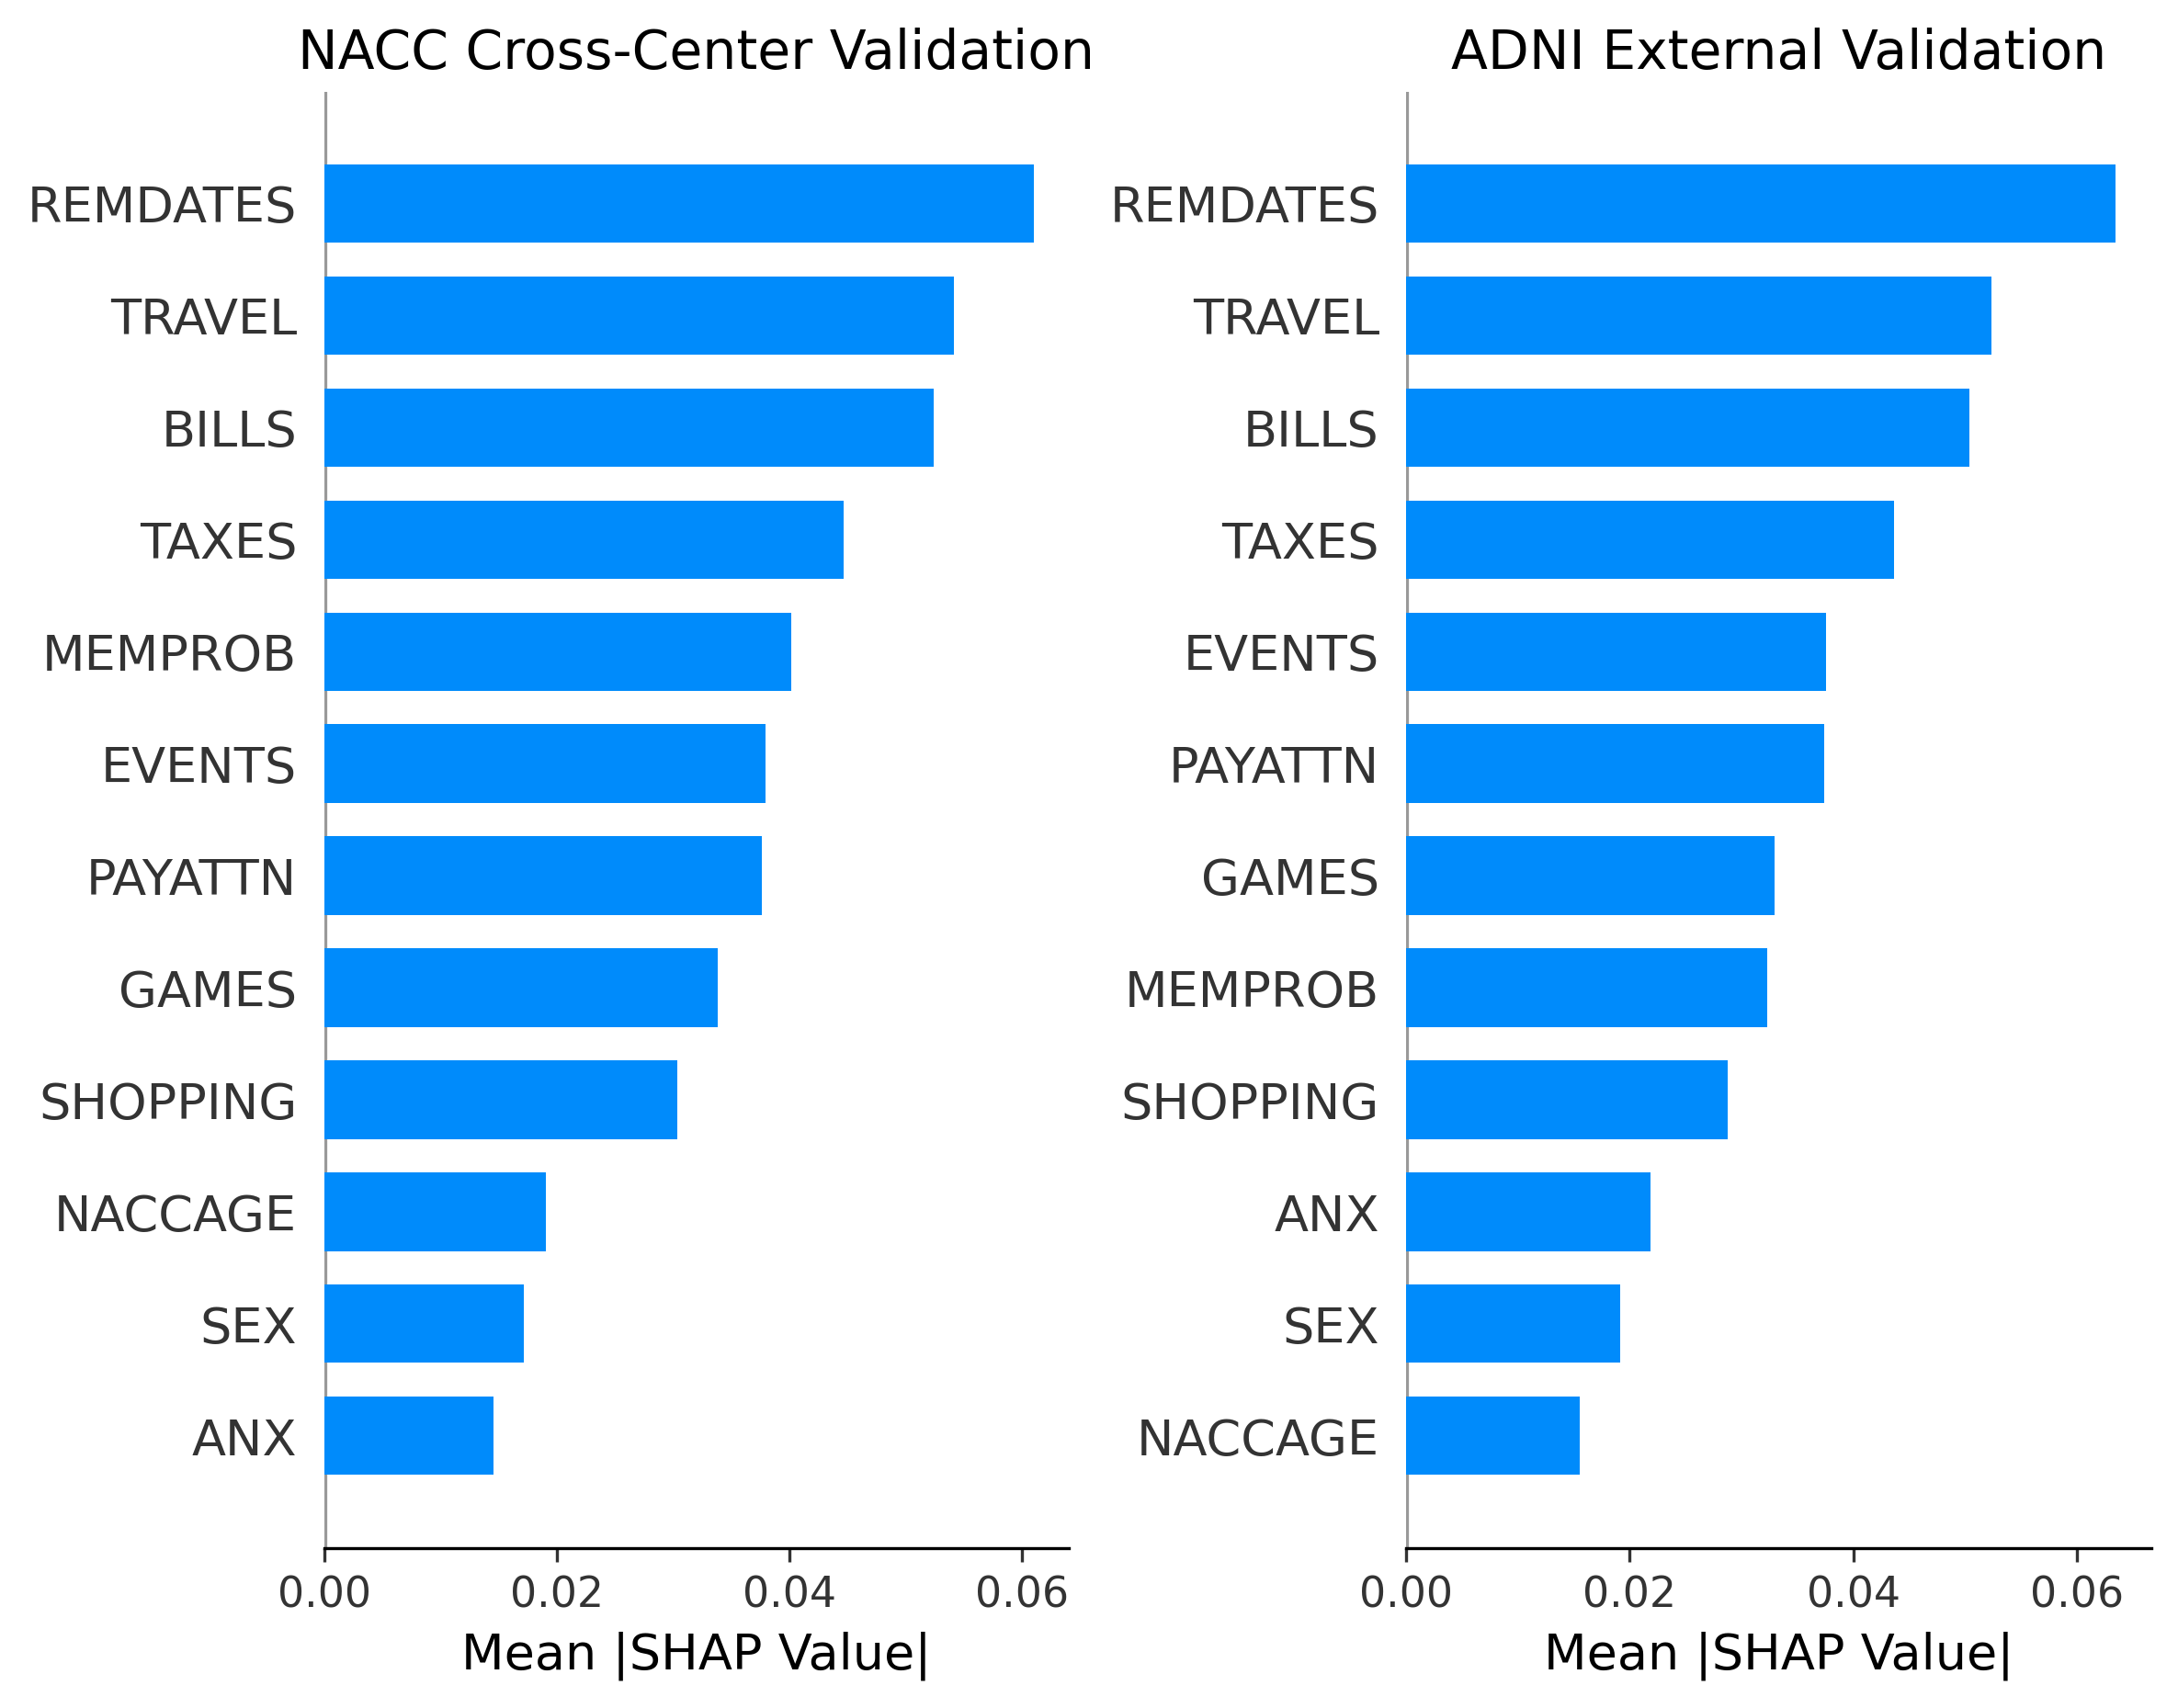
\includegraphics[width=1.0\textwidth]{figures/XAI/impaired_classification_both_feature_importance_comparison.png}
    \caption{Feature importance in the NACC cross-center validation and the ADNI external validation for the NC vs. CI classification task}
    \begin{minipage}{\textwidth}
      \footnotesize \hl{The bars represent the mean absolute SHAP value of each feature, which ranks the contribution of the feature to the model prediction in the two validation datasets.}
    \end{minipage}
    \label{figure:nc_ci_feature_importance}
\end{figure}

Regarding the local explanation, the waterfall plots in Figure~\ref{figure:nc_ci_pos_waterfall} explain the prediction of two correctly classified CI instances from the ADNI external validation. Both instances have similar predicted probabilities of approximately 55\%. \textit{Instance A} predicted with CI due to reported memory problems (MEMPROB) and anxiety (ANX) despite the ability to normally perform all functional activities based on the items in the FAQ. On the other hand, \textit{Instance B} represents an older subject who suffers from difficulty in handling financial matters, specifically paying bills (BILLS) and doing taxes (TAXES). This comparison highlights the model's capability to detect CI through different pathways: one driven by memory and psychological symptoms (\textit{Instance A}) and another driven by specific functional decline in complex tasks (Instance B).

\begin{figure}[ht]
    \centering
    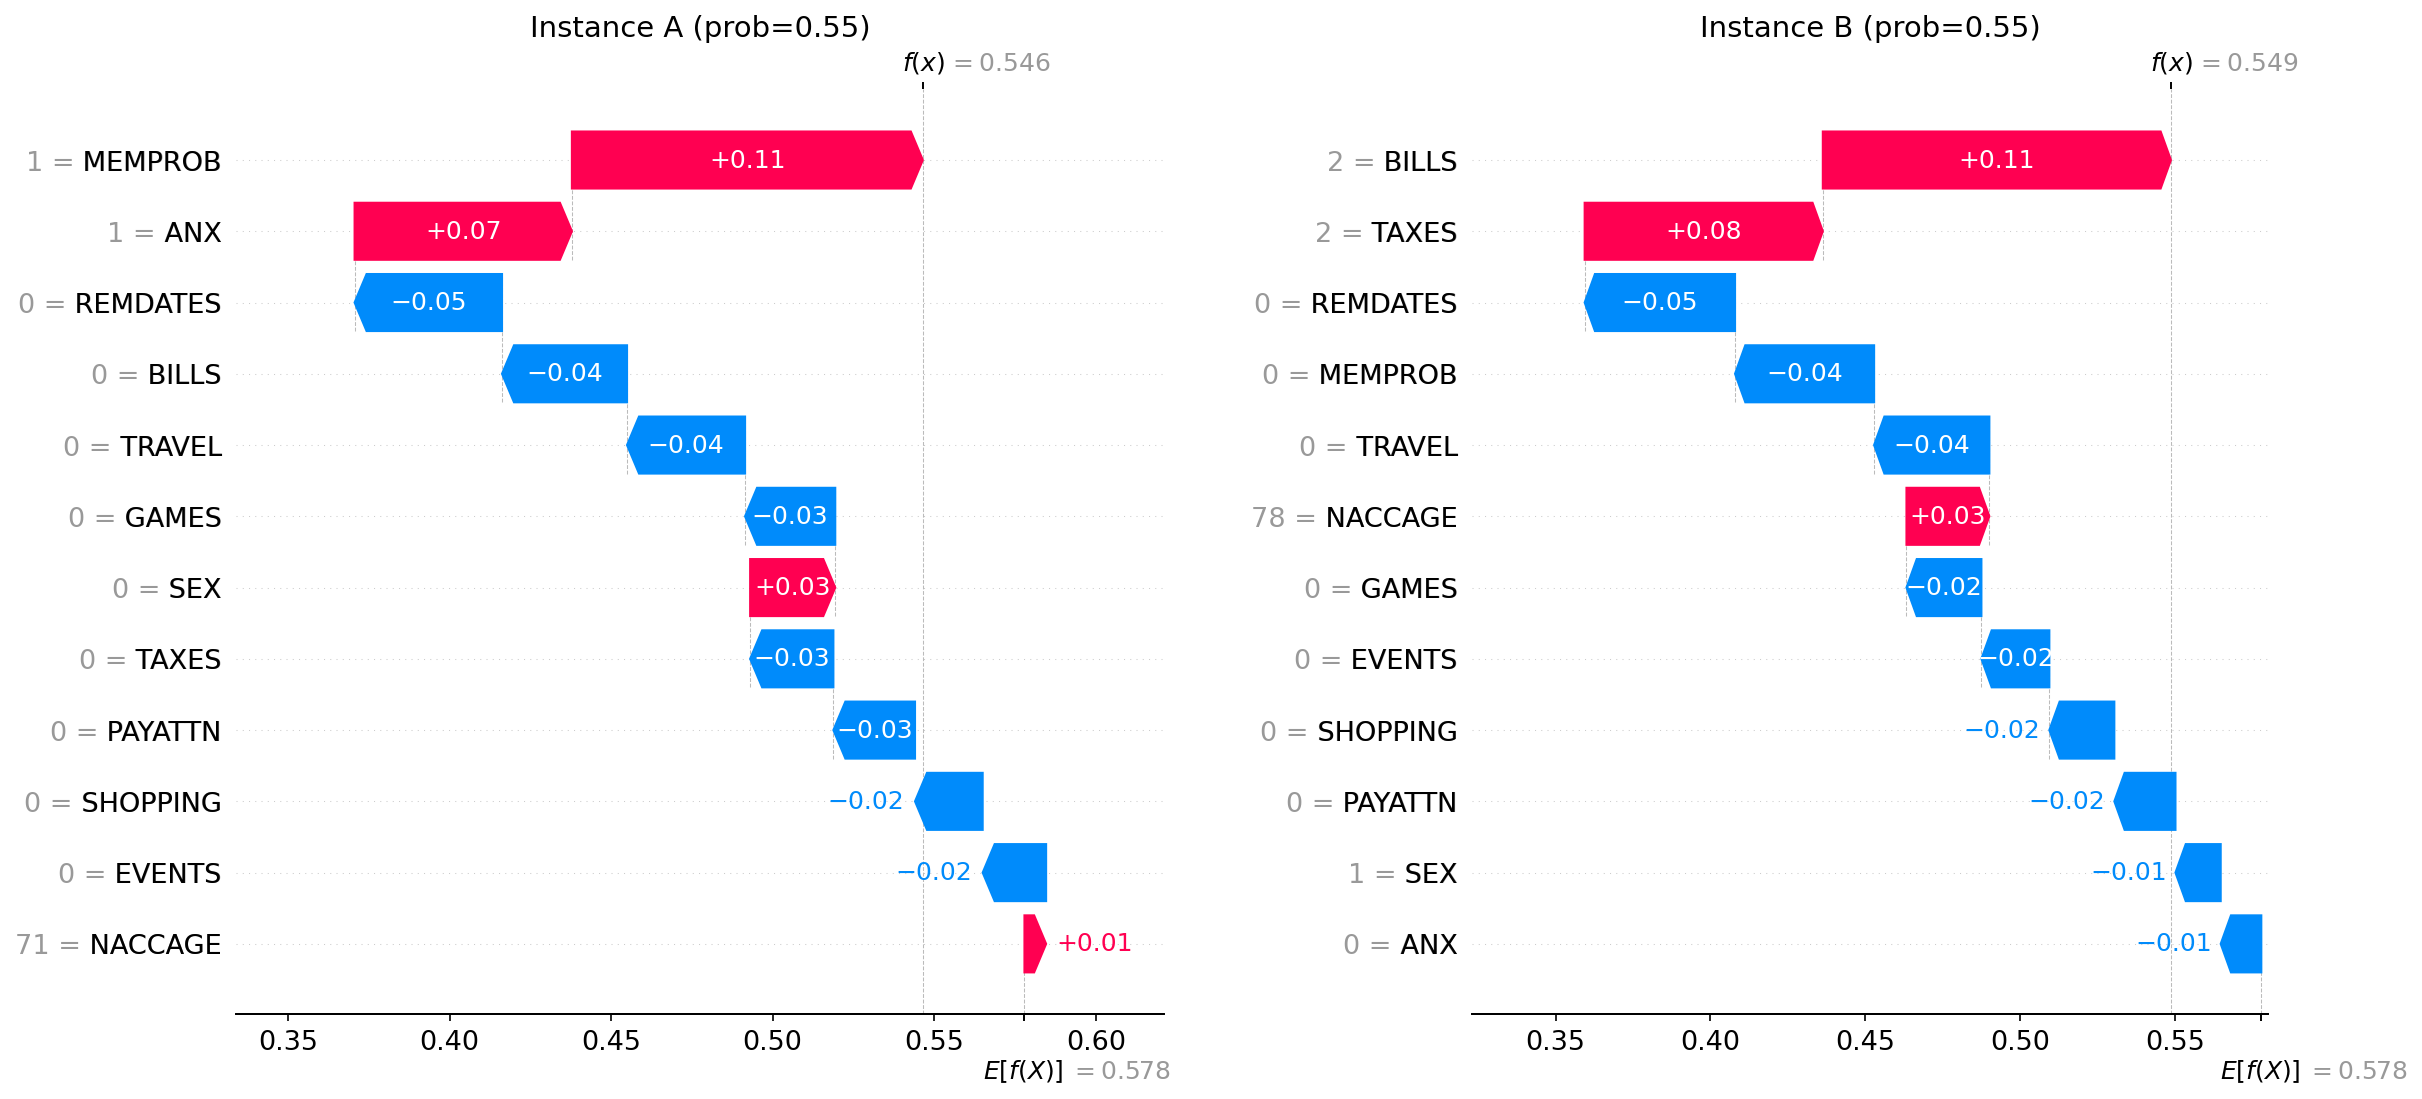
\includegraphics[width=1.0\textwidth]{figures/XAI/impaired_classification_adni_true_positive_waterfall.png}
    \caption{SHAP waterfall plots for two instances correctly classified as cognitive impairment}
    \begin{minipage}{\textwidth}
      \footnotesize \hl{The plot shows how the value of each feature shifts the prediction from the base value to the final predicted probability for a single instance.}
    \end{minipage}
    \label{figure:nc_ci_pos_waterfall}
\end{figure}

Looking at the correctly classified NC instances in Figure~\ref{figure:nc_ci_neg_waterfall}, \textit{Instance A} has a predicted probability of around 44\%. The main reason for classifying this instance as NC is the ability to normally perform most functional activities, pushing the predicted probability 27\% away from CI. This overturned the highest increased risk due to the difficulty in remembering dates and appointments (REMDATES) and the age of 86. On the other hand, \textit{Instance B} represents a male subject who has anxiety and has never paid bills (BILLS). These factors increased his risk of CI compared to \textit{Instance A}. However, \textit{Instance B} was also predicted as NC with a similar probability of around 43\% due to a normal functional profile (including normal REMDATES), normal memory, and younger age than \textit{Instance A}.

\begin{figure}[ht]
    \centering
    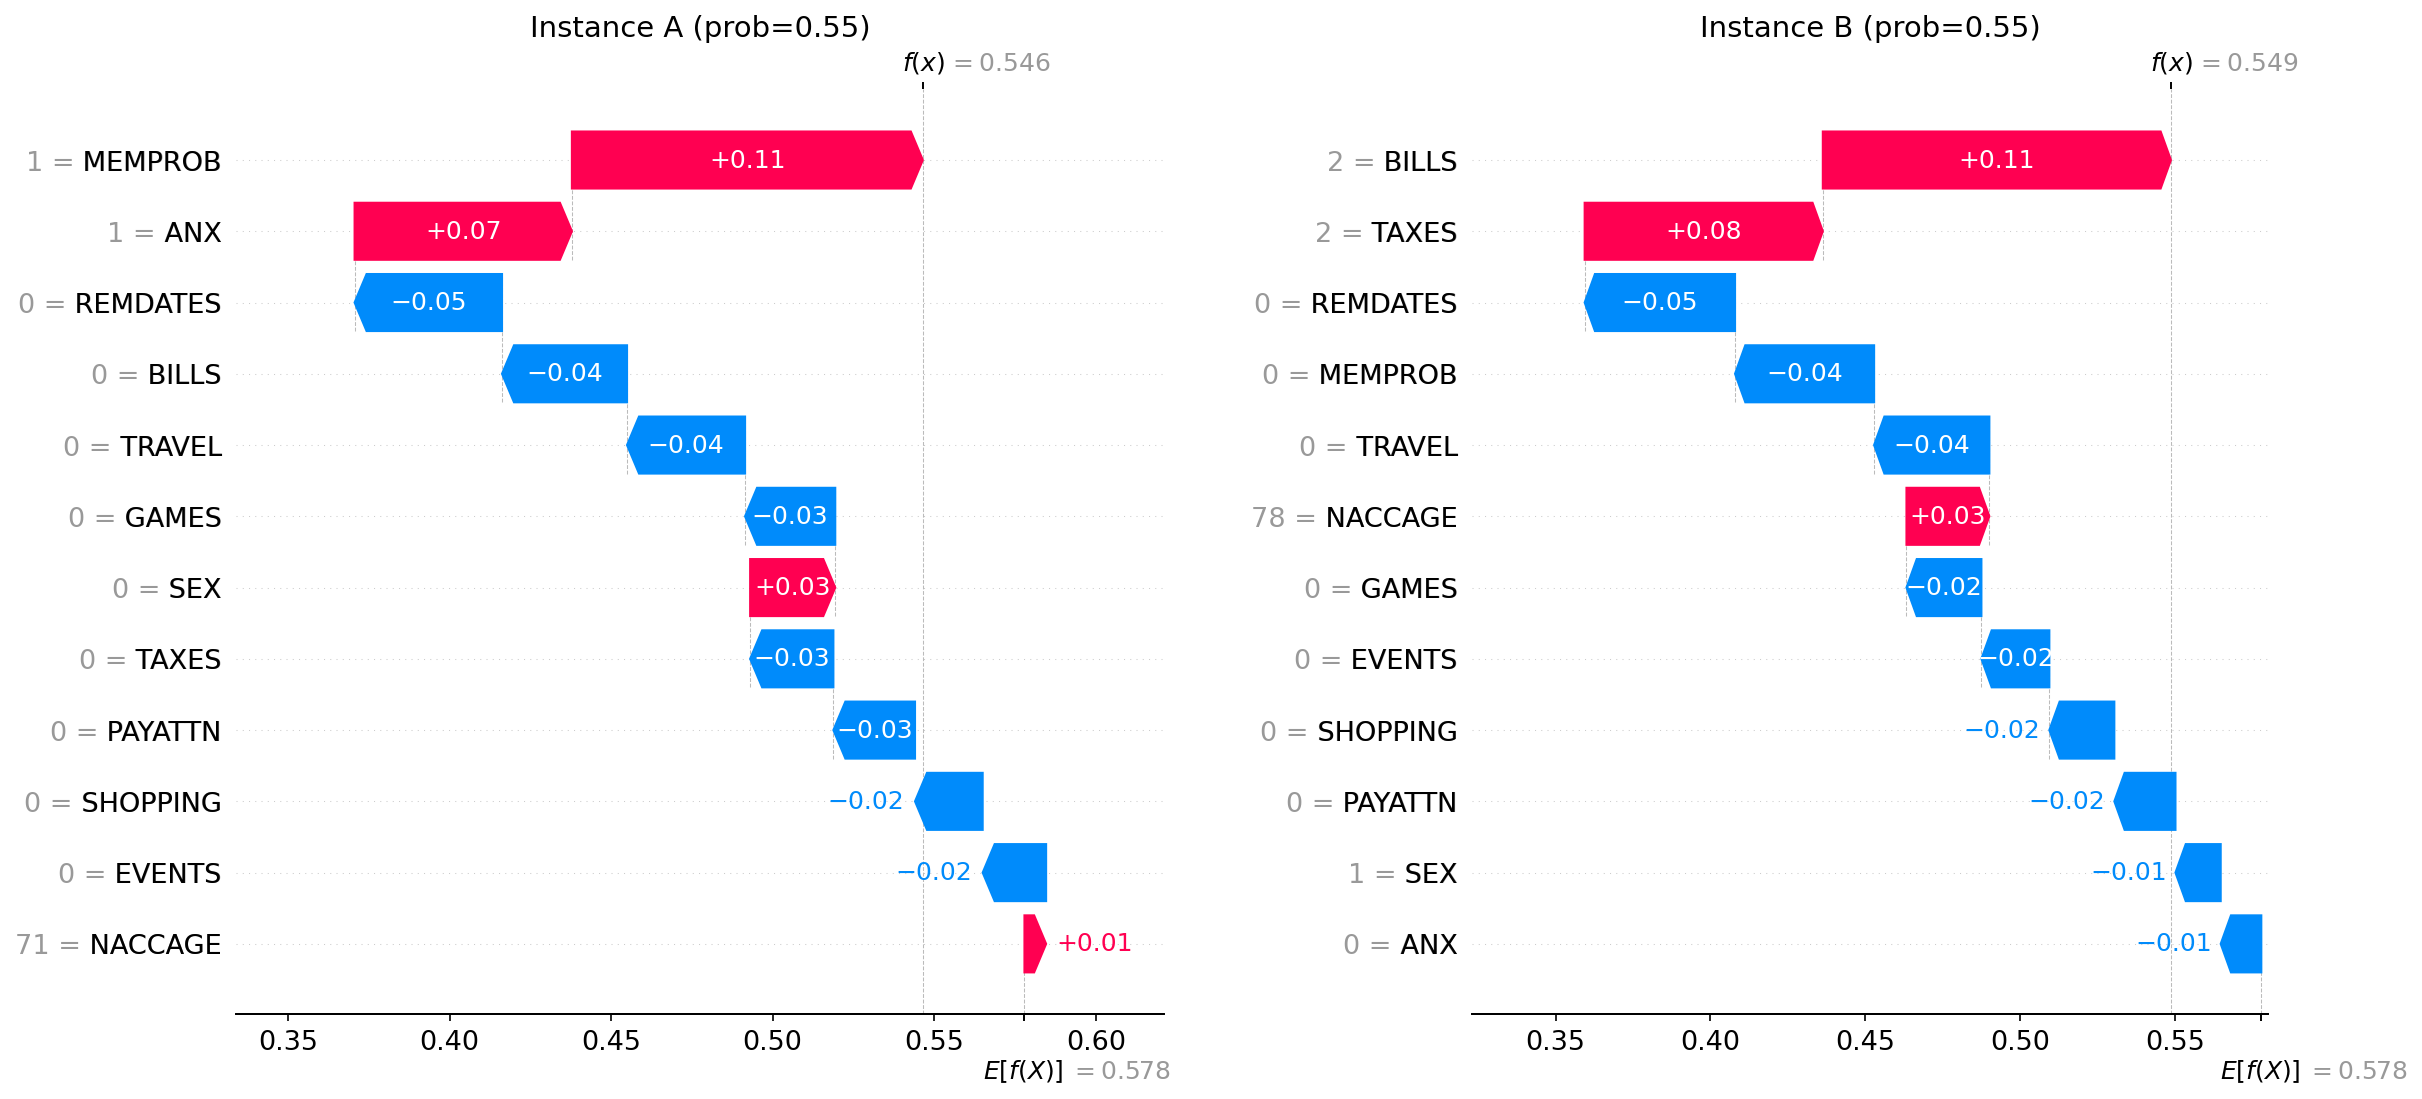
\includegraphics[width=1.0\textwidth]{figures/XAI/impaired_classification_adni_true_positive_waterfall.png}
    \caption{SHAP waterfall plots for two instances correctly classified as normal cognition}
    \begin{minipage}{\textwidth}
      \footnotesize \hl{The plot shows how the value of each feature shifts the prediction from the base value to the final predicted probability for a single instance.}
    \end{minipage}
    \label{figure:nc_ci_neg_waterfall}
\end{figure}

The analysis of the counterfactual explanation performed by Diverse Counterfactual Explanations (\acrshort{DiCE}) is shown in Figure~\ref{figure:nc_ci_dice_stat}. DiCE was able to generate at least one counterfactual example for approximately 99\% of the ADNI samples (mean = 2.66, median = 2). Most instances had more than one suggestion for risk intervention (counterfactual examples), while only about 11\% of instances had up to five counterfactual examples.

\begin{figure}[ht]
    \centering
    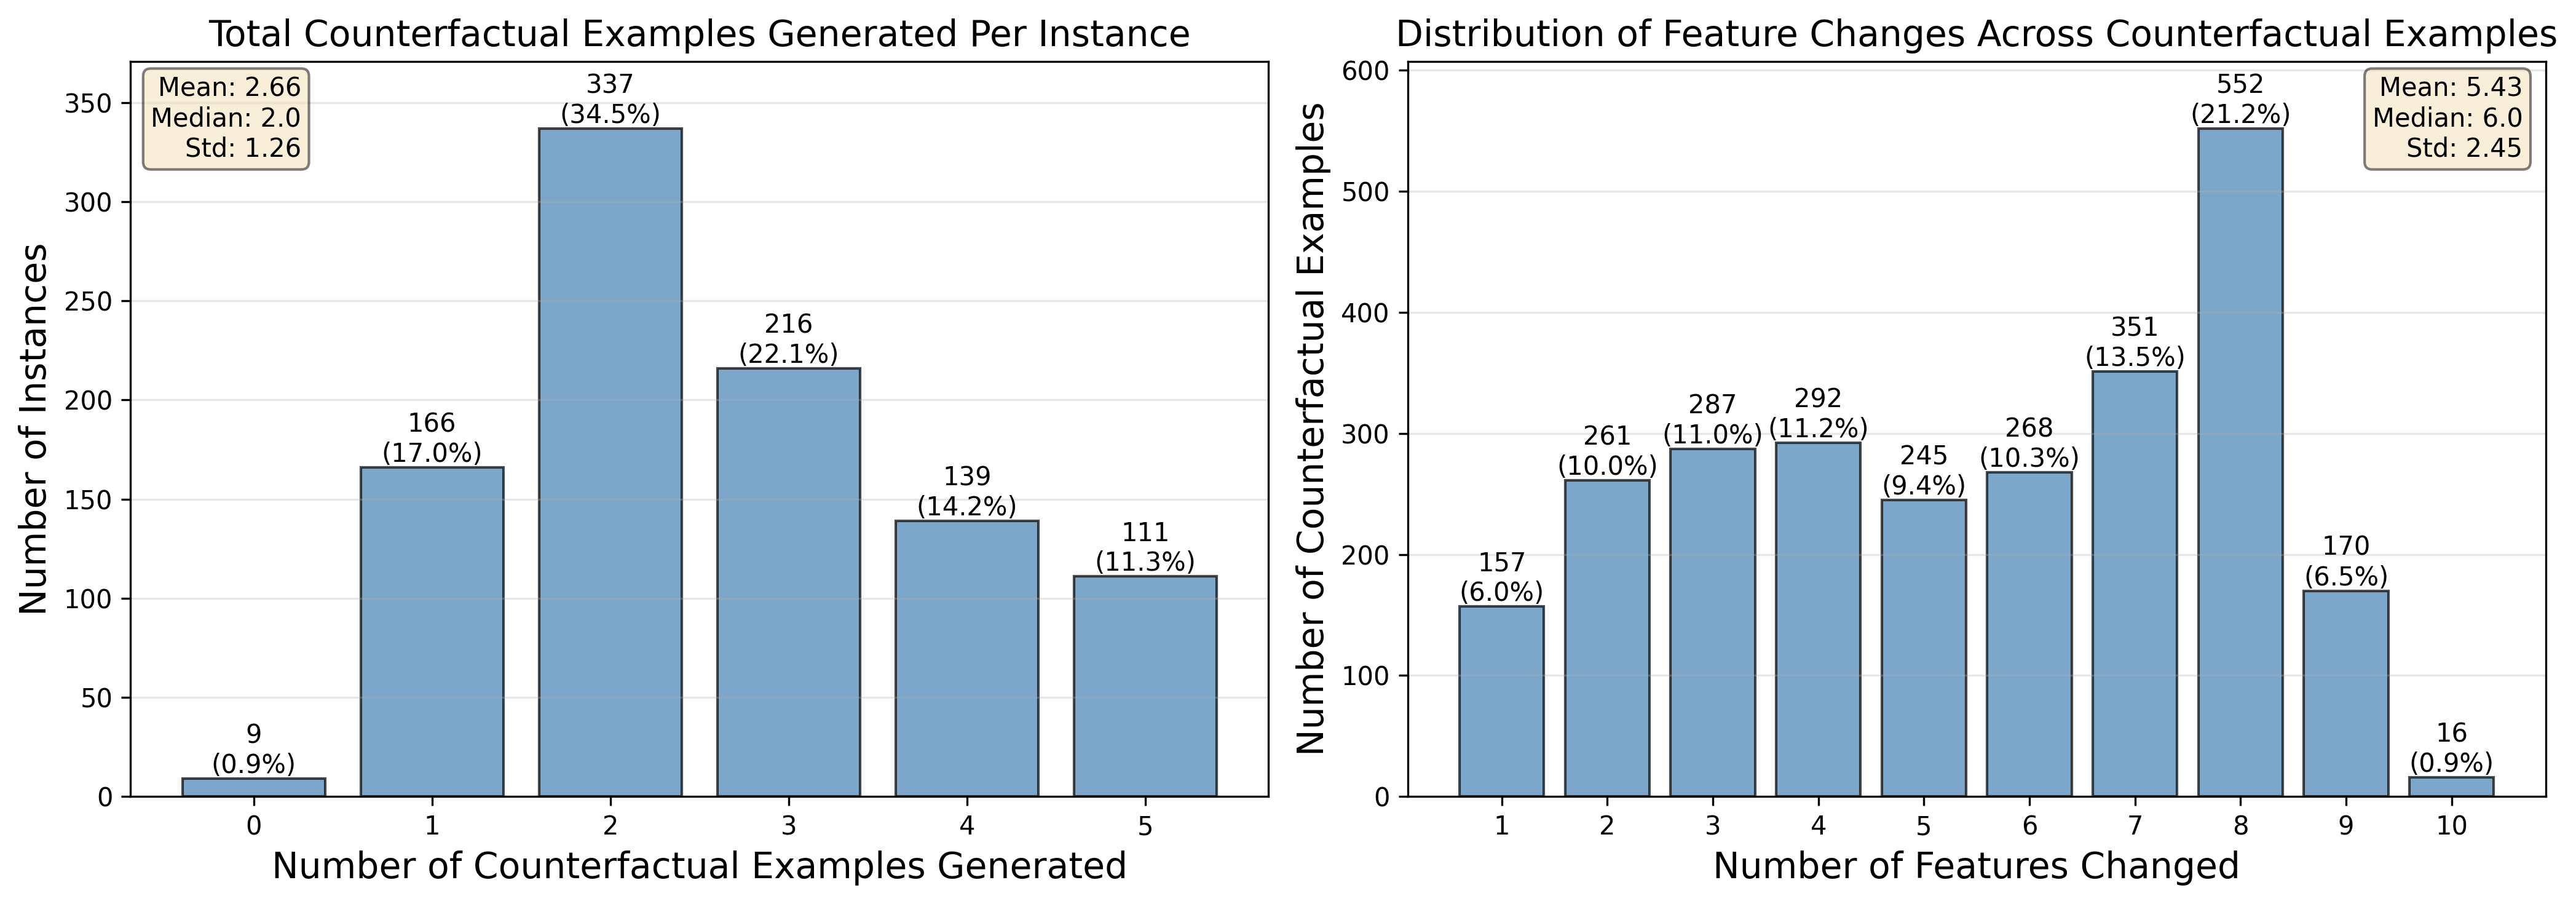
\includegraphics[width=1.0\textwidth]{figures/XAI/impaired_classification_adni_kdtree_dice_stats.png}
    \caption{Summary of generated counterfactual examples for changing the model classification from cognitive impairment to normal cognition}
    \label{figure:nc_ci_dice_stat}
\end{figure}

As shown in the right chart of Figure~\ref{figure:nc_ci_dice_stat}, of the 10 modifiable features, on average about 5 to 6 features needed to be changed to generate valid counterfactuals. The majority of counterfactual examples required modifying between 2 and 9 features, with the highest frequency being 8 features (21.2\%). A very small percentage of counterfactual examples required altering all 10 features. Similar results were observed in the counterfactual explanation of the NACC cross-center validation dataset which can be found in Figure~\ref{figure:dice-nacc-task1-apdx} in the appendix.

The most effective features for risk interventions can be analyzed using the feature importance bar chart in Figure~\ref{figure:nc_ci_dice_feature_importance}. Functional activities related to FAQ were the most frequently modified features. The top three features are handling taxes (76\%), remembering dates (74\%), and paying bills (71\%). In contrast, reported memory problems (MEMPROB) and anxiety (ANX) were less frequently changed, with scores of 17\% and 32\%, respectively. Table~\ref{table:cfe-adni-task1-apdx} in the appendix illustrates counterfactual examples generated for a random subject classified as CI to reverse the estimated outcome to NC.

\begin{figure}[ht]
    \centering
    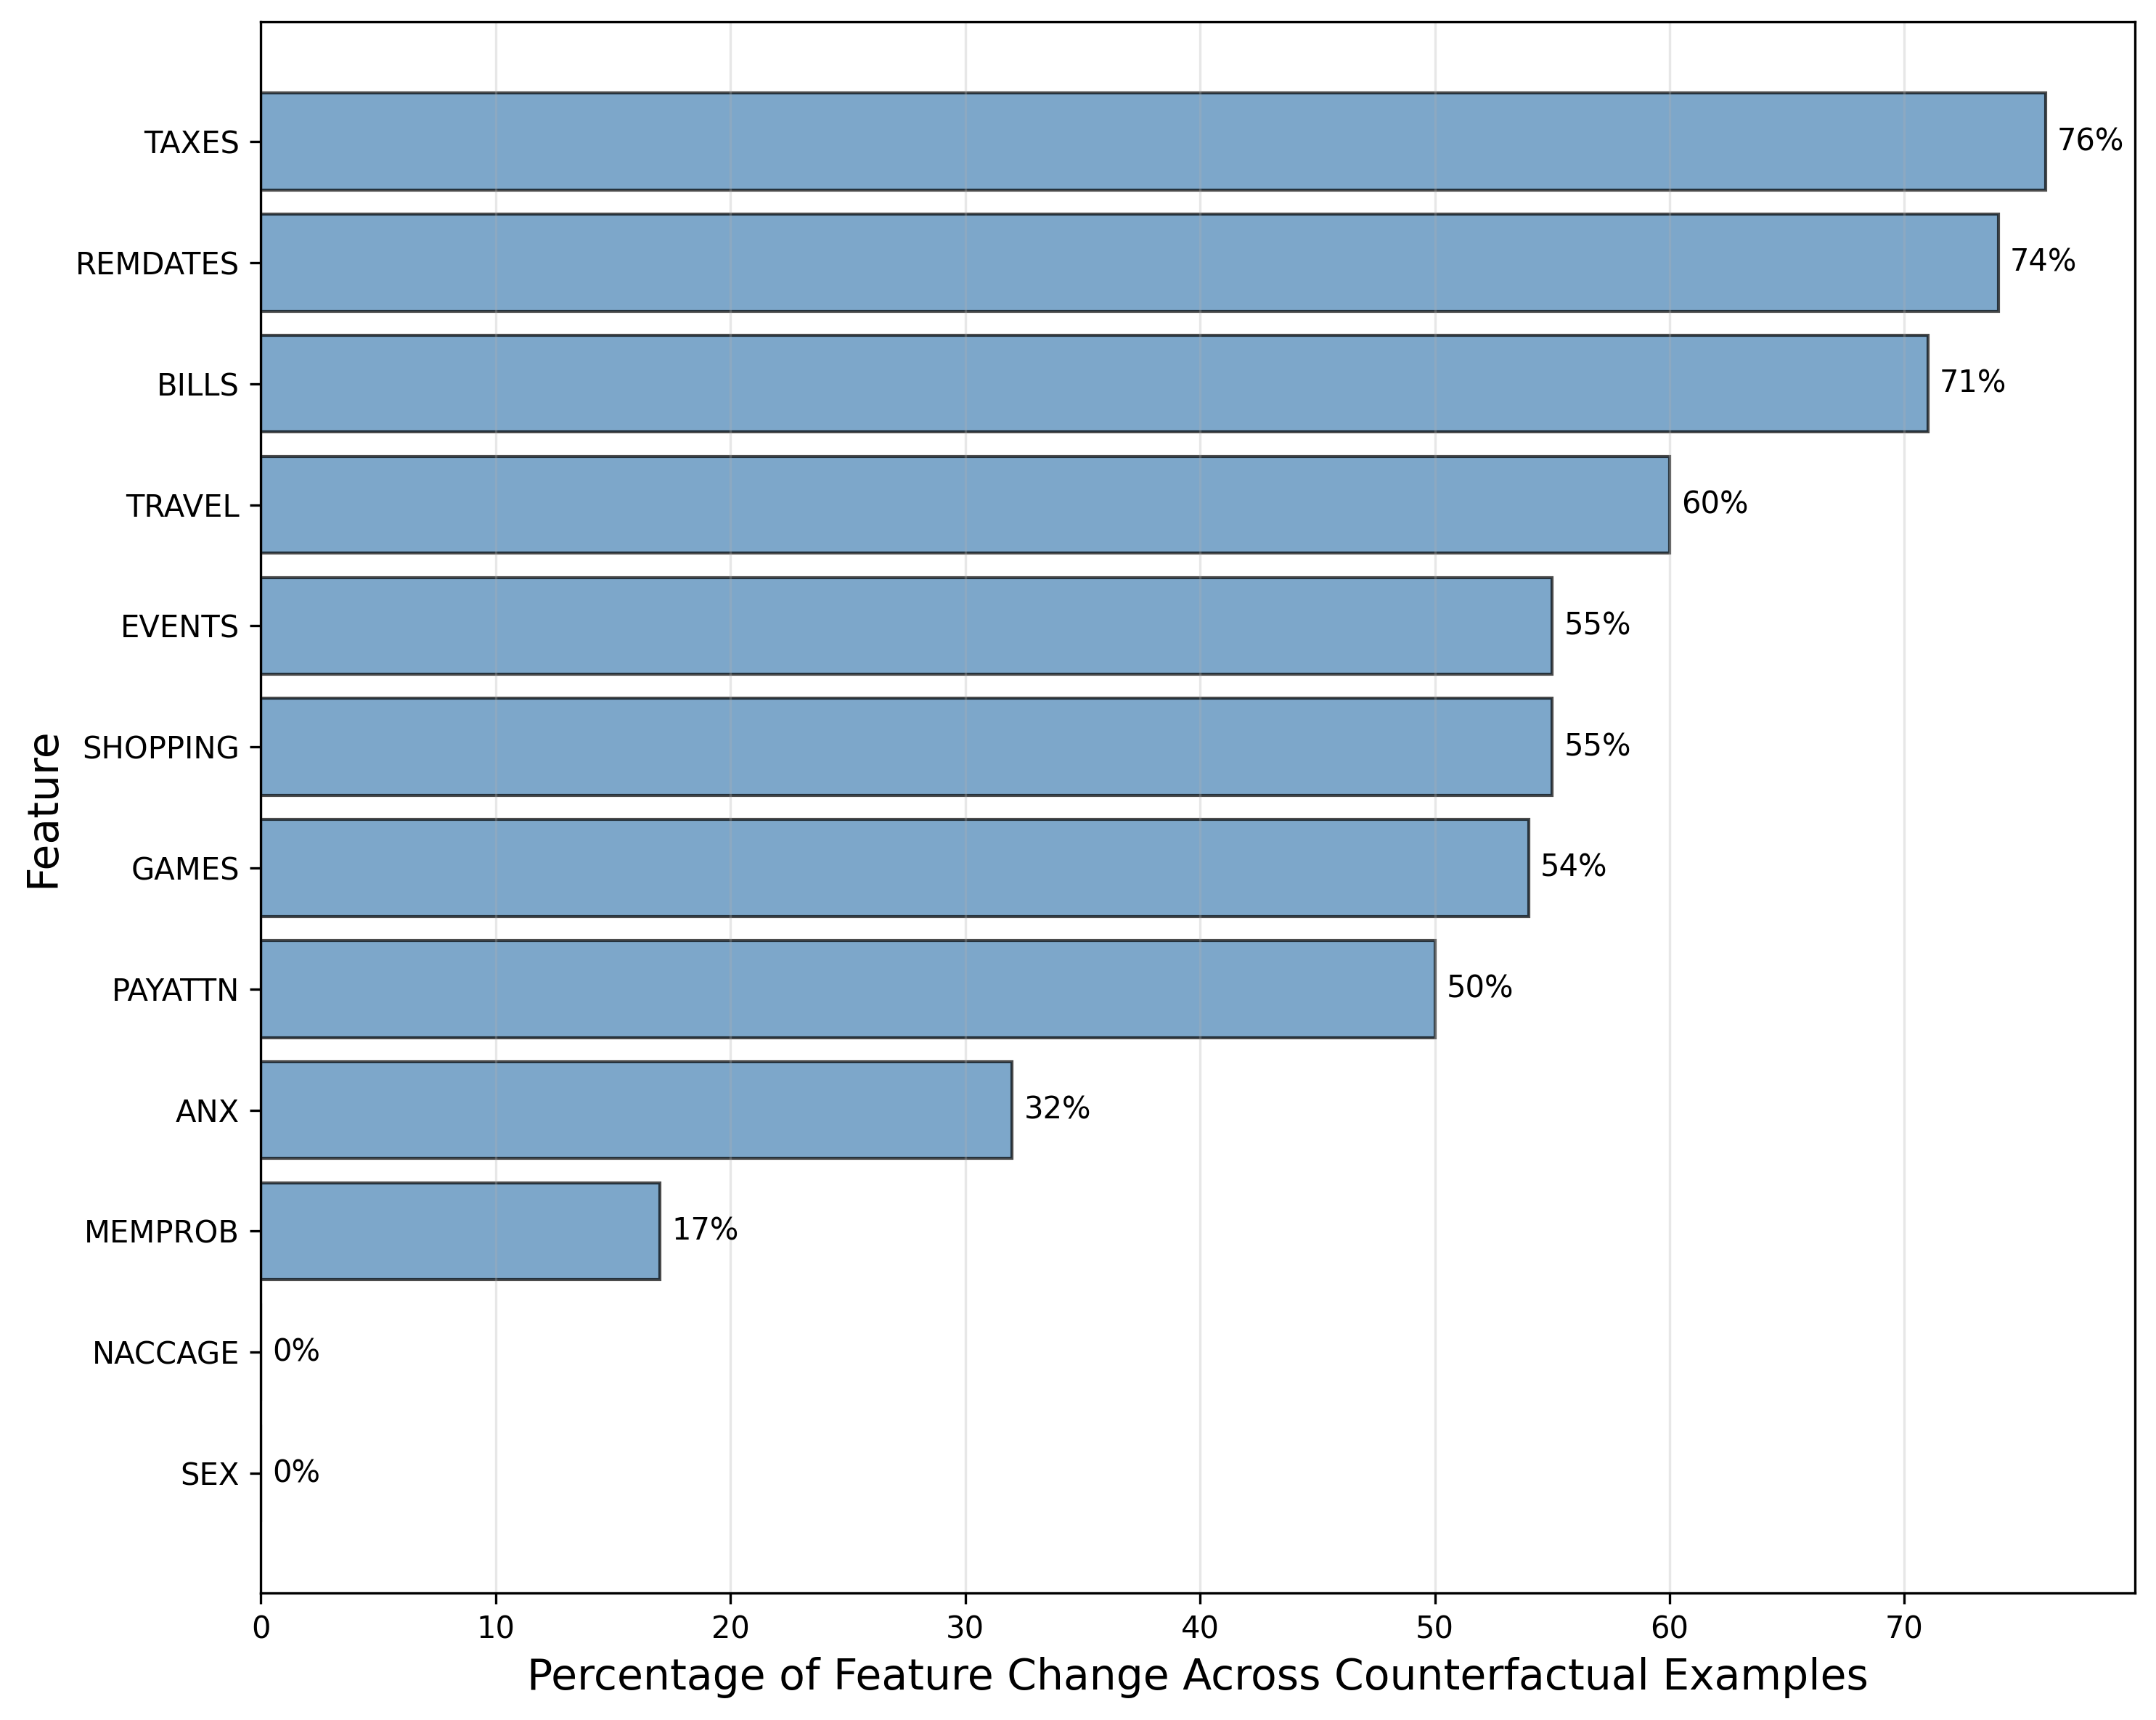
\includegraphics[width=1.0\textwidth]{figures/XAI/impaired_classification_adni_kdtree_dice_global_importance.png}
    \caption{Feature importance ranking based on counterfactual explanations for the NC vs. CI classification task}
    \begin{minipage}{\textwidth}
      \footnotesize The features are ranked based on the percentage of times they were modified to generate valid counterfactual examples. The rank highlights the most critical features for risk intervention. Demographic features (NACCAGE and SEX) show 0\% importance because they were set as invariable features in the counterfactual generation process.
    \end{minipage}
    \label{figure:nc_ci_dice_feature_importance}
\end{figure}

\subsubsection{Model Explainability Results for the CIND vs. Dementia Classification Task}
The global feature importance ranking for the CIND vs. dementia classification task is presented in Figure~\ref{figure:cind_dementia_feature_importance}. The figure shows the mean absolute SHAP values of the features in both the NACC cross-center validation and the ADNI external validation. The Spearman’s rank correlation coefficient of 0.98 ($p$ < 0.05) demonstrates a high degree of consistency in the ranking of feature importance between these two external validation datasets. Similarly to the NC vs. CI classification tasks, functional activity features emerged as the dominant factors influencing the model's predictions in both external validation datasets. The three most important predictors are BILLS, TRAVEL, and EVENTS. In contrast, features such as primary language (PRIMLANG) and changes of appetite (APP) consistently showed a lower importance. 

\begin{figure}[ht]
    \centering
    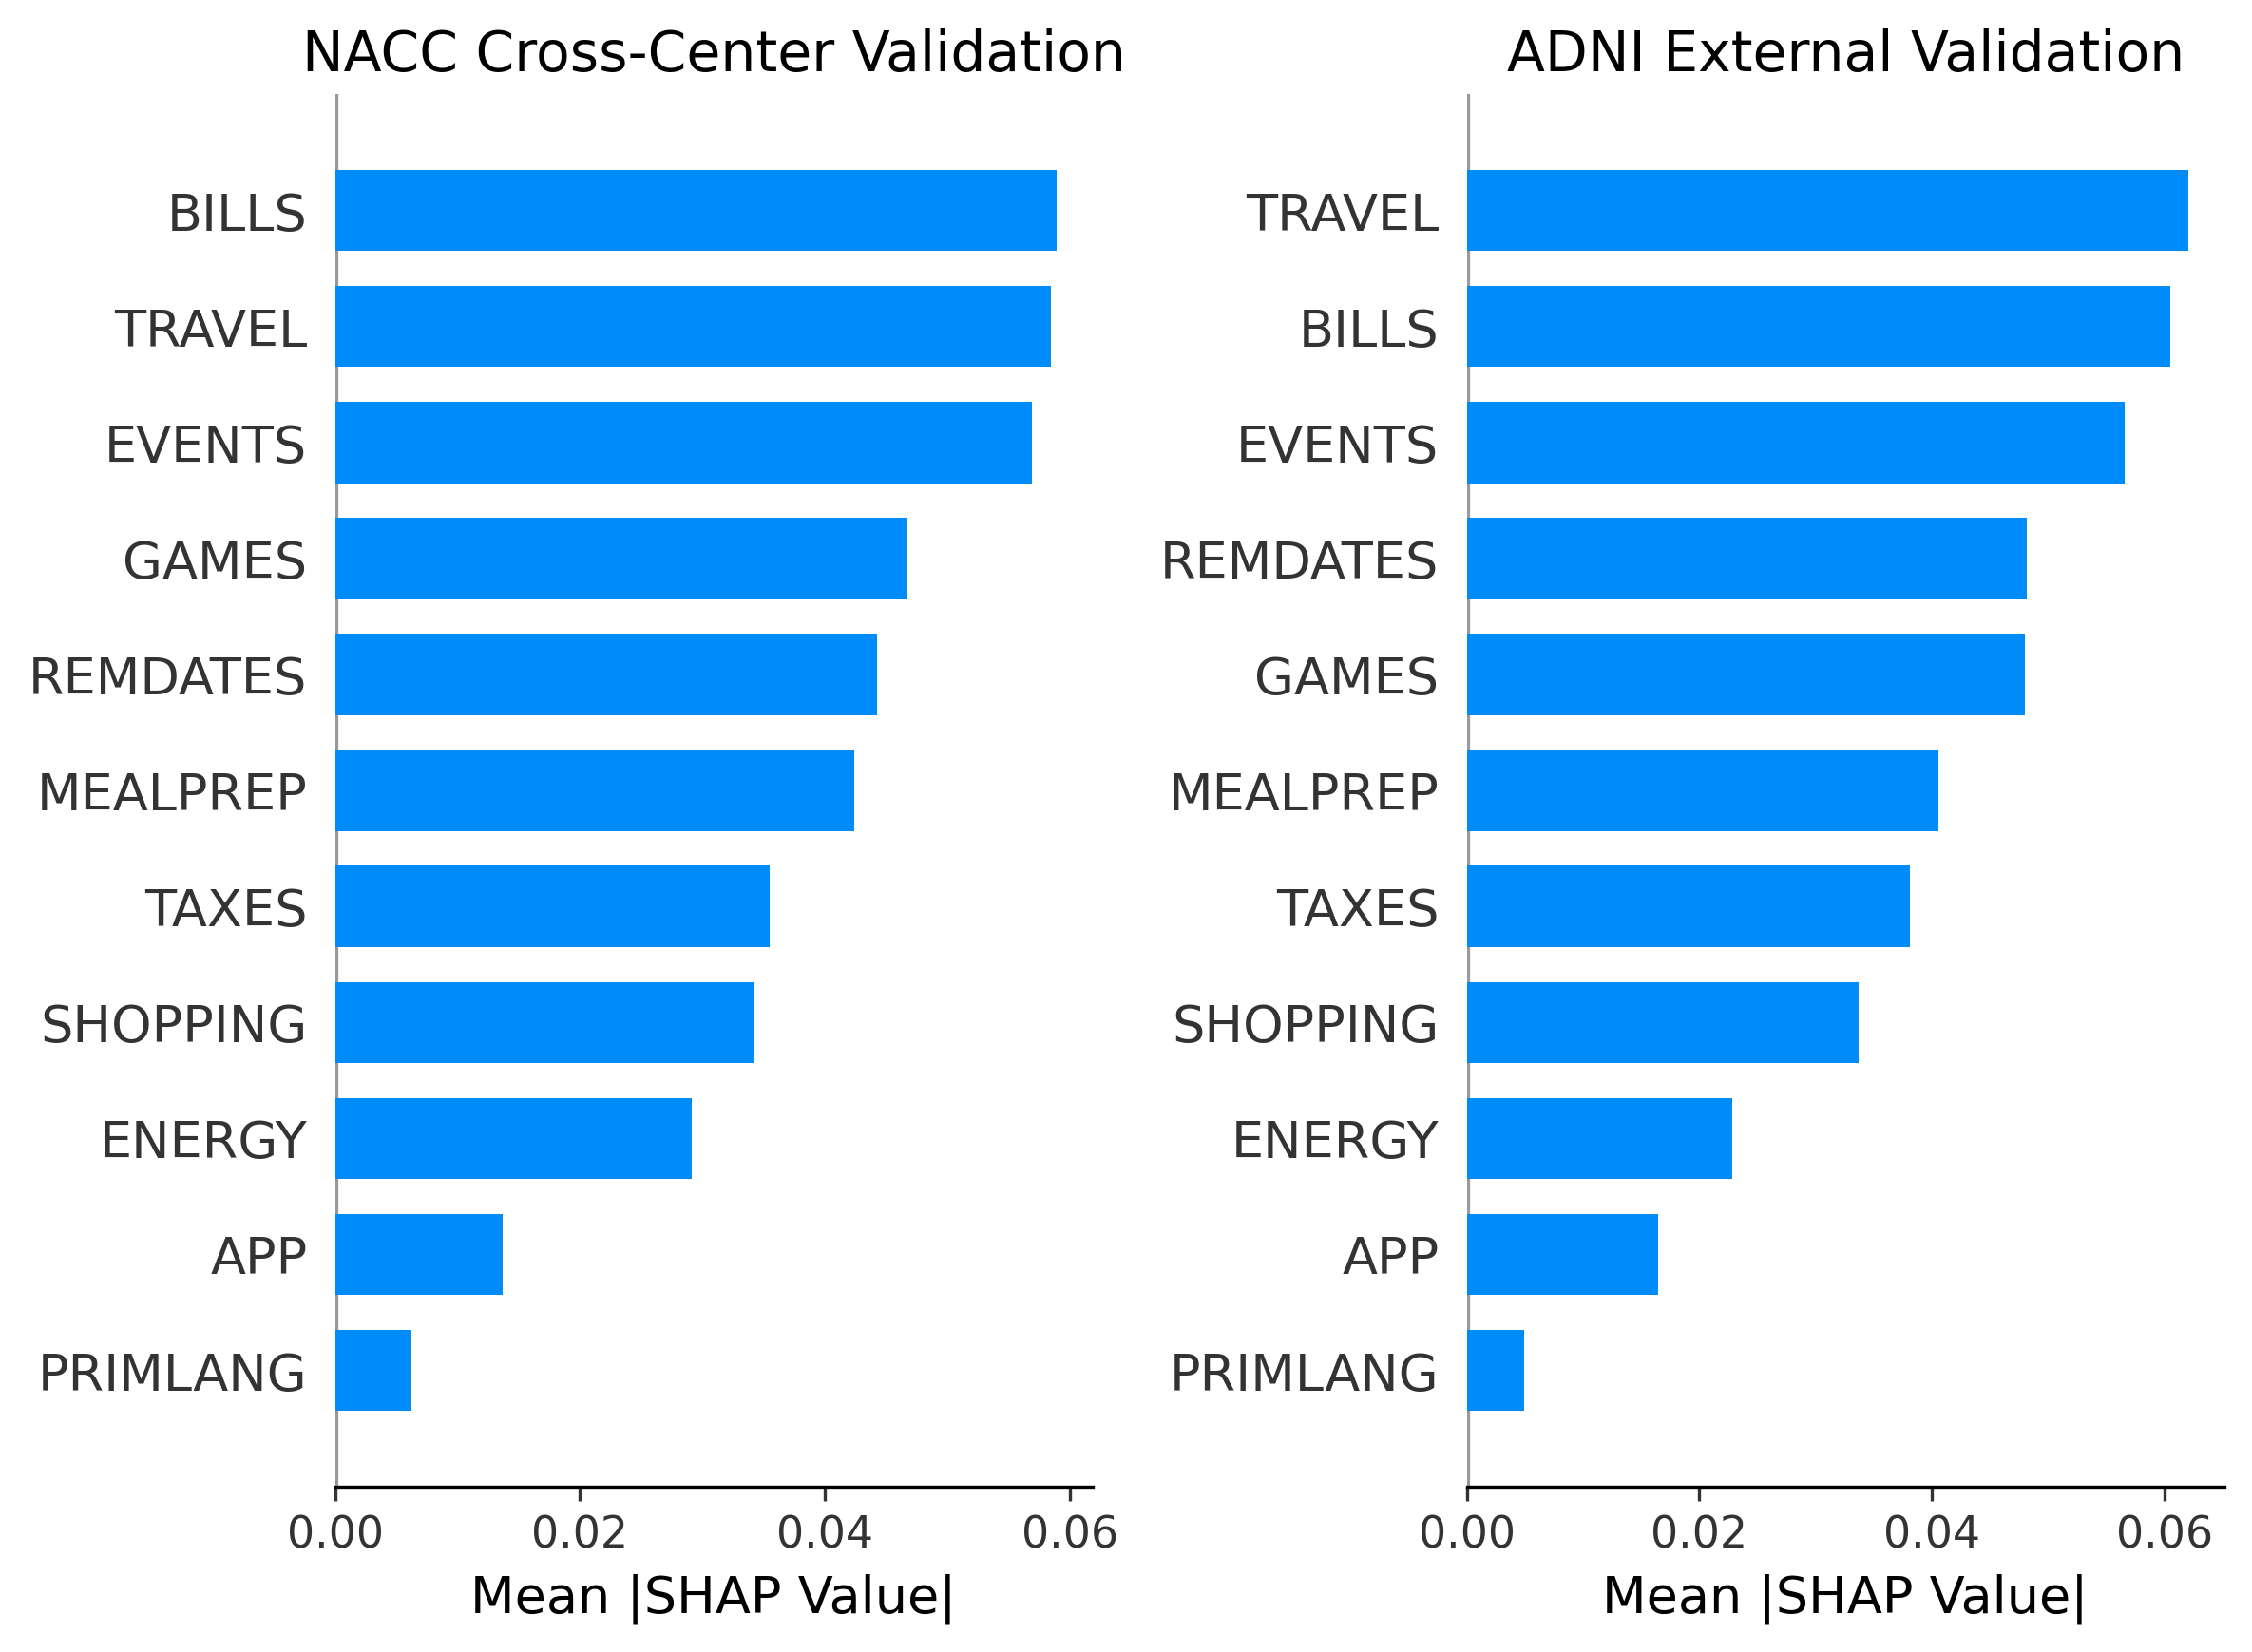
\includegraphics[width=1.0\textwidth]{figures/XAI/dementia_classification_both_feature_importance_comparison.png}
    \caption{Feature importance in the NACC cross-center validation and the ADNI external validation for the CIND vs. dementia classification task}
    \begin{minipage}{\textwidth}
      \footnotesize \hl{The bars represent the mean absolute SHAP value of each feature, which ranks the contribution of the feature to the model prediction in the two validation datasets.}
    \end{minipage}
    \label{figure:cind_dementia_feature_importance}
\end{figure}

To evaluate the local explanation of the model, two correctly classified instances from each class with distinct feature profiles have been analyzed to demonstrate the model's ability to capture heterogeneous patterns. For instances classified as dementia, both \textit{Instance A} and \textit{Instance B} in Figure~\ref{figure:cind_dementia_pos_waterfall} had similar predicted probabilities of approximately 58\% and 57\%, respectively. However, both instances have different contributing factors. \textit{Instance A} requires assistance with filling taxes (TAXES) and has difficulty tracking current events (EVENTS), in addition to reported appetite changes (APP). In contrast, \textit{Instance B} presented a different functional decline profile, as it requires assistance with traveling (TRAVEL) and remembering dates (REMDATES).

\begin{figure}[ht]
    \centering
    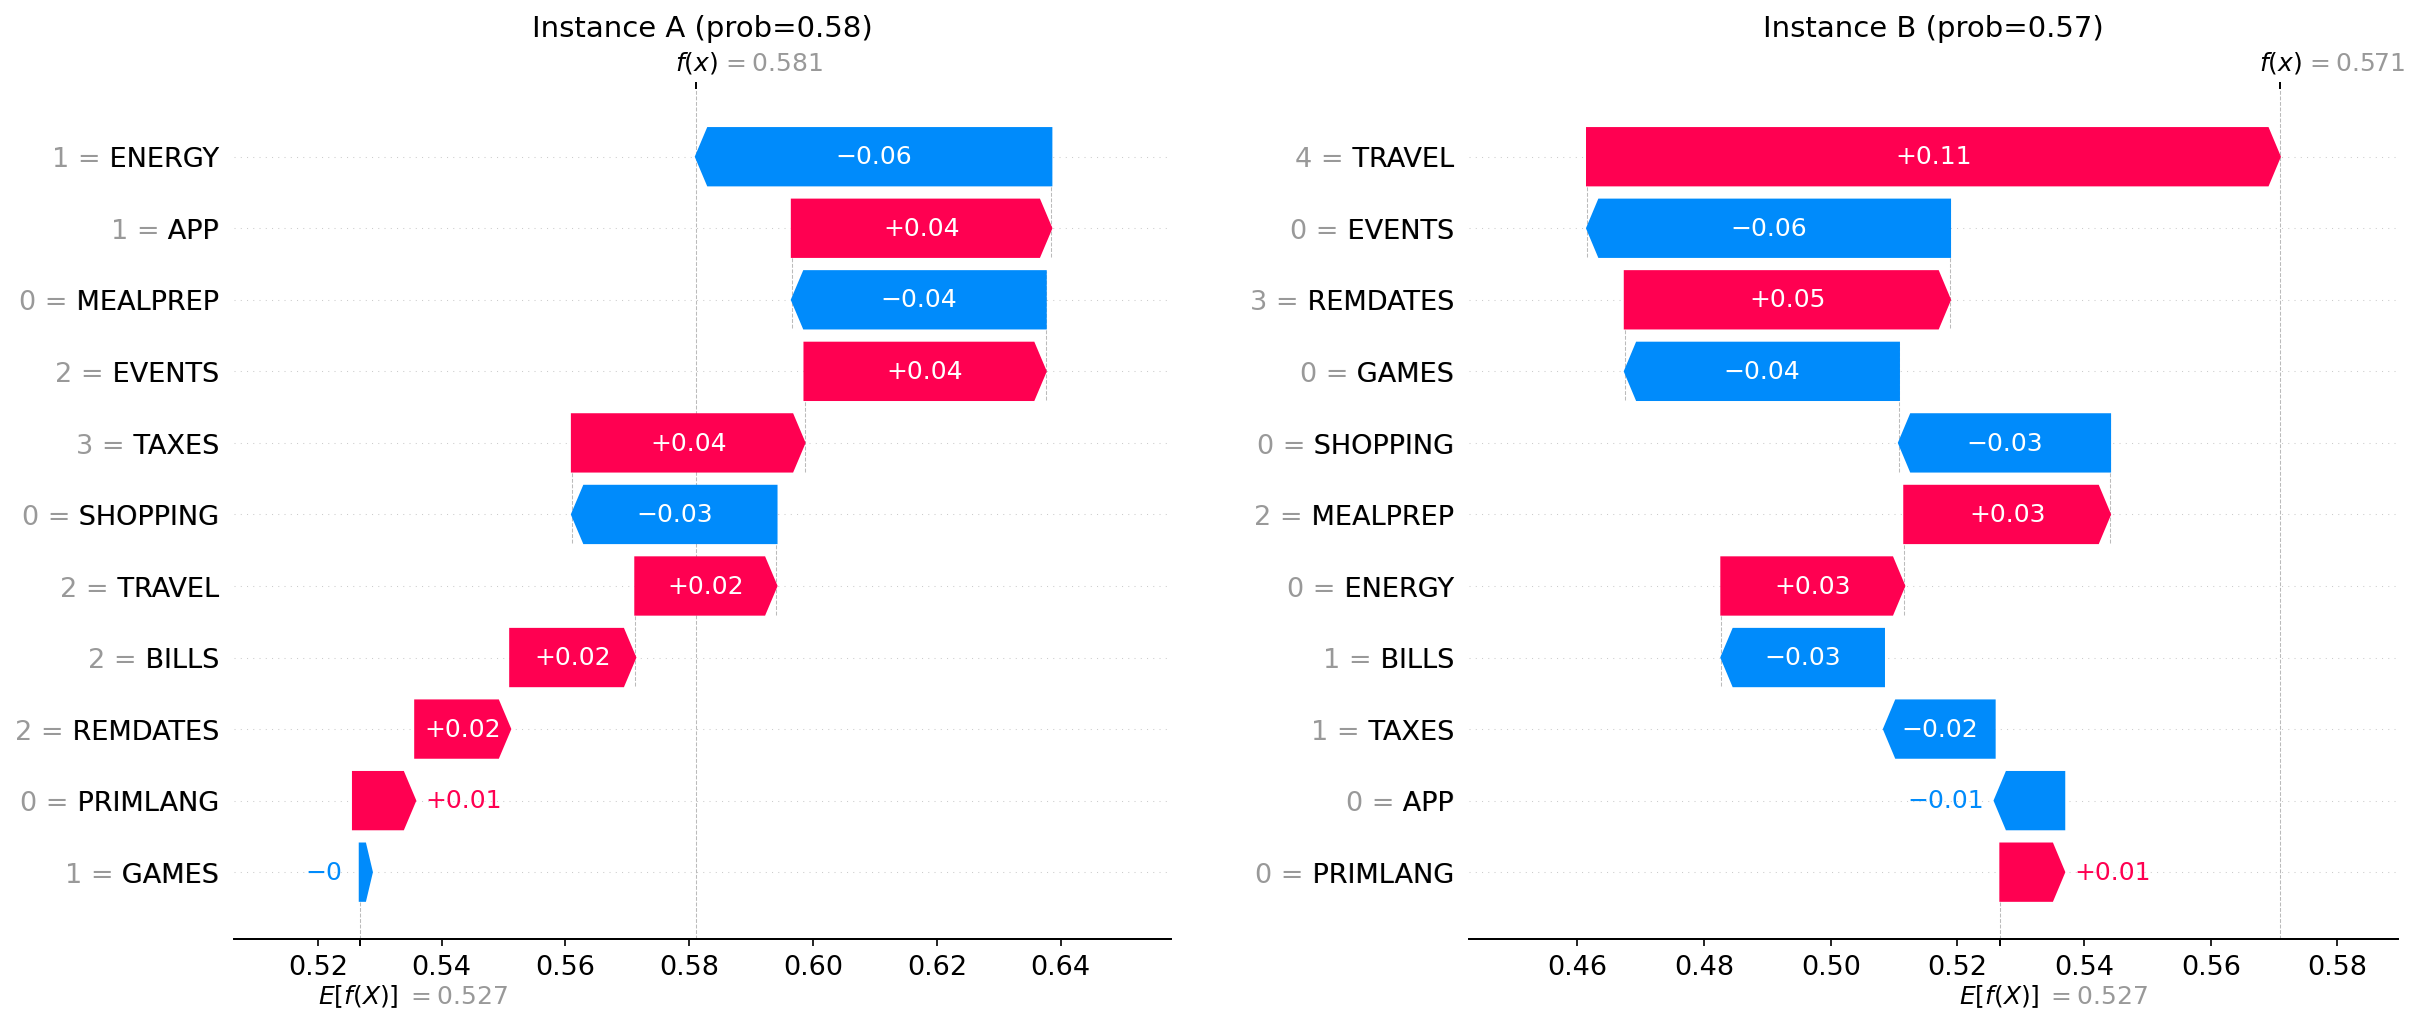
\includegraphics[width=1.0\textwidth]{figures/XAI/dementia_classification_adni_true_positive_waterfall.png}
    \caption{SHAP waterfall plots for two instances correctly classified as dementia}
    \begin{minipage}{\textwidth}
      \footnotesize \hl{The plot shows how the value of each feature shifts the prediction from the base value to the final predicted probability for a single instance.}
    \end{minipage}
    \label{figure:cind_dementia_pos_waterfall}
\end{figure}

The other two randomly selected CIND instances in Figure~\ref{figure:cind_dementia_neg_waterfall} were classified with probabilities of 40\%. \textit{Instance A} represented a profile of functional independence, with the ability to normally handle bills, taxes, events, and meal preparation. This level of independence was strong enough to minimize the risk of dementia introduced by appetite changes and other risk factors. With a different pattern, the classification of \textit{Instance B} as CIND was driven by the ability to normally track events and remember dates regardless of the difficulty in handling financial tasks.

\begin{figure}[ht]
    \centering
    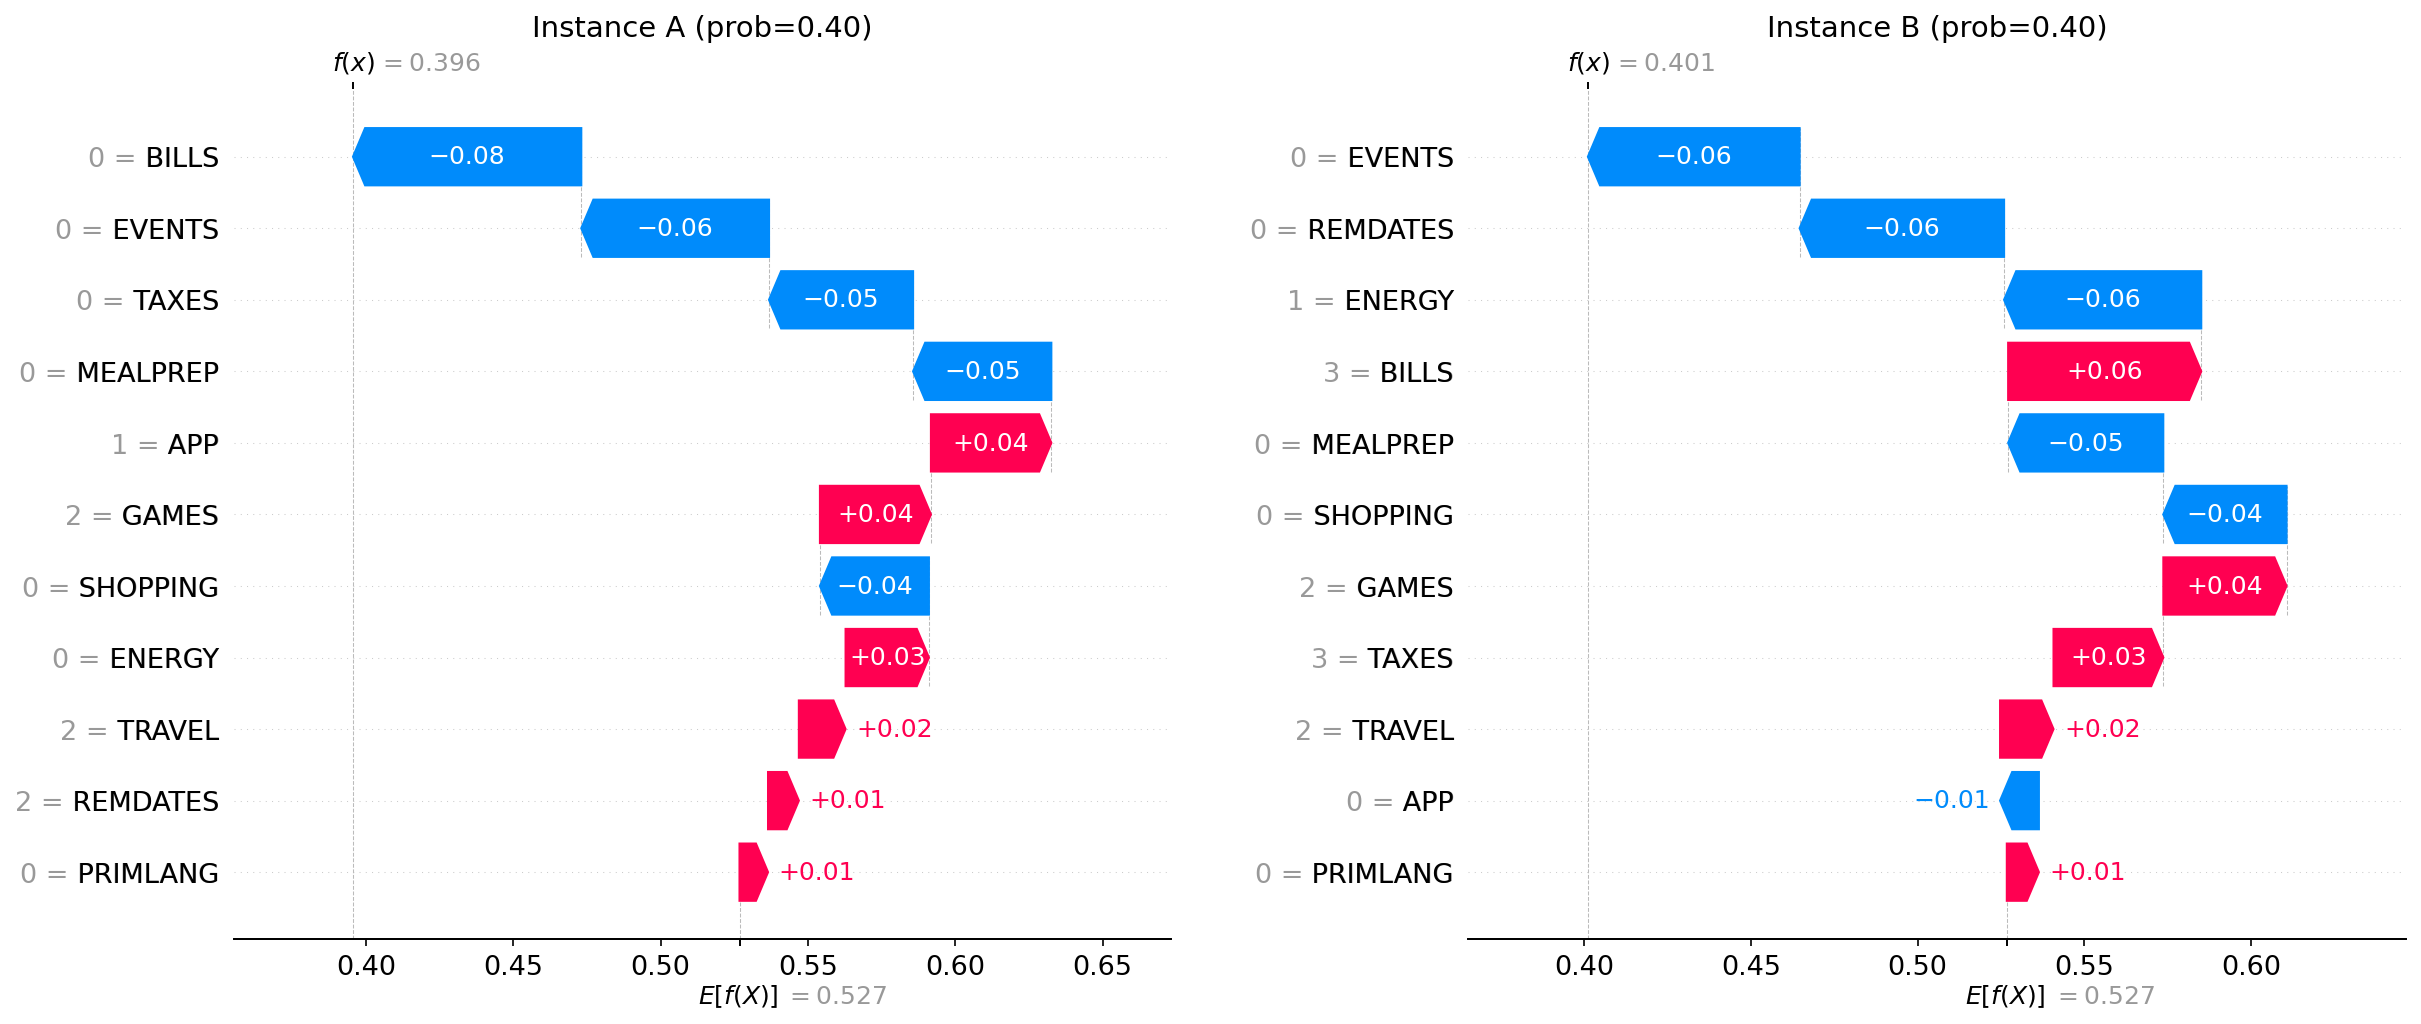
\includegraphics[width=1.0\textwidth]{figures/XAI/dementia_classification_adni_true_negative_waterfall.png}
    \caption{SHAP waterfall plots for two instances correctly classified as cognitive impairment but not dementia (CIND)}
    \begin{minipage}{\textwidth}
      \footnotesize \hl{The plot shows how the value of each feature shifts the prediction from the base value to the final predicted probability for a single instance.}
    \end{minipage}
    \label{figure:cind_dementia_neg_waterfall}
\end{figure}

In regard to the results of the counterfactual explanation in the ADNI external validation, counterfactual examples were generated for more than 91\% of the instances (mean = 4.38, median = 5). The majority of instances (83.6\%) had five counterfactual examples generated, while only 8.6\% of the instances had no counterfactual examples found. The analysis of the counterfactual explanation performed by the DiCE method is shown in Figure~\ref{figure:cind_dementia_dice_stat}.

\begin{figure}[ht]
    \centering
    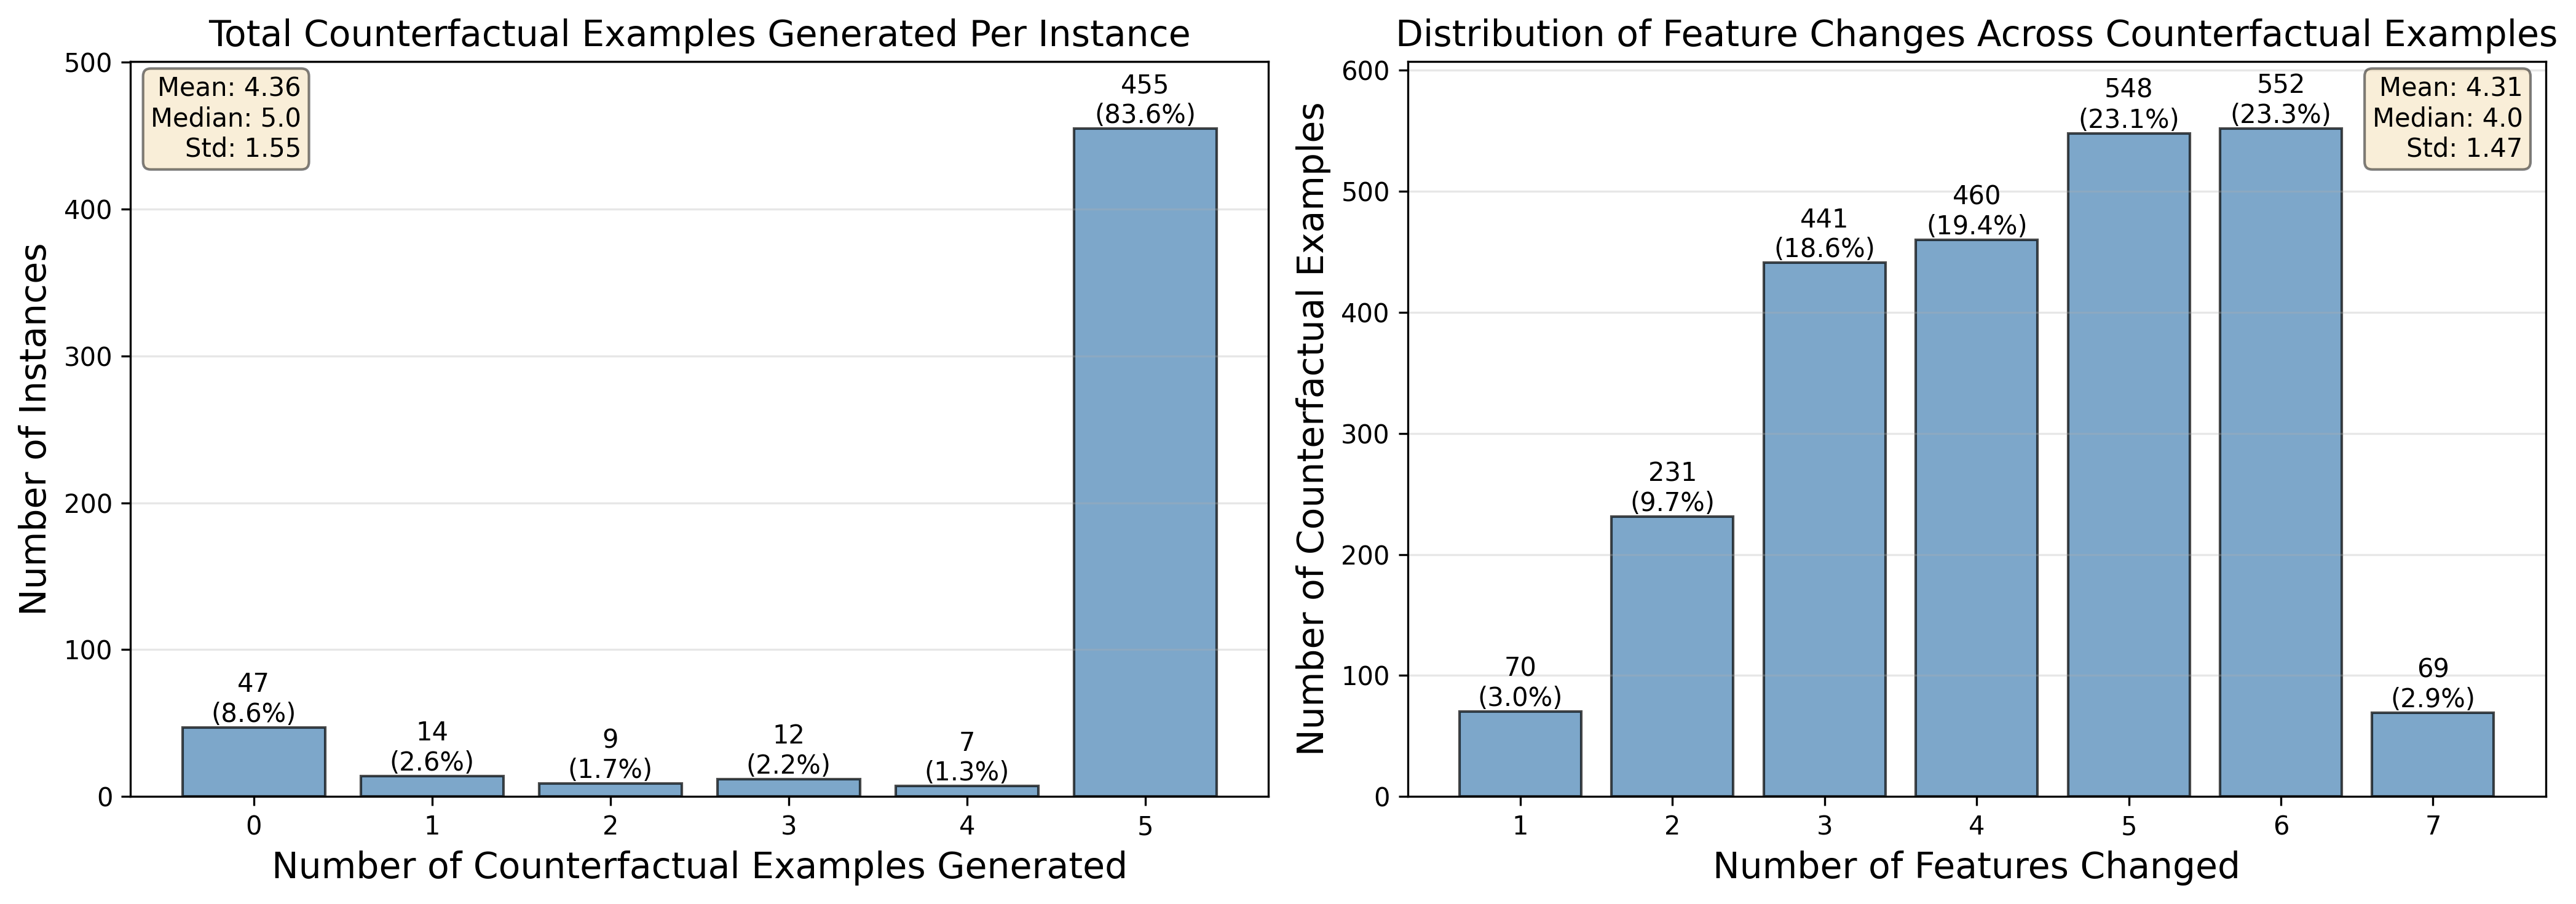
\includegraphics[width=1.0\textwidth]{figures/XAI/dementia_classification_adni_kdtree_dice_stats.png}
    \caption{Summary of generated counterfactual examples for changing the model classification from dementia to CIND}
    \label{figure:cind_dementia_dice_stat}
\end{figure}

Analyzing the changes in the features revealed that, on average, approximately 4 out of the 11 features needed to be changed to generate valid counterfactuals. The effort required for risk intervention is moderate, with the majority of counterfactual examples generated by modifying between 3 and 6 features. A minimal percentage of examples required altering only 1 feature (3\%) or up to 7 features (2.9\%). Interestingly, no counterfactual examples required changes of more than 7 features. The counterfactual explanation of the NACC cross-center validation dataset, presented in Figure~\ref{figure:dice-nacc-task2-apdx} in the appendix, resulted in similar outcomes.

The bar chart in Figure~\ref{figure:cind_dementia_dice_feature_importance} presents the frequency of changes in each feature to generate counterfactual examples. Functional activities related to daily living were the most frequently modified features to reverse the risk of dementia. The top five features are preparing balanced meals (MEALPREP, 61\%), tracking current events (EVENTS, 58\%), playing games of skill (GAMES, 54\%), shopping (SHOPPING, 54\%), and traveling (TRAVEL, 52\%). In contrast, demographics and other factors were less important, with energy levels (ENERGY), appetite changes (APP), and primary language (PRIMLANG) showing low change frequencies of 9\%, 7\%, and 2\%, respectively. Table~\ref{table:cfe-adni-task2-apdx} in the appendix presents counterfactual examples generated for a random subject classified as dementia to reverse the estimated outcome to CIND.

\begin{figure}[ht]
    \centering
    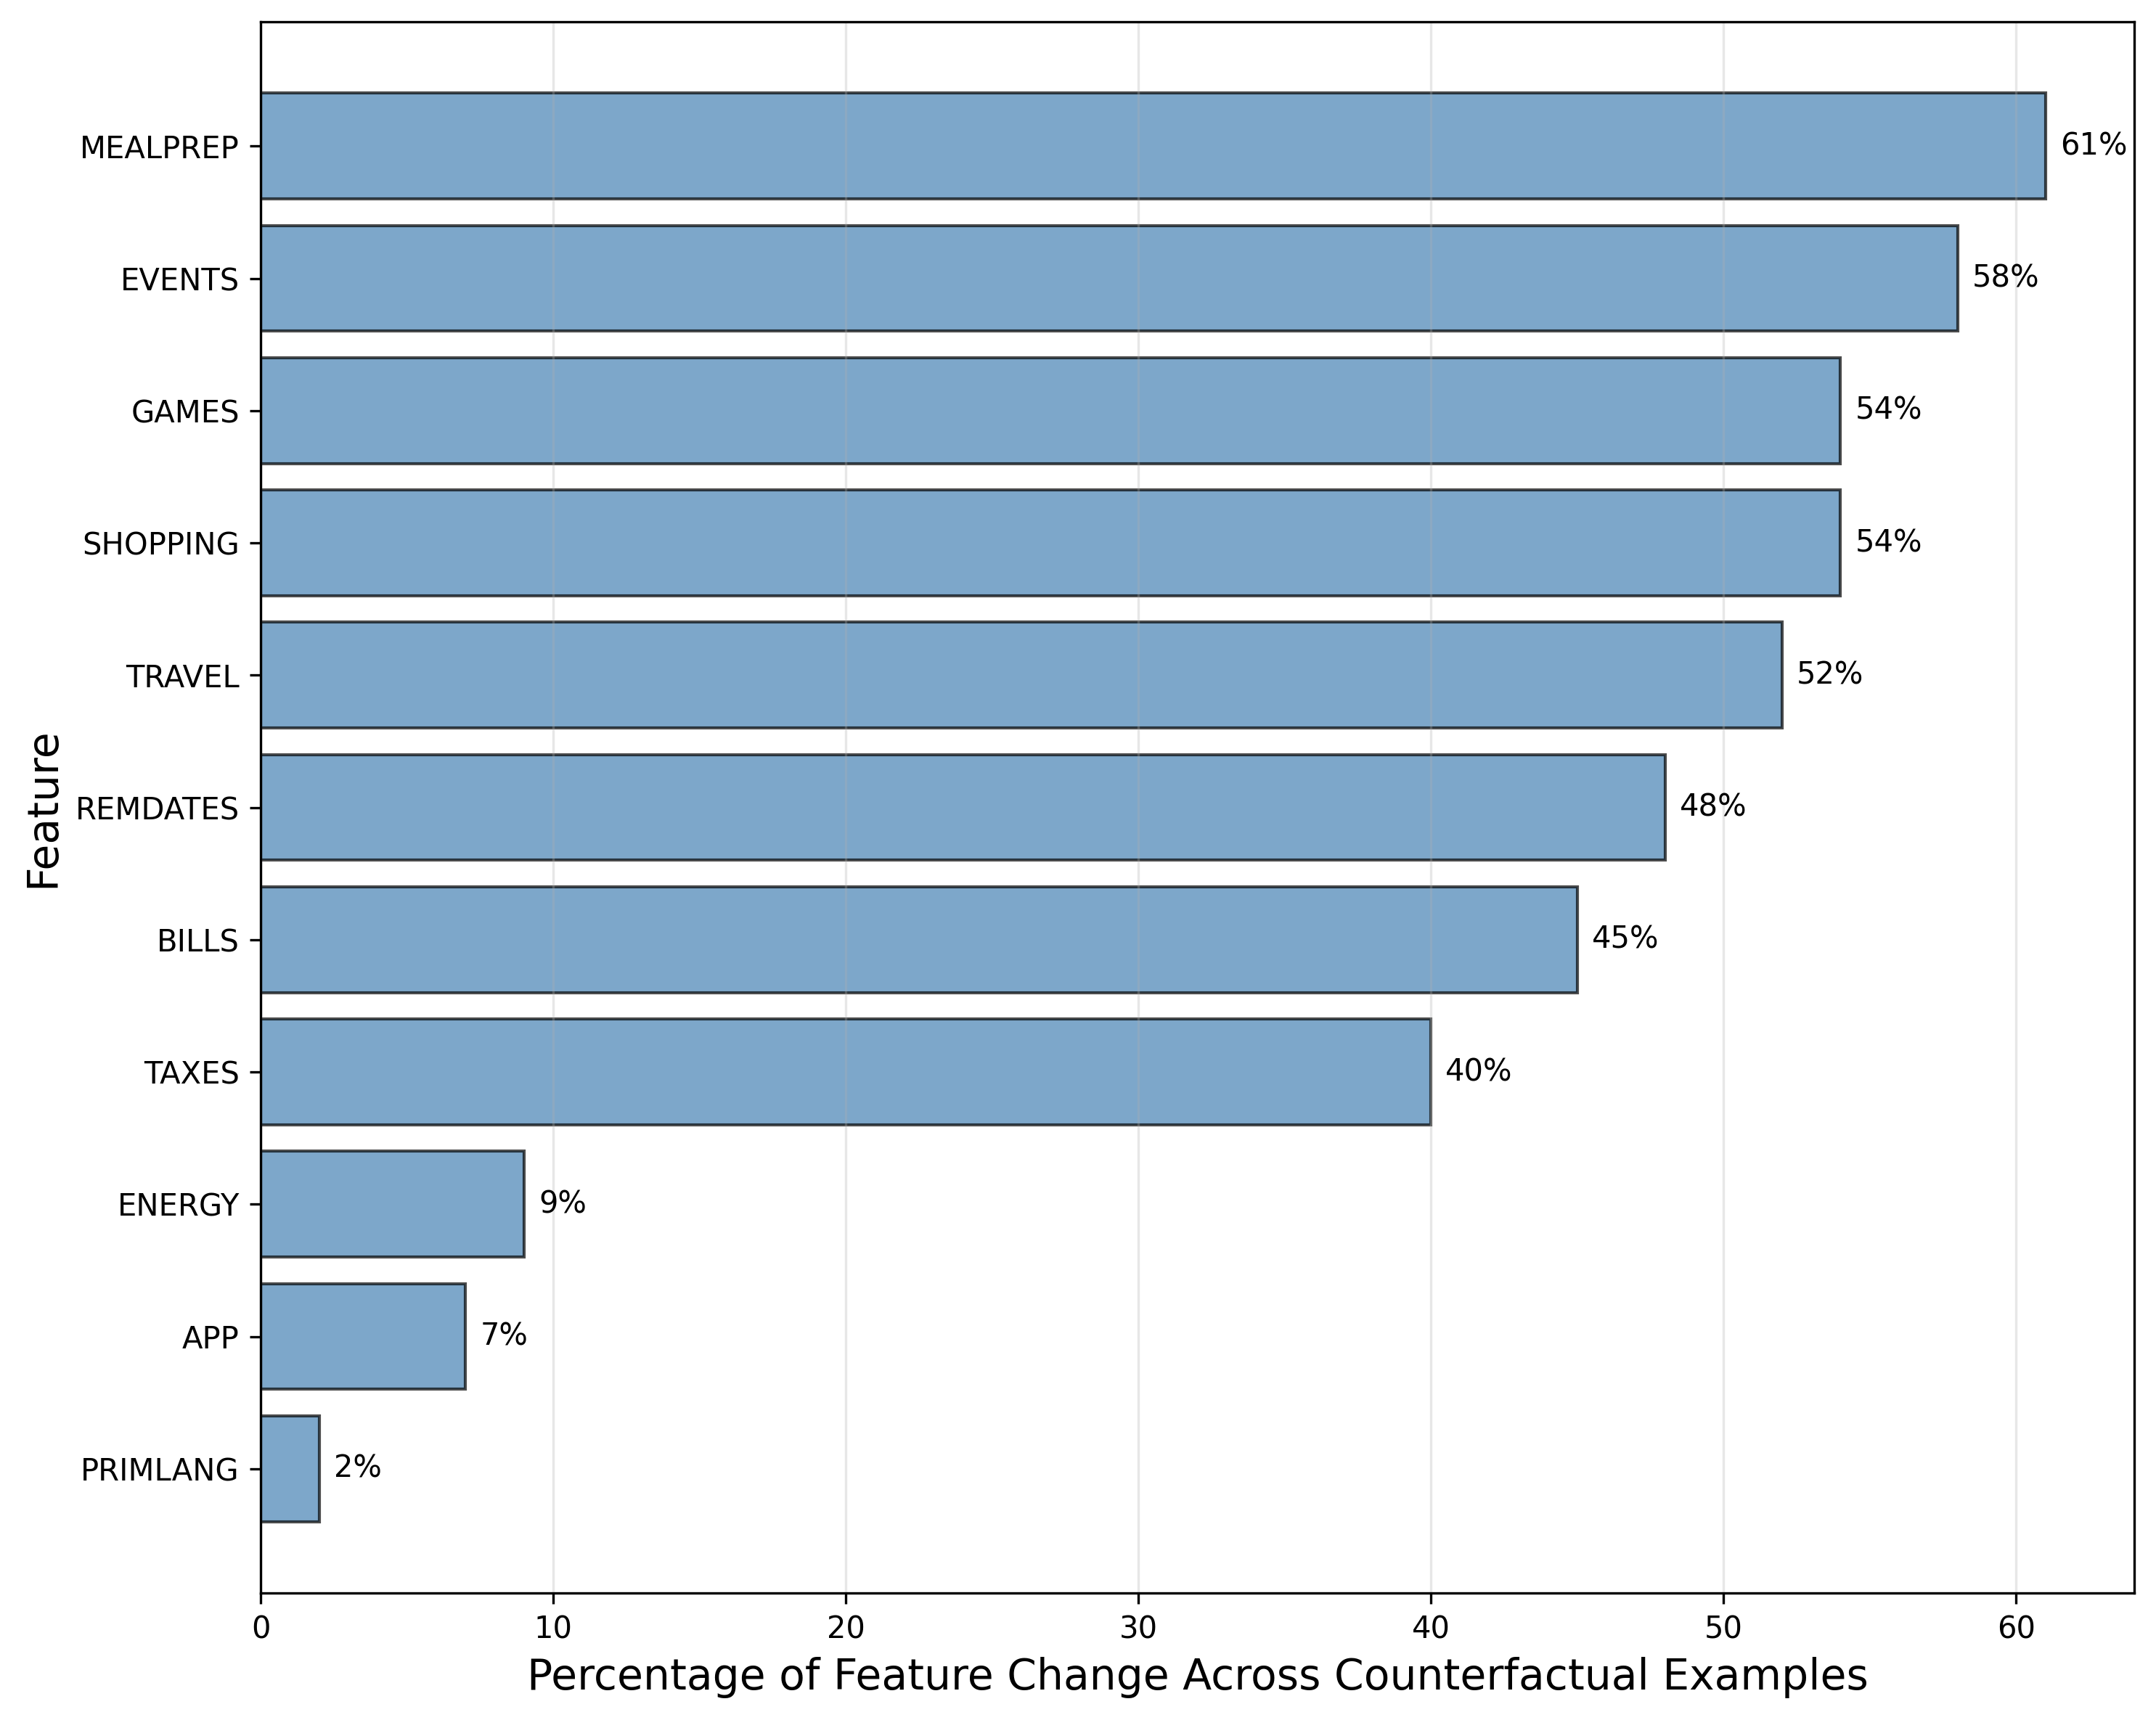
\includegraphics[width=1.0\textwidth]{figures/XAI/dementia_classification_adni_kdtree_dice_global_importance.png}
    \caption{Feature importance ranking based on counterfactual explanations for the CIND vs. dementia classification task}
    \begin{minipage}{\textwidth}
      \footnotesize The features are ranked based on the percentage of times they were modified to generate valid counterfactual examples. The rank highlights the most critical features for risk intervention.
    \end{minipage}
    \label{figure:cind_dementia_dice_feature_importance}
\end{figure}

\section{Future Cognitive Status Prediction Results}
This section presents the results for the second research objective, which focuses on developing cost-effective models to predict future cognitive status five years in advance. The same methodological steps were followed for feature selection, data resampling, model tuning and selection, and external validation. The section provides results for the normal cognition (NC) vs. cognitive impairment (CI) prediction task and the cognitive impairment but not dementia (CIND) vs. dementia prediction task.

\subsection{Feature Selection Results}
The results of the feature selection for the two cognitive status prediction tasks are presented in this subsection. The proposed feature selection method was evaluated against the baseline and the Boruta method by analyzing the performance and efficiency of the RF model and the degree of class overlap obtained from each method.

\subsubsection{Feature Selection Results for the Future NC vs. CI Prediction Task}

The feature selection evaluation was first conducted for the NC vs. CI prediction task. The comparison results for this prediction task are summarized in Table~\ref{table:fs-task3}. The RF model trained on all 66 baseline features achieved the highest G-mean (0.775), but also had the highest F1 class overlap score (0.961) and the lowest fitness score (0.646).

\begin{table}[!ht]
    \centering
    \caption{Comparison of feature selection methods for the future NC vs. CI prediction task}
    \begin{tabular}{|c|c|c|c|c|}
    \hline
        Method & Number of Features & G-mean & Fitness Score & F1 \\ \hline
        Baseline & 66 & 0.775 & 0.646 & 0.961 \\ \hline
        Boruta & 14 & 0.765 & 0.769 & 0.875 \\ \hline
        \textbf{Proposed Method} & \textbf{9} & \textbf{0.749} & \textbf{0.768} & \textbf{0.844} \\ \hline
        \multicolumn{5}{p{400pt}}{\footnotesize \hl{F1: Fisher's discriminant ratio (feature overlap measure), Fitness Score: combined score balancing performance and feature reduction, G-mean: geometric mean score.}}
    \end{tabular}
    \label{table:fs-task3}
\end{table}

The proposed method selected a minimal subset of only nine features. This was a more significant reduction than that of the Boruta method, which selected 14 features. As a result, the fitness score of the proposed method (0.768) was the highest among other methods. However, the nine selected features resulted in the lowest G-mean (0.749), which is 1.6 and 2.6 percentage points lower than the Boruta method and the baseline, respectively. This drop in RF model performance is compensated by the reduction in F1 class overlap score (0.844) and the increase in model training efficiency, which is approximately three times faster than the baseline.

Since the features selected by the proposed method resulted in the lowest RF performance, the features selected by the three methods were also tested using logistic regression LR and SVM. This is to analyze how the selected features perform across different models. The G-mean results of this analysis are presented in Table~\ref{table:fs-task3-more-models}. It can be observed that the baseline performance is the highest across all three models. However, a key finding is that the G-mean scores of the features selected by the proposed method are higher in the LR and SVM models compared to the RF model. The performance of these two models (LR and SVM) was comparable to the performance of the corresponding models trained on the 14 features selected by the Boruta method.

\begin{table}[!ht]
    \centering
    \caption{Comparison of feature selection methods in the future NC vs. CI prediction task based on G-mean performance across different models}
    \begin{tabular}{|c|c|c|c|c|}
    \hline
        Method & RF (G-mean) & LR (G-mean) & SVM (G-mean) \\ \hline
        Baseline (66 features) & 0.775 & 0.772 & 0.766 \\ \hline
        Boruta (14 features) & 0.765 & 0.759 & 0.763 \\ \hline
        Proposed Method (9 features) & 0.749 & 0.759 & 0.763 \\ \hline
        \multicolumn{4}{p{400pt}}{\footnotesize \hl{G-mean: geometric mean score, LR: logistic regression, RF: random forest, SVM: support vector machines.}}
    \end{tabular}
    \label{table:fs-task3-more-models}
\end{table}

From this supplementary analysis, it is clear that the proposed method is successful in finding the most minimal set of features that can reduce the complexity of the data and also improve the computational speed of the model. More importantly, the selected features generalize well when used with different classification algorithms.

The nine features that were selected by the proposed method for the NC vs. CI prediction task are listed in Table~\ref{table:features-task3}. The feature subset is composed of four categories of accessible data. Similarly to the previous classification tasks, this list is also heavily composed of IADL assessments from the FAQ, which account for 5 of the 9 features. The remaining items include demographic, memory complaint, and neuropsychiatric features. 

\begin{table}[h!]
\centering
\caption{List of selected features for the future NC vs. CI prediction task}
\label{table:features-task3}
\begin{tabular}{ccc}
\toprule
\textbf{Feature Code} & \textbf{Feature Description} & \textbf{Feature Category} \\
\midrule
NACCAGE & Age & Demographics \\
SEX & Sex & Demographics \\
MEMPROB & Subject reported memory problem & GDS \\
BILLS & Pay bills and track spending & FAQ \\
TAXES & Assemble tax records & FAQ \\
SHOPPING & Shop alone for necessities & FAQ \\
REMDATES & Remember dates and appointments & FAQ \\
TRAVEL & Travel out of neighborhood & FAQ \\
IRR & Irritability or lability in the last month & NPI-Q \\
\bottomrule
\end{tabular}
\end{table}

A comparison with the 12-feature set selected for the NC vs. CI classification task (Table~\ref{table:features-task1}) shows common selected features. Eight features are identical between both tasks, including NACCAGE, SEX, MEMPROB, and all five selected FAQ items. It should be noted that for this 5-year prediction task, the method did not select GAMES, EVENTS, and PAYATTN. It also selected IRR (irritability or lability) from the NPI-Q instead of ANX (anxiety). This results in a smaller, more focused set of features for the more difficult task of predicting future cognitive status.

\subsubsection{Feature Selection Results for the Future CIND vs. Dementia Prediction Task}
This subsection provides the results of the feature selection for the future CIND vs. dementia prediction task. Compared to the other classification and prediction tasks, this task is more challenging because it distinguishes the severity of cognitive impairment at five years in the future. The comparative results for this task are provided in Table~\ref{table:fs-task4}.

\begin{table}[!ht]
    \centering
    \caption{Comparison of feature selection methods for the future CIND vs. dementia prediction task}
    \begin{tabular}{|c|c|c|c|c|}
    \hline
        Method & Number of Features & G-mean & Fitness Score & F1 \\ \hline
        Baseline & 67 & 0.755 & 0.629 & 0.969 \\ \hline
        Boruta & 14 & 0.738 & 0.747 & 0.869 \\ \hline
        \textbf{Proposed Method} & \textbf{10} & \textbf{0.711} & \textbf{0.734} & \textbf{0.848} \\ \hline
        \multicolumn{5}{p{400pt}}{\footnotesize \hl{F1: Fisher's discriminant ratio (feature overlap measure), Fitness Score: combined score balancing performance and feature reduction, G-mean: geometric mean score.}}
    \end{tabular}
    \label{table:fs-task4}
\end{table}

The results show a pattern similar to that observed in the NC vs. CI prediction task. The baseline model achieved the highest G-mean (0.755), but had the lowest fitness score (0.629) and the highest F1 class overlap score (0.969). The proposed method identified a subset of ten features out of 67 features. This was smaller than the 14 features selected by the Boruta method. This set of 10-features also achieved the lowest F1 class overlap score (0.848), indicating that it was the most effective method to reduce the high complexity of this task.

In this prediction task, the features selected by the Boruta method resulted in a higher G-mean (0.738) than the proposed method's (0.711). Therefore, the Boruta method achieved the highest fitness score (0.747) in this task. However, the proposed method selected the smallest set of features and was the most cost-effective in terms of computation, with a training speed 2.9 times faster than the baseline. Additionally, its fitness score of 0.734 was significantly better than the baseline. This shows that the proposed feature selection method is able to find a strong balance between simplicity and performance even in the most difficult prediction task.

To further support this claim, the performance of the selected features of the three methods was evaluated using two more classifiers (LR and SVM) in addition to RF. The comparison of the G-mean of the three models is presented in Table~\ref{table:fs-task4-more-models}. The results are similar to those of the NC vs. CI prediction task, which can be seen in Table~\ref{table:fs-task3-more-models}. The analysis revealed that the baseline continually performs the best in all three models. However, it can be observed that the performance of the LR and SVM models trained on the ten features selected by the proposed method shows a significant increase compared to the RF performance. The G-mean scores of these two models were slightly higher than the corresponding LR and SVM models based on the Boruta method. This finding demonstrates that the proposed method can select a set of features that can produce comparable performance across different models.

\begin{table}[!ht]
    \centering
    \caption{Comparison of feature selection methods in the future CIND vs. dementia prediction task based on G-mean performance across different models}
    \begin{tabular}{|c|c|c|c|c|}
    \hline
        Method & RF (G-mean) & LR (G-mean) & SVM (G-mean) \\ \hline
        Baseline (67 features) & 0.755 & 0.765 & 0.771 \\ \hline
        Boruta (14 features) & 0.738 & 0.76 & 0.756 \\ \hline
        Proposed Method (10 features) & 0.711 & 0.761 & 0.758 \\ \hline
        \multicolumn{4}{p{400pt}}{\footnotesize \hl{G-mean: geometric mean score, LR: logistic regression, RF: random forest, SVM: support vector machines.}}
    \end{tabular}
    \label{table:fs-task4-more-models}
\end{table}

The subset of features selected by the proposed method is provided in Table~\ref{table:features-task4}. Similar to the other tasks, the list is dominated by the IADL assessments from the FAQ, which contribute 7 of the 10 features. The remaining features are the body mass index and two GDS items that survey problems with memory and energy level. More details of the selected features and their correlation results can be found in section \ref{sec:feature-selection-apdx} in the appendix.

\begin{table}[h!]
\centering
\caption{List of selected features for the future CNID vs. dementia prediction task}
\label{table:features-task4}
\begin{tabular}{ccc}
\toprule
\textbf{Feature Code} & \textbf{Feature Description} & \textbf{Feature Category} \\
\midrule
NACCBMI & Body Mass Index (\acrshort{BMI}) & Physical Assessment \\
MEMPROB & Subject reported memory problem & GDS \\
ENERGY & Do you feel full of energy? & GDS \\
BILLS & Pay bills and track spending & FAQ \\
TAXES & Assemble tax records & FAQ \\
SHOPPING & Shop alone for necessities & FAQ \\
MEALPREP & Prepare a balanced meal & FAQ \\
EVENTS & Keep track of current events & FAQ \\
REMDATES & Remember dates and appointments & FAQ \\
TRAVEL & Travel out of neighborhood & FAQ \\
\bottomrule
\end{tabular}
\end{table}


\subsection{Data Resampling Results}

\label{sec:resampling_results_ro2}
This section details the data resampling results related to the second research objective, which focuses on the 5-year future prediction of cognitive impairment. As reflected in the training datasets, the prediction of the future cognitive status is an inherently more complex problem. Therefore, applying the systematic data resampling was necessary to address the significant class imbalance and overlap challenges and to develop accurate and well-balanced prediction models. The distribution of the target classes in the NACC UDS and ADNI datasets is provided in Figure~\ref{fig:nacc-data-stat} and Figure~\ref{fig:adni-data-stat} in the appendix.

\subsubsection{Data Resampling Results for the Future NC vs. CI Prediction Task}
\label{sec:resampling_future_nc_ci}
The training dataset for the future NC vs. CI prediction task was first examined. It presented a slight class imbalance with an IR of 1.18, where the CI class was the minority. However, a high degree of data complexity was noticeable. The instance-level class overlap (kDN) score was 0.274, and the structural class overlap (N1) was particularly high at 0.389. The analysis of borderline instances showed that 26\% of the minority class (CI) and 31\% of the majority class (NC) resided in these overlapped regions.

To handle this high data complexity, the ENN + \acrshort{BorderlineSMOTE} strategy was selected by the decision algorithm (Algorithm \ref{alg:data-resampling}). The ENN method was first utilized to remove noisy instances. Since the minority class is less represented on the decision boundary, BorderlineSMOTE is used to carefully add synthetic minority class examples in this critical region. The impact of this strategy on the RF model was compared with the baseline and other data resampling methods. The comparison results are presented in Table~\ref{table:future_nc_ci_resampling}. Figure~\ref{figure:future_nc_ci_resampling_perf} provides a visual presentation of the results.

\begin{table}[!ht]
    \centering
    \caption{Performance comparison of resampling methods for the future NC vs. CI prediction task using a random forest model}
    \begin{tabular}{|c|c|c|c|c|c|}
    \hline
        Method & G-mean & Recall (NC) & Recall (CI) & kDN & N1 \\ \hline
        Baseline & 0.749 & \textbf{0.870} & 0.644 & 0.274 & 0.389 \\ \hline
        ROS & \makecell{0.749 \\ {\small \hl{(p = 0.972)}}} & 0.853 & 0.658 & 0.272 & 0.385 \\ \hline
        RUS & \makecell{0.752 \\ {\small \hl{(p = 0.175)}}} & 0.845 & 0.669 & 0.229 & 0.365 \\ \hline
        SMOTE & \makecell{0.751 \\ {\small \hl{(p = 0.135)}}} & 0.860 & 0.656 & 0.267 & 0.446 \\ \hline
        \makecell{\textbf{ENN +} \\ \textbf{BorderlineSMOTE}} & \makecell{\textbf{0.752} \\ {\small \hl{(p = 0.343)}}} & 0.812 & \textbf{0.697} & \textbf{0.018} & \textbf{0.158} \\ \hline
        \multicolumn{6}{p{400pt}}{\footnotesize \hl{G-mean: geometric mean score, kDN: k-disagreeing neighbors (instance-level class overlap), N1: structural class overlap, Recall: per-class recall.}}
    \end{tabular}
    \label{table:future_nc_ci_resampling}
\end{table}

\begin{figure}[ht]
\centering
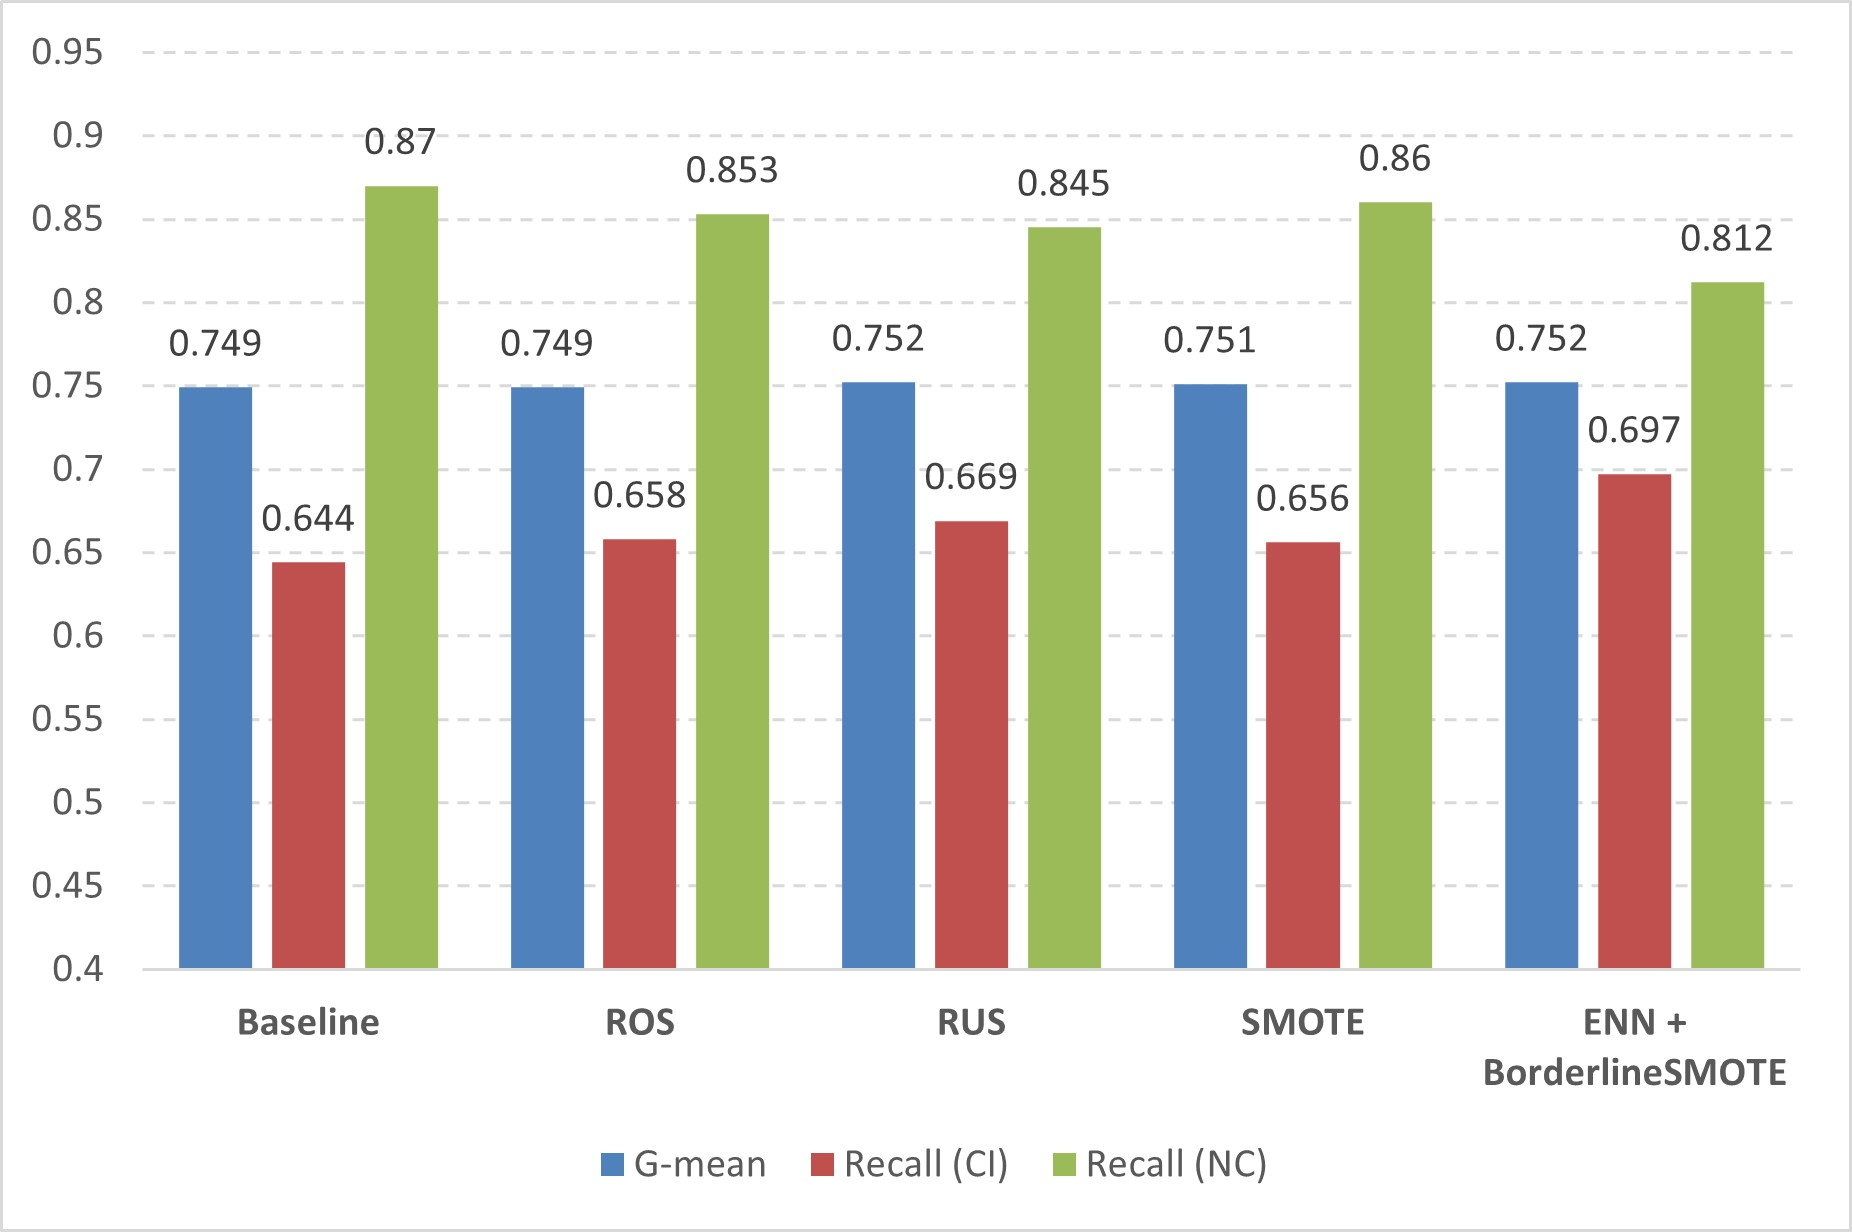
\includegraphics[width=1\textwidth]{figures/data-resampling-task3.jpg}
\caption{Model performance comparison of data resampling methods for the future NC vs. CI prediction task}
\label{figure:future_nc_ci_resampling_perf}
\end{figure}

The baseline performance, as shown in Table~\ref{table:future_nc_ci_resampling}, was heavily affected by the data complexity. The model struggled to identify the minority CI class, resulting in a low recall of 0.644. Standard methods like ROS and SMOTE did not result in any significant improvement. A key observation is that SMOTE worsened structural class overlap (N1 increased to 0.446) and provided no noticeable improvement to G-mean or recall.

The selected ENN + BorderlineSMOTE method achieved the highest balanced performance with a G-mean of 0.752. The reduction in class overlap might have allowed the RF model to learn a better decision boundary, which is reflected in the significant increase in the minority CI class recall from 0.644 to 0.697, while the NC class recall decreased from 0.870 to 0.812. \hl{The G-mean improvement of the proposed ENN + BorderlineSMOTE method over the baseline was not statistically significant (p = 0.343). This is expected, since the main benefit of the method is the reduction of class overlap rather than a direct gain in G-mean, which confirms that the synthetic data did not artificially inflate the performance.}

\subsubsection{Data Resampling Results for the Future CIND vs. Dementia Prediction Task}
\label{sec:resampling_future_cind_dem}
A similar analysis was performed for the future CIND vs. dementia prediction task. The training dataset of this task showed an IR of 1.46, with CIND as the minority class. This task presented a very high data complexity, with a kDN of 0.260 and a very high structural class overlap (N1) of 0.485. The minority class (CIND) has 39\% of its instances at the borderline compared to 26\% of the majority class (dementia) instances.

Based on this high complexity, the ENN + KMeansSMOTE method was selected by the decision algorithm (Algorithm \ref{alg:data-resampling}). This strategy was chosen to clean the noisy decision boundary with ENN, while KMeansSMOTE was applied to reinforce the sparse clusters of the minority CIND class. The performance of this method was compared with other standard techniques in Table~\ref{table:future_cind_dem_resampling}. The comparison results are also demonstrated in Figure~\ref{figure:future_cind_dem_resampling_perf}.

\begin{table}[!ht]
    \centering
    \caption{Performance comparison of resampling methods for the future CIND vs. dementia prediction task using a random forest model}
    \begin{tabular}{|c|c|c|c|c|c|}
    \hline
        Method & G-mean & Recall (Dementia) & Recall (CIND) & kDN & N1 \\ \hline
        Baseline & 0.711 & 0.770 & 0.656 & 0.260 & 0.485 \\ \hline
        ROS & \makecell{0.715 \\ {\small \hl{(p = 0.101)}}} & 0.754 & 0.678 & 0.244 & 0.469 \\ \hline
        RUS & \makecell{0.726 \\ {\small \hl{(p = 0.014)}}} & 0.723 & \textbf{0.728} & 0.250 & 0.470 \\ \hline
        SMOTE & \makecell{0.715 \\ {\small \hl{(p = 0.314)}}} & 0.758 & 0.675 & 0.238 & 0.432 \\ \hline
        \makecell{\textbf{ENN +} \\ \textbf{KMeansSMOTE}} & \makecell{\textbf{0.730} \\ {\small \hl{(p = 0.022)}}} & \textbf{0.776} & 0.688 & \textbf{0.034} & \textbf{0.161} \\ \hline
        \multicolumn{6}{p{400pt}}{\footnotesize \hl{G-mean: geometric mean score, kDN: k-disagreeing neighbors (instance-level class overlap), N1: structural class overlap, Recall: per-class recall.}}
    \end{tabular}
    \label{table:future_cind_dem_resampling}
\end{table}

\begin{figure}[H]
\centering
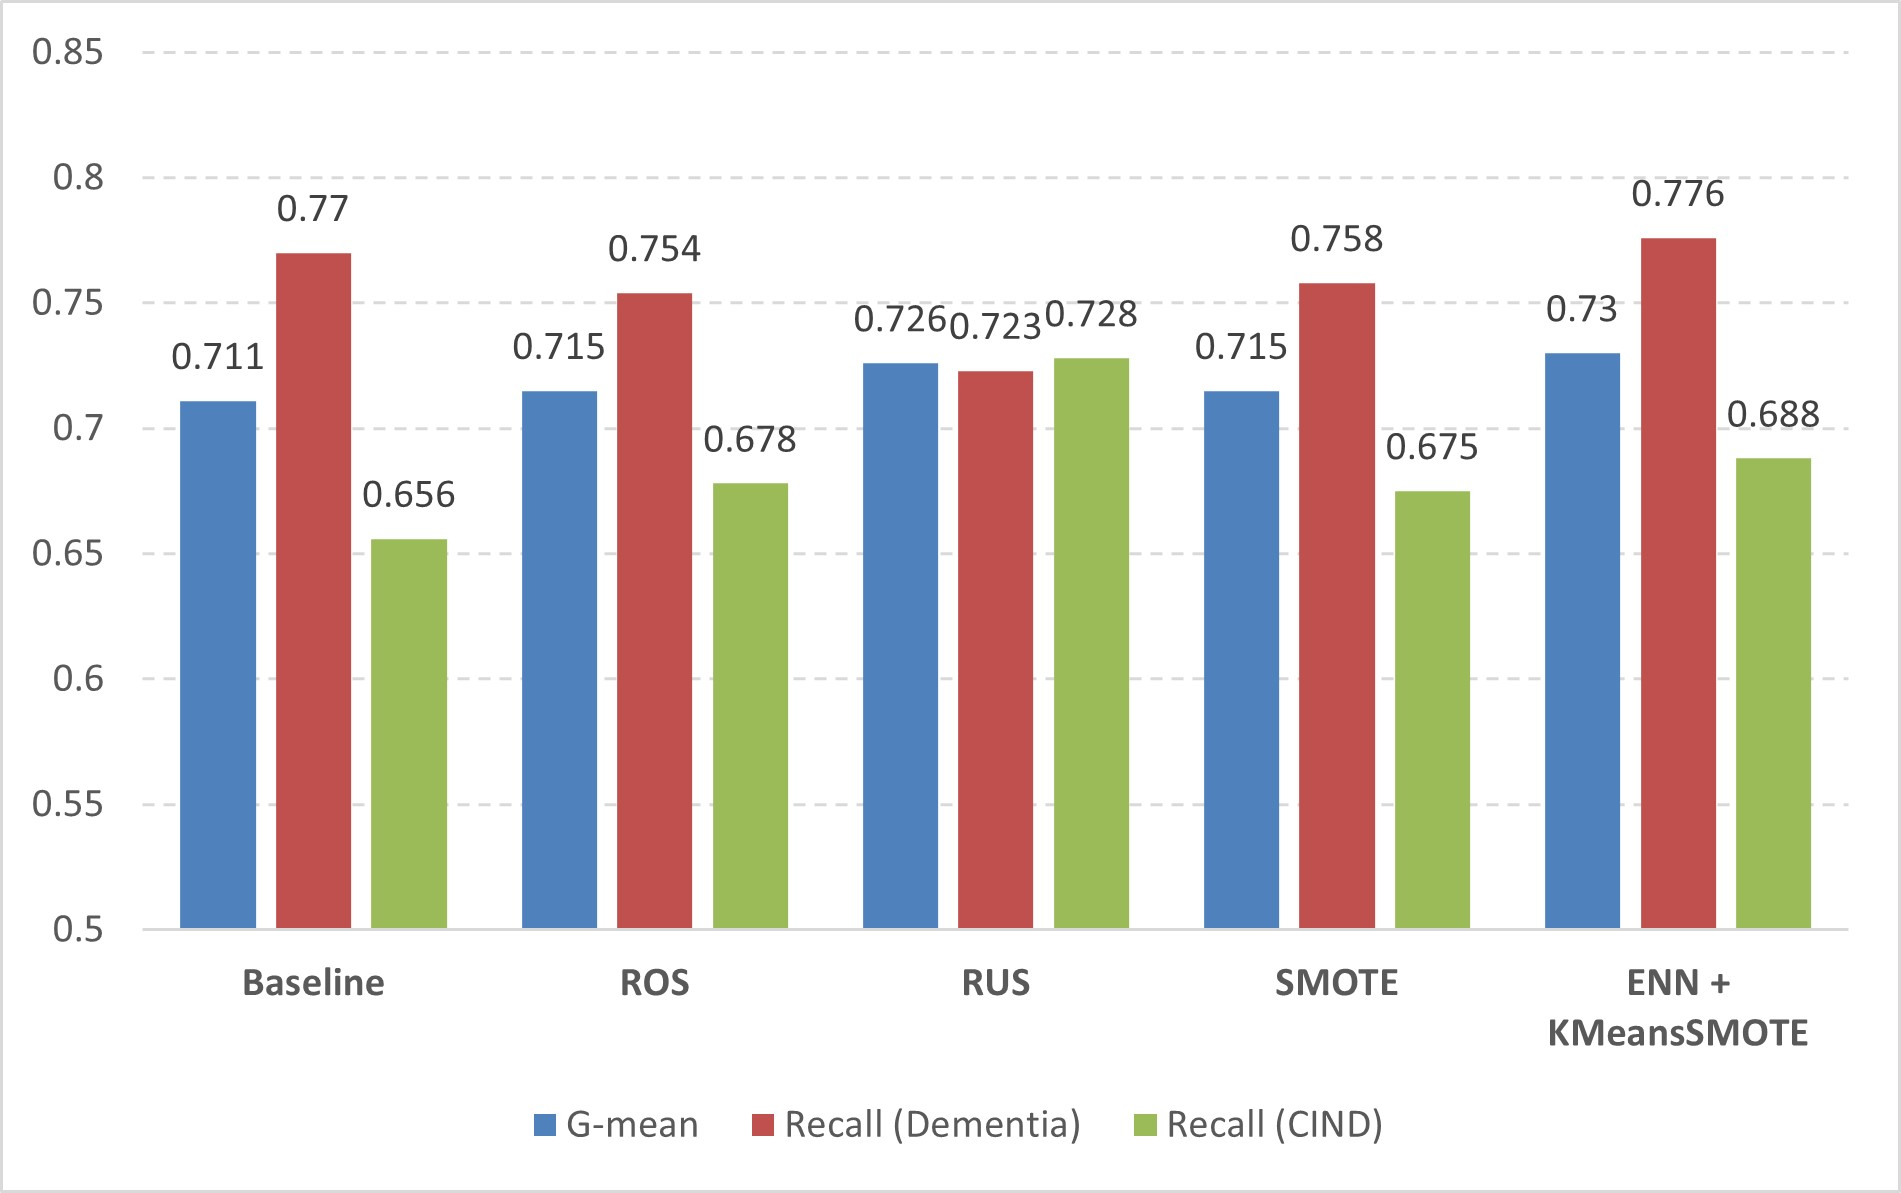
\includegraphics[width=1\textwidth]{figures/data-resampling-task4.jpg}
\caption{Model performance comparison of data resampling methods for the future CIND vs. dementia prediction task}
\label{figure:future_cind_dem_resampling_perf}
\end{figure}

The baseline model experienced classification complexity due to the high class overlap in this task. As a result, the model had a low G-mean of 0.711 and a poor recall for the minority CIND class (0.656). The RUS method reduced the density of the majority class, which slightly lowered the class overlap. This allowed the RF model to achieve the highest recall of the minority CIND class (0.728) and to improve the baseline G-mean to 0.726. However, it removed informative patterns of the dementia class, resulting in the most significant drop in dementia recall from 0.770 to 0.723. This outcome might not be acceptable, as misclassifying dementia cases could have a higher risk and cost. A similar outcome was observed in the ROS and SMOTE methods, with both methods slightly improving the baseline G-mean to 0.715.

The ENN + KMeansSMOTE method increased the G-mean to 0.730. This method was the only one that improved the recall for both classes simultaneously. \hl{This G-mean improvement over the baseline was statistically significant (p = 0.022), which supports the reliability of the proposed overlap-aware strategy.} This high performance is explained by the significant reduction in data complexity. By cleaning the data, the method improved the model's recall on the difficult minority CIND class from 0.656 to 0.688 while also slightly improving the recall on the dementia class.

In conclusion, the baseline model suffered from high class overlap in both future prediction tasks. The overlap-guided resampling methodology produced highly effective results. It successfully identified and applied hybrid techniques that reduced the data complexity and improved the model's ability to classify both classes more accurately. These results move the outcomes of this study closer to achieving the research objectives and improve the training data quality for better modeling results, which are highlighted in the next subsections.

\subsection{Model Fine-tuning and Selection Results}
Following the feature selection and data resampling stages, the hyperparameters of five classification models were optimized, and the most cost-effective model was selected. This section details the results of this process for the two tasks to predict cognitive status up to five years in the future.

\subsubsection{Model Fine-tuning and Selection Results for the Future NC vs. CI Prediction Task}
The cost-effective model selection algorithm (Algorithm \ref{alg:model-selection}) was applied to the grid search results for the five prediction models. The primary objective was to find model hyperparameters that maintain high performance while increasing efficiency. The training throughput of the LightGBM model increased by 3.59 times, and the prediction throughput showed around a three-times increase. This was done with a minor decrease in performance compared to the best-performing LightGBM model (the F1-score was dropped from 0.751 to 0.744). Similarly, substantial improvement in prediction speed was shown by the KNN model. Table~\ref{table:task3_finalists_models} summarizes the performance and efficiency metrics of the five models selected by the algorithm.

\begin{table}[!ht]
\centering
\caption{Summary of fine-tuned models for the future NC vs. CI prediction task}
\label{table:task3_finalists_models}
\newcolumntype{C}{>{\centering\arraybackslash}X}
    \begin{tabularx}{\textwidth}{|C|C|C|C|C|}
        \hline
        \textbf{Model} &
        \textbf{F1-score (95\% CI)} &
        \textbf{G-mean (95\% CI)} &
        \textbf{Training Throughput (Gain)\textsuperscript{1}} &
        \textbf{Prediction Throughput (Gain)\textsuperscript{1}} \\
        \hline
        KNN &
        0.723 ($\pm 0.002$) &
        0.750 ($\pm 0.002$) &
        $1,044,635$ $(1.03\times)$ &
        $48,105$ $(2.64\times)$ \\
        \hline
        LR &
        0.747 ($\pm 0.002$) &
        0.770 ($\pm 0.002$) &
        $819,113$ $(1.04\times)$ &
        $6,630,848$ $(1.07\times)$ \\
        \hline
        LightGBM &
        0.744 ($\pm 0.003$) &
        0.756 ($\pm 0.003$) &
        $114,209$ $(3.59\times)$ &
        $710,044$ $(2.93\times)$ \\
        \hline
        RF &
        0.750 ($\pm 0.004$) &
        0.769 ($\pm 0.004$) &
        $27,856$ $(1.05\times)$ &
        $186,313$ $(1.06\times)$ \\
        \hline
        SVM &
        0.747 ($\pm 0.003$) &
        0.768 ($\pm 0.003$) &
        $2,647$ $(1.02\times)$ &
        $20,074$ $(1.28\times)$ \\
        \hline
        \multicolumn{5}{p{400pt}}{\footnotesize \textsuperscript{1}\hl{Training throughput is reported in training samples per second, and prediction throughput in predictions per second.} Gain is calculated as the ratio of the selected model’s throughput to the benchmark model’s throughput. Values indicate the factor by which training and prediction speed have improved.}
    \end{tabularx}
\end{table}

To select a single best model for this prediction task, a final assessment was performed. The assessment compares the models according to performance, efficiency, and interpretability. Based on the results in Table~\ref{table:task3_finalists_models}, the LR model was chosen as the final model.

The LR model outperformed other models in multiple criteria. In terms of performance, the LR model was one of the best-performing models, achieving an F1-score of 0.747. This score is similar to the performance achieved by the SVM and LightGBM models. The RF model obtained a marginally better F1-score of 0.750. The KNN model continued to achieve the lowest performance as observed in the other classification tasks. With multiple models scoring high performance, efficiency was assessed to differentiate them. Superior computational speed was exhibited by the LR model, with a prediction throughput of over 6.6 million samples per second. This is extremely faster than the RF, SVM, and LightGBM models. Finally, the interpretability of the model is crucial for this study. As a linear model, LR allows for a straightforward explanation of how risk factors influence the prediction of future cognitive impairment. A significant advantage is offered by this over the complex, non-linear nature of the RF and SVM models. Therefore, the overall balance of comparable accuracy, high speed, and easy interpretability justify the selection of the LR model. Table~\ref{table:lr-fine-tune-task3-apdx} in the appendix presents the hyperparameter fine-tuning results of the LR model.

\subsubsection{Model Fine-tuning and Selection Results for the Future CIND vs. Dementia Prediction}
Similar to the previous task, the cost-effective selection algorithm was utilized to filter the models generated by the grid search hyperparameters fine-tuning. The algorithm found highly efficient hyperparameters for the RF, LightGBM, and KNN models. A particularly substantial improvement was found for the RF model, where the selected model achieved around a three-times increase in training and prediction speed compared to the benchmark model (RF model with the highest performance). This was obtained with only a marginal reduction in performance. A similar increase in training and prediction speed was observed in the LightGBM model. The LR model also saw a lower degree of increase in training and prediction speed. Table~\ref{table:task4_finalists_models} details the performance metrics and throughput gains for the five selected models.

\begin{table}[!ht]
\centering
\caption{Summary of fine-tuned models for the future CIND vs. dementia Prediction Task}
\label{table:task4_finalists_models}
\newcolumntype{C}{>{\centering\arraybackslash}X}
    \begin{tabularx}{\textwidth}{|C|C|C|C|C|}
        \hline
        \textbf{Model} &
        \textbf{F1-score (95\% CI)} &
        \textbf{G-mean (95\% CI)} &
        \textbf{Training Throughput (Gain)\textsuperscript{1}} &
        \textbf{Prediction Throughput (Gain)\textsuperscript{1}} \\
        \hline
        KNN &
        0.772 ($\pm 0.014$) &
        0.732 ($\pm 0.014$) &
        $1,003,616$ $(1.14\times)$ &
        $61,623$ $(3.15\times)$ \\
        \hline
        LR &
        0.773 ($\pm 0.011$) &
        0.757 ($\pm 0.009$) &
        $744,495$ $(1.14\times)$ &
        $5,276,181$ $(1.41\times)$ \\
        \hline
        LightGBM &
        0.770 ($\pm 0.014$) &
        0.751 ($\pm 0.012$) &
        $58,983$ $(2.67\times)$ &
        $386,914$ $(2.46\times)$ \\
        \hline
        RF &
        0.780 ($\pm 0.016$) &
        0.751 ($\pm 0.015$) &
        $17,395$ $(3.15\times)$ &
        $130,213$ $(3.00\times)$ \\
        \hline
        SVM &
        0.772 ($\pm 0.011$) &
        0.756 ($\pm 0.013$) &
        $9,608$ $(1.07\times)$ &
        $46,531$ $(1.09\times)$ \\
        \hline
        \multicolumn{5}{p{400pt}}{\footnotesize \textsuperscript{1}\hl{Training throughput is reported in training samples per second, and prediction throughput in predictions per second.} Gain is calculated as the ratio of the selected model’s throughput to the benchmark model’s throughput. Values indicate the factor by which training and prediction speed have improved.}
    \end{tabularx}
\end{table}

The LR model was subsequently selected as the most cost-effective model. This decision is explained by a balanced evaluation of three criteria. First, the LR model obtained an F1-score of 0.773. Slightly higher scores of 0.780 and 0.777 were achieved by the RF model and the LightGBM model, respectively. Second, in terms of efficiency, the LR model offers a prediction throughput of over 5.2 million samples per second, which is much faster than all other models. Finally, the transparency of the linear LR model allows a clear interpretation of predictive factors. The RF and LightGBM models are less interpretable and significantly more computationally expensive. Therefore, the LR model was again selected as the final model for this classification task because it provides a considerable balance between performance and computational efficiency, as well as easy interpretation of the prediction. The hyperparameter fine-tuning results of the LR model is presented in Table~\ref{table:lr-fine-tune-task4-apdx} in the appendix.

In summary, the application of the fine-tuning and selection methodology to the future cognitive status prediction tasks has produced similar results to the current classification tasks. For both the NC vs. CI and CIND vs. dementia prediction tasks, the LR model was identified as the most suitable candidate. These findings confirm the feasibility of using cost-effective and explainable models for predicting future cognitive decline. The following section will evaluate the generalizability of these selected models using external validation data.

\subsection{Model Performance in External Validation}
The two selected LR models for the prediction of cognitive status 5 years in the future were tested using two separate datasets to assess their generalizability. First, the models were tested on the holdout NACC cross-center testing dataset (which represents 20\% of the original data) to evaluate their performance on unseen data from different research centers. In addition, an independent external validation was performed using the ADNI dataset. Moreover, the results of the models' calibration and clinical utility evaluation in both external validation datasets were presented. The details of the validation method are described in section \ref{sec:model-validation}.

\subsubsection{External Validation Results for the Future NC vs. CI Prediction Task}
The performance of the LR model to predict the future risk of CI was analyzed across the internal and external validation datasets. A comparison of performance metrics is provided in Table~\ref{tab:future_nc_ci_results}. Additionally, the ROC curves for the three validation stages are shown in Figure~\ref{fig:future_nc_ci_roc}.

\begin{table}[!ht]
    \centering
    \caption{Performance of the selected logistic regression model in internal and external validation for the future NC vs. CI prediction task}
    \label{tab:future_nc_ci_results}
    \newcolumntype{C}{>{\centering\arraybackslash}X}
        \begin{tabularx}{\textwidth}{|c|c|C|C|}
            \hline
            \textbf{Metric} & \textbf{Internal CV} & \textbf{NACC Cross-center Validation} & \textbf{ADNI External Validation} \\
            \hline
            AUC & \makecell{0.772 \\ {\small \hl{(0.769--0.776)}}} & \makecell{0.790 \\ {\small \hl{(0.774--0.806)}}} & \makecell{0.778 \\ {\small \hl{(0.750--0.803)}}} \\ \hline
            G-mean & 0.770 & 0.787 & 0.777 \\ \hline
            Sensitivity & 0.723 & 0.721 & 0.745 \\ \hline
            Specificity & 0.820 & 0.859 & 0.810 \\ \hline
            F1-score & 0.747 & 0.772 & 0.791 \\
            \hline
             \multicolumn{4}{p{400pt}}{\footnotesize \hl{AUC: area under the curve, F1-score: harmonic mean of precision and recall, G-mean: geometric mean score, Sensitivity: recall of the CI class, Specificity: recall of the NC class.}}
        \end{tabularx}
\end{table}

\begin{figure}[ht]
    \centering
    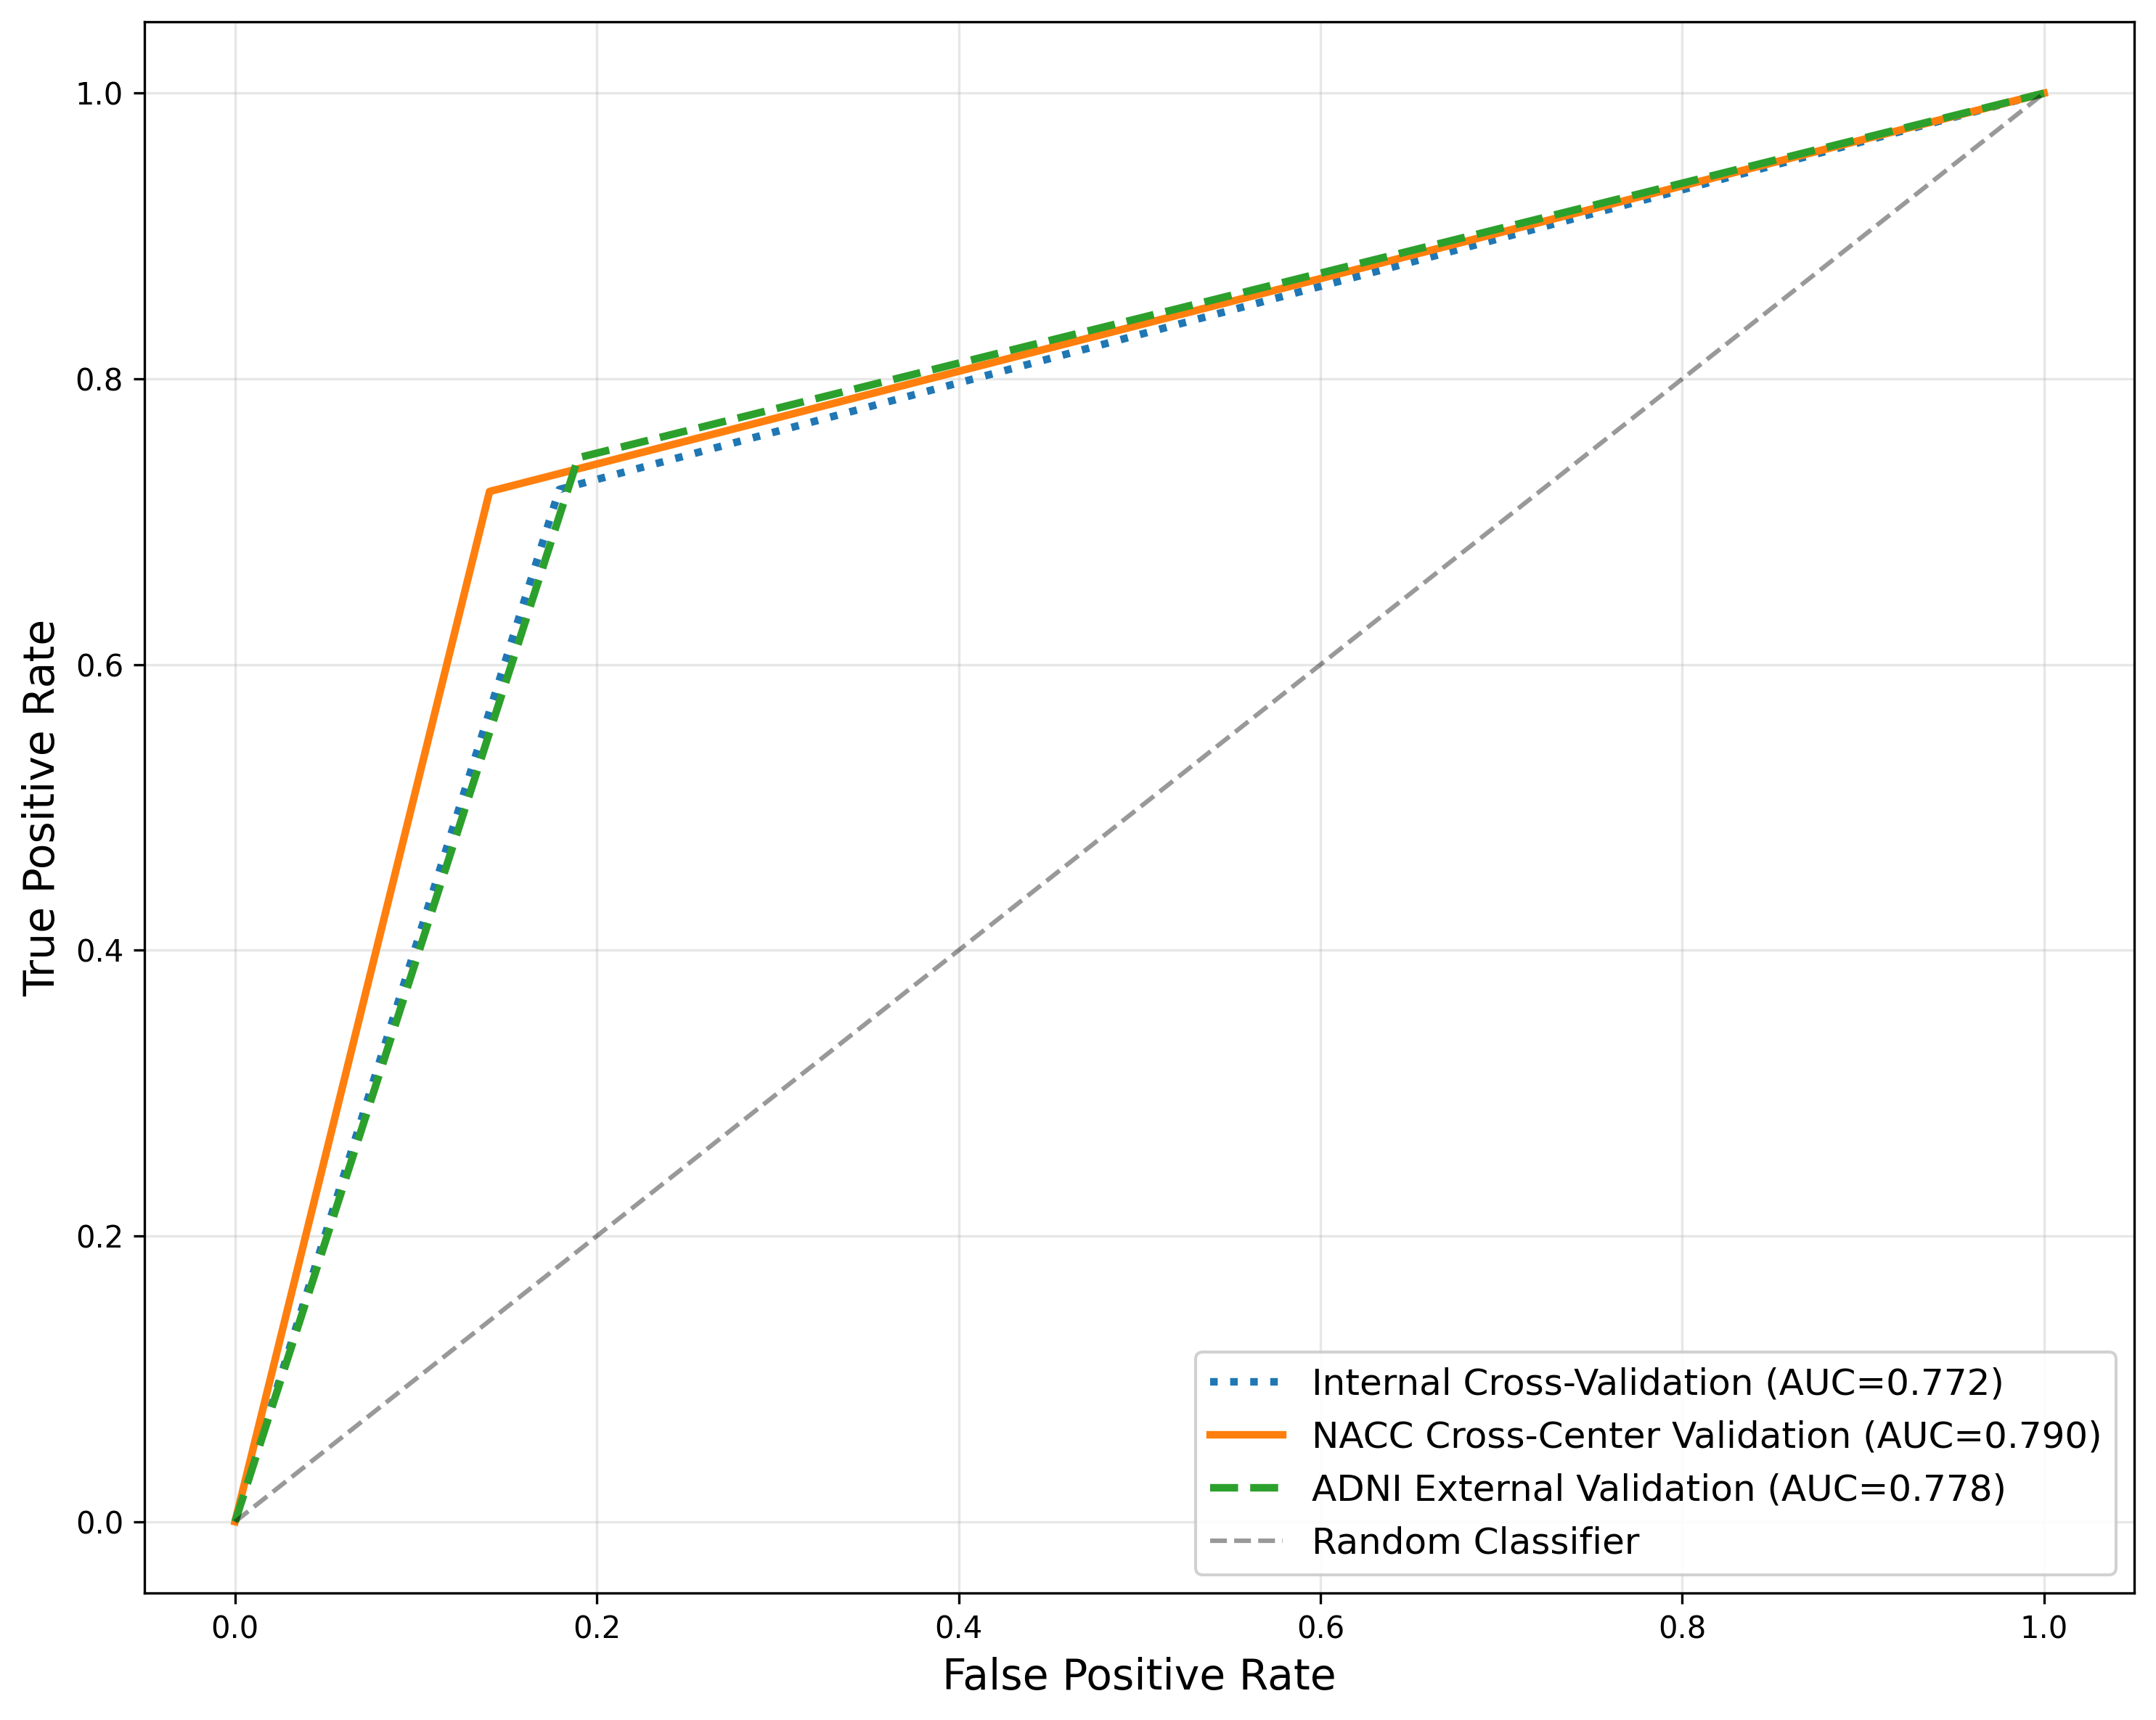
\includegraphics[width=0.7\textwidth]{figures/impaired_prediction_all_tests_roc_overlay.png}
    \caption{ROC curves comparing the performance of the logistic regression model for the future NC vs. CI prediction task}
    \begin{minipage}{\textwidth}
      \footnotesize \hl{The horizontal axis shows the false positive rate (1 -- specificity) and the vertical axis shows the true positive rate (sensitivity). Each curve represents one validation dataset.}
    \end{minipage}
    \label{fig:future_nc_ci_roc}
\end{figure}

The results of the NACC cross-center validation showed an improvement in performance compared to the internal CV. Unlike the results of the current cognitive status classification task (section \ref{sec:classification_external_validation}), the AUC score increased from 0.772 to 0.790, and the G-mean improved from 0.770 to 0.787. This improvement is attributed to the significant increase in NC recall (specificity) from 0.820 to 0.859, while the CI recall had a very minimal decrease. These findings suggest that the model was exceptionally well generalized to the unseen NACC data collected in different research centers.

The model also demonstrated high performance when applied to the ADNI dataset. The AUC score of 0.778 is very close to the internal CV score and only slightly lower than the NACC cross-center validation score. This can be observed in Figure~\ref{fig:future_nc_ci_roc} as the ADNI external validation's ROC curve is close to the other curves. Importantly, the sensitivity was 0.745 in the ADNI external validation, which outperformed the sensitivity of the other two validations. This indicates that the model is reliable in identifying cases at risk of future CI in a different clinical population. However, the model scored the lowest NC recall of 0.810 in the ADNI external validation. \hl{Both external AUC scores differed significantly from the internal CV (NACC cross-center p < 0.001, ADNI p = 0.036), although the differences were small and within an acceptable range for generalization.} Table~\ref{table:lr-complete-perf-task3-apdx} in the appendix provides extended performance metrics of the external validation results.

Calibration of the LR model was also performed to produce a reliable estimate of future CI risk. Figure~\ref{fig:future_nc_ci_calib_curve} demonstrates the calibration curves for both validation datasets. In the NACC cross-center validation, the uncalibrated model overestimated the risk at most of the interval and generated extreme probabilities close to 0 and 1. After beta calibration was applied, the distribution of the predicted probabilities was corrected with excellent intercept and slope. As a result, the ECE was significantly reduced from 0.108 to 0.023, and the Brier score improved from 0.164 to 0.148. This indicates excellent calibration and accuracy of the model's prediction.

\begin{figure}[ht]
    \centering
    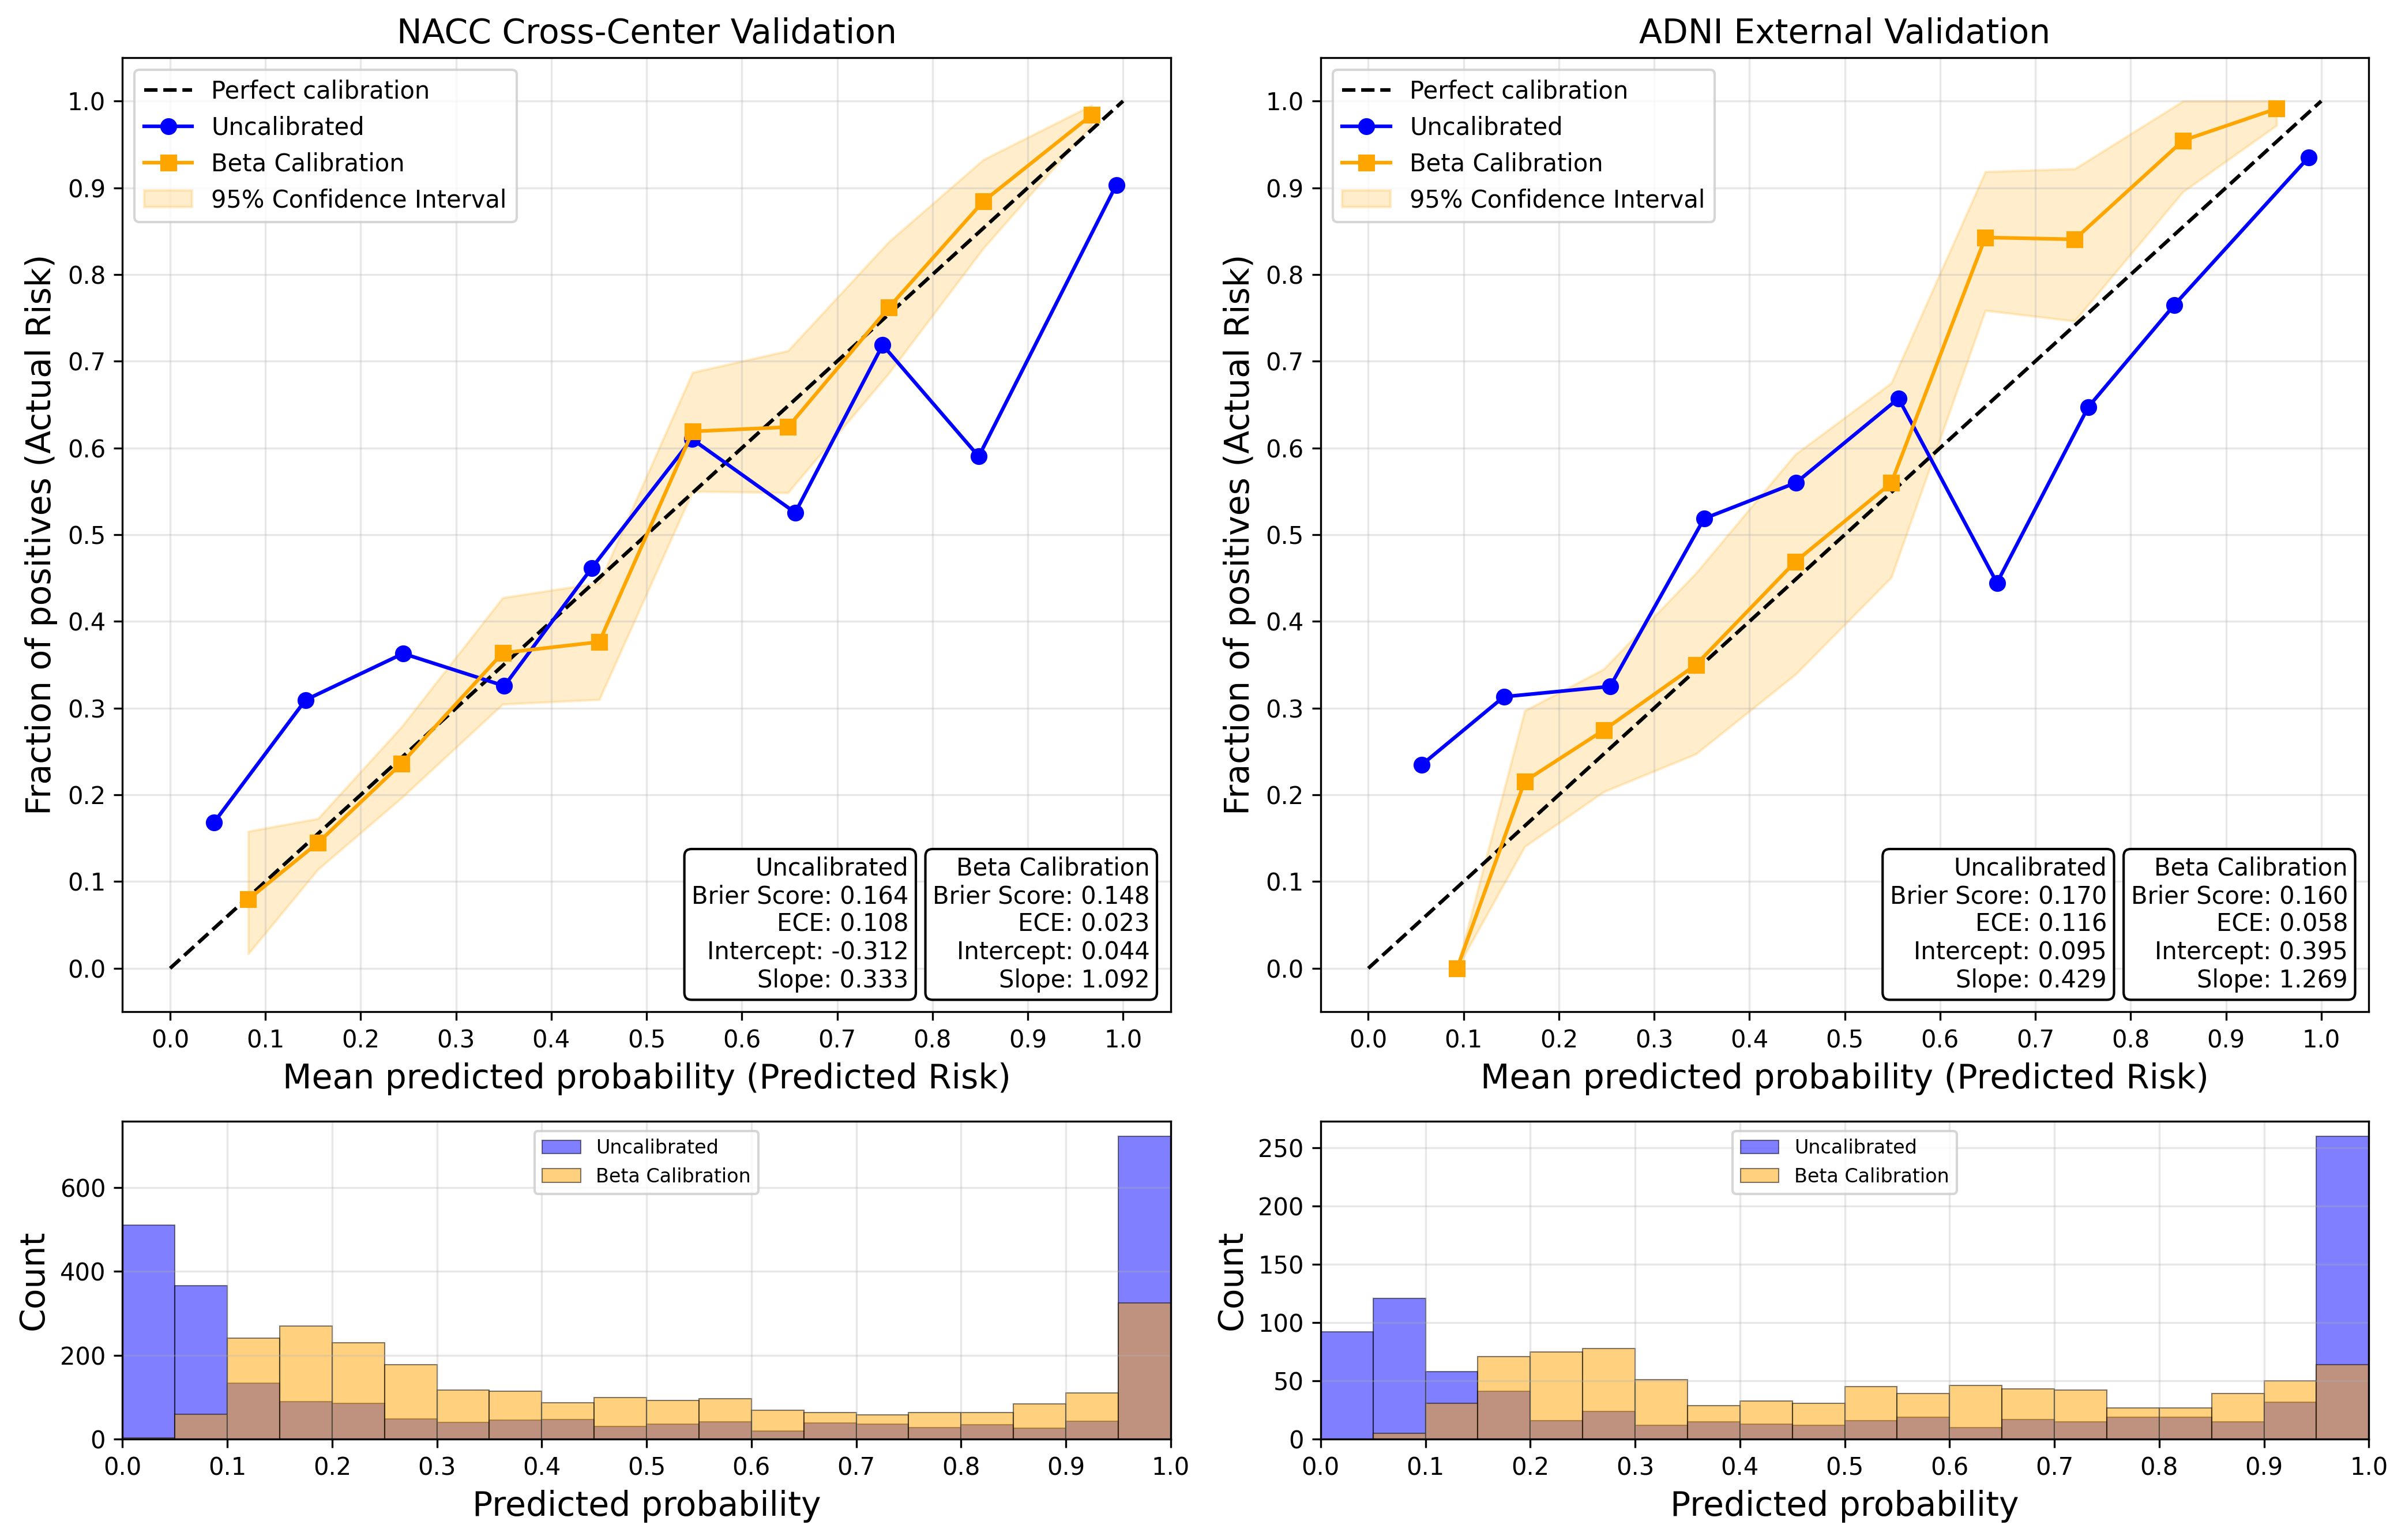
\includegraphics[width=1.0\textwidth]{figures/calibration/impaired_prediction_both_calibration_curve.png}
    \caption{Model calibration curves for the future NC vs. CI prediction task}
    \begin{minipage}{\textwidth}
      \footnotesize \hl{The horizontal axis shows the predicted probability and the vertical axis shows the observed frequency of the positive class. The diagonal line represents perfect calibration, and the curves compare the model before and after beta calibration.}
    \end{minipage}
    \label{fig:future_nc_ci_calib_curve}
\end{figure}

Similar improvements were observed in the ADNI external validation. Before calibration, the model produced extreme probabilities that did not correctly identify risk levels. The application of beta calibration successfully adjusted the spread of the predictions (slope = 1.269), although it resulted in underestimation of the CI risk in certain thresholds (intercept = 0.395). Overall, the calibration error was significantly reduced, as the ECE decreased from 0.116 to 0.058. This shows that the beta calibration method was able to successfully align the predicted probabilities with the actual results in both external validation datasets.

The excellent calibration of the LR model's predicted probabilities made the model highly valuable for clinical prediction of future CI. According to the DCA shown in Figure~\ref{fig:future_nc_ci_dca}, the model's net benefit exceeded that of the "treat all" and "treat none" strategies across a wide range of probability thresholds, specifically from 0.14 to 0.98 for the NACC cross-center validation and from 0.23 to 0.99 for the ADNI external validation. This result highlights that the LR model can provide clinical value in a wide range of risk threshold probabilities of future CI.

\begin{figure}[ht]
    \centering
    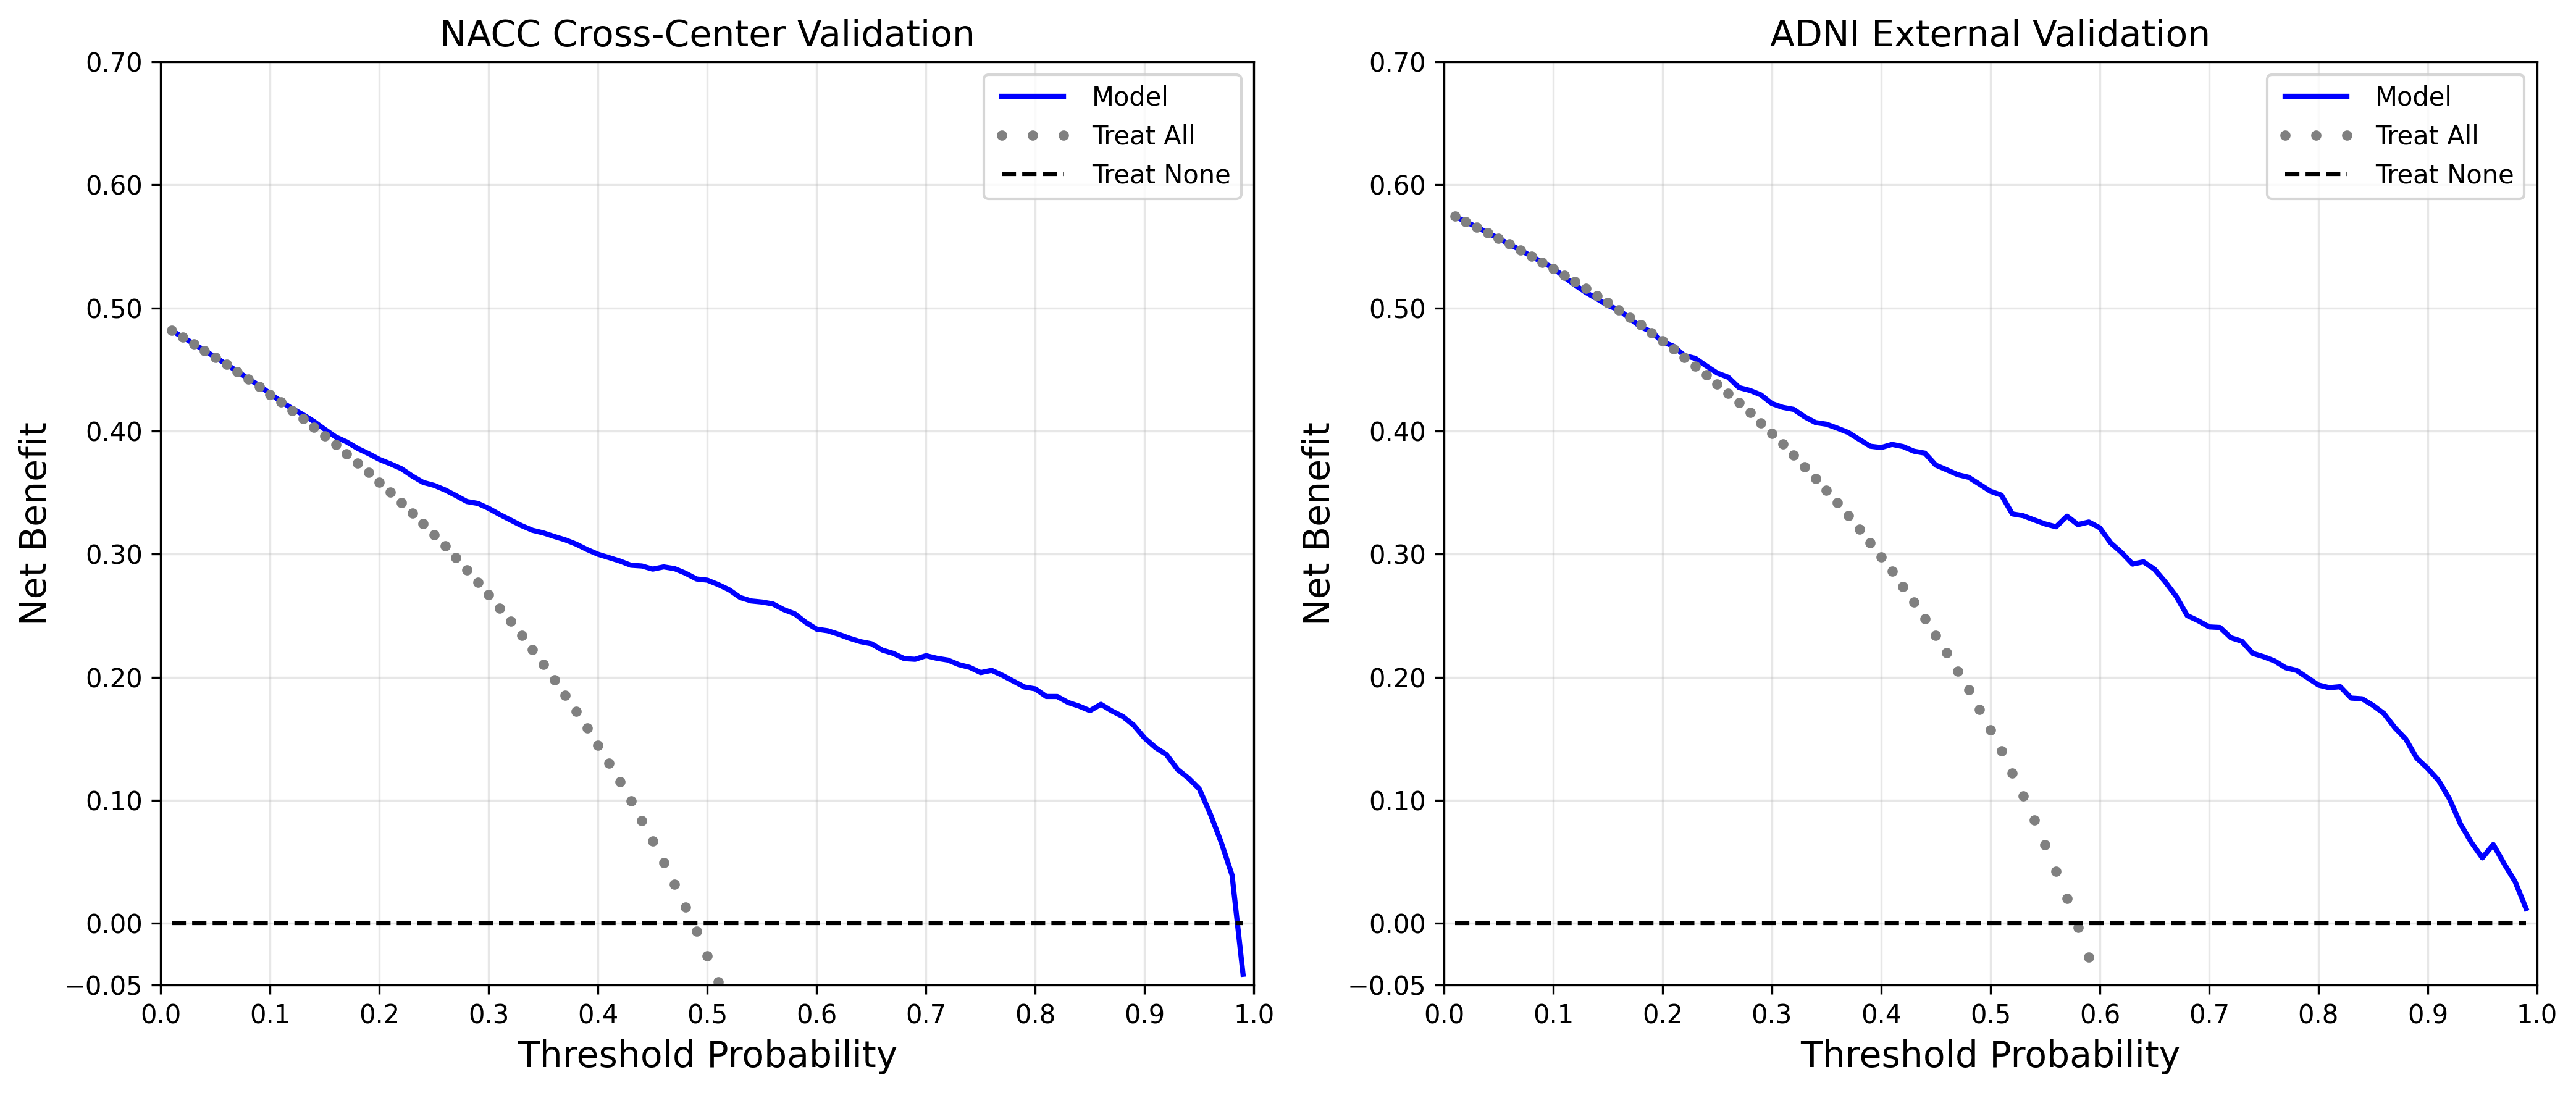
\includegraphics[width=1.0\textwidth]{figures/DCA/impaired_prediction_dca_both.png}
    \caption{The decision curve analysis (DCA) for the future NC vs. CI prediction task}
    \begin{minipage}{\textwidth}
      \footnotesize This figure illustrates the DCA curves of the NACC cross-center validation (left side) and the ADNI external validation (right side). "Treat All" refers to the assumption that all subjects are predicted to have CI in five years, and "Treat None" refers to the assumption that none of the subjects are predicted to have CI in five years.
    \end{minipage}
    \label{fig:future_nc_ci_dca}
\end{figure}

\subsubsection{External Validation Results for the Future CIND vs. Dementia Prediction Task}
The selected LR model for the future CIND vs. dementia prediction task was evaluated to determine its generalizability to unseen datasets. Table~\ref{tab:future_cind_dementia_results} provides a comparison of the model's performance in the internal cross-validation, NACC cross-center validation, and the ADNI external validation. The ROC curves for these validation stages are presented in Figure~\ref{fig:future_cind_dementia_roc}.

\begin{table}[!ht]
    \centering
    \caption{Performance of the selected logistic regression model in internal and external validation for the future CIND vs. dementia prediction task}
    \label{tab:future_cind_dementia_results}
    \newcolumntype{C}{>{\centering\arraybackslash}X}
        \begin{tabularx}{\textwidth}{|c|c|C|C|}
            \hline
            \textbf{Metric} & \textbf{Internal CV} & \textbf{NACC Cross-center Validation} & \textbf{ADNI External Validation} \\
            \hline
            AUC & \makecell{0.759 \\ {\small \hl{(0.751--0.768)}}} & \makecell{0.805 \\ {\small \hl{(0.784--0.828)}}} & \makecell{0.780 \\ {\small \hl{(0.740--0.819)}}} \\ \hline
            G-mean & 0.757 & 0.803 & 0.780 \\ \hline
            Sensitivity & 0.714 & 0.746 & 0.787 \\ \hline
            Specificity & 0.804 & 0.864 & 0.773 \\ \hline
            F1-score & 0.773 & 0.811 & 0.715 \\
            \hline
            \multicolumn{4}{p{400pt}}{\footnotesize \hl{AUC: area under the curve, F1-score: harmonic mean of precision and recall, G-mean: geometric mean score, Sensitivity: recall of the dementia class, Specificity: recall of the CIND class.}}
        \end{tabularx}
\end{table}

\begin{figure}[ht]
    \centering
    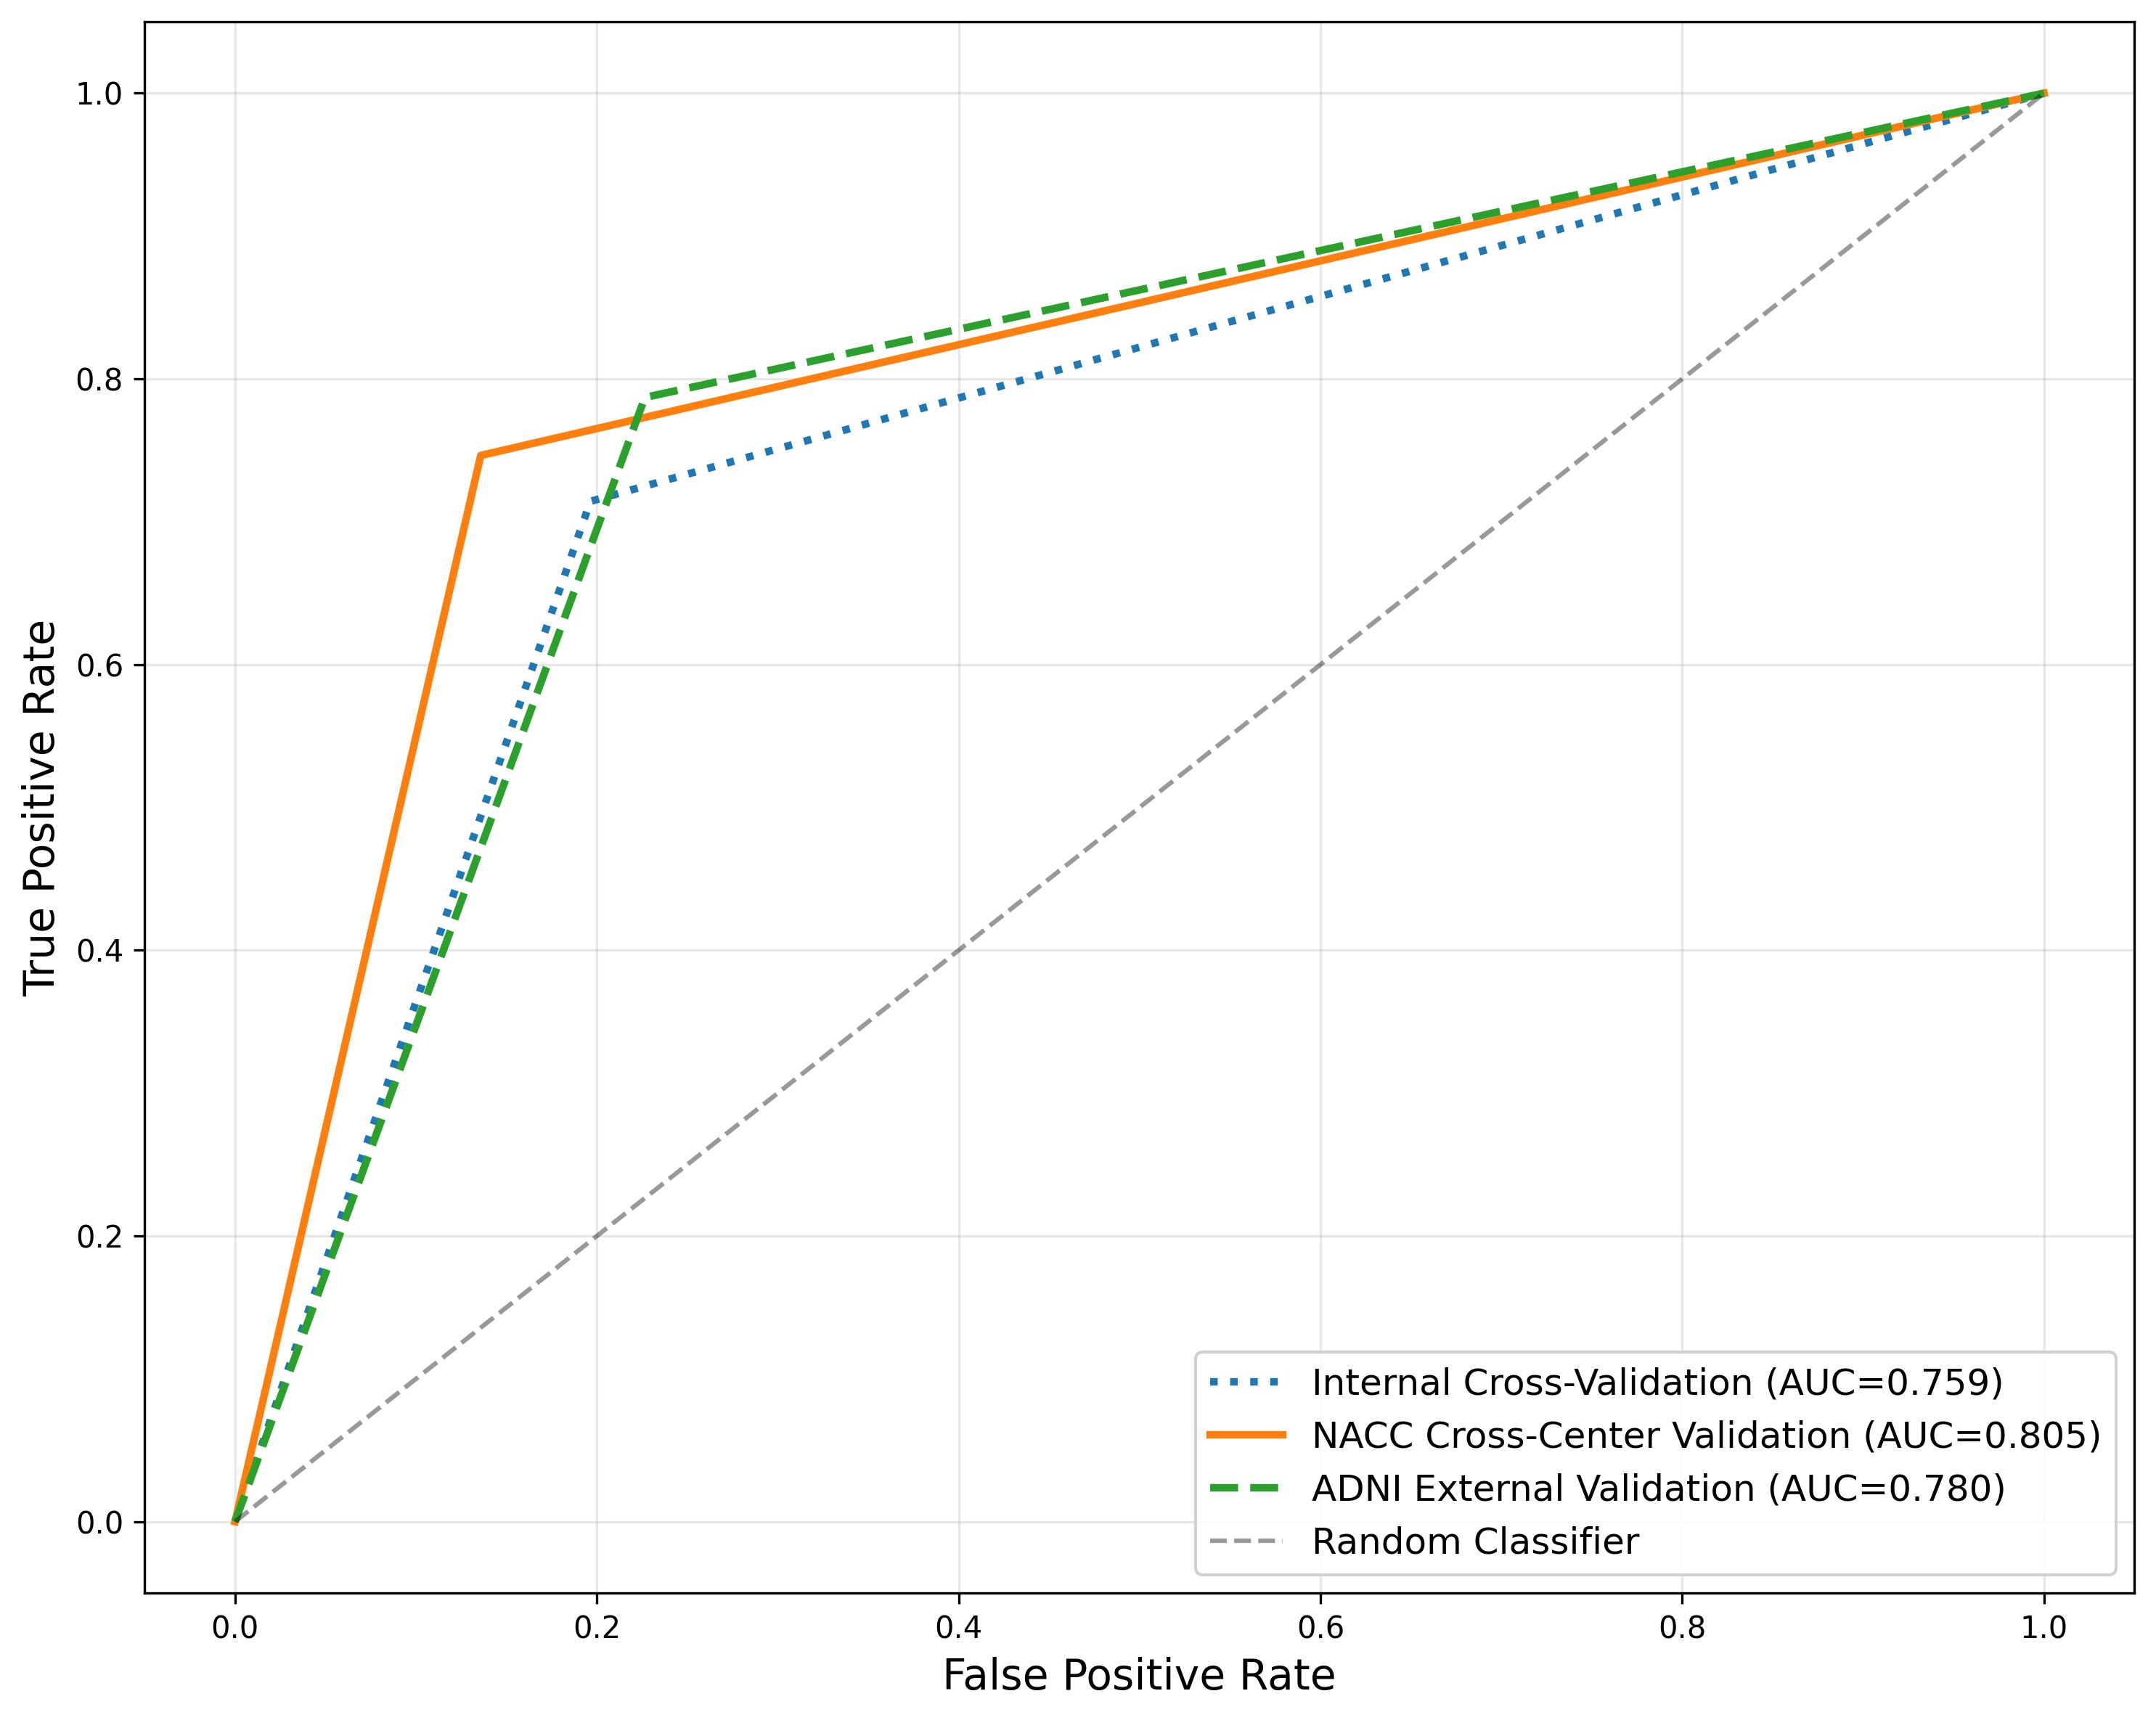
\includegraphics[width=0.7\textwidth]{figures/dementia_prediction_all_tests_roc_overlay.png}
    \caption{ROC curves comparing the performance of the logistic regression model for the future CIND vs. dementia prediction task}
    \begin{minipage}{\textwidth}
      \footnotesize \hl{The horizontal axis shows the false positive rate (1 -- specificity) and the vertical axis shows the true positive rate (sensitivity). Each curve represents one validation dataset.}
    \end{minipage}
    \label{fig:future_cind_dementia_roc}
\end{figure}

The LR model had a significant improvement in performance in the NACC cross-center validation compared to the internal CV. This result is similar to the previous prediction task. An improvement in sensitivity (0.714 to 0.746) and specificity (0.804 to 0.864) was observed. As a result, the AUC score increased from 0.759 to 0.805 and the G-mean increased from 0.757 to 0.803.  These results indicate that the model accurately generalized to the unseen data collected from different research.

The high generalizability of the LR model was also observed in the external validation on the ADNI dataset. The AUC score of 0.780 was higher than the internal CV baseline. This shows that the model can provide high classification performance even in a new clinical setting. A critical finding was noticed, which is the increase in sensitivity to 0.787. This is the highest sensitivity score across all three validation stages, indicating that the model is even more effective in correctly predicting future dementia risk in the ADNI cohort. 

In exchange for the increase in sensitivity, the LR model's specificity and F1-score dropped to 0.773 and 0.715, respectively. This drop in F1-score is largely driven by a significant reduction in precision (from 0.887 in the NACC cross-center validation to 0.655 in the ADNI external validation). This means that the model had a higher rate of false positives relative to true positives. Although a high number of false positives should be avoided, this result is in alignment with the clinical goal of a screening tool. In the context of predicting severe cognitive decline, it is safer for more patients to be flagged for further evaluation than missing actual cases of future dementia. Therefore, the model's ability to prioritize sensitivity on the external data supports its utility for early cognitive impairment prediction in real clinical practice. \hl{The improvement in AUC over the internal CV reached statistical significance in both validations (NACC cross-center p < 0.001, ADNI p = 0.016), which reflects the consistent gain observed in the external datasets.} The external validation results are reported with extended performance metrics in Table~\ref{table:lr-complete-perf-task4-apdx} in the appendix.

The selected LR model was calibrated to improve its estimation of future dementia risk. The calibration results for the external validation in the NACC and the ADNI datasets are shown in Figure~\ref{fig:future_cind_dementia_calib_curve}. In the NACC cross-center validation, the uncalibrated model assigned underestimated probabilities to subjects with moderate and low risk of dementia, while extreme probabilities were assigned to subjects with high risk. Using beta calibration, the spread of the probabilities was corrected (slope = 1.264), and the underestimation bias was reduced, especially in moderate risk thresholds (intercept = 0.111). As a result, the model calibration error (ECE) improved from 0.103 to 0.074, and the Brier score decreased from 0.149 to 0.139. Although the model's prediction improved, the model was still slightly miscalibrated as compared to the calibrated model in the future NC vs. CI prediction task.

\begin{figure}[ht]
    \centering
    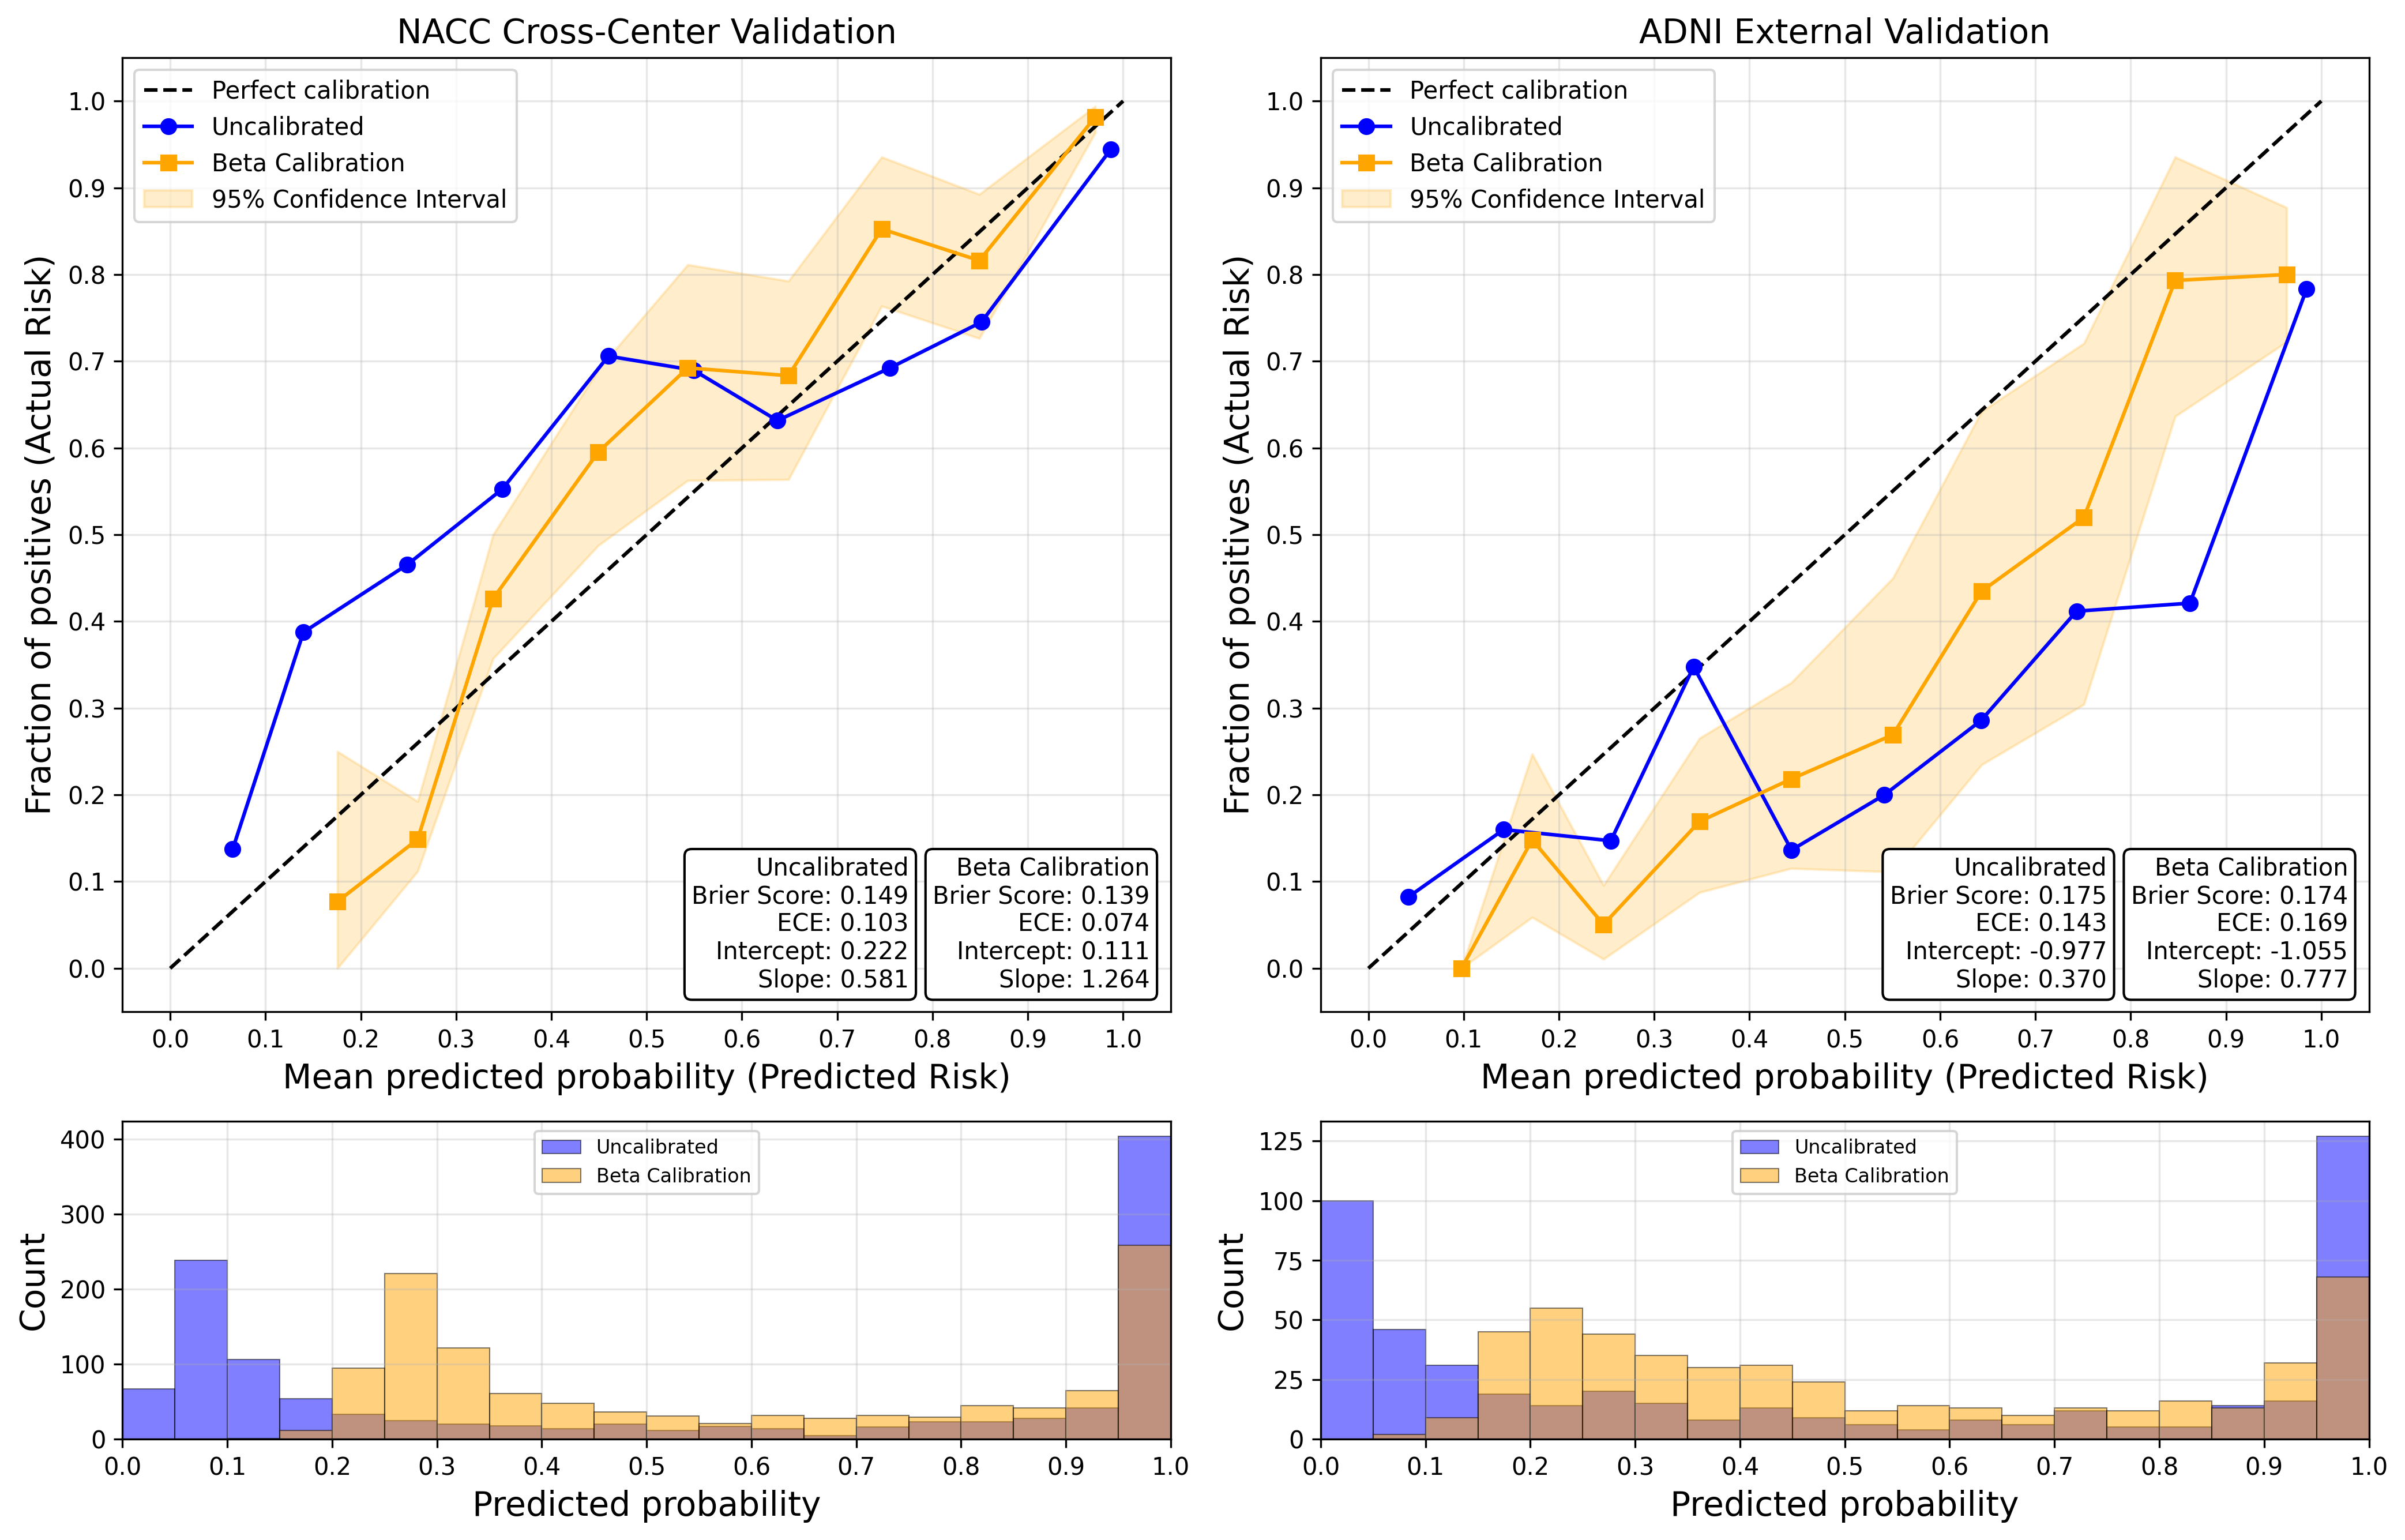
\includegraphics[width=1.0\textwidth]{figures/calibration/dementia_prediction_both_calibration_curve.png}
    \caption{Model calibration curves for the future CIND vs. dementia prediction task}
    \begin{minipage}{\textwidth}
      \footnotesize \hl{The horizontal axis shows the predicted probability and the vertical axis shows the observed frequency of the positive class. The diagonal line represents perfect calibration, and the curves compare the model before and after beta calibration.}
    \end{minipage}
    \label{fig:future_cind_dementia_calib_curve}
\end{figure}

The calibration results in the ADNI external validation were undesirable. In this dataset, the uncalibrated model severely overestimated the risk of dementia (intercept = -0.977). beta calibration could not fix the overestimation bias; instead, the ECE increased from 0.143 to 0.169. Applying the internal calibration parameters to the ADNI external data caused a mismatch between the predicted probabilities and the actual risk. The instability of the model predicted probabilities can be observed from the large confidence interval.

An evaluation of the clinical utility of the calibrated LR model was conducted using DCA as presented in Figure~\ref{fig:future_cind_dementia_dca}. The calibration of the model prediction improved the model's net benefit in the NACC cross-center validation, which outperformed the "treat all" and "treat none" strategies for the probability thresholds between 0.20 and 0.99. In contrast, the net benefit of the model was limited between the 0.18 and 0.79 thresholds in the ADNI external validation. Although the model demonstrated better clinical utility than the default strategies in the ADNI external, especially in low and intermediate thresholds, the DCA reflects the miscalibration of the model prediction observed in the calibration curve (intercept = -1.055).

\begin{figure}[ht]
    \centering
    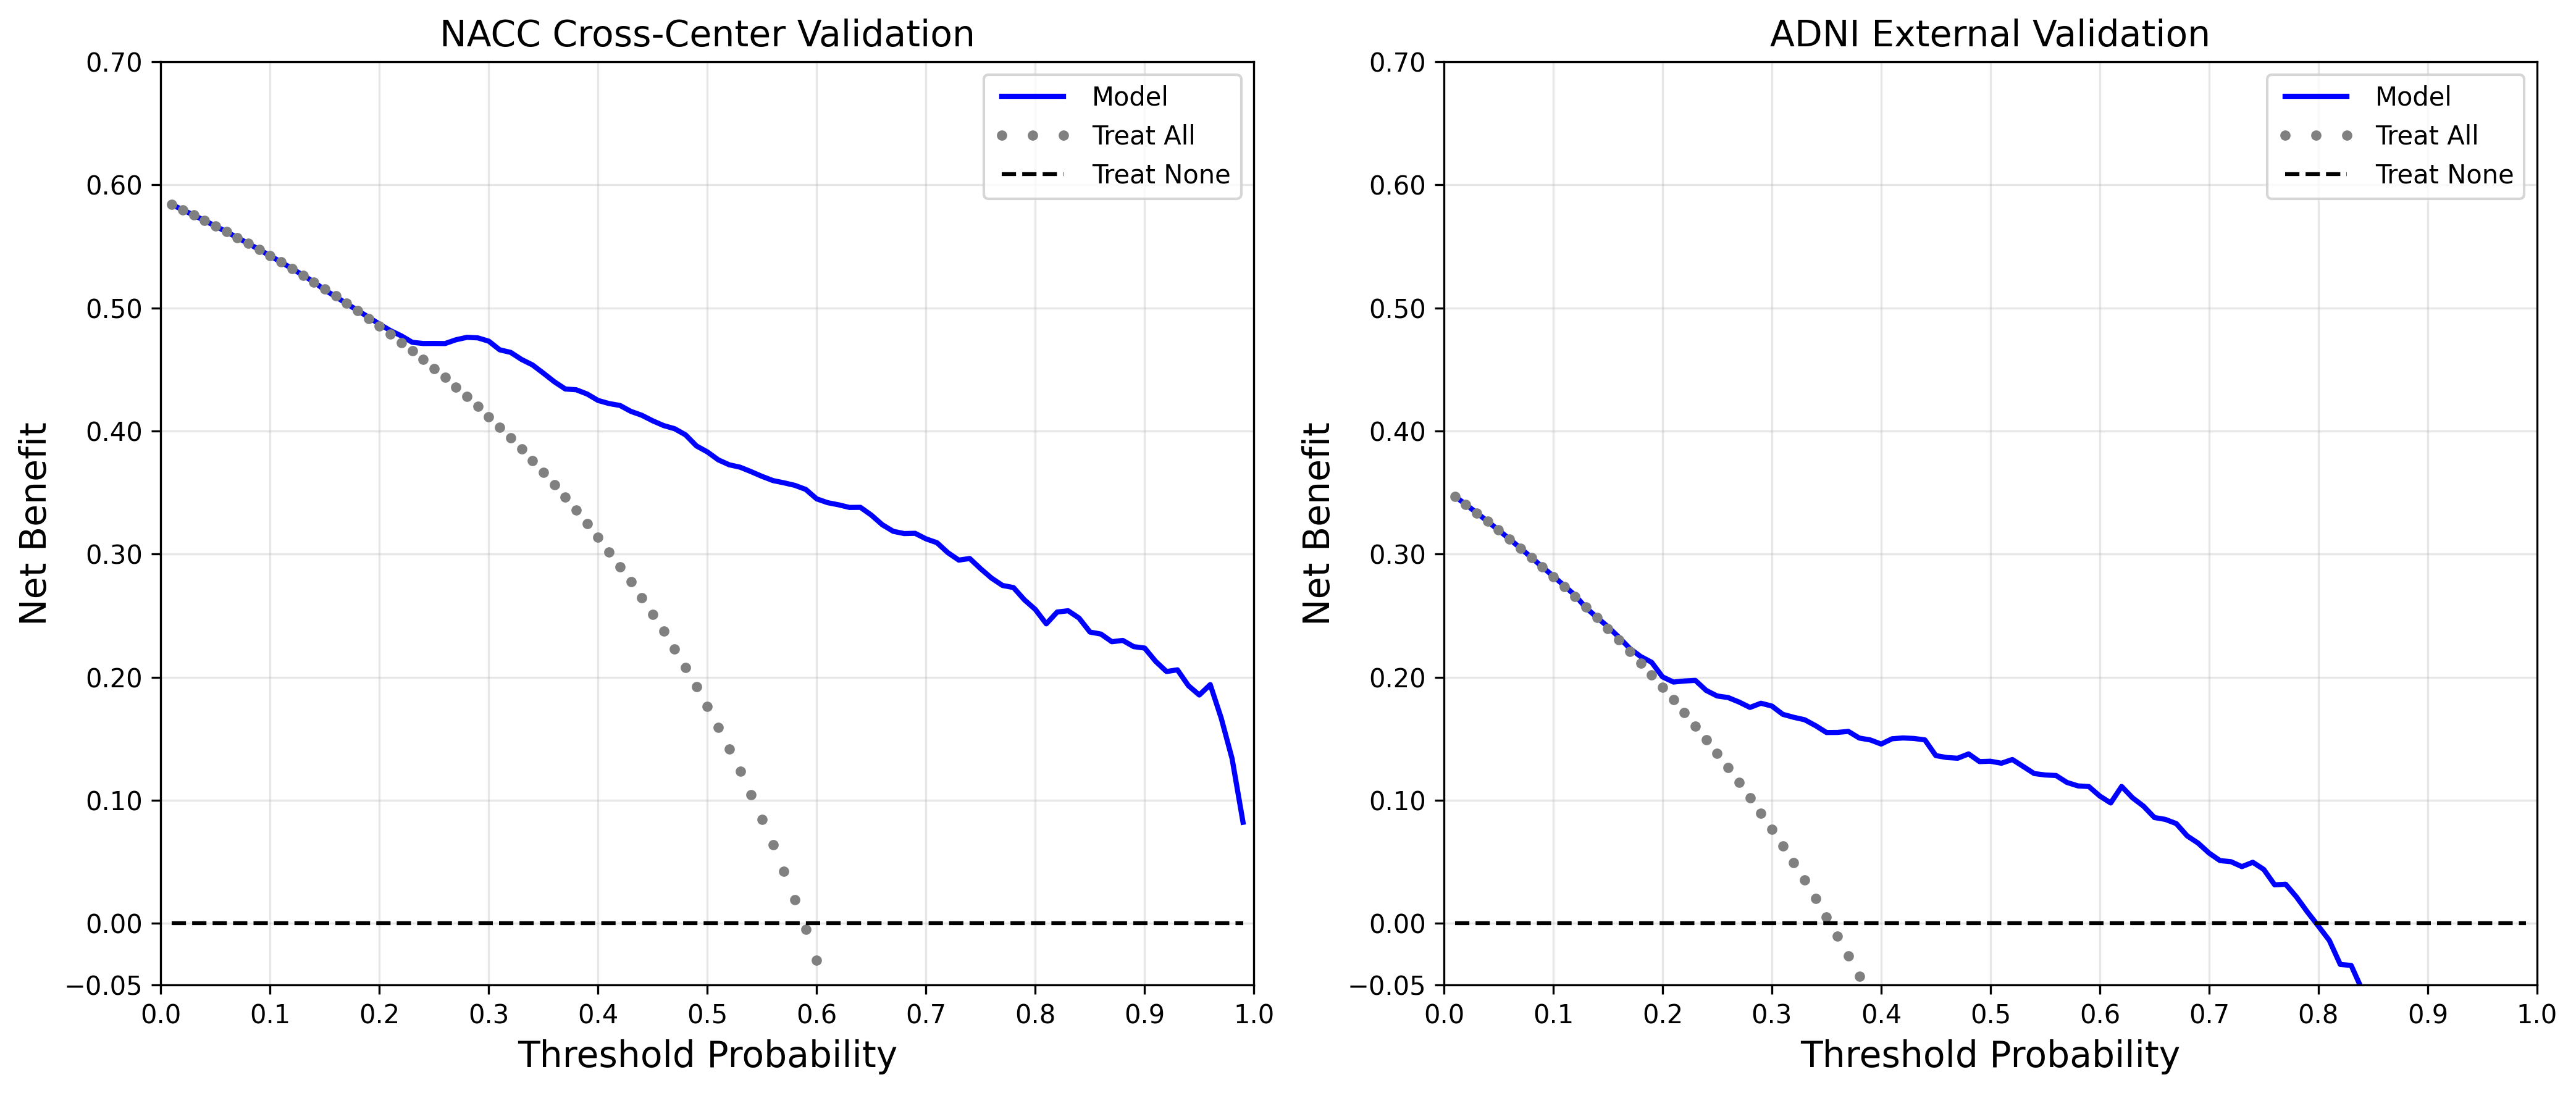
\includegraphics[width=1.0\textwidth]{figures/DCA/dementia_prediction_dca_both.png}
    \caption{The decision curve analysis (DCA) for the future CIND vs. dementia prediction task}
    \begin{minipage}{\textwidth}
      \footnotesize This figure illustrates the DCA curves of the NACC cross-center validation (left side) and the ADNI external validation (right side). "Treat All" refers to the assumption that all subjects are predicted to have dementia in five years, and "Treat None" refers to the assumption that all subjects are predicted to have CIND in five years.
    \end{minipage}
    \label{fig:future_cind_dementia_dca}
\end{figure}

The external validation results confirm that the developed models for predicting future cognitive status are generalizable. Both prediction models achieved high performance in the ADNI study, especially in detecting cases with high risk (sensitivity). The models also scored high accuracy in the NACC cross-center validation compared to the internal CV. In addition, the models presented excellent calibration and clinical utility to accurately estimate the risk of CI and dementia, especially in the NACC cross-center validation. These results validate the second objective of the study, demonstrating that accessible baseline data can be used to effectively predict the risk of cognitive impairment up to five years in the future across diverse clinical settings.

\subsection{Model Explainability Results}

\subsubsection{Model Explainability Results for the Future NC vs. CI Prediction Task}
The features in the future prediction of NC vs. CI are ranked according to their global importance in Figure~\ref{figure:nc_ci_prediction_feature_importance}. A similar feature importance ranking can be observed in both the NACC cross-center validation and the ADNI external validation. This is confirmed by the Spearman’s rank correlation coefficient of 0.83 ($p$ < 0.05). In both tests, the model relied heavily on a combination of functional activities, self-reported memory issues (MEMPROB), and behavioral factors (IRR). The feature representing self-reported memory issues was identified as the most important predictor. The only notable difference in the feature importance of the two external validation was the SHAP value of the IRR feature. It was observed that the IRR feature has a significantly higher influence on the model prediction in the ADNI external validation compared to the NACC cross-center validation.

\begin{figure}[ht]
    \centering
    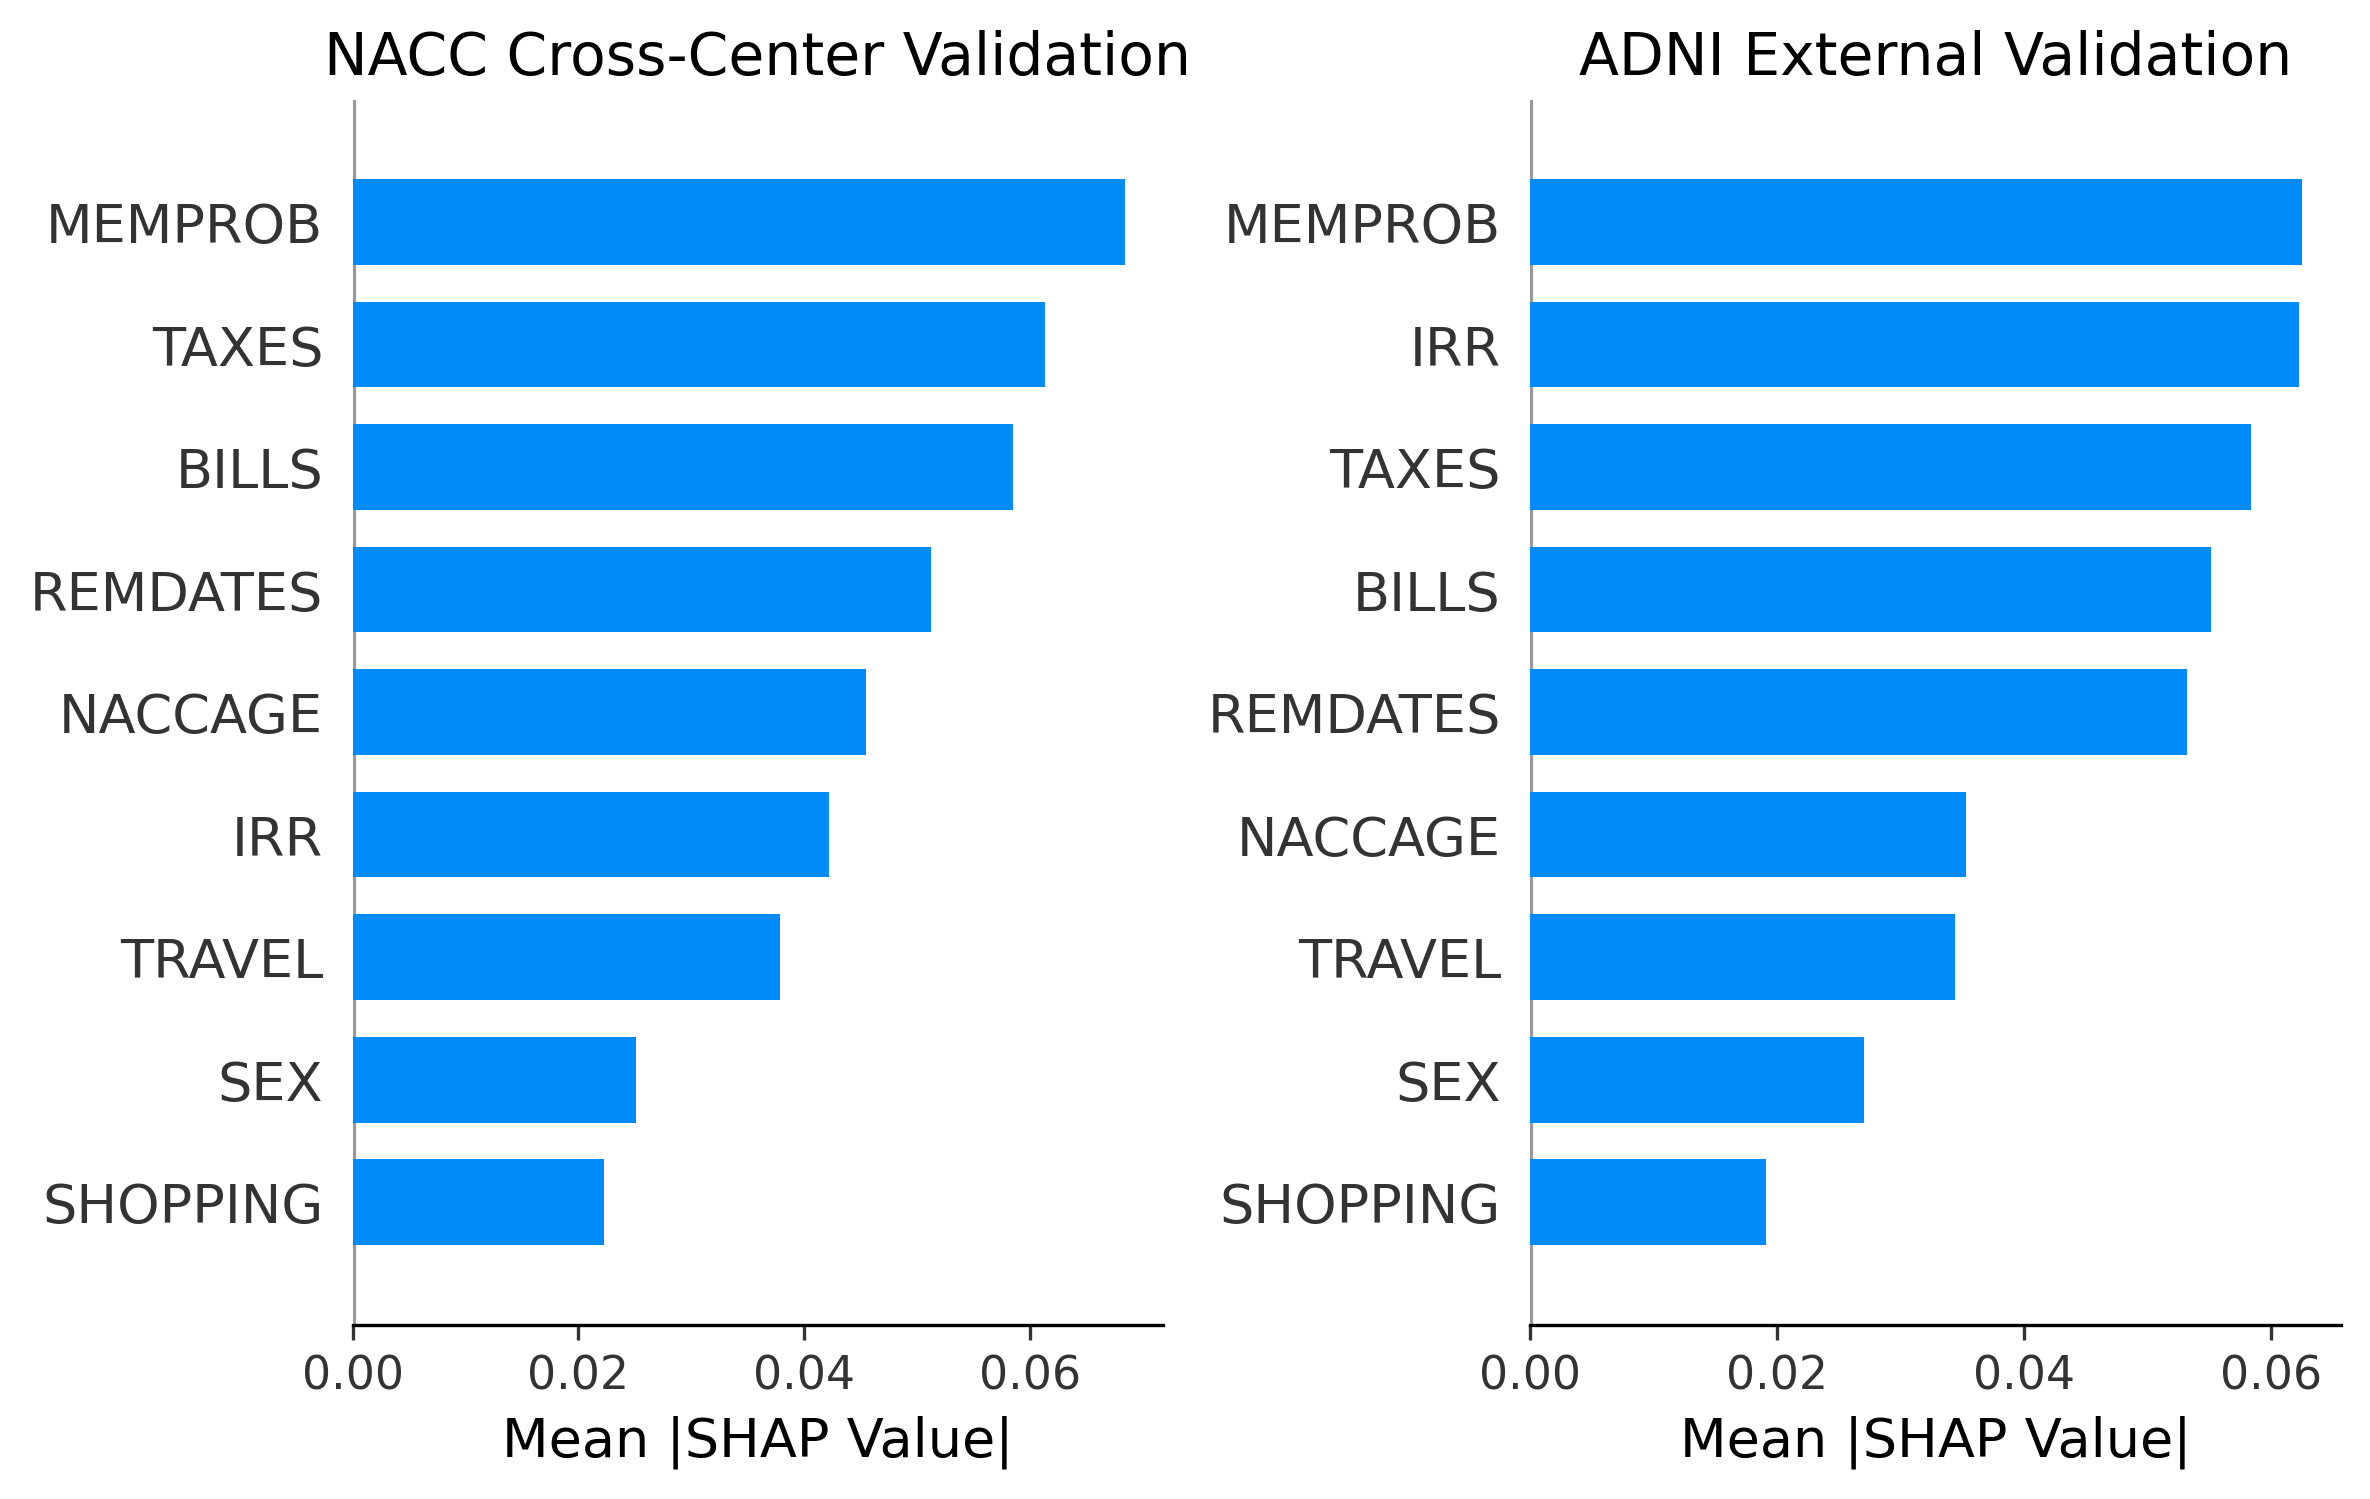
\includegraphics[width=1.0\textwidth]{figures/XAI/impaired_prediction_both_feature_importance_comparison.png}
    \caption{Feature importance in the NACC cross-center validation and the ADNI external validation for the future NC vs. CI prediction task}
    \begin{minipage}{\textwidth}
      \footnotesize \hl{The bars represent the mean absolute SHAP value of each feature, which ranks the contribution of the feature to the model prediction in the two validation datasets.}
    \end{minipage}
    \label{figure:nc_ci_prediction_feature_importance}
\end{figure}

Analyzing the local explanation of the selected model is crucial, as subjects with different risk profiles might have similar prediction outcomes. Figure~\ref{figure:nc_ci_prediction_pos_waterfall} demonstrates two correctly predicted CI instances with the same probabilities of 55\%. The demographic characteristics (male gender and older age of 79 years), together with a history of never performing tax-related tasks (TAXES), were the main risk factors of CI for Instance A. In contrast, \textit{Instance B} has a different risk profile mainly associated with difficulty remembering dates and appointments (REMDATES).

\begin{figure}[ht]
    \centering
    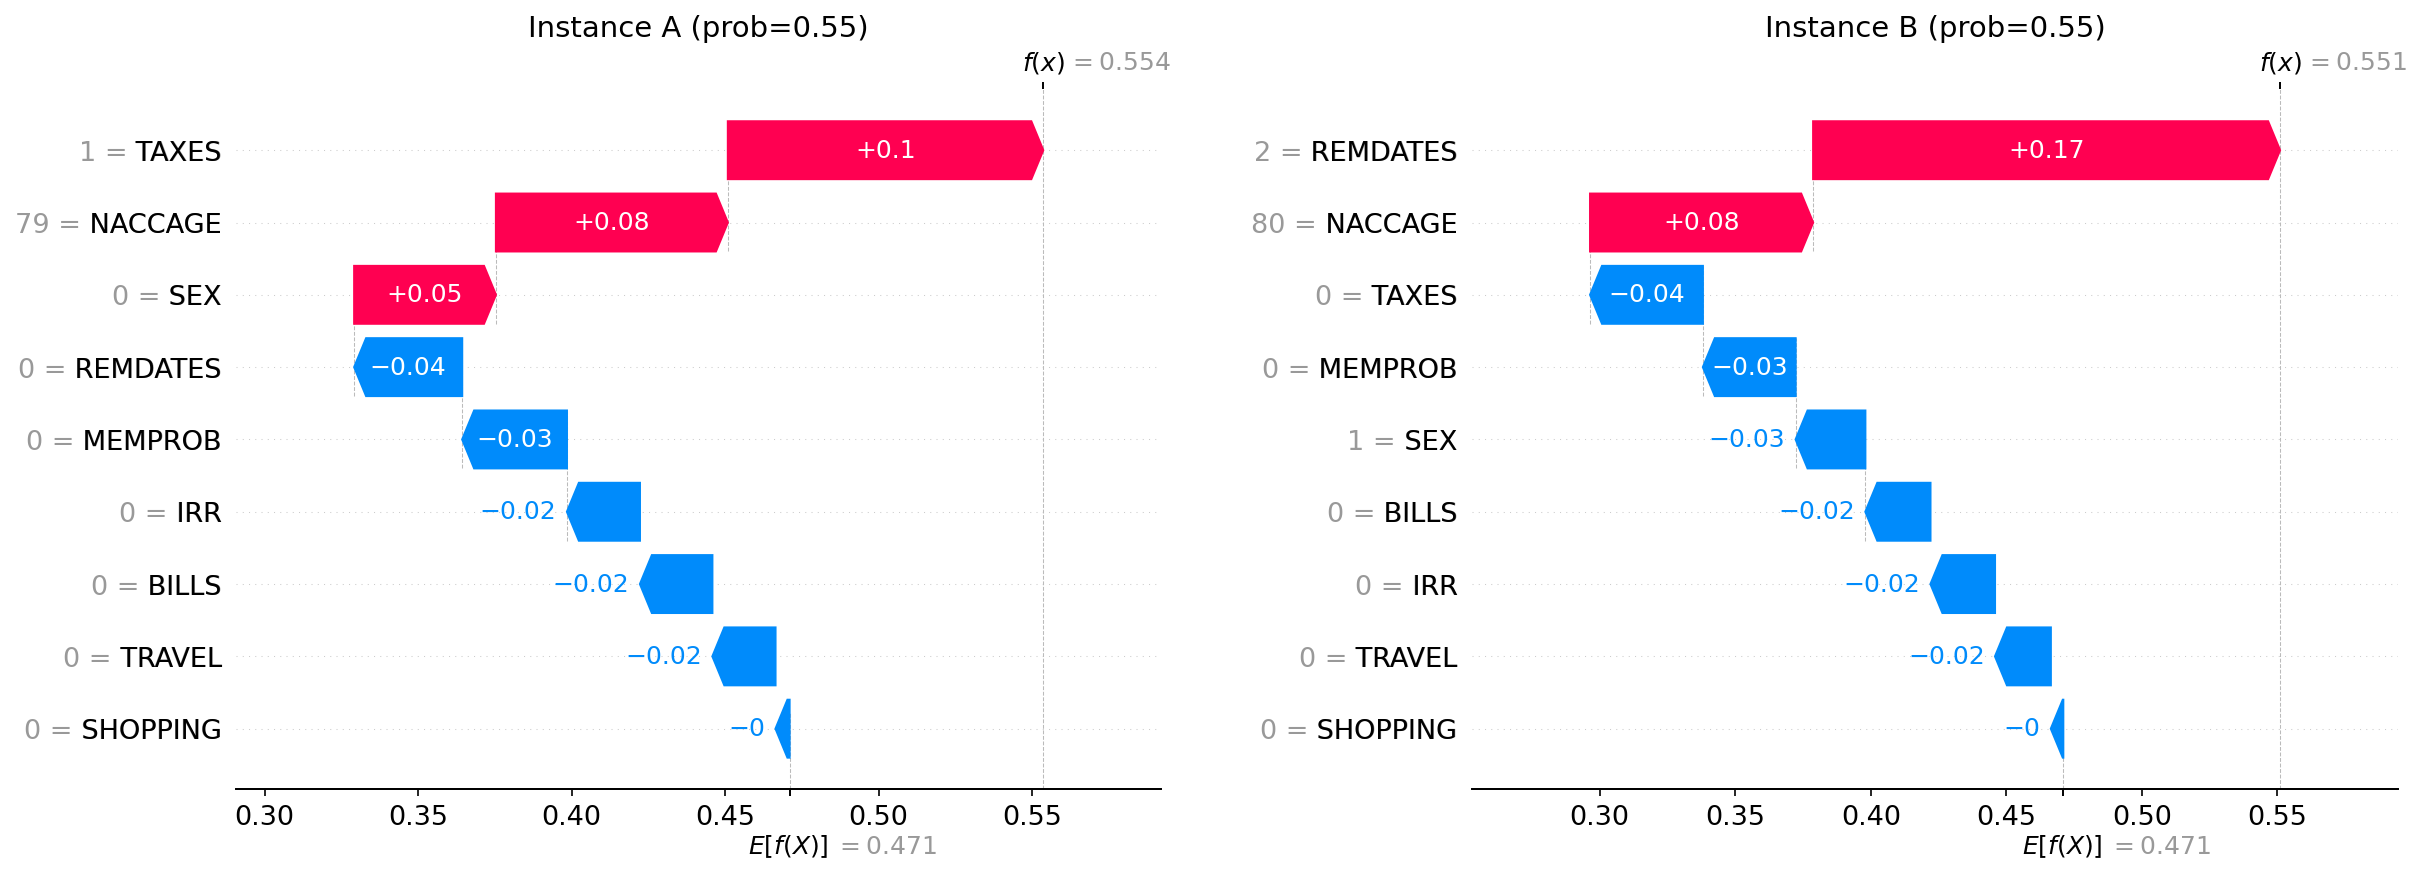
\includegraphics[width=1.0\textwidth]{figures/XAI/impaired_prediction_adni_true_positive_waterfall.png}
    \caption{SHAP waterfall plots for two instances correctly predicted as having risk of cognitive impairment within five years in future}
    \begin{minipage}{\textwidth}
      \footnotesize \hl{The plot shows how the value of each feature shifts the prediction from the base value to the final predicted probability for a single instance.}
    \end{minipage}
    \label{figure:nc_ci_prediction_pos_waterfall}
\end{figure}

A similar analysis was also performed on two instances correctly predicted as NC. Figure~\ref{figure:nc_ci_prediction_neg_waterfall} displays the waterfall plots of both instances. \textit{Instance A} has a normal ability to perform all functional activities, which reduced the probability of developing CI despite the high demographic risk of being an 84-year-old male. The younger female subject represented by \textit{Instance B} has a similar protective functional profile, except she has never done a tax filing before. It is interesting that this instance is similar to \textit{Instance A} in Figure~\ref{figure:nc_ci_prediction_pos_waterfall}, correctly predicted as cognitively impaired, with sex being the only major difference. This contrast highlights how interaction between features can change the predictive risk of cognitive impairment.

\begin{figure}[ht]
    \centering
    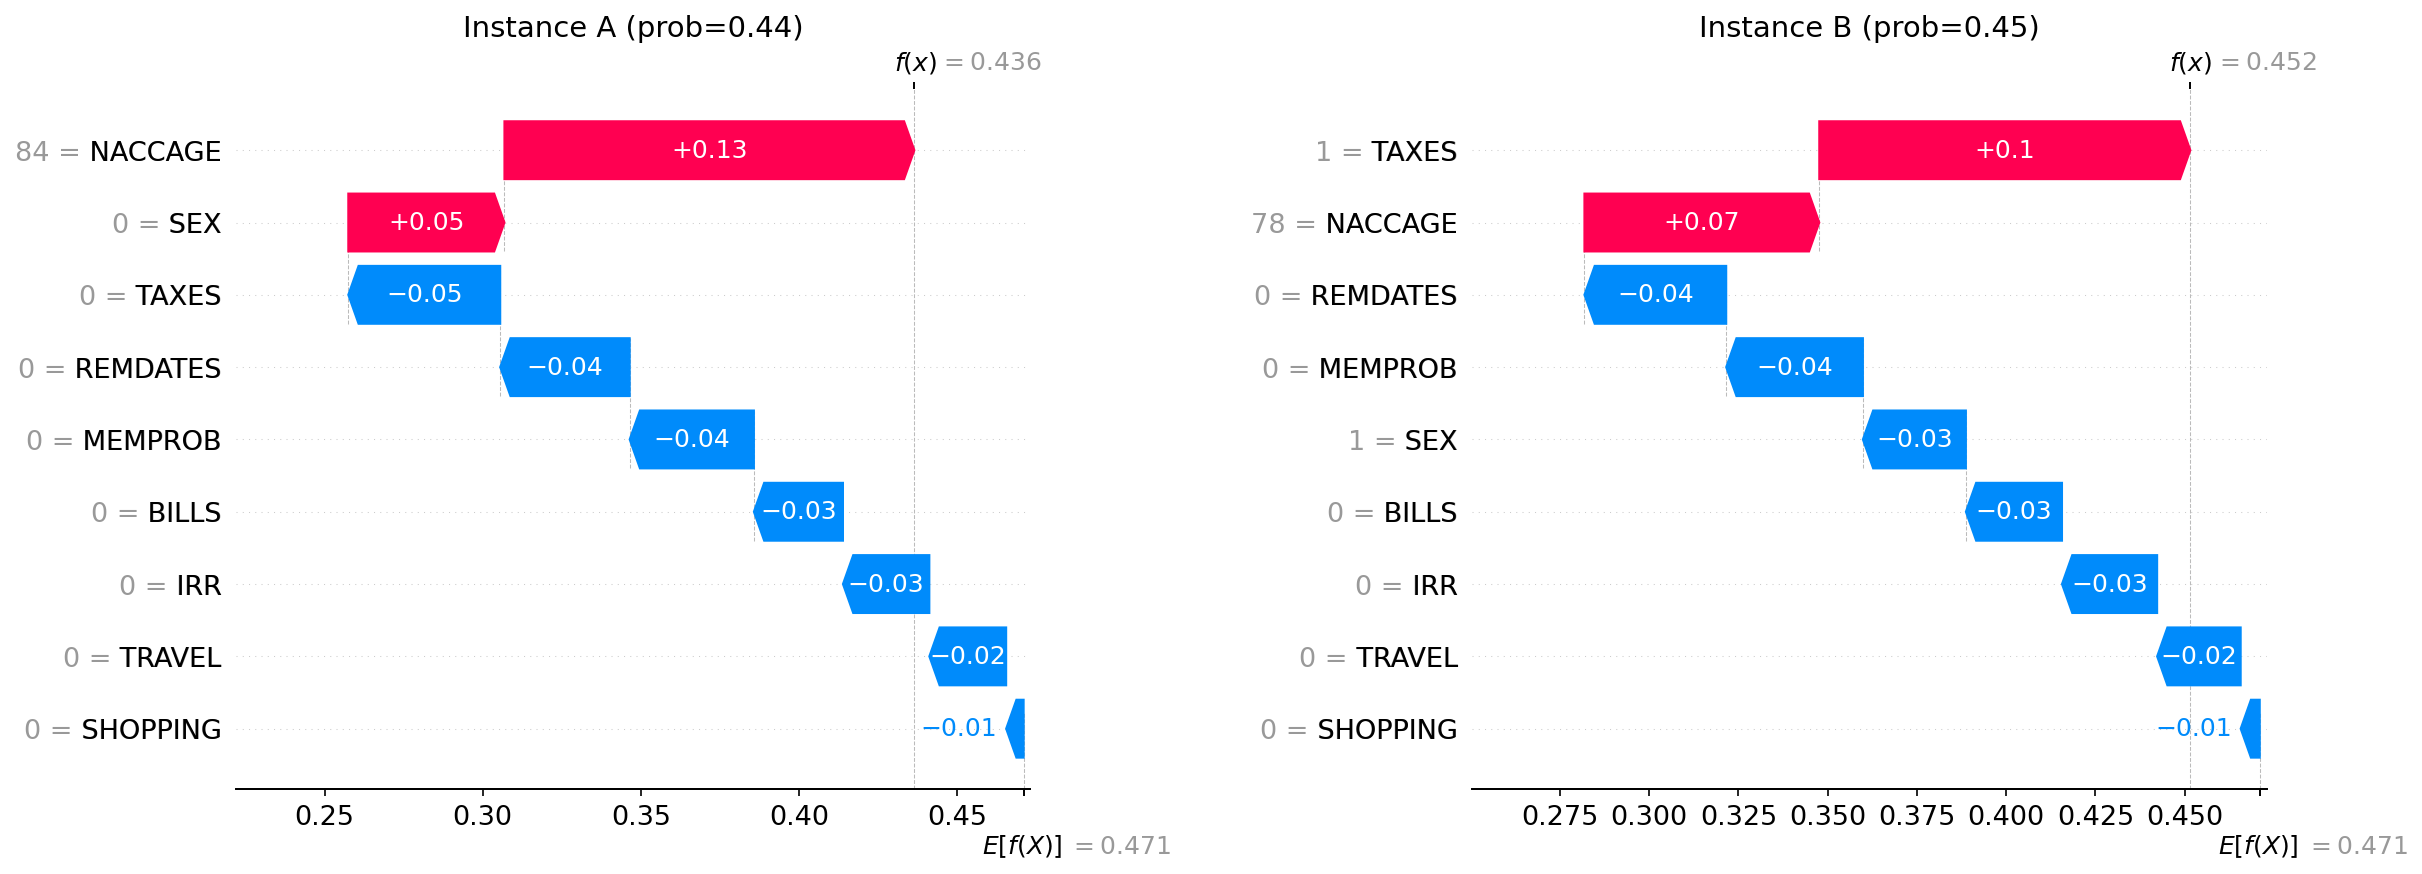
\includegraphics[width=1.0\textwidth]{figures/XAI/impaired_prediction_adni_true_negative_waterfall.png}
    \caption{SHAP waterfall plots for two instances correctly predicted as normal cognition within five years in future}
    \begin{minipage}{\textwidth}
      \footnotesize \hl{The plot shows how the value of each feature shifts the prediction from the base value to the final predicted probability for a single instance.}
    \end{minipage}
    \label{figure:nc_ci_prediction_neg_waterfall}
\end{figure}

The results of using DiCE to generate counterfactual examples are presented in Figure~\ref{figure:nc_ci_prediction_dice_stat}. DiCE had an excellent success rate in providing suggestions to prevent the potential CI risk early, with valid counterfactual examples generated for all ADNI external data instances. However, the range of risk prevention suggestions (counterfactual examples) available to each individual was more limited compared to the classification tasks presented in section \ref{sec:cls-xai}. On average, the majority of ADNI instances (69\%) receive only one valid suggestion to reverse their predicted prognosis from CI to NC.

\begin{figure}[ht]
    \centering
    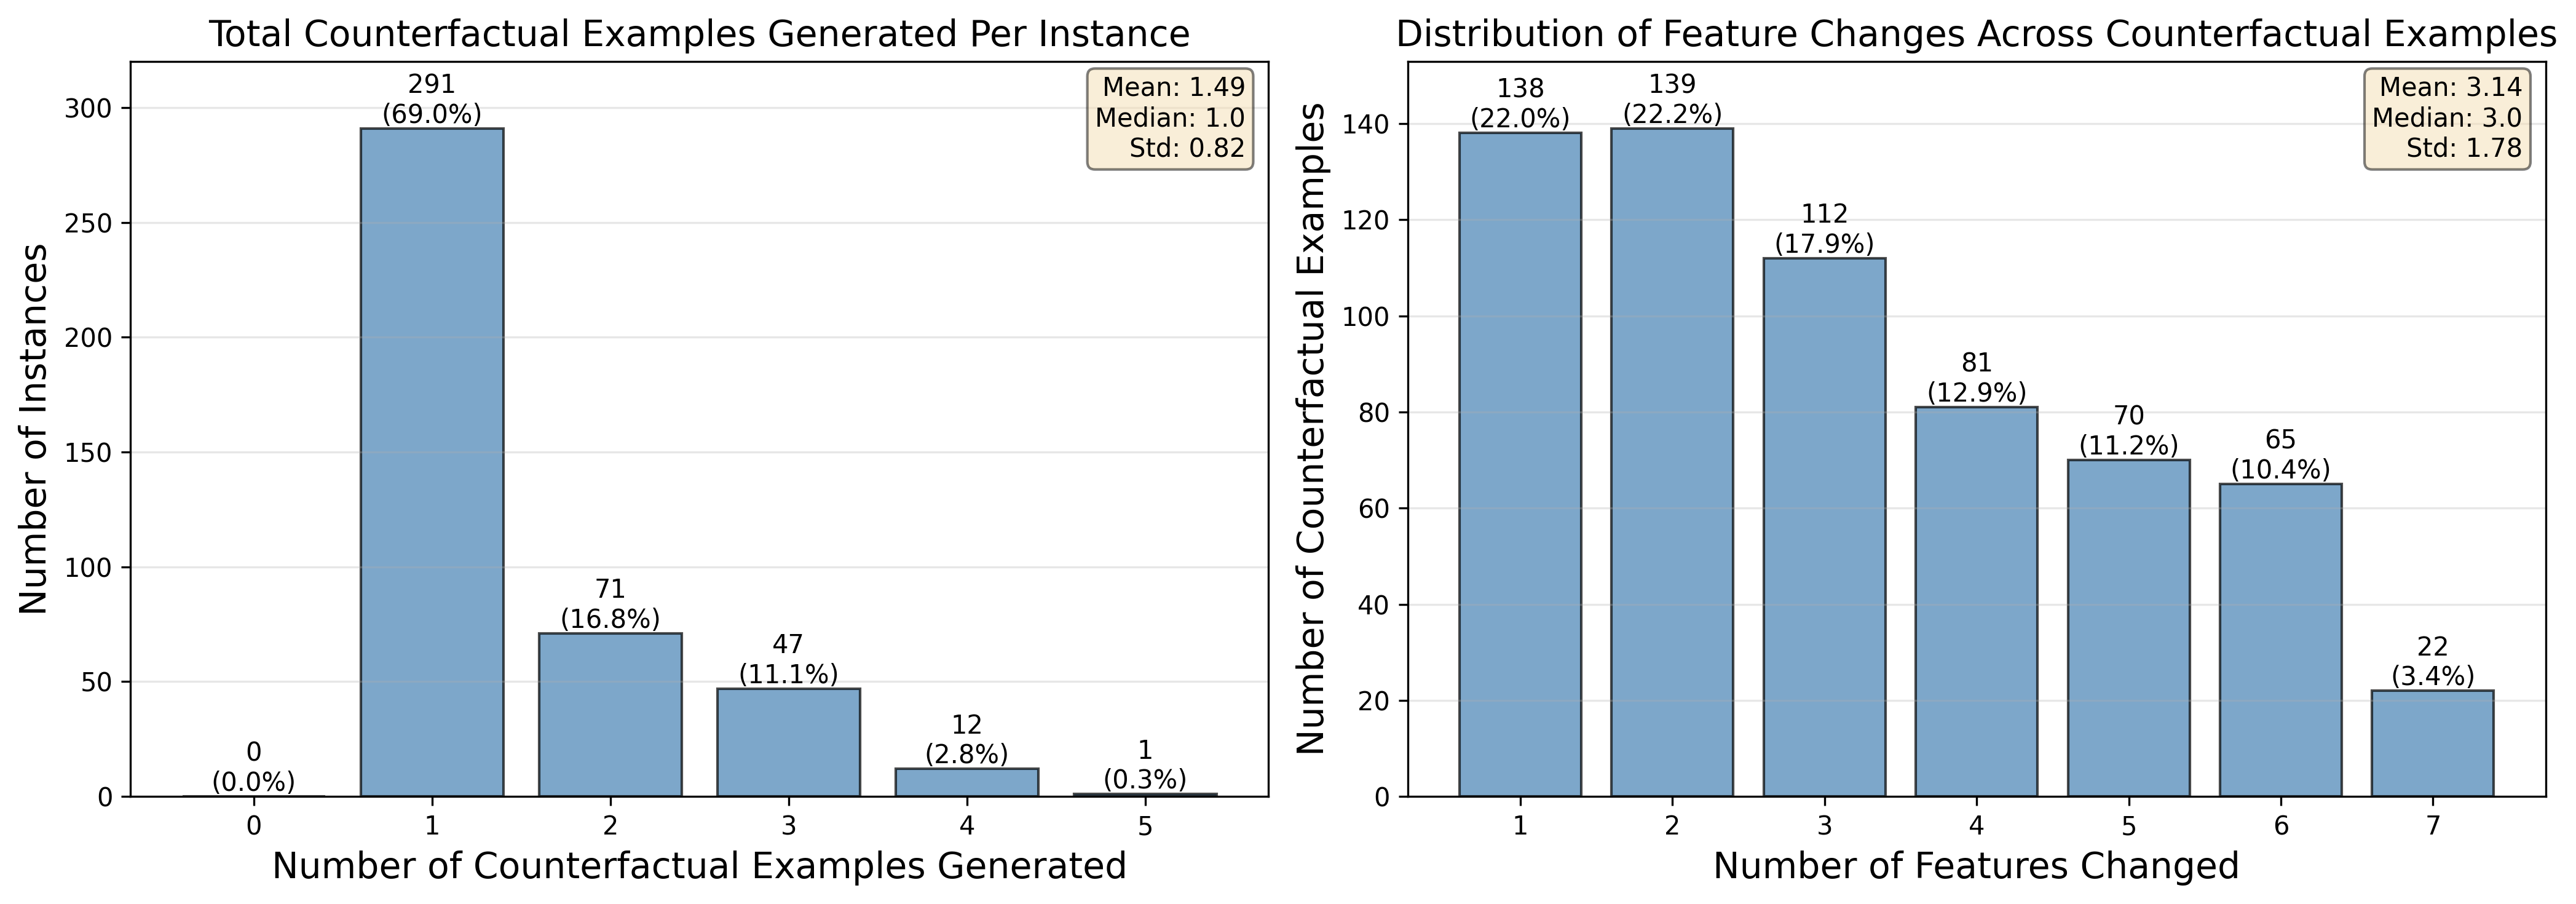
\includegraphics[width=1.0\textwidth]{figures/XAI/impaired_prediction_adni_kdtree_dice_stats.png}
    \caption{Summary of generated counterfactual examples for changing predicted risk from cognitive impairment to normal cognition}
    \label{figure:nc_ci_prediction_dice_stat}
\end{figure}

Regarding the feasibility of these interventions, the distribution of feature changes in Figure~\ref{figure:nc_ci_prediction_dice_stat} suggests that the risk of CI can be prevented early with minimal changes in risk factors. This is possible by modifying up to 3 of the 7 alterable features. According to the presented results, a significant proportion of the generated counterfactuals (44.2\%) required the change of only one or two features. This indicates that risk prevention plans that focus on a few risk factors could be enough to improve future cognitive status. The counterfactual explanation in the NACC cross-center validation had similar results with slightly higher feature changes required to generate the counterfactual examples. The results are presented in Figure~\ref{figure:dice-nacc-task3-apdx} in the appendix.

The most critical features that drive these interventions are ranked in Figure~\ref{figure:nc_ci_prediction_dice_feature_importance}. Remembering dates and appointments (REMDATES) was the most frequently modified feature (58\%), followed closely by handling taxes (TAXES, 55\%) and paying bills (BILLS, 52\%). Behavioral conditions were also found to be one of the key intervention factors in the ADNI external validation, with irritability (IRR) being modified in 51\% of the cases. Table~\ref{table:cfe-adni-task3-apdx} in the appendix presents counterfactual examples that illustrate how the feature values of a random subject with a future predicted risk of CI can be changed to prevent the risk.

\begin{figure}[ht]
    \centering
    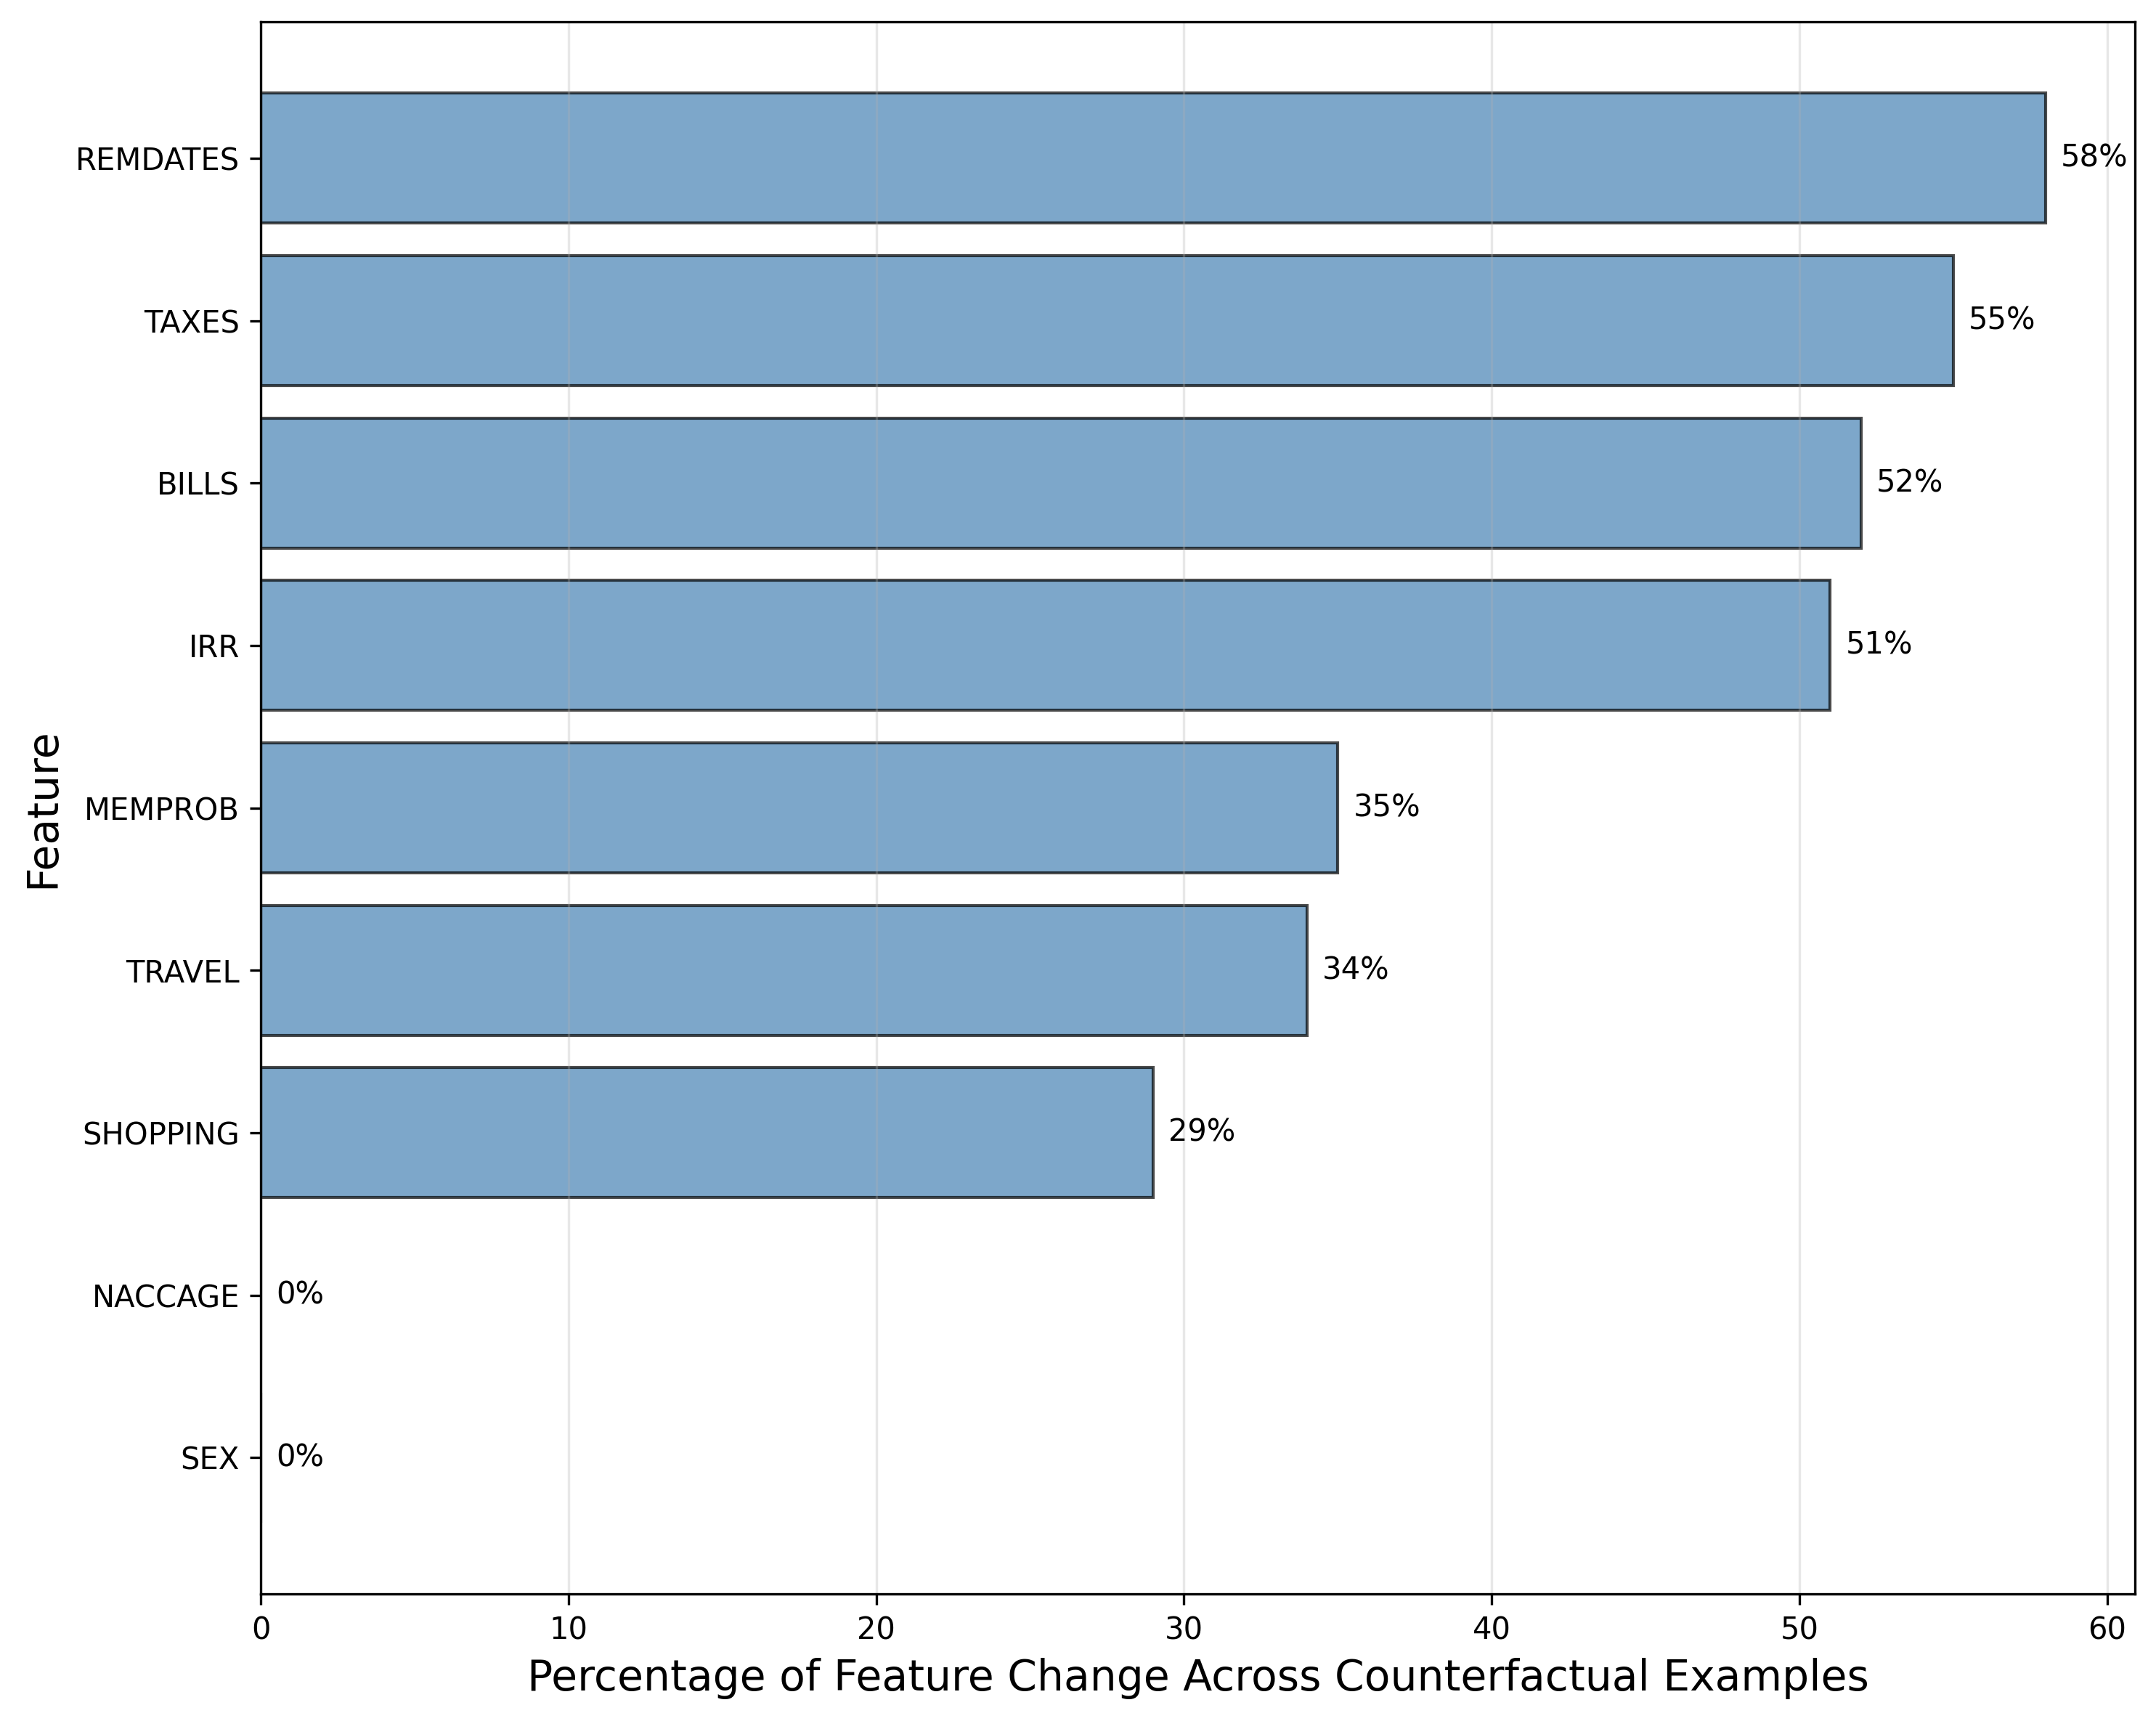
\includegraphics[width=1.0\textwidth]{figures/XAI/impaired_prediction_adni_kdtree_dice_global_importance.png}
    \caption{Feature importance ranking based on counterfactual explanations for the future NC vs. CI prediction task}
    \begin{minipage}{\textwidth}
      \footnotesize The features are ranked based on the percentage of times they were modified to generate valid counterfactual examples. The rank highlights the most critical features for risk intervention. Demographic features (NACCAGE and SEX) show 0\% importance because they were set as invariable features in the counterfactual generation process.
    \end{minipage}
    \label{figure:nc_ci_prediction_dice_feature_importance}
\end{figure}

\subsubsection{Model Explainability Results for the Future CIND vs. Dementia Prediction Task}
The global feature importance ranking of this prediction task is demonstrated in Figure~\ref{figure:cind_dementia_prediction_feature_importance}. The ranking of features is significantly similar in both the NACC cross-center validation and the ADNI external validation. This similarity is measured by Spearman’s rank correlation coefficient of 0.98 ($p$ < 0.05). In both cohorts, the model’s prediction was strongly influenced by measures of functional activities, specifically the ability to manage financial matters (BILLS and TAXES). The difficulty in remembering dates (REMDATES) and traveling (TRAVEL) also have high SHAP values. These results were observed in other classification and prediction tasks. In contrast, body mass index (NACCBMI) and symptoms such as energy levels (ENERGY) showed considerably lower importance scores.

\begin{figure}[ht]
    \centering
    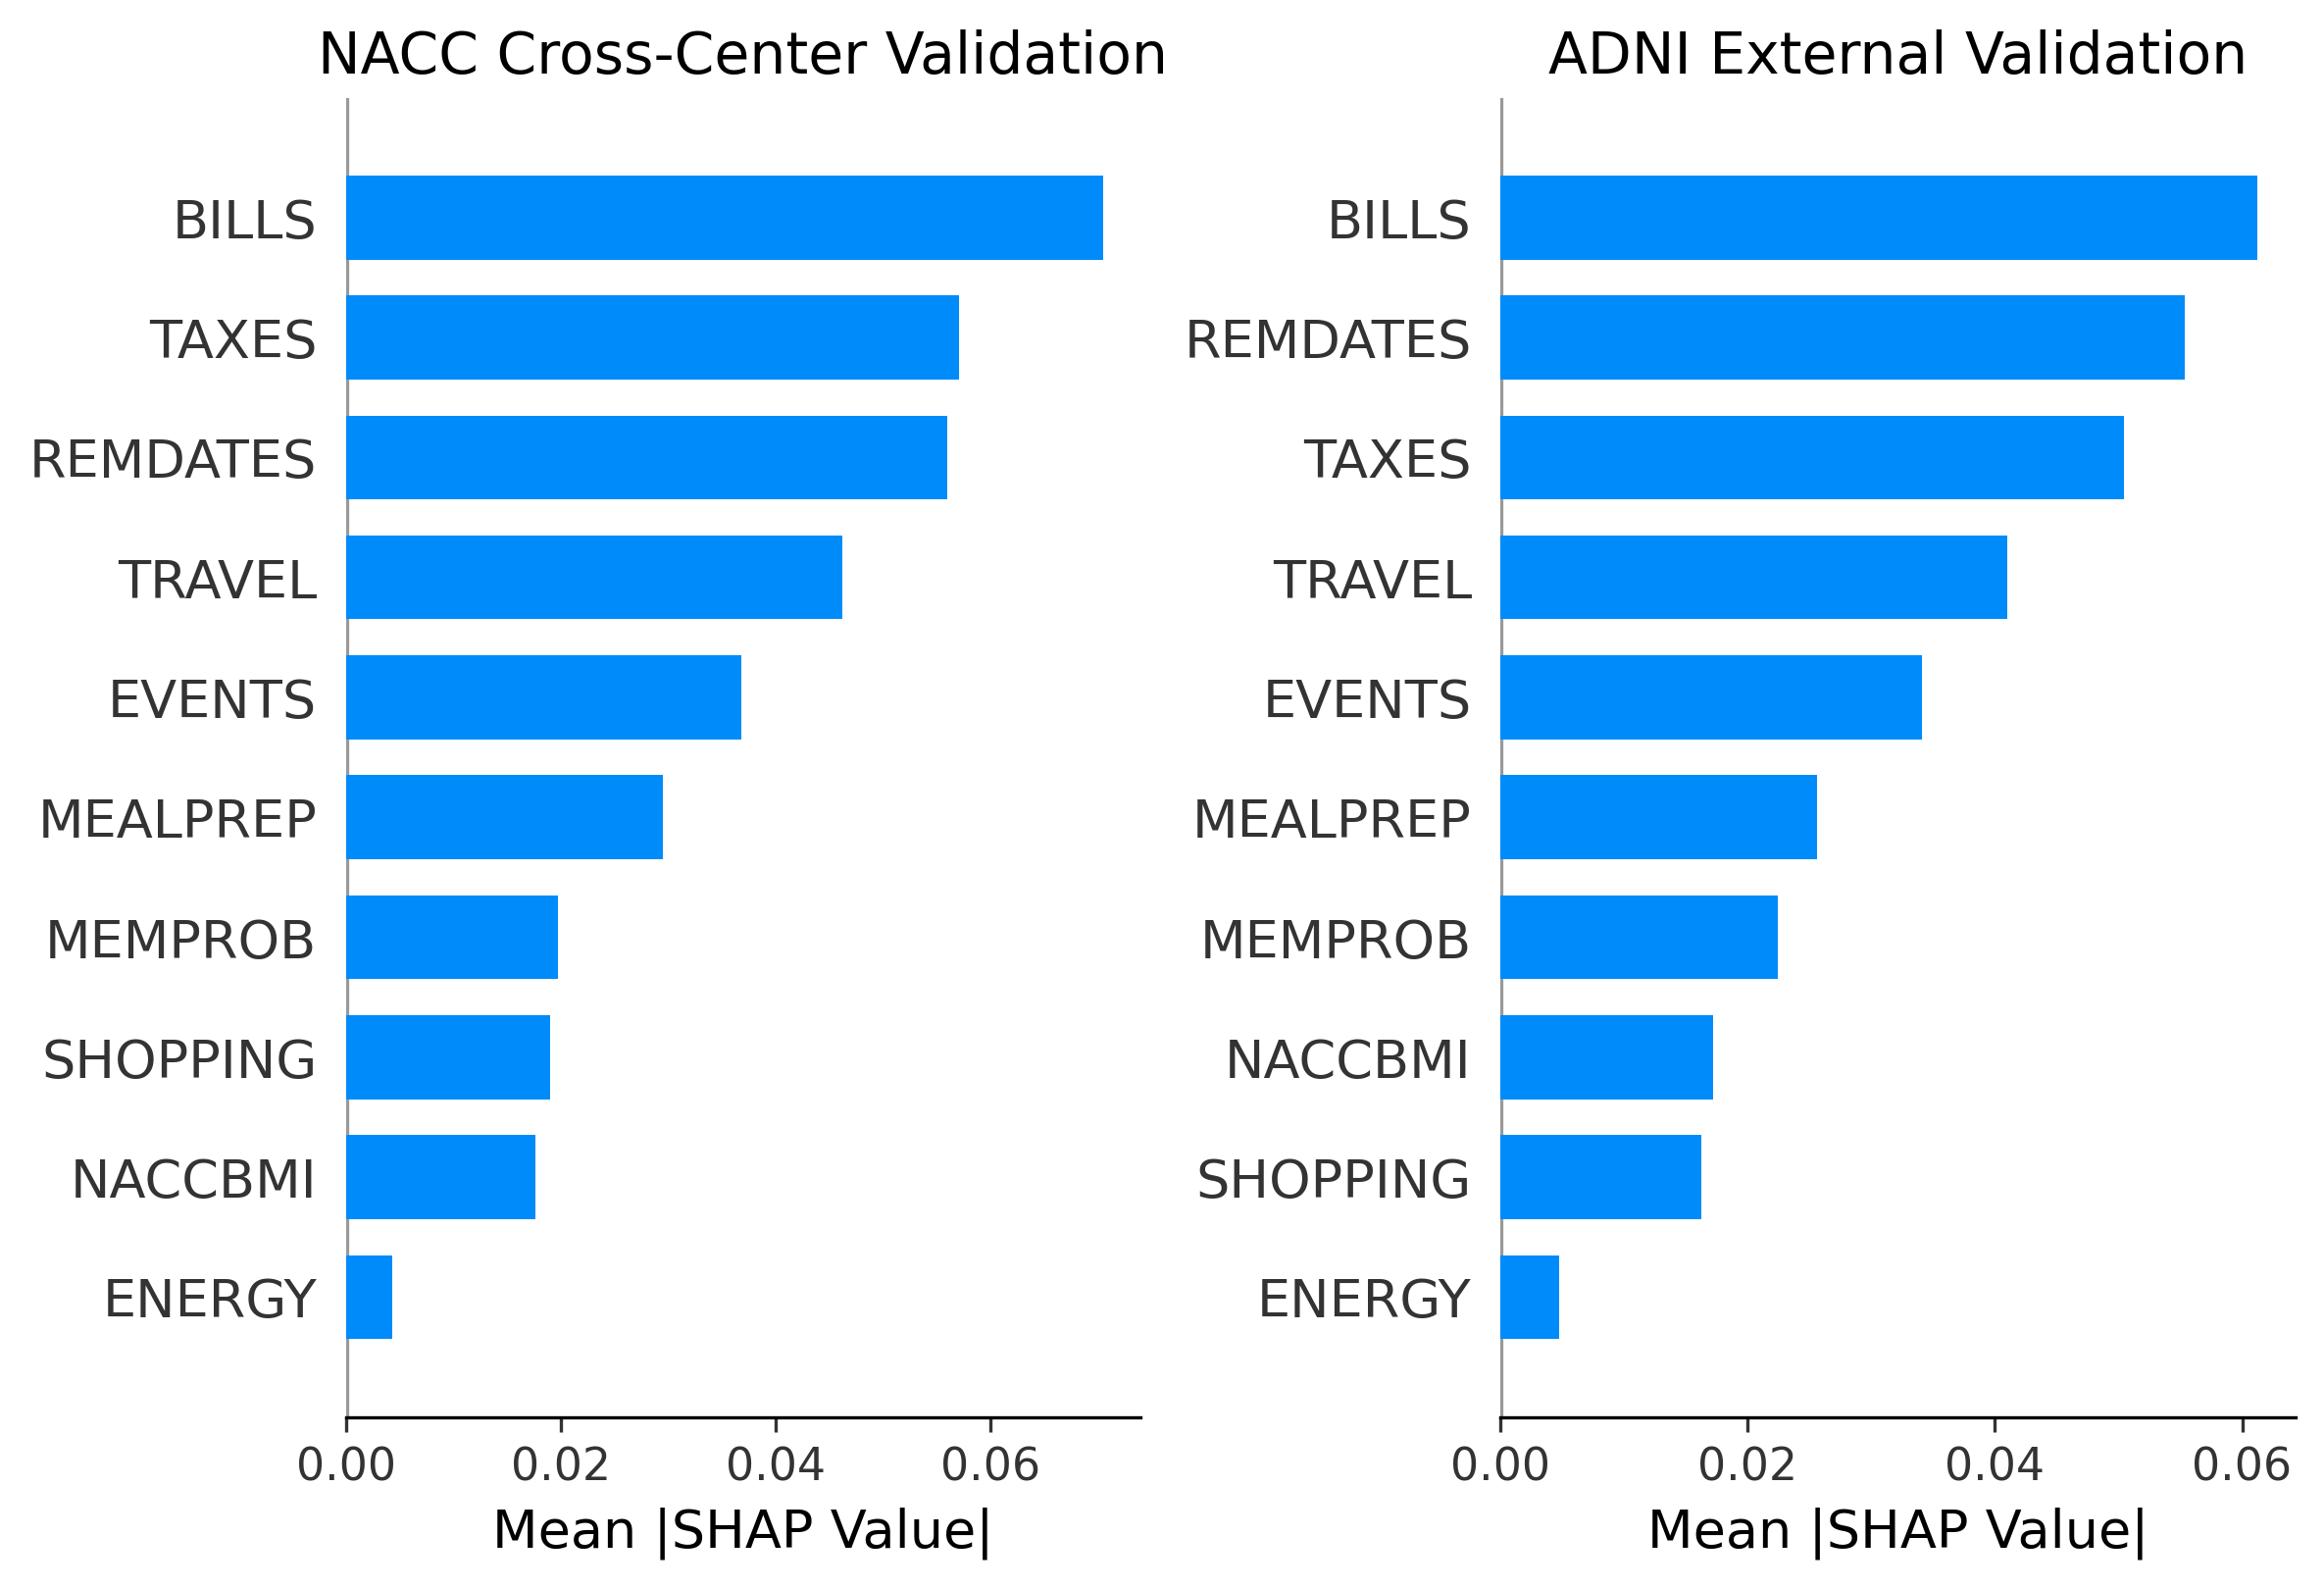
\includegraphics[width=1.0\textwidth]{figures/XAI/dementia_prediction_both_feature_importance_comparison.png}
    \caption{Feature importance in the NACC cross-center validation and the ADNI external validation for the future CIND vs. dementia prediction task}
    \begin{minipage}{\textwidth}
      \footnotesize \hl{The bars represent the mean absolute SHAP value of each feature, which ranks the contribution of the feature to the model prediction in the two validation datasets.}
    \end{minipage}
    \label{figure:cind_dementia_prediction_feature_importance}
\end{figure}

The local explanation of the selected LR model for the future prediction of CIND vs. dementia was assessed. The model was found to be capable of capturing heterogeneous impairment patterns that lead to similar diagnostic outcomes. For the correctly predicted dementia instances in Figure~\ref{figure:cind_dementia_prediction_pos_waterfall}, both \textit{Instance A} and \textit{Instance B} were predicted with similar probabilities of 54\% and 56\%, respectively. Both instances differ in the main risk factor that led to the prediction of dementia. In Instance A, the risk was primarily increased by the difficulty in assembling tax records (TAXES), while the difficulty in paying bills (BILLS) was a major risk factor in Instance B. Despite these differences, both instances shared a common underlying risk driven by memory problems (MEMPROB) and difficulty remembering dates (REMDATES).

\begin{figure}[ht]
    \centering
    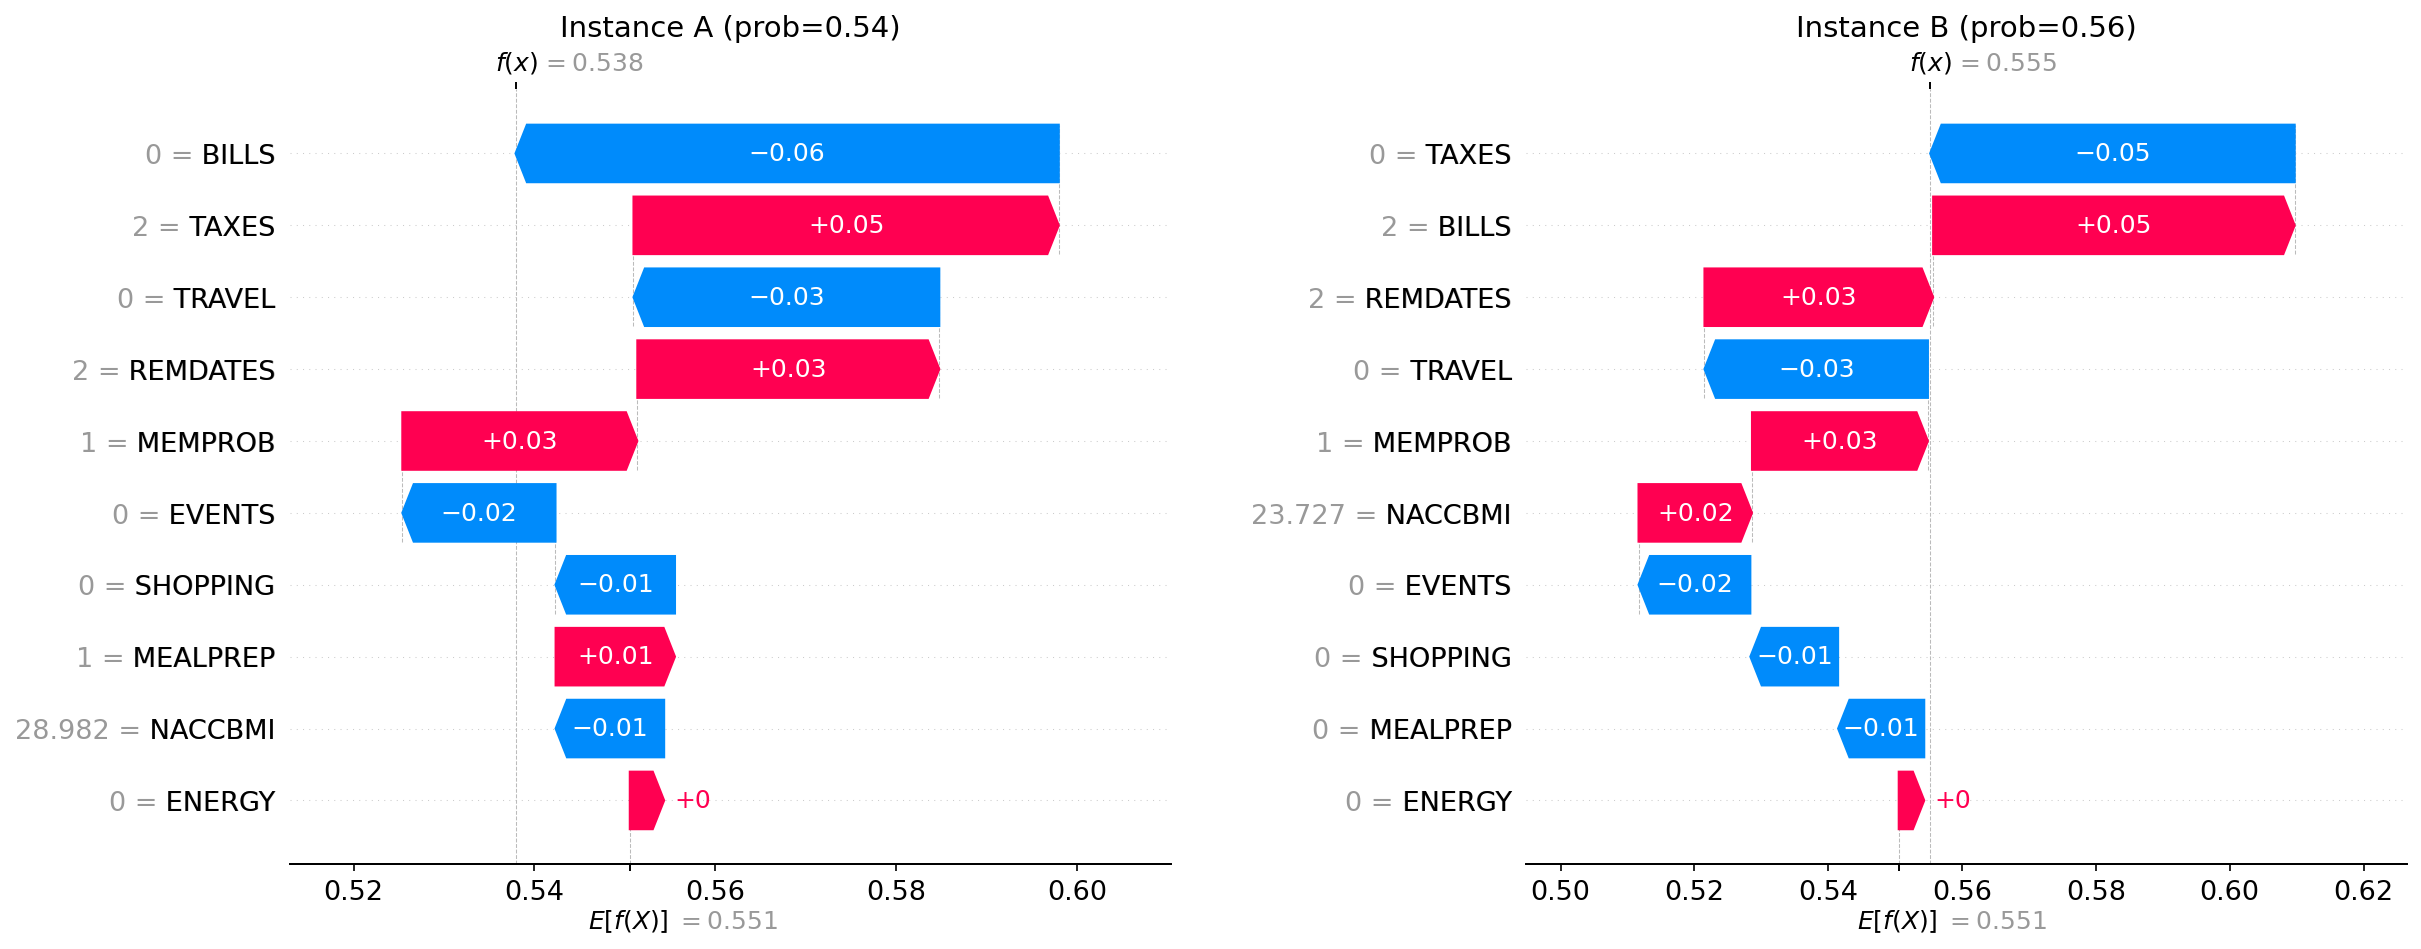
\includegraphics[width=1.0\textwidth]{figures/XAI/dementia_prediction_adni_true_positive_waterfall.png}
    \caption{SHAP waterfall plots for two instances correctly predicted as having risk of dementia within five years in future}
    \begin{minipage}{\textwidth}
      \footnotesize \hl{The plot shows how the value of each feature shifts the prediction from the base value to the final predicted probability for a single instance.}
    \end{minipage}
    \label{figure:cind_dementia_prediction_pos_waterfall}
\end{figure}

\newpage
Figure~\ref{figure:cind_dementia_prediction_neg_waterfall} shows the waterfall plots of two instances correctly predicted as CIND. \textit{Instance B} had a predicted probability of dementia lower than the classification threshold (43\% < 50\%). The low risk of dementia in this case was due to the ability to normally perform critical functional activities (REMDATES, TRAVEL, and EVENTS) and the absence of memory problems. This profile was quite different from Instance A, which had a similar predicted probability (44\%) despite difficulty traveling alone and reported memory problems. This is because executive functions related to financial management (BILLS, TAXES) were preserved as normal in Instance A.

\begin{figure}[ht]
    \centering
    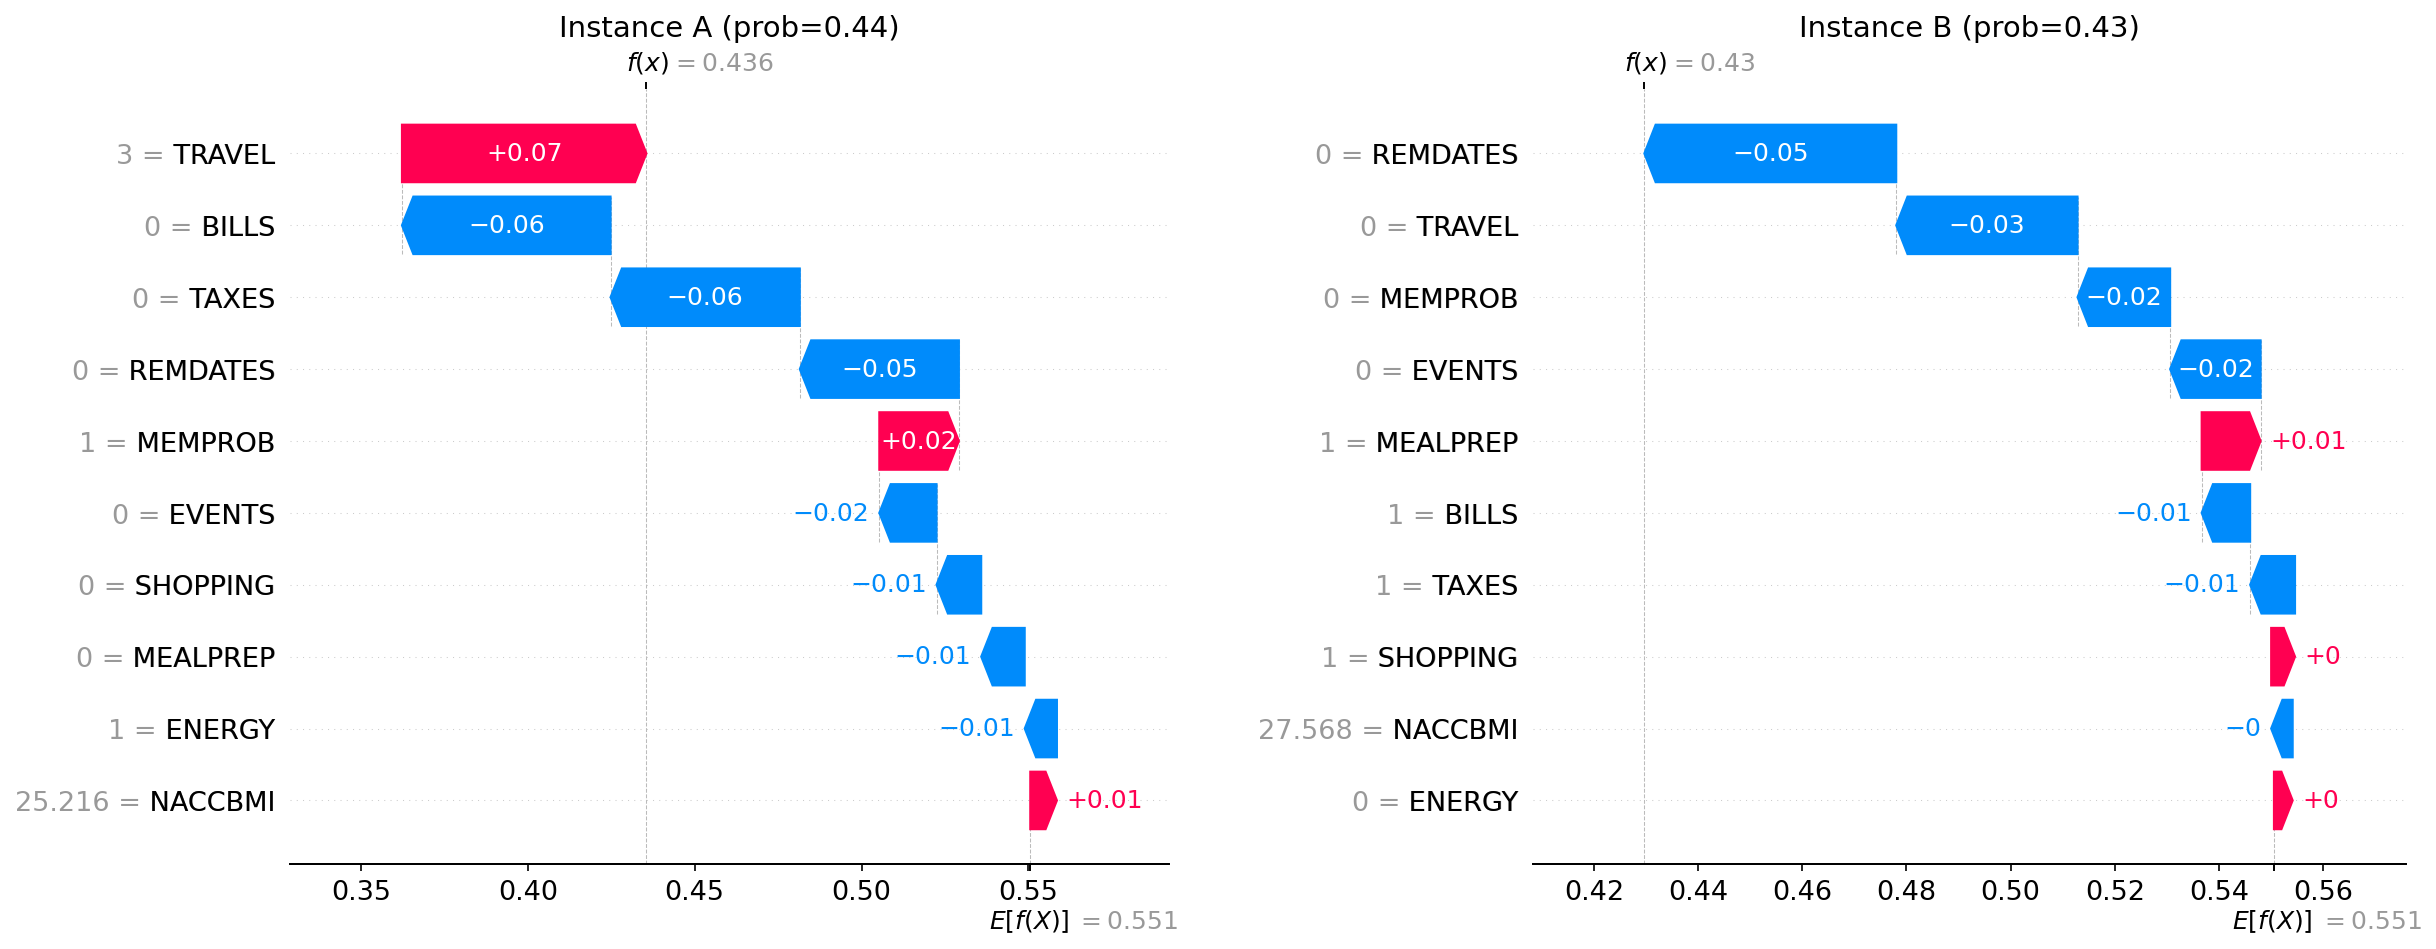
\includegraphics[width=1.0\textwidth]{figures/XAI/dementia_prediction_adni_true_negative_waterfall.png}
    \caption{SHAP waterfall plots for two instances correctly predicted as having risk of CIND within five years in future}
    \begin{minipage}{\textwidth}
      \footnotesize \hl{The plot shows how the value of each feature shifts the prediction from the base value to the final predicted probability for a single instance.}
    \end{minipage}
    \label{figure:cind_dementia_prediction_neg_waterfall}
\end{figure}

\newpage
For counterfactual explanation, using DiCE with the \acrshort{KD-Tree} (K-dimensional tree) search method failed to generate counterfactual examples for half of the ADNI samples. This is because of the limited size and sparsity of the training data in this task, which leaves large gaps between the data points in the KD-Tree structure. As a result, the algorithm was unable to find enough similar instances to construct valid counterfactuals. To overcome this challenge, DiCE with random search was utilized in this task. Random search is not affected by the sparsity of the training data because it generates new synthetic examples by exploring the range of possible feature values to obtain the required outcome.

The DiCE random search method managed to generate counterfactual explanations for risk prevention for only 86.8\% of the ADNI external data instances. This rate is lower than the rates of the other classification and prediction tasks. However, DiCE in this task was able to provide up to five different counterfactual examples for around 72\% of the instances, significantly exceeding the results of the NC vs. CI prediction task. The results of the counterfactual explanation for the future prediction of CIND vs. dementia are presented in Figure~\ref{figure:cind_dementia_prediction_dice_stat}. Analysis of feature changes indicates that the effort required to prevent the risk of dementia is low, with a median of two feature changes. In fact, more than half of the generated counterfactuals (52.8\%) required modifying only one or two risk factors (features). The counterfactual explanation results of the NACC cross-center validation, which are presented in Figure~\ref{figure:dice-nacc-task4-apdx} in the Appendix, showed a similar pattern with a higher percentage of instances without counterfactual examples.

\begin{figure}[ht]
    \centering
    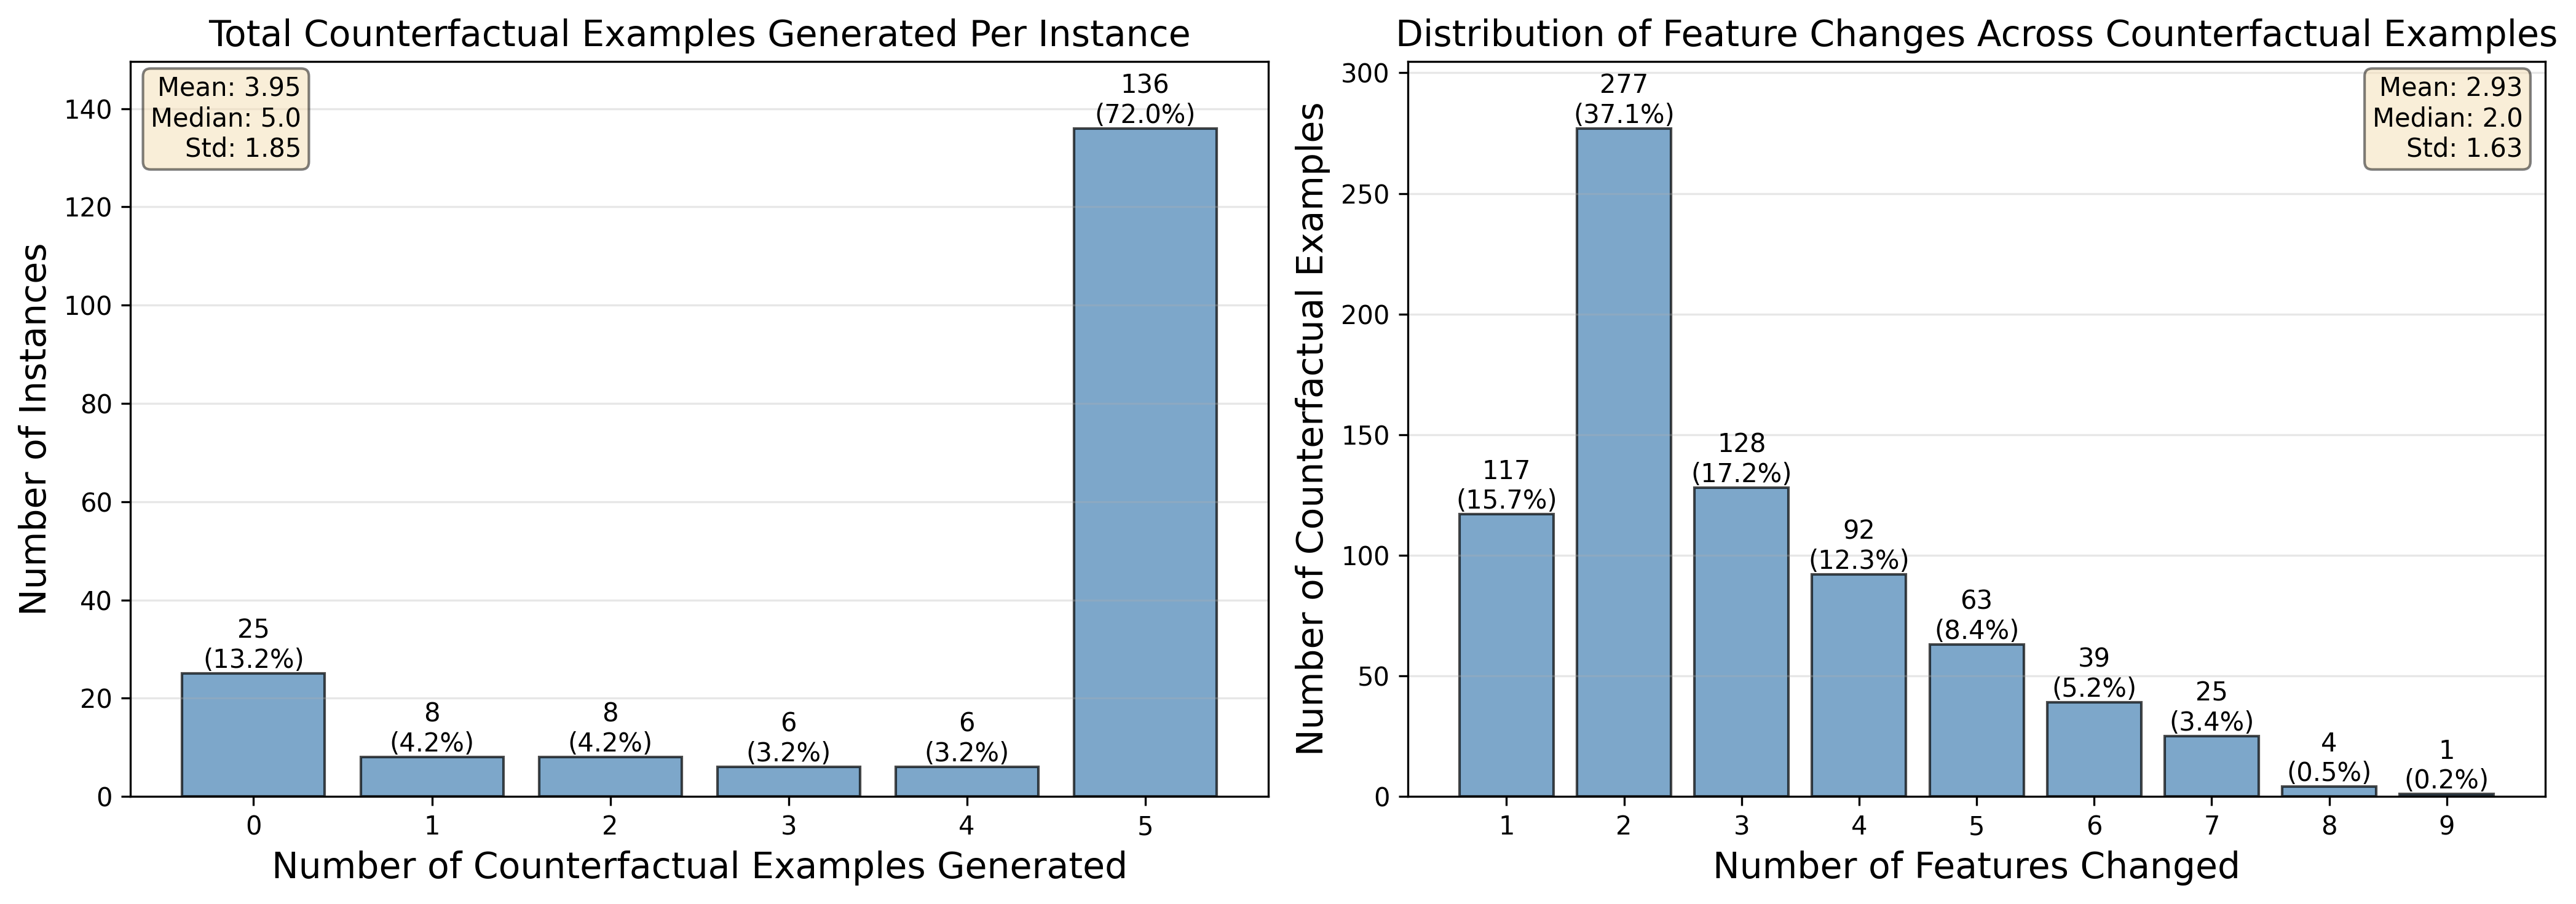
\includegraphics[width=1.0\textwidth]{figures/XAI/dementia_prediction_adni_random_dice_stats.png}
    \caption{Summary of generated counterfactual examples for changing predicted risk from dementia to CIND}
    \label{figure:cind_dementia_prediction_dice_stat}
\end{figure}

The features that should be prioritized for the prevention of the risk of dementia are ranked in Figure~\ref{figure:cind_dementia_prediction_dice_feature_importance}. The ability to remember dates and appointments (REMDATES) was the most frequently modified feature (54\%). Financial management activities from FAQ were also important, with changes in paying bills (BILLS) and  handling taxes (TAXES) contributing to 50\% and 47\% of the generated counterfactual examples, respectively. In contrast, body mass index (NACCBMI), self-reported memory problems (MEMPROB), energy levels (ENERGY) and other functional activities (MEALPREP and SHOPPING) changed in 20\% or fewer of the counterfactual examples generated. Table~\ref{table:cfe-adni-task4-apdx} in the appendix illustrates counterfactual examples generated for a random subject with a future risk of dementia to reverse the estimated outcome to CIND.

\begin{figure}[ht]
    \centering
    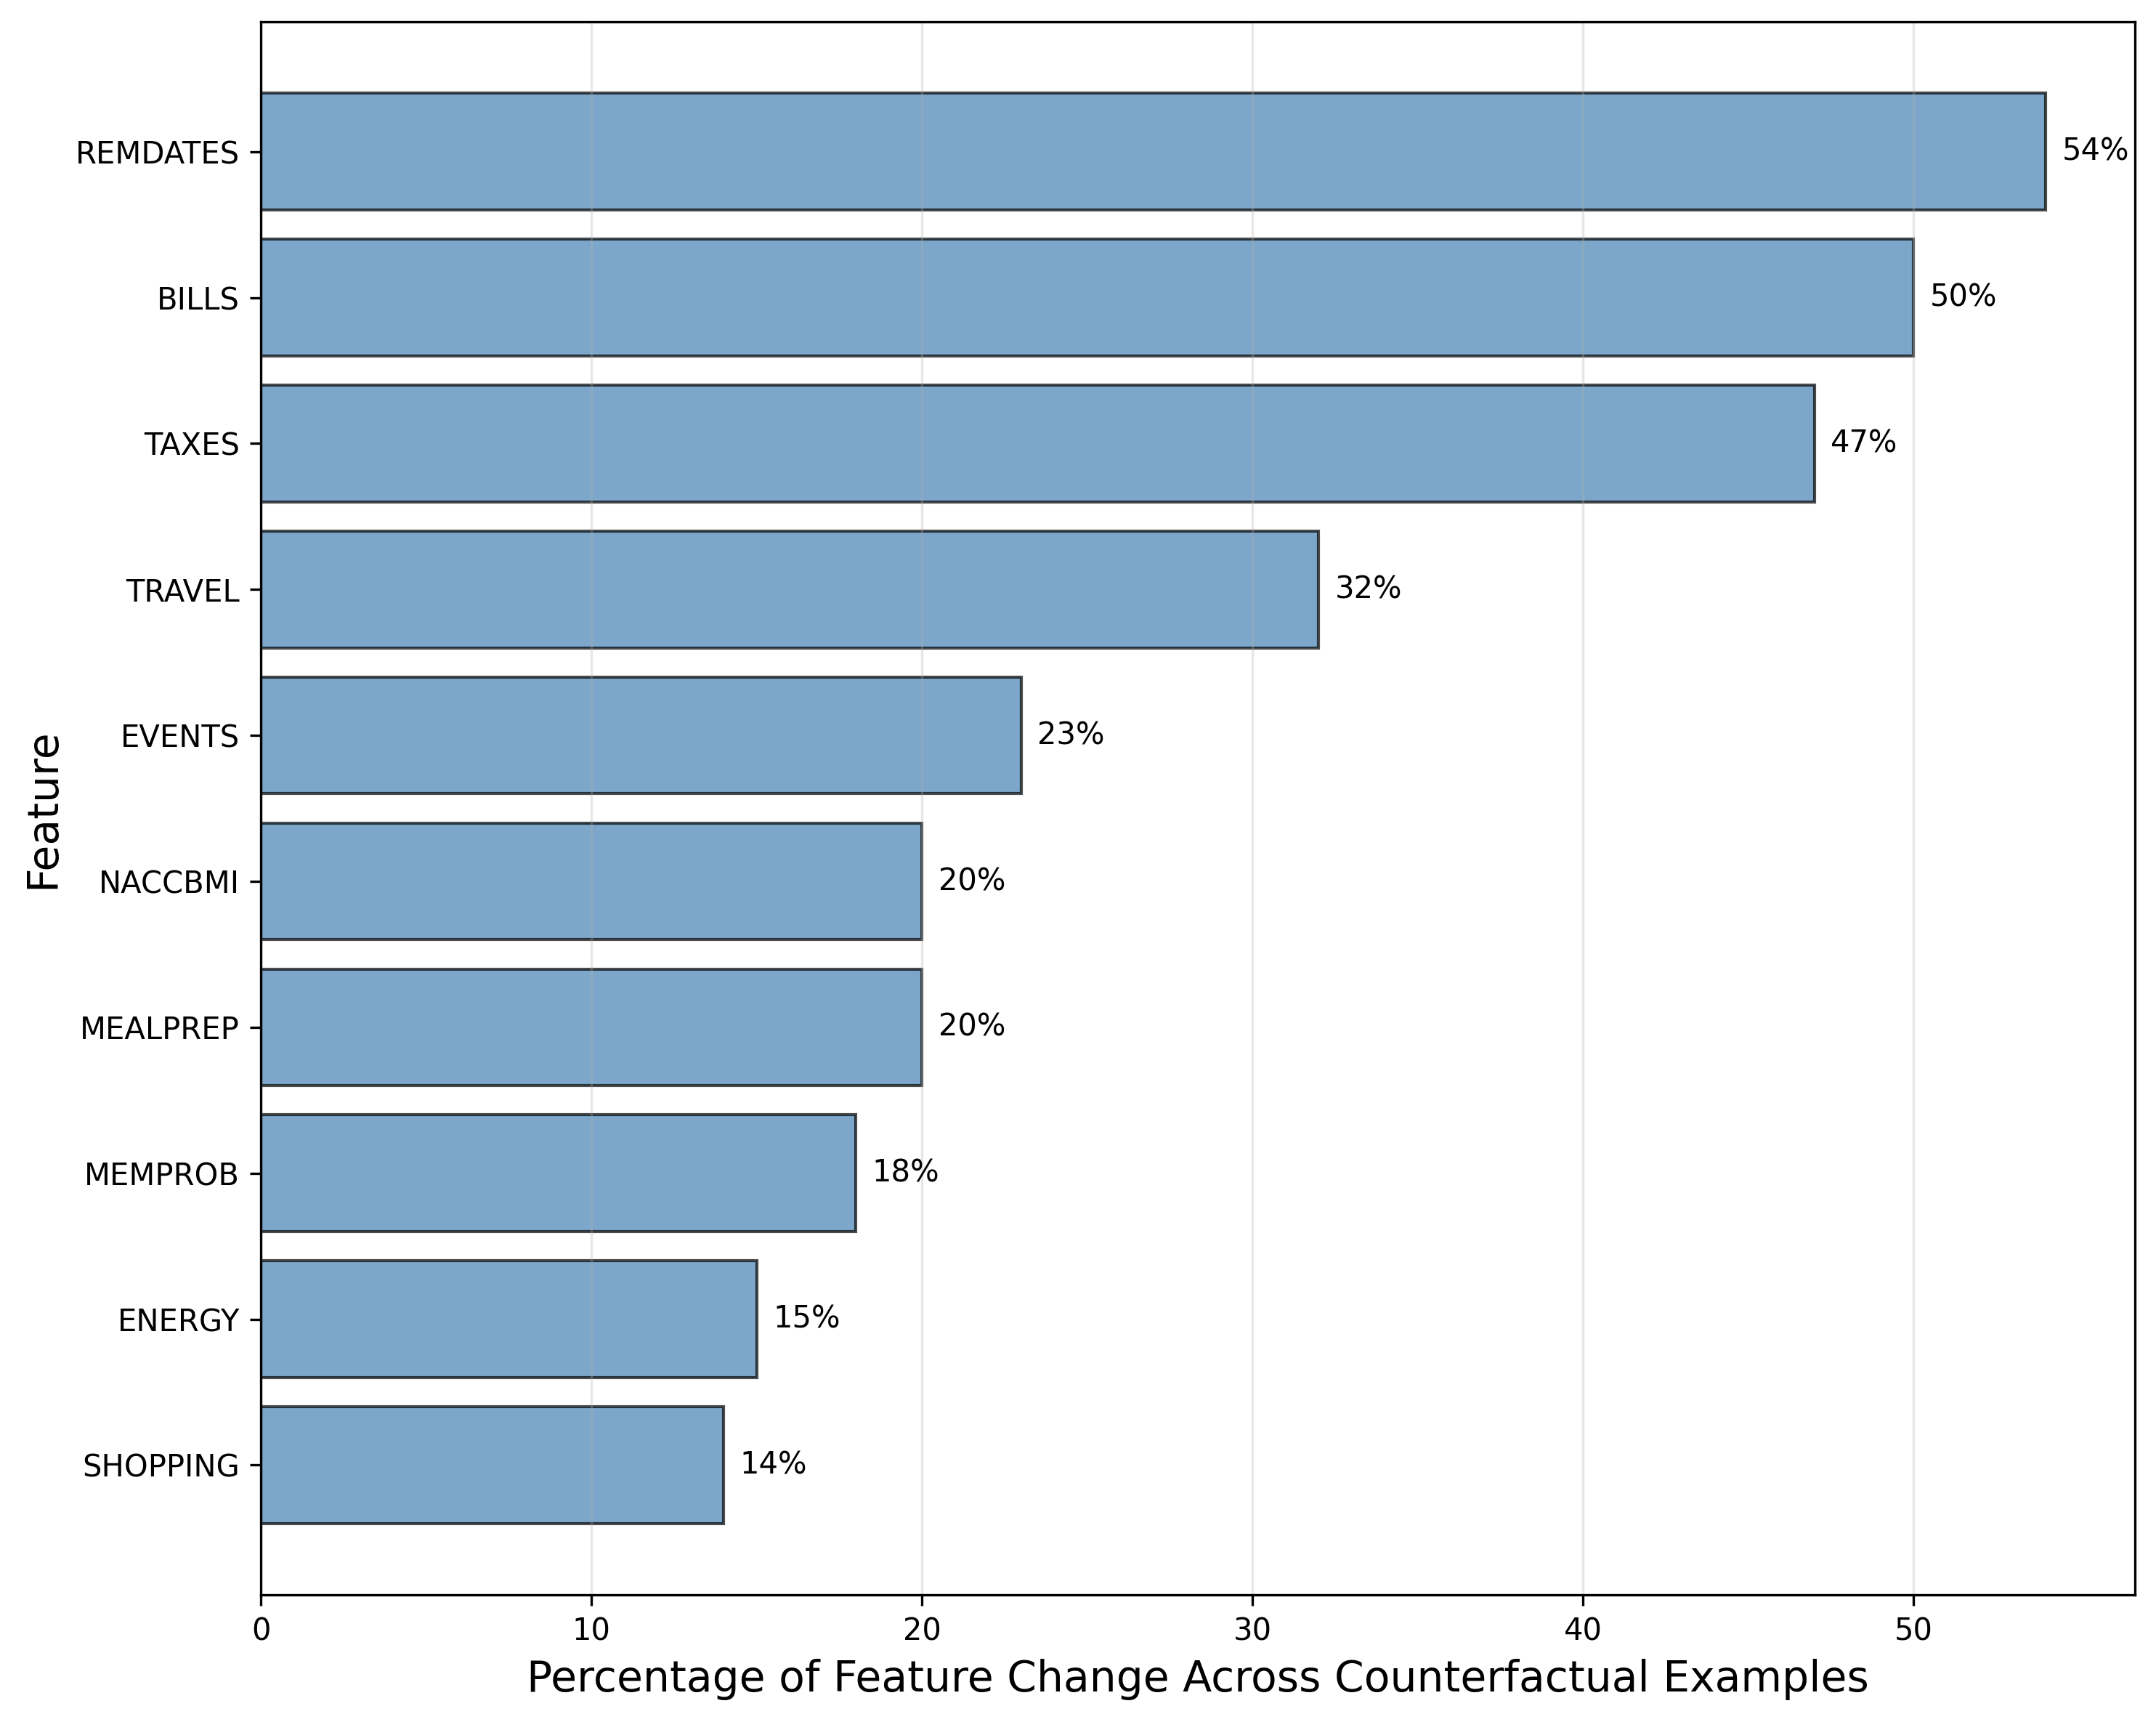
\includegraphics[width=1.0\textwidth]{figures/XAI/dementia_prediction_adni_random_dice_global_importance.png}
    \caption{Feature importance ranking based on counterfactual explanations for the future CIND vs. dementia prediction task}
    \begin{minipage}{\textwidth}
      \footnotesize The features are ranked based on the percentage of times they were modified to generate valid counterfactual examples. The rank highlights the most critical features for risk intervention.
    \end{minipage}
    \label{figure:cind_dementia_prediction_dice_feature_importance}
\end{figure}

\section{Cognitive Impairment Subtype Classification Results}
This section addresses the third research objective: the classification of cognitive impairment subtypes, specifically Alzheimer's Disease (\acrshort{AD}) vs. non-AD etiologies. As hypothesized in the introduction, this task is expected to be the most challenging due to the expected major feature overlap between different types of cognitive impairment.

\subsection{Feature Selection Results}
The evaluation of the feature selection method was applied to this classification task. The proposed method was compared with the baseline and the Boruta method. The results of the comparison using the standard RF model are presented in Table~\ref{table:fs-task5}.

\begin{table}[!ht]
    \centering
    \caption{Comparison of feature selection methods for the AD vs. non-AD classification task}
    \begin{tabular}{|c|c|c|c|c|}
    \hline
        Method & Number of Features & G-mean & Fitness Score & F1 \\ \hline
        Baseline & 77 & 0.730 & 0.608 & 0.988 \\ \hline
        Boruta & 12 & 0.699 & 0.723 & 0.955 \\ \hline
        \textbf{Proposed Method} & \textbf{8} & \textbf{0.668} & \textbf{0.706} & \textbf{0.931} \\ \hline
        \multicolumn{5}{p{400pt}}{\footnotesize \hl{F1: Fisher's discriminant ratio (feature overlap measure), Fitness Score: combined score balancing performance and feature reduction, G-mean: geometric mean score.}}
    \end{tabular}
    \label{table:fs-task5}
\end{table}

The results confirm the high difficulty of this task, with lower G-mean scores in all methods compared to the scores obtained in the cognitive status classification and prediction tasks. The complexity can be noticed from the high F1 class overlap scores. The baseline achieved the highest G-mean (0.730) but the lowest fitness score (0.608) because it used all 77 features. The proposed method was the most successful in reducing complexity and improving efficiency by selecting only eight features. This subset achieved the lowest F1 class overlap score (0.931) and had a model training speed that was 2.5 times faster than the baseline.

\newpage
The Boruta method obtained the highest fitness score of 0.723 by selecting 12 features and producing an RF model with a G-mean of 0.699. This resulted in a higher G-mean score than the proposed method (0.668). Given this finding, a supplementary analysis was carried out to assess the robustness of these feature sets. The performance of the three feature sets was evaluated using two other common classifiers: LR and SVM. The G-mean scores of the three models are presented in Table~\ref{table:fs-task5-more-models}.

\begin{table}[!ht]
    \centering
    \caption{Comparison of feature selection methods in the AD vs. non-AD classification task based on G-mean performance across different models}
    \begin{tabular}{|c|c|c|c|c|}
    \hline
        Method & RF (G-mean) & LR (G-mean) & SVM (G-mean) \\ \hline
        Baseline (77 features) & 0.730 & 0.724 & 0.736 \\ \hline
        Boruta (12 features) & 0.699 & 0.687 & 0.705 \\ \hline
        Proposed Method (8 features) & 0.668 & 0.691 & 0.701 \\ \hline
        \multicolumn{4}{p{400pt}}{\footnotesize \hl{G-mean: geometric mean score, LR: logistic regression, RF: random forest, SVM: support vector machines.}}
    \end{tabular}
    \label{table:fs-task5-more-models}
\end{table}

The G-mean results show that the performance of the selected feature sets is model-dependent. While the baseline performed best overall, the comparison between the proposed method and the Boruta method is more interesting. The 12-feature set from the Boruta method performed best with the RF model, but the 8-feature set from the proposed method achieved a higher G-mean when using the LR model (0.691 vs. 0.687). Both methods were highly comparable when using the SVM model (0.701 vs. 0.705).

The analysis of the feature selection demonstrates that the proposed method is capable of selecting the smallest set of features that could reduce the complexity of the data and increase the computational efficiency of the model. Moreover, the selected features are highly robust and generalizable across different types of classification algorithms.

The eight features that were selected by the proposed method for this CI subtype classification task are listed in Table~\ref{table:features-task5}. 6 out of the 8 features are related to the Clinical Dementia Rating (\acrshort{CDR}) scale. The list also includes the subject's age and a single feature from the FAQ. More details of the selected features and their correlation results can be found in section \ref{sec:feature-selection-apdx} in the appendix.

\begin{table}[h!]
\centering
\caption{List of selected features for the AD vs. non-AD classification task}
\label{table:features-task5}
\begin{tabular}{ccc}
\toprule
\textbf{Feature Code} & \textbf{Feature Description} & \textbf{Feature Category} \\
\midrule
NACCAGE & Age & Demographics \\
MEMORY & Memory & CDR \\
ORIENT & Orientation & CDR \\
JUDGMENT & Judgment \& Problem Solving & CDR \\
COMMUN & Community Affairs & CDR \\
HOMEHOBB & Home \& Hobbies & CDR \\
PERSCARE & Personal Care & CDR \\
REMDATES & Remember dates and appointments & FAQ \\
\bottomrule
\end{tabular}
\end{table}

\subsection{Data Resampling Results}
\label{sec:resampling_results_ro3}
The results of the data resampling method of the AD vs. non-AD classification task are presented in this section. Differentiating AD from non-AD disorders using accessible data was hypothesized to be a challenging task. The complexity of the training data could confirm this. According to the analysis of the class imbalance and overlap, this task presented the most severe data complexity of all tasks in this study. The AD examples are 1.35 more than the minority non-AD examples. Additionally, a very high class overlap was observed with 0.323 instance-level class overlap (kDN) and 0.511 structural class overlap (N1). The analysis of borderline example measures also showed that the minority non-AD class was deeply embedded in the overlapped region, with 46\% of its examples identified as borderline, compared to 34\% for the majority class (AD). The distribution of the target classes in the NACC UDS is presented in Figure~\ref{fig:nacc-data-stat} in the appendix.

This combination of high overlap and a higher proportion of borderline minority examples led to the selection of the ENN + KMeansSMOTE method, as specified by the decision algorithm (Algorithm \ref{alg:data-resampling}). ENN was first applied to clean overlapped instances, and then KMeansSMOTE was used to increase the minority class occurrence in safe clusters instead of adding more minority examples around the already complex decision boundary. The performance of this selected strategy was then assessed against the baseline and standard resampling methods. Table~\ref{table:ad_nonad_resampling} lists the results of this comparison. The results are also illustrated in Figure~\ref{figure:ad_nonad_resampling_perf}.

As shown in Table~\ref{table:ad_nonad_resampling}, the severe overlap in the baseline data resulted in a low balanced performance (G-mean = 0.668). This is because the RF model was unable to accurately classify the minority non-AD class (recall = 0.626). It is important to note that oversampling methods like ROS and SMOTE were ineffective as they failed to reduce the class overlap. Although these methods resulted in an improvement in non-AD recall, they lead to a considerable decrease in AD recall from 0.714 to 0.666 in ROS and 0.677 in SMOTE. This dramatic change in the performance of the RF model in both classes was also observed in the RUS method, where the non-AD recall increased to the highest score of  0.712 while the AD recall dropped by 7.5 percentage points to the lowest score of 0.639. The application of the RUS method resulted in an increase in the structural class overlap (N1) to 0.522. 

\begin{table}[!ht]
    \centering
    \caption{Performance comparison of resampling methods for the AD vs. non-AD classification task using a random forest model}
    \begin{tabular}{|c|c|c|c|c|c|}
    \hline
        Method & G-mean & Recall (AD) & Recall (non-AD) & kDN & N1 \\ \hline
        Baseline & 0.668 & 0.714 & 0.626 & 0.323 & 0.511 \\ \hline
        ROS & \makecell{0.673 \\ {\small \hl{(p = 0.125)}}} & 0.666 & 0.681 & 0.317 & 0.503 \\ \hline
        RUS & \makecell{0.674 \\ {\small \hl{(p = 0.157)}}} & 0.639 & \textbf{0.712} & 0.306 & 0.522 \\ \hline
        SMOTE & \makecell{0.674 \\ {\small \hl{(p = 0.011)}}} & 0.677 & 0.671 & 0.315 & 0.491 \\ \hline
        \makecell{\textbf{ENN +} \\ \textbf{KMeansSMOTE}} & \makecell{\textbf{0.710} \\ {\small \hl{(p = 0.001)}}} & \textbf{0.729} & 0.692 & \textbf{0.021} & \textbf{0.125} \\ \hline
        \multicolumn{6}{p{400pt}}{\footnotesize \hl{G-mean: geometric mean score, kDN: k-disagreeing neighbors (instance-level class overlap), N1: structural class overlap, Recall: per-class recall.}}
    \end{tabular}
    \label{table:ad_nonad_resampling}
\end{table}

\begin{figure}[ht]
\centering
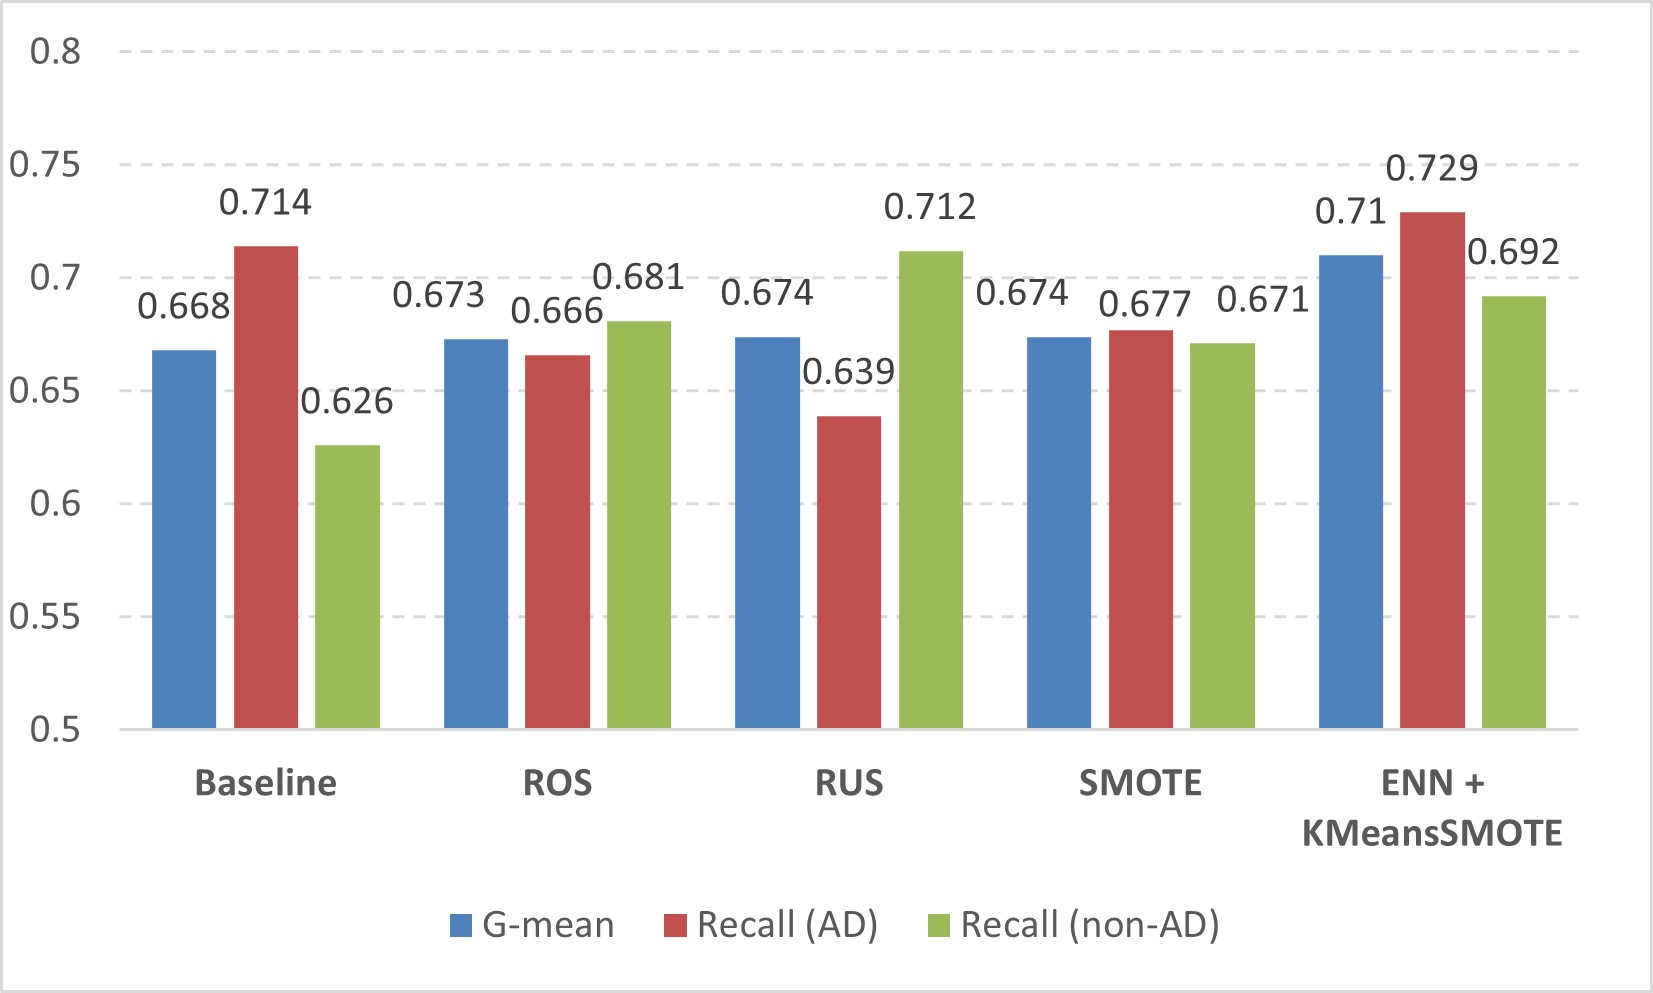
\includegraphics[width=1\textwidth]{figures/data-resampling-task5.jpg}
\caption{Model performance comparison of data resampling methods for the AD vs. non-AD classification task}
\label{figure:ad_nonad_resampling_perf}
\end{figure}

In contrast, the selected ENN + KMeansSMOTE method produced the most effective and balanced RF model. It was the only method that successfully addressed the data complexity by totally reducing both instance-level and structural class overlap. As a result, this method achieved the highest G-mean of 0.710. This is more than 4 percentage points of improvement from the baseline model. It did this by significantly improving the recall of the minority non-AD class to 0.692 while achieving the highest recall for the AD class at 0.729. This confirms that for this highly complex task, a specialized strategy that first cleans the overlap and then systematically resamples the minority class is necessary to achieve a balanced and effective classification model. \hl{The G-mean improvement of the proposed ENN + KMeansSMOTE method over the baseline was highly significant (p = 0.001) and was the strongest result among all the evaluated methods, which confirms the effectiveness of the proposed strategy in this complex task.}

\subsection{Model Fine-tuning and Selection Results}
The final model fine-tuning and selection process was also applied to the CI subtype classification task. The results of optimizing and selecting the best model that distinguishes between AD and non-AD disorders are outlined in this section.

The cost-effective selection algorithm (Algorithm \ref{alg:model-selection}) was again utilized to identify the most suitable models. The G-mean metric was used to evaluate the performance of the models with a balanced evaluation of both classes. The selection algorithm successfully identified sets of hyperparameters that offered significant speed improvements for most models. The training speed of the LR and KNN models improved by around 1.3 times while maintaining the same G-mean scores as the best-performing models. The highest gain in prediction speed was achieved by the KNN model (2.39 times), followed by the LightGBM model (1.49 times) and the LR model (1.2 times). The performance and throughput of the five optimized models are presented in Table~\ref{table:task5_finalists_models}.

\begin{table}[!ht]
\centering
\caption{Summary of fine-tuned models for the AD vs. non-AD Classification Task}
\label{table:task5_finalists_models}
\newcolumntype{C}{>{\centering\arraybackslash}X}
    \begin{tabularx}{\textwidth}{|C|C|C|C|}
        \hline
        \textbf{Model} &
        \textbf{G-mean\newline(95\% CI)} &
        \textbf{Training Throughput (Gain)\textsuperscript{1}} &
        \textbf{Prediction Throughput (Gain)\textsuperscript{1}} \\
        \hline
        KNN &
        0.682 ($\pm 0.006$) &
        $778,285$ $(1.31\times)$ &
        $47,963$ $(2.39\times)$ \\
        \hline
        LR &
        0.702 ($\pm 0.005$) &
        $1,123,435$ $(1.34\times)$ &
        $19,910,963$ $(1.20\times)$ \\
        \hline
        LightGBM &
        0.699 ($\pm 0.005$) &
        $192,613$ $(1.03\times)$ &
        $1,086,848$ $(1.49\times)$ \\
        \hline
        RF &
        0.705 ($\pm 0.005$) &
        $29,743$ $(1.04\times)$ &
        $157,279$ $(1.04\times)$ \\
        \hline
        SVM &
        0.709 ($\pm 0.006$) &
        $1,157$ &
        $7,466$ \\
        \hline
        \multicolumn{4}{p{400pt}}{\footnotesize \textsuperscript{1}\hl{Training throughput is reported in training samples per second, and prediction throughput in predictions per second.} Gain is calculated as the ratio of the selected model’s throughput to the benchmark model’s throughput. Values indicate the factor by which training and prediction speed have improved. Gain is not presented when the selected model is the benchmark model.}
    \end{tabularx}
\end{table}

A final assessment was conducted to select only one best model. Performance, efficiency, and interpretability were the focus of this assessment. The LR model was selected as the best model for its ability to provide a cost-effective classification. Regarding performance, the LR model's G-mean of 0.702 is statistically comparable to the highest-performing SVM (0.709) and RF (0.705) models. Second, on top of high performance, the LR model is also extremely efficient. This efficiency significantly exceeded all models. Even though the SVM model had the highest G-mean, it was the slowest model overall. Finally, the linear nature of the LR model ensures high interpretability, which is a core objective for this study. In contrast, the SVM and RF models are significantly more computationally intensive. In addition, they are more complex to explain. Therefore, the best trade-off of accuracy, high speed, and easy interpretability is offered by the LR model. Table~\ref{table:lr-fine-tune-task5-apdx} in the appendix presents the hyperparameter fine-tuning results of the LR model.

In summary, the model fine-tuning and selection process has been successfully completed for all five classification tasks. The findings consistently show that the LR models are the most cost-effective across all tasks. By achieving performance that is statistically comparable to more complex models, such as RF and SVM, while offering substantial advantages in computational speed and high interpretability, the LR model successfully addresses the core research objectives concerning cost-effectiveness and explainability. The following sections analyze the external validation and model explainability of the selected LR models.

\subsection{Model Performance in External Validation}
The generalizability of the selected LR model for the AD vs. non-AD classification task was tested on the holdout NACC cross-center testing dataset, which contains unseen data from different research centers. The details of the validation method are provided in section \ref{sec:model-validation}.

The performance of the model in the NACC cross-center validation was analyzed and compared to the model's performance in the internal CV. The results are listed in Table~\ref{tab:ad_nonad_results}. Additionally, the ROC curves for the internal CV and the NACC cross-center validation are illustrated by Figure~\ref{fig:ad_nonad_roc}.

\begin{table}[!ht]
    \centering
    \caption{Performance of the selected logistic regression model in internal and external validation for the AD vs. non-AD classification task}
    \label{tab:ad_nonad_results}
    \begin{tabular}{|c|c|c|}
        \hline
        \textbf{Metric} & \textbf{Internal CV} & \textbf{NACC Cross-center Validation} \\
        \hline
        AUC & \makecell{0.702 \\ {\small \hl{(0.698--0.706)}}} & \makecell{0.670 \\ {\small \hl{(0.658--0.681)}}} \\ \hline
        G-mean & 0.702 & 0.670 \\ \hline
        Sensitivity & 0.689 & 0.679 \\ \hline
        Specificity & 0.714 & 0.660 \\ \hline
        F1-score & 0.725 & 0.706 \\
        \hline
        \multicolumn{3}{p{400pt}}{\footnotesize \hl{AUC: area under the curve, F1-score: harmonic mean of precision and recall, G-mean: geometric mean score, Sensitivity: recall of the AD class, Specificity: recall of the non-AD class.}}
    \end{tabular}
\end{table}

\begin{figure}[ht]
    \centering
    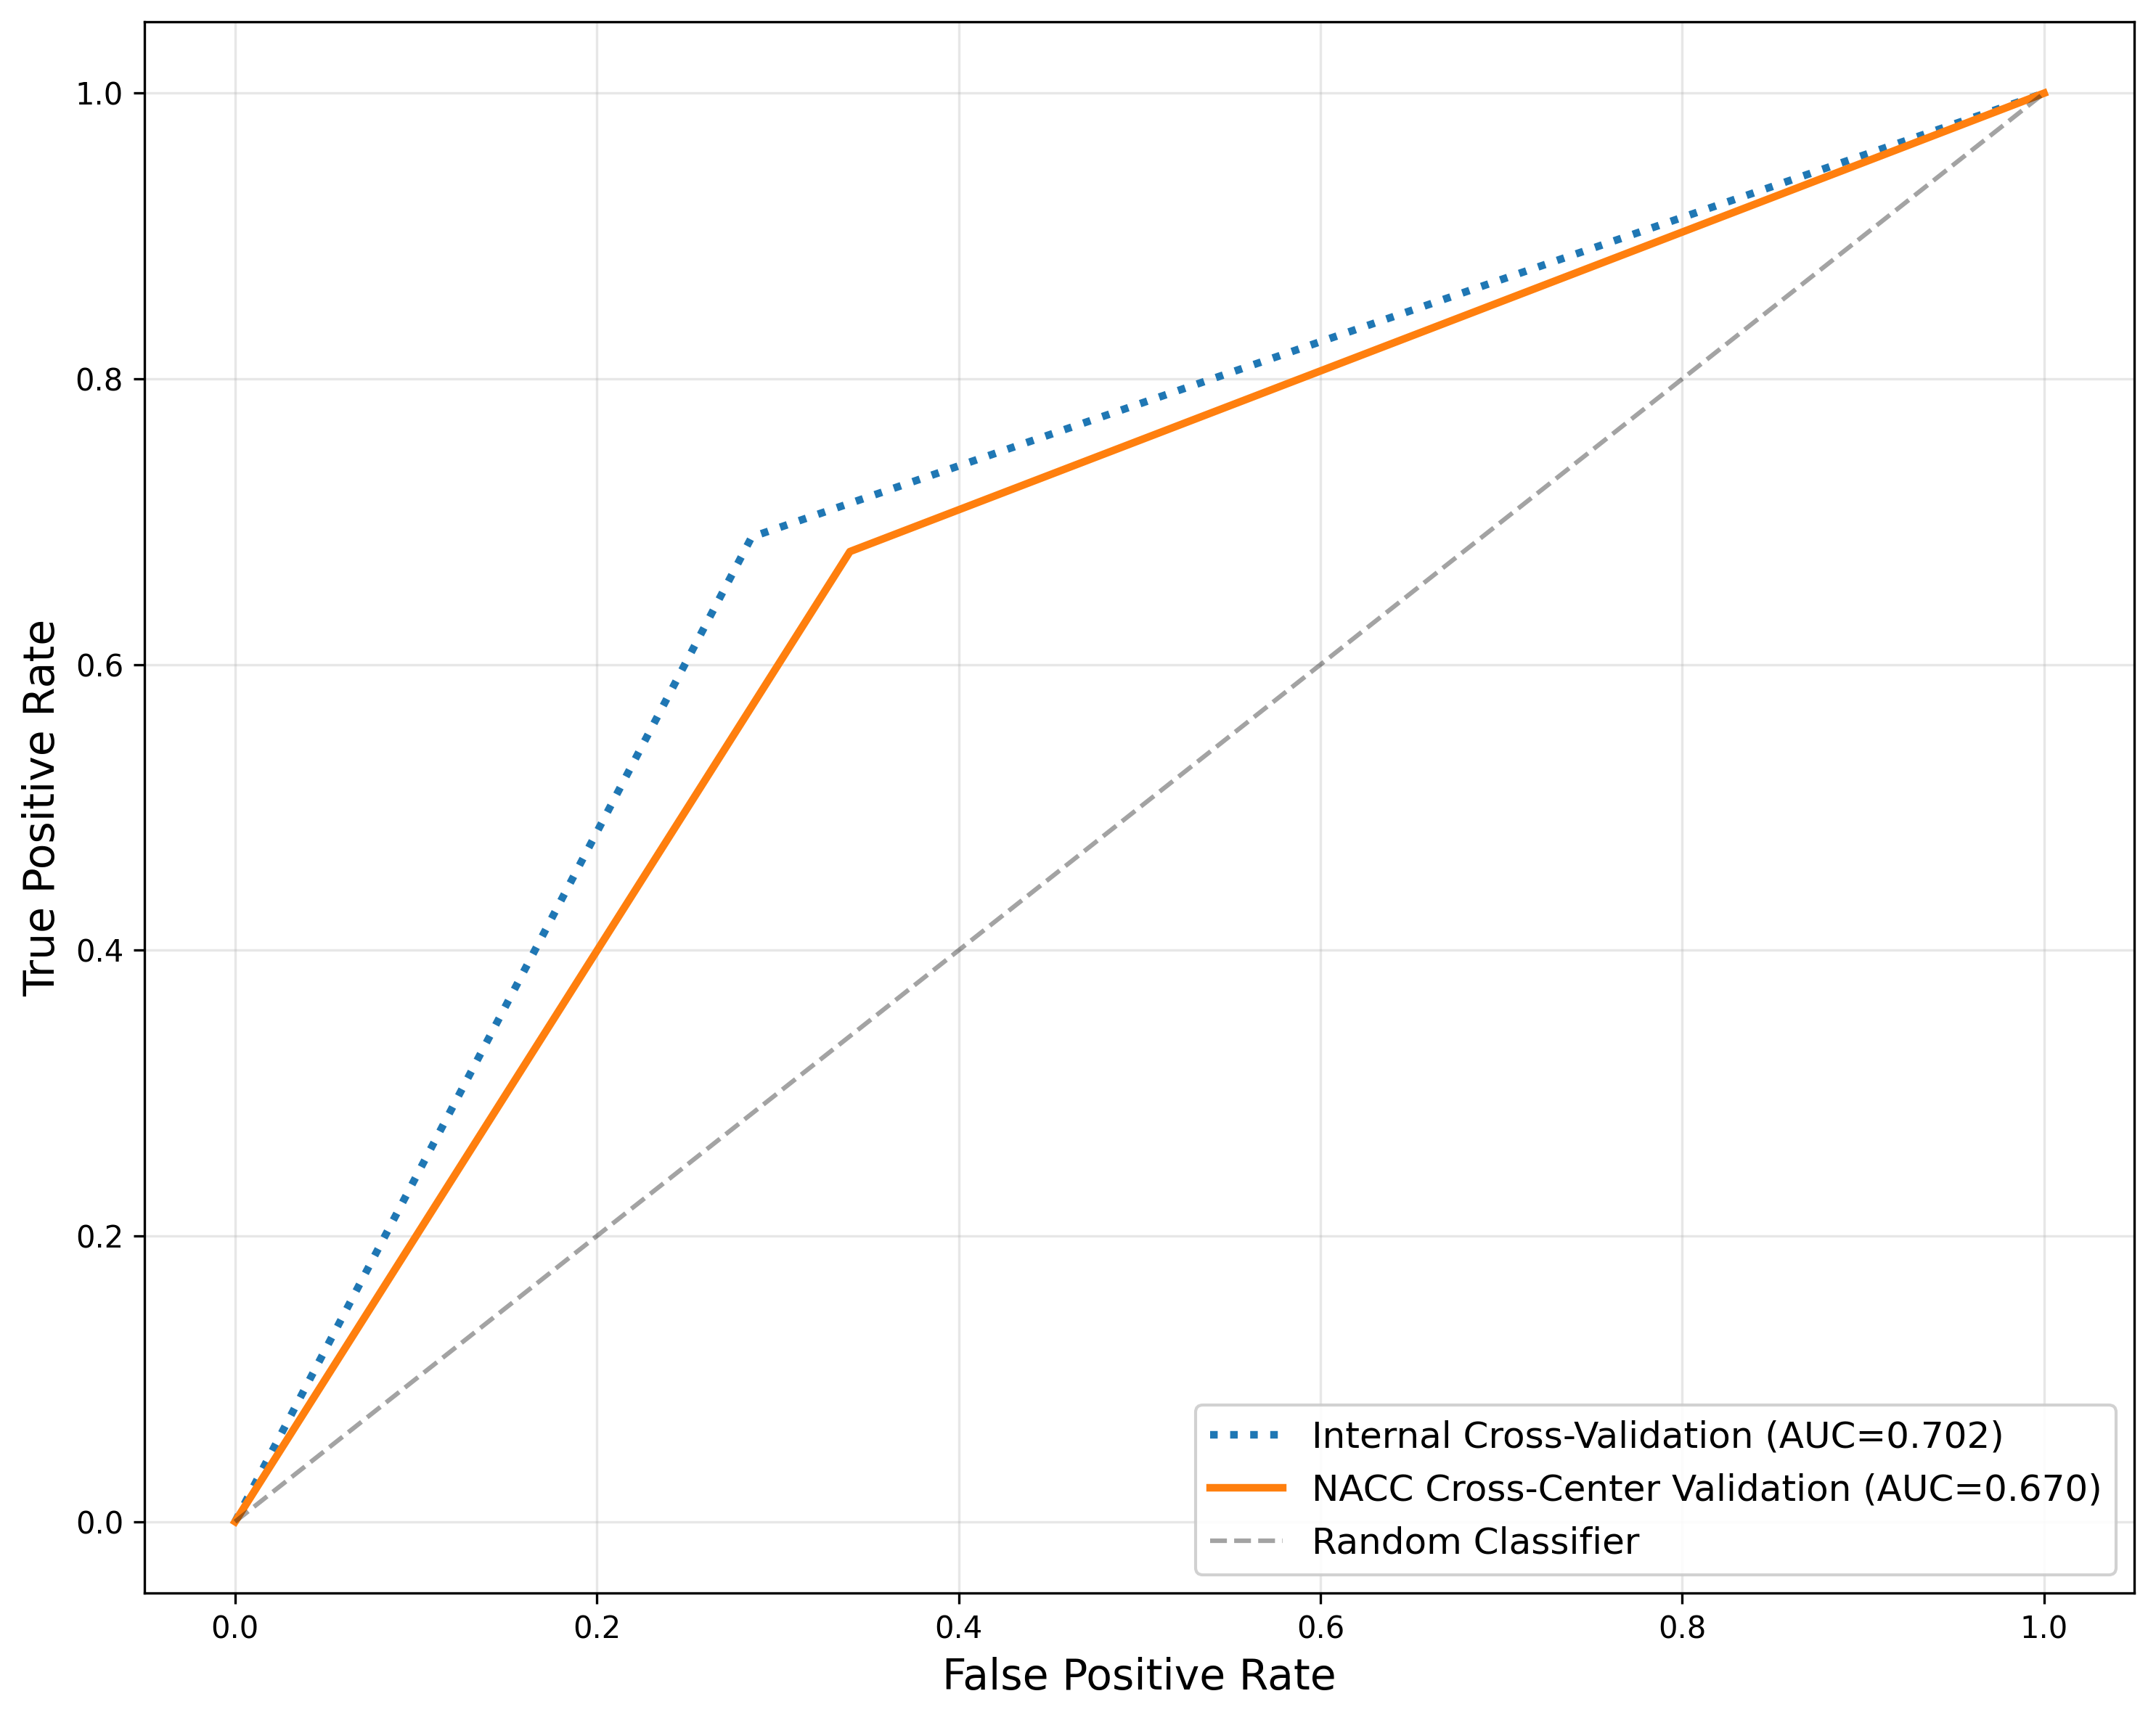
\includegraphics[width=0.7\textwidth]{figures/type_classification_all_tests_roc_overlay.png}
    \caption{ROC curves comparing the performance of the logistic regression model for the AD vs. non-AD classification task}
    \begin{minipage}{\textwidth}
      \footnotesize \hl{The horizontal axis shows the false positive rate (1 -- specificity) and the vertical axis shows the true positive rate (sensitivity). Each curve represents one validation dataset.}
    \end{minipage}
    \label{fig:ad_nonad_roc}
\end{figure}

Based on the results of the NACC cross-center validation, a moderate decrease in overall performance was observed. The AUC score decreased by 0.032, dropping from 0.702 in the internal CV to 0.670 in the NACC cross-center validation. A similar decrease was shown by the G-mean. \hl{This drop in AUC from the internal CV was statistically significant (p < 0.001), although the difference in performance is acceptable for this complex classification task.} This performance reduction confirms the high difficulty of this classification task due to the overlap in symptoms between different CI subtypes.

A slight decrease was observed in both the sensitivity and specificity scores in the unseen NACC data. The sensitivity decreased from 0.689 in the internal CV to 0.679, while the specificity decreased from 0.714 to 0.660. This indicates that the LR model found it more difficult to correctly identify cases in the NACC cross-center validation. The larger reduction in specificity means that more subjects who did not have AD were misclassified as AD. The external validation results are reported with extended performance metrics in Table~\ref{table:lr-complete-perf-task5-apdx} in the appendix.

The selected LR model was calibrated to ensure that the predicted probabilities reflect the actual risk of AD. The calibration results for NACC cross-center validation are shown in Figure~\ref{fig:ad_nonad_calib_curve}. The probabilities of the uncalibrated model were very confident in estimating extreme risk levels (slope = 0.294). However, after beta calibration was applied, the slope improved to 0.859, indicating that the model can now effectively predict AD at different probabilities thresholds. As a result, the model calibration error (ECE) decreased substantially from 0.182 to 0.042, and the Brier score improved from 0.240 to an acceptable level of 0.204, which is close to the acceptable threshold of 0.20. This highlights significant improvements in the overall alignment between the predictions and the actual observed frequencies of AD.

\begin{figure}[ht]
    \centering
    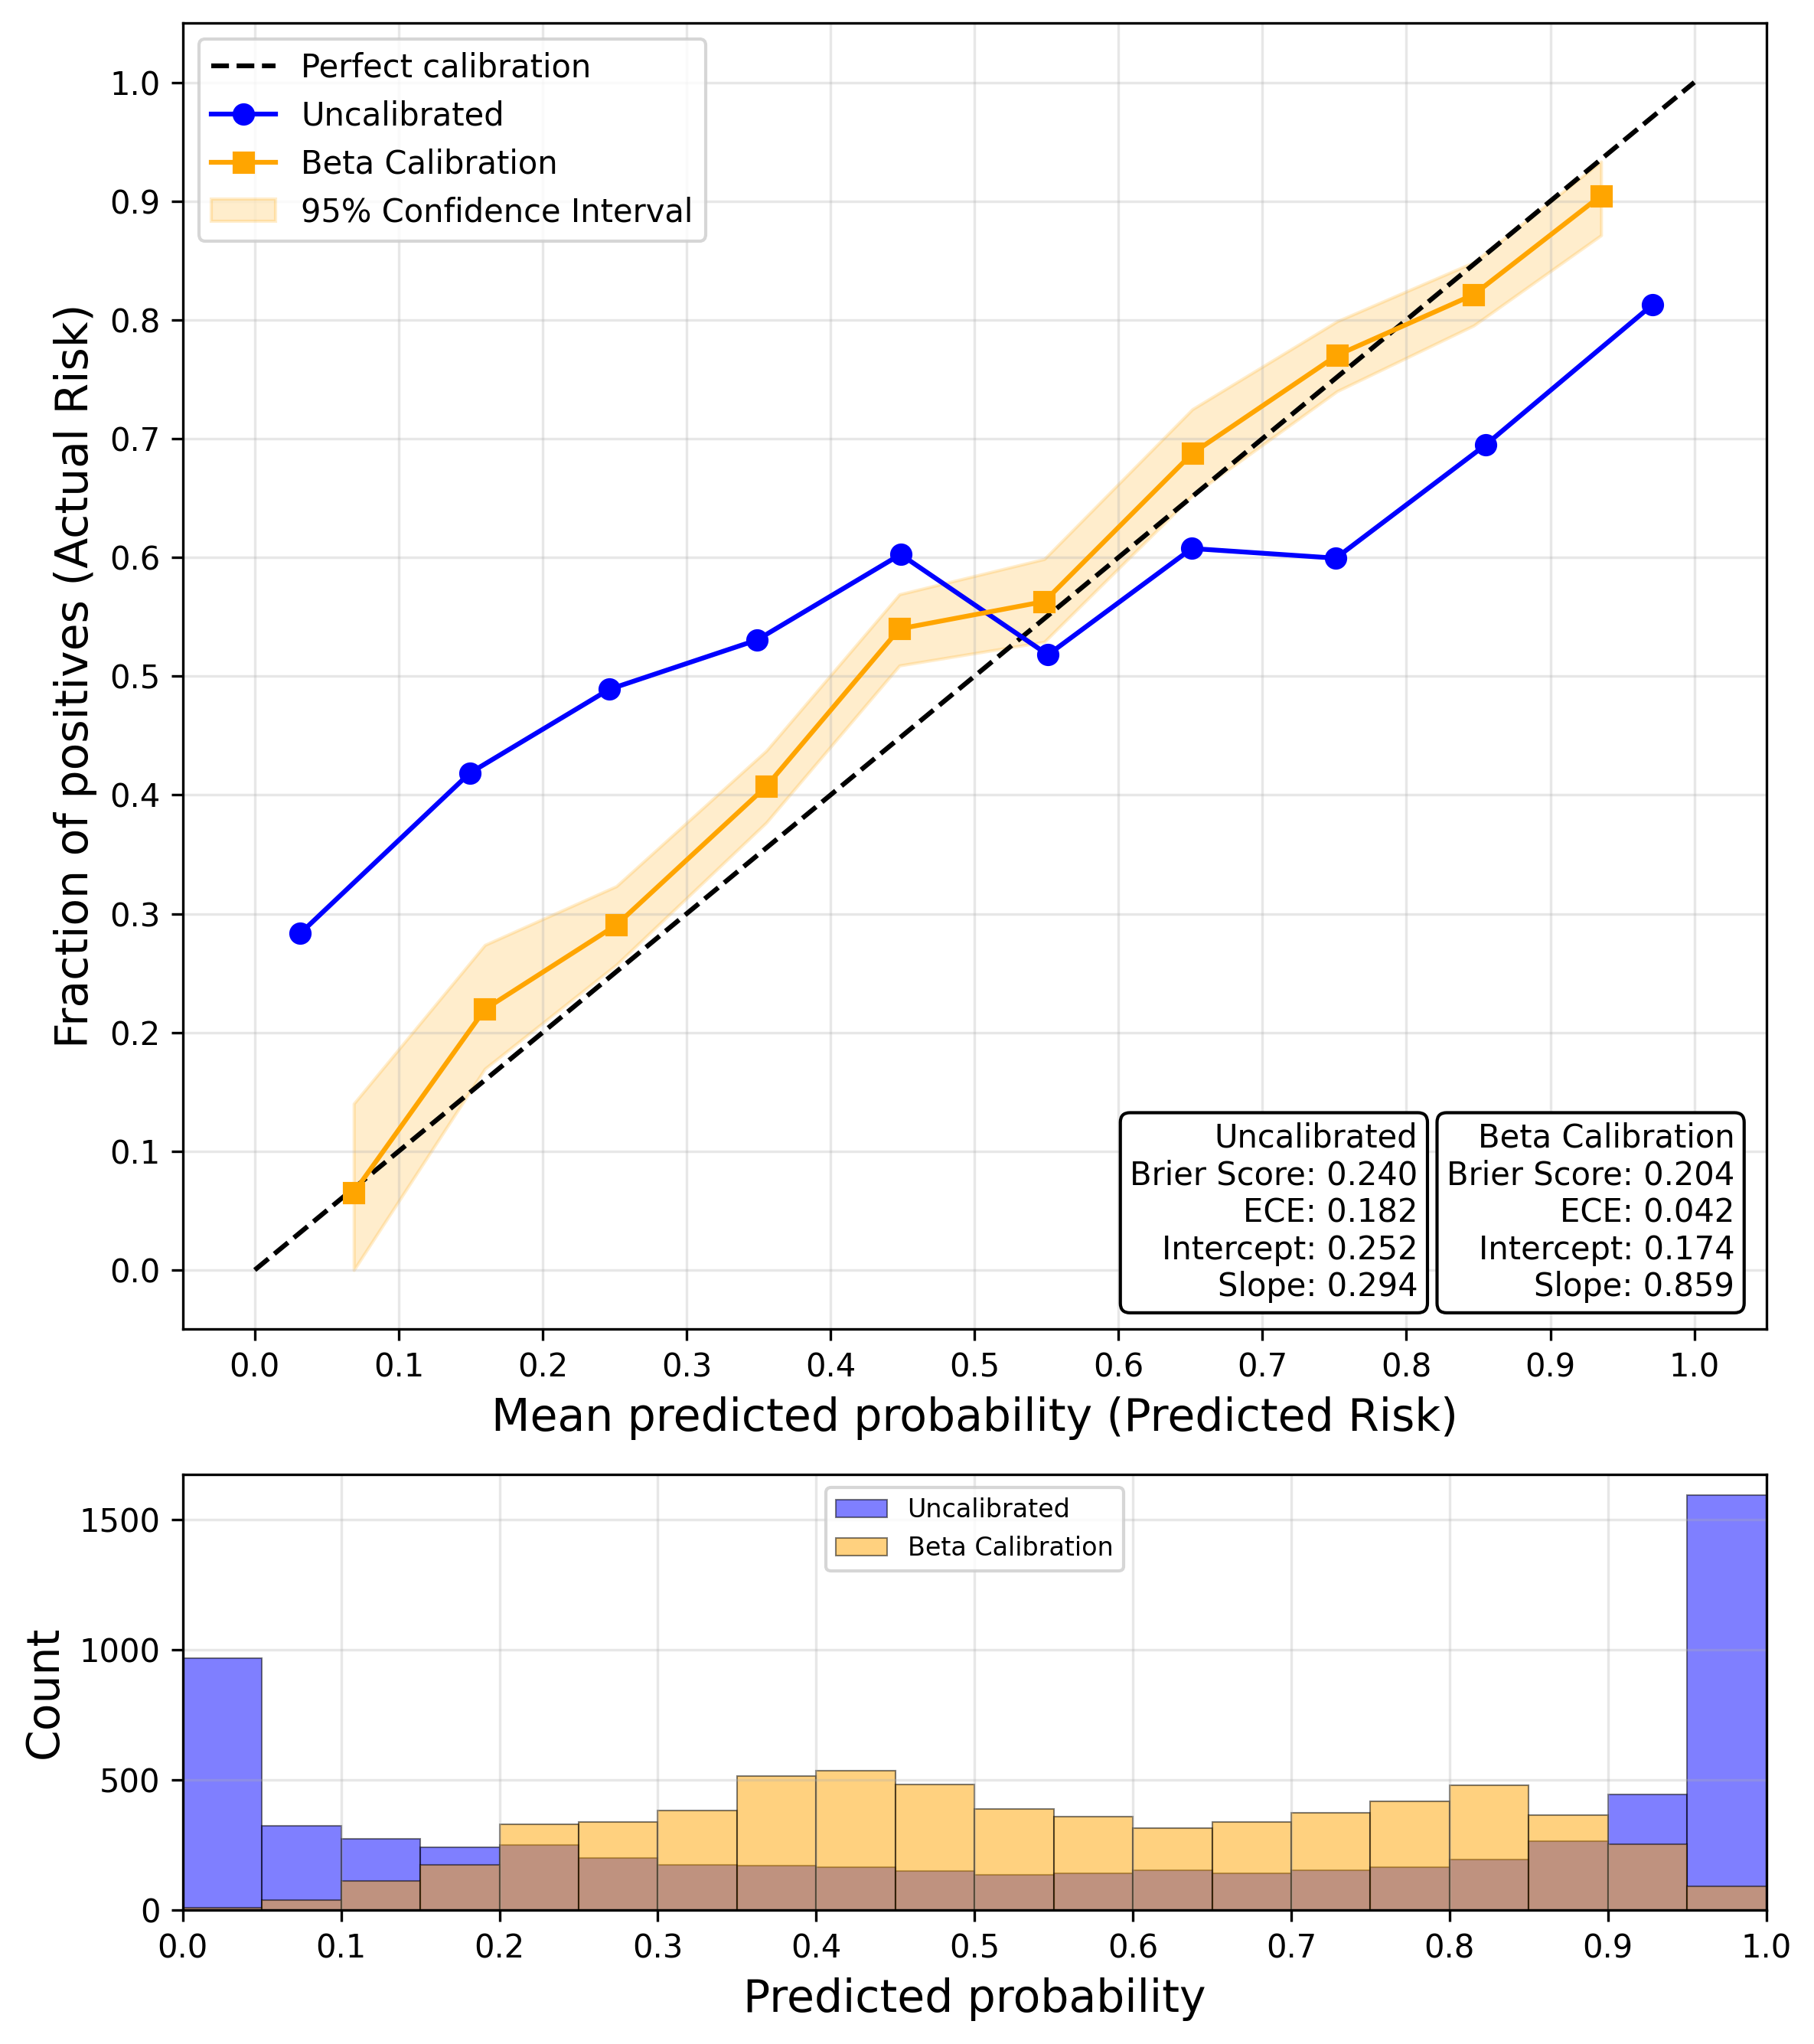
\includegraphics[width=1.0\textwidth]{figures/calibration/type_classification_nacc_test_calibration_curve.png}
    \caption{Model calibration curves of the NACC cross-center validation for the AD vs. non-AD classification task}
    \begin{minipage}{\textwidth}
      \footnotesize \hl{The horizontal axis shows the predicted probability and the vertical axis shows the observed frequency of the positive class. The diagonal line represents perfect calibration, and the curves compare the model before and after beta calibration.}
    \end{minipage}
    \label{fig:ad_nonad_calib_curve}
\end{figure}

The clinical utility of the calibrated LR model for differentiating AD from non-AD dementia was evaluated using DCA. As illustrated in Figure~\ref{fig:ad_nonad_dca}, the model presented a higher net benefit across a wide probability threshold range of 0.13 to 0.91 compared to strategies that classify all subjects as AD or all subjects as non-AD. The net benefit of the model is more pronounced in critical probability thresholds between 0.30 and 0.70. The strong clinical utility of the LR model is supported by the excellent calibration of its predicted probabilities.

\begin{figure}[ht]
    \centering
    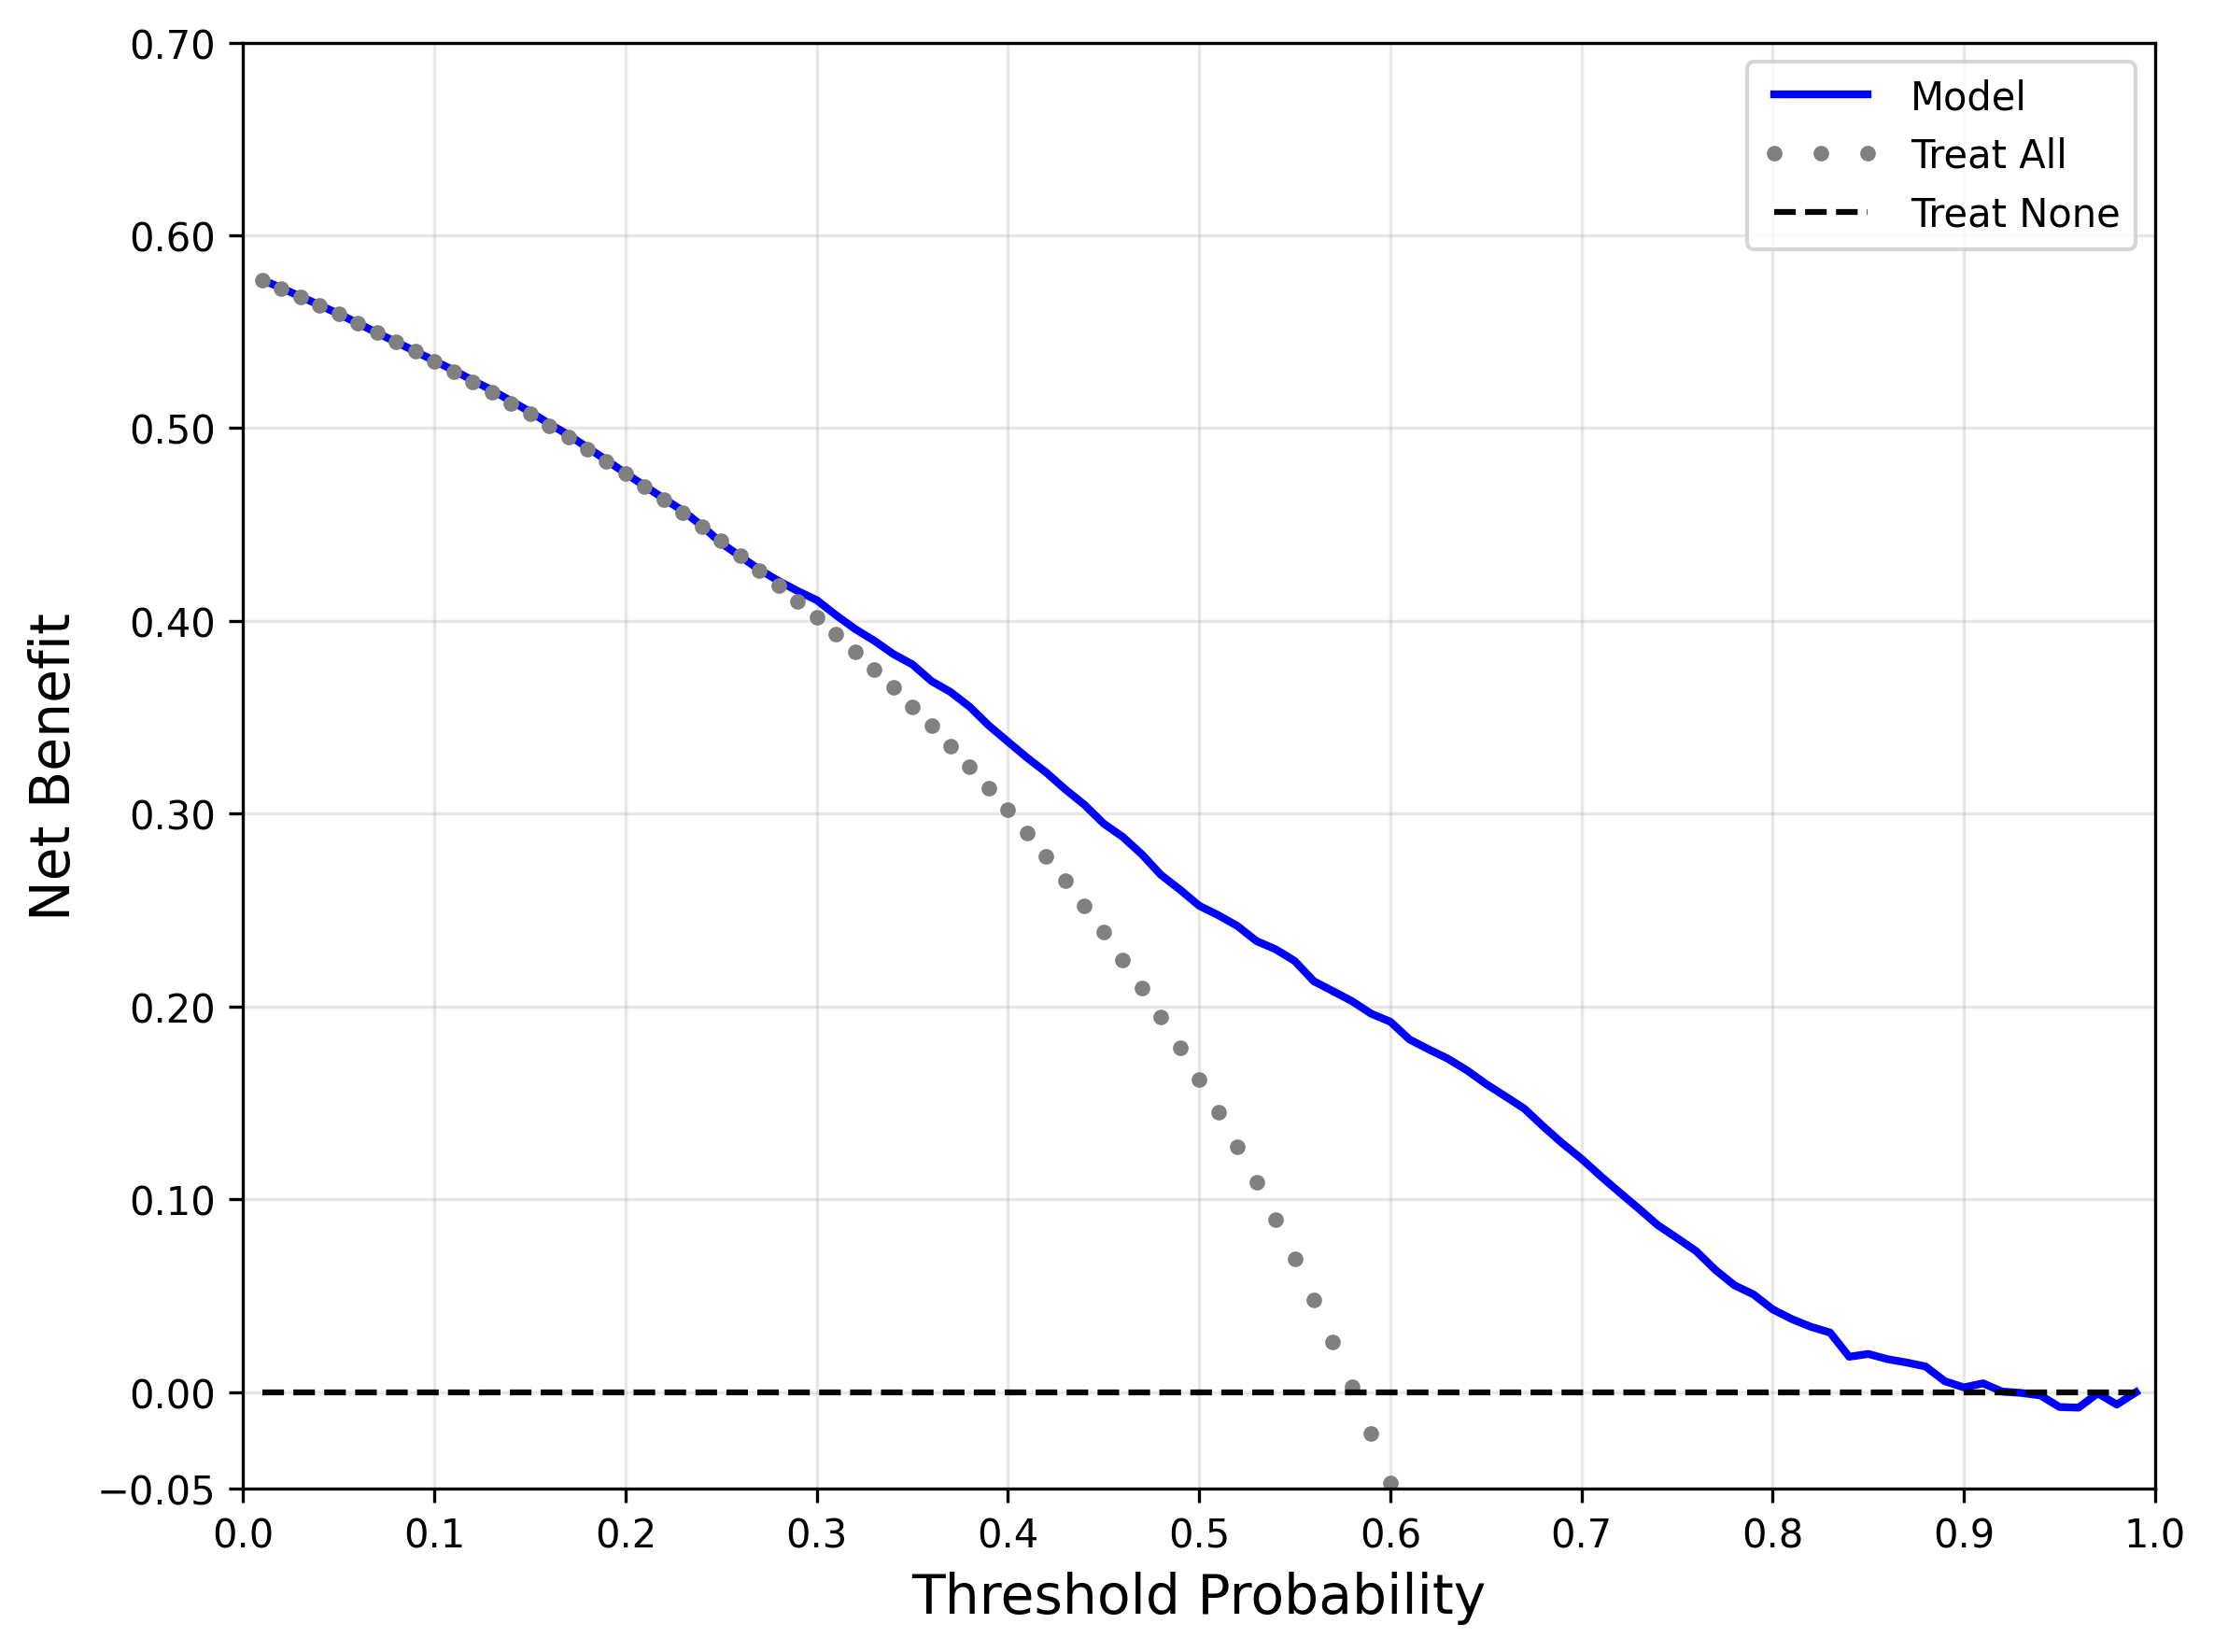
\includegraphics[width=1.0\textwidth]{figures/DCA/type_classification_dca_nacc.png}
    \caption{The decision curve analysis (DCA) of the NACC cross-center validation for the AD vs. non-AD classification task}
    \begin{minipage}{\textwidth}
      \footnotesize "Treat All" refers to the assumption that all subjects are classified as AD, and "Treat None" refers to the assumption that all subjects are classified as non-AD.
    \end{minipage}
    \label{fig:ad_nonad_dca}
\end{figure}

The results of the NACC cross-center validation showed a reasonable level of generalizability, considering the complexity of the task. Although the overall classification accuracy was slightly reduced, the selected LR model presented excellent calibration and clinical utility to classify CI subtypes. Consequently, this result supports the third research objective of developing an accessible and cost-effective model to classify CI subtypes.

\subsection{Model Explainability Results}
The bar chart in Figure~\ref{figure:ad_feature_importance} illustrates the global feature importance ranking for the classification of CI subtypes as AD or non-AD. As expected, the LR model was largely influenced by the features obtained from CDR. Memory impairment (MEMORY) was identified as the most important feature, having a SHAP value that significantly exceeds most of the other features. It was observed that moderate and severe memory impairment mainly associated with AD diagnosis. A similar importance pattern was observed with the impairments in orientation (ORIENT), which was ranked as the second most important feature. It was followed by challenges related to personal care (PERSCARE), but impairments in this domain contributed to the classification of non-AD. Demographic influence was also observed, with age (NACCAGE) ranking as the fourth most critical factor. Older subjects were found to be more likely to be classified as AD. Interestingly, the functional ability to remember dates (REMDATES) played a minimal role in this task, ranking as the second least important feature despite being a top predictor for classifying cognitive decline in the other classification tasks. This indicates that while functional assessments are excellent for classifying cognitive status, clinical ratings (CDR) are more effective for determining the specific etiology (AD vs. non-AD).

\begin{figure}[ht]
    \centering
    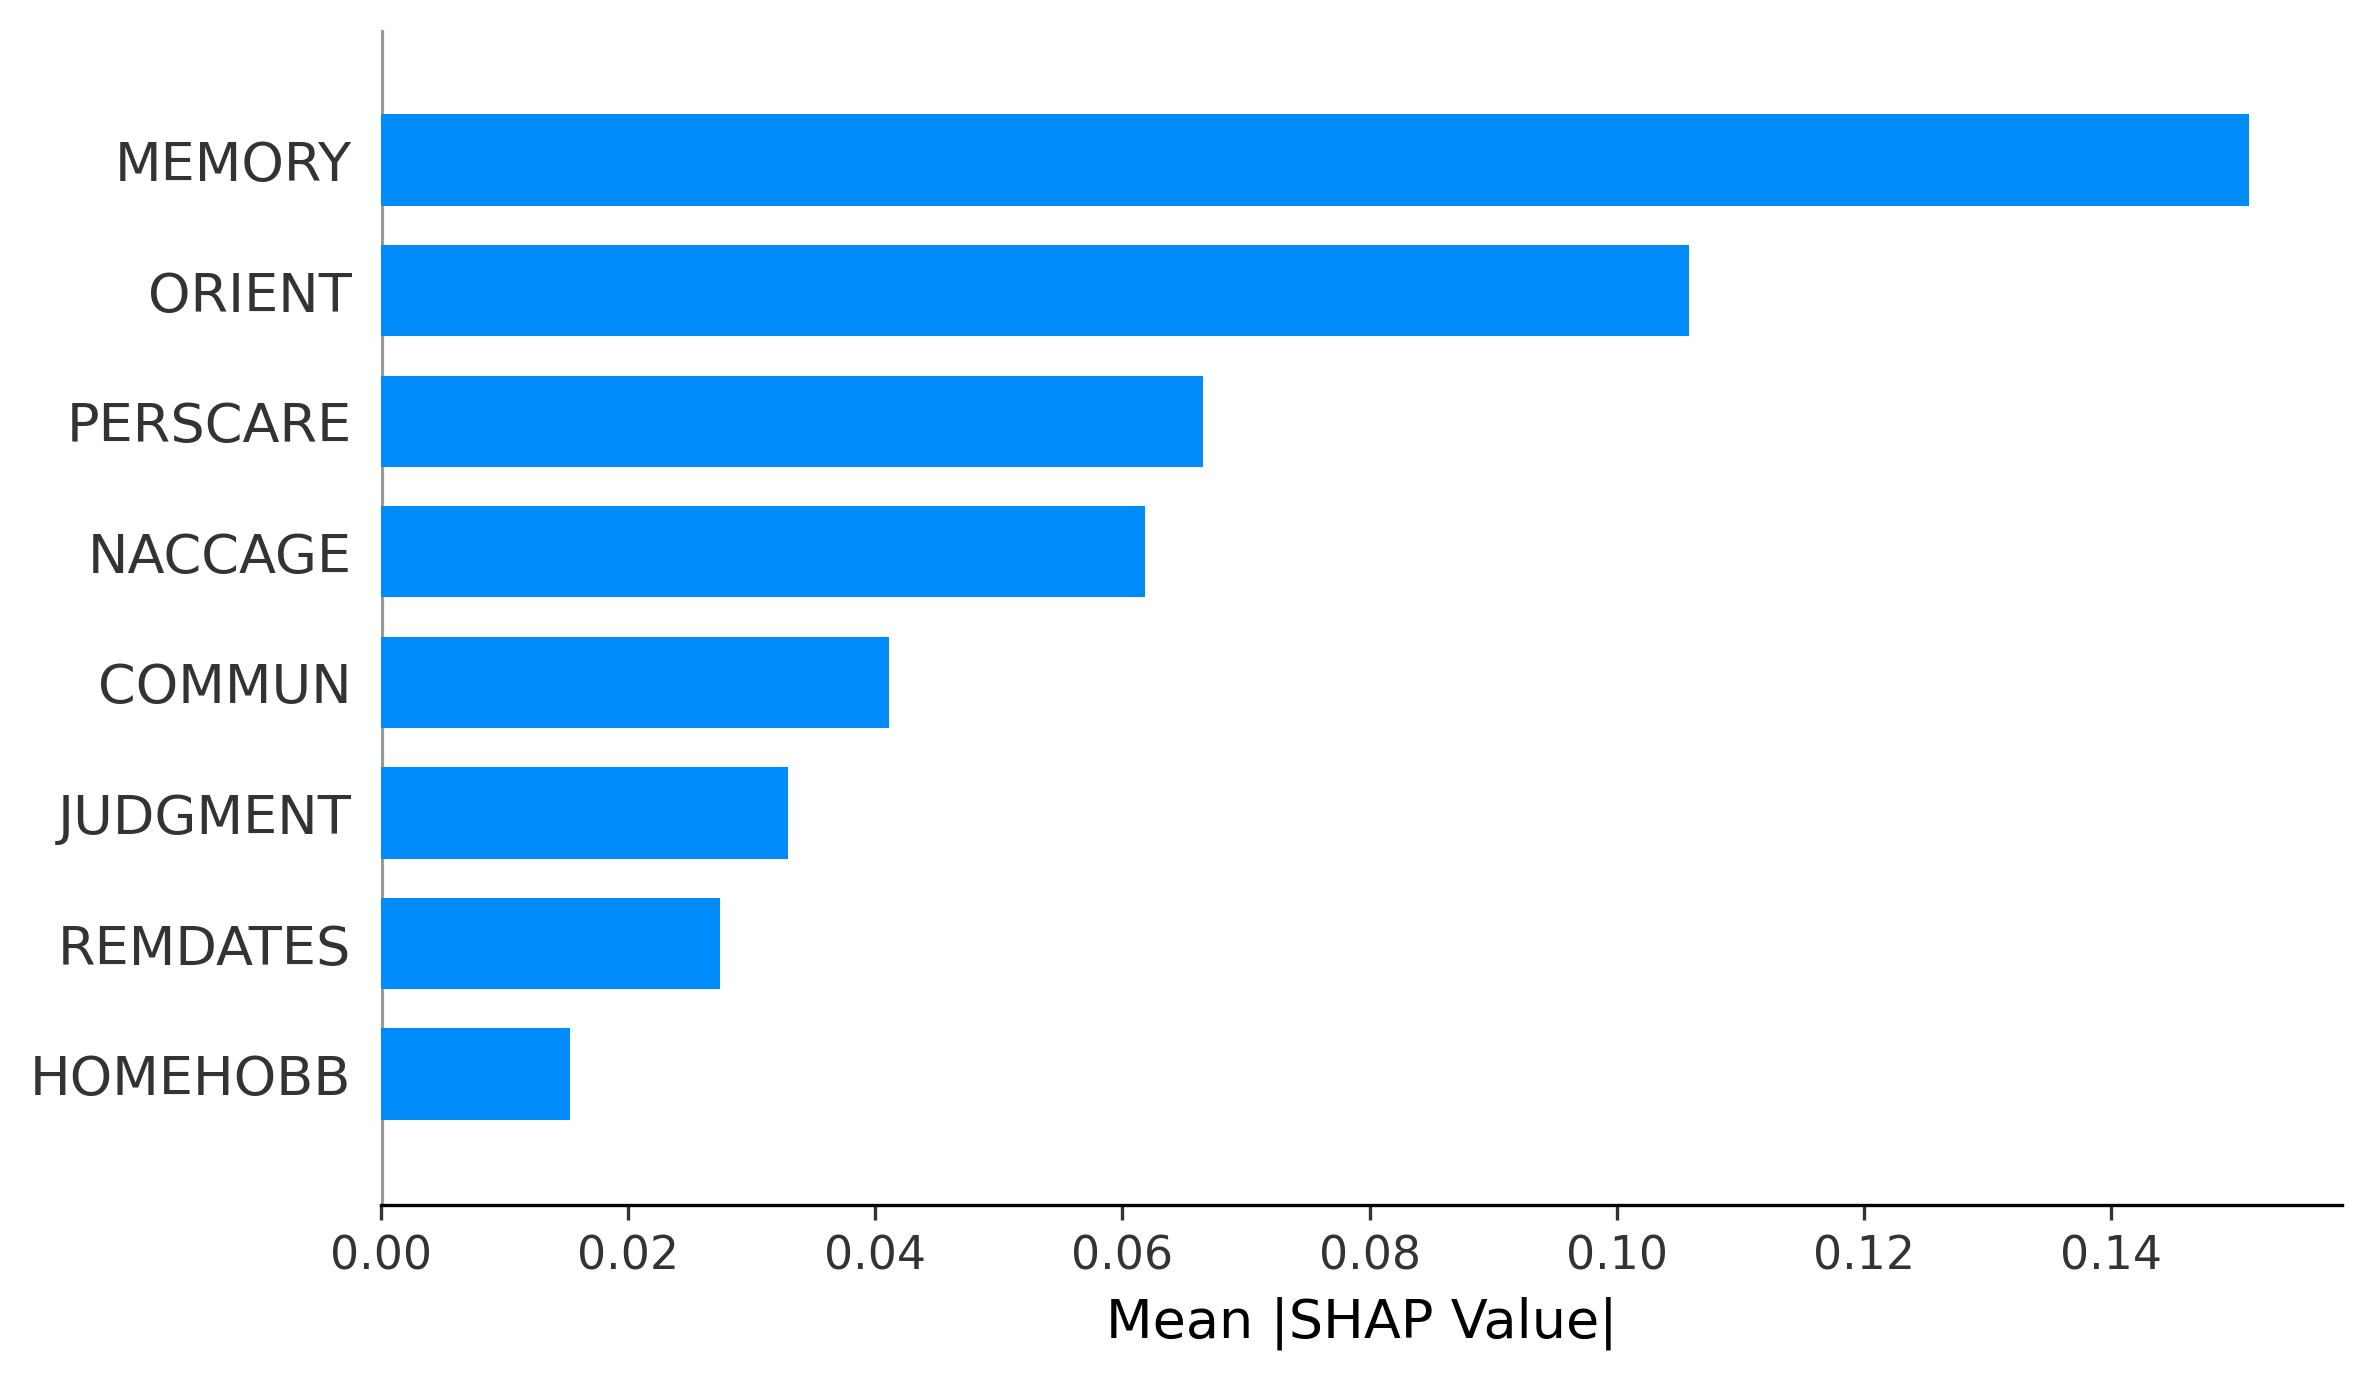
\includegraphics[width=1.0\textwidth]{figures/XAI/type_classification_nacc_shap_barchart.png}
    \caption{Feature importance in the NACC cross-center validation and the ADNI external validation for the AD vs. non-AD classification task}
    \begin{minipage}{\textwidth}
      \footnotesize \hl{The bars represent the mean absolute SHAP value of each feature, which ranks the contribution of the feature to the model prediction in the two validation datasets.}
    \end{minipage}
    \label{figure:ad_feature_importance}
\end{figure}

In this task, a local explanation was performed to evaluate how the features contribute to the model classification at the individual levels. Two correctly classified AD instances were randomly selected for analysis. The influence of features in these two instances is presented by SHAP waterfall plots in Figure~\ref{figure:ad_pos_waterfall}. The instances have different feature values that led to the classification of AD, although both resulted in a probability of 53\%. In Instance B, AD classification was primarily driven by mild impairments in orientation (ORIENT) and memory (MEMORY). In contrast, Instance A's older age combined with preserved ability of personal care (PERSCARE) was sufficient to push the classification towards AD despite questionable impairment in memory.

\begin{figure}[ht]
    \centering
    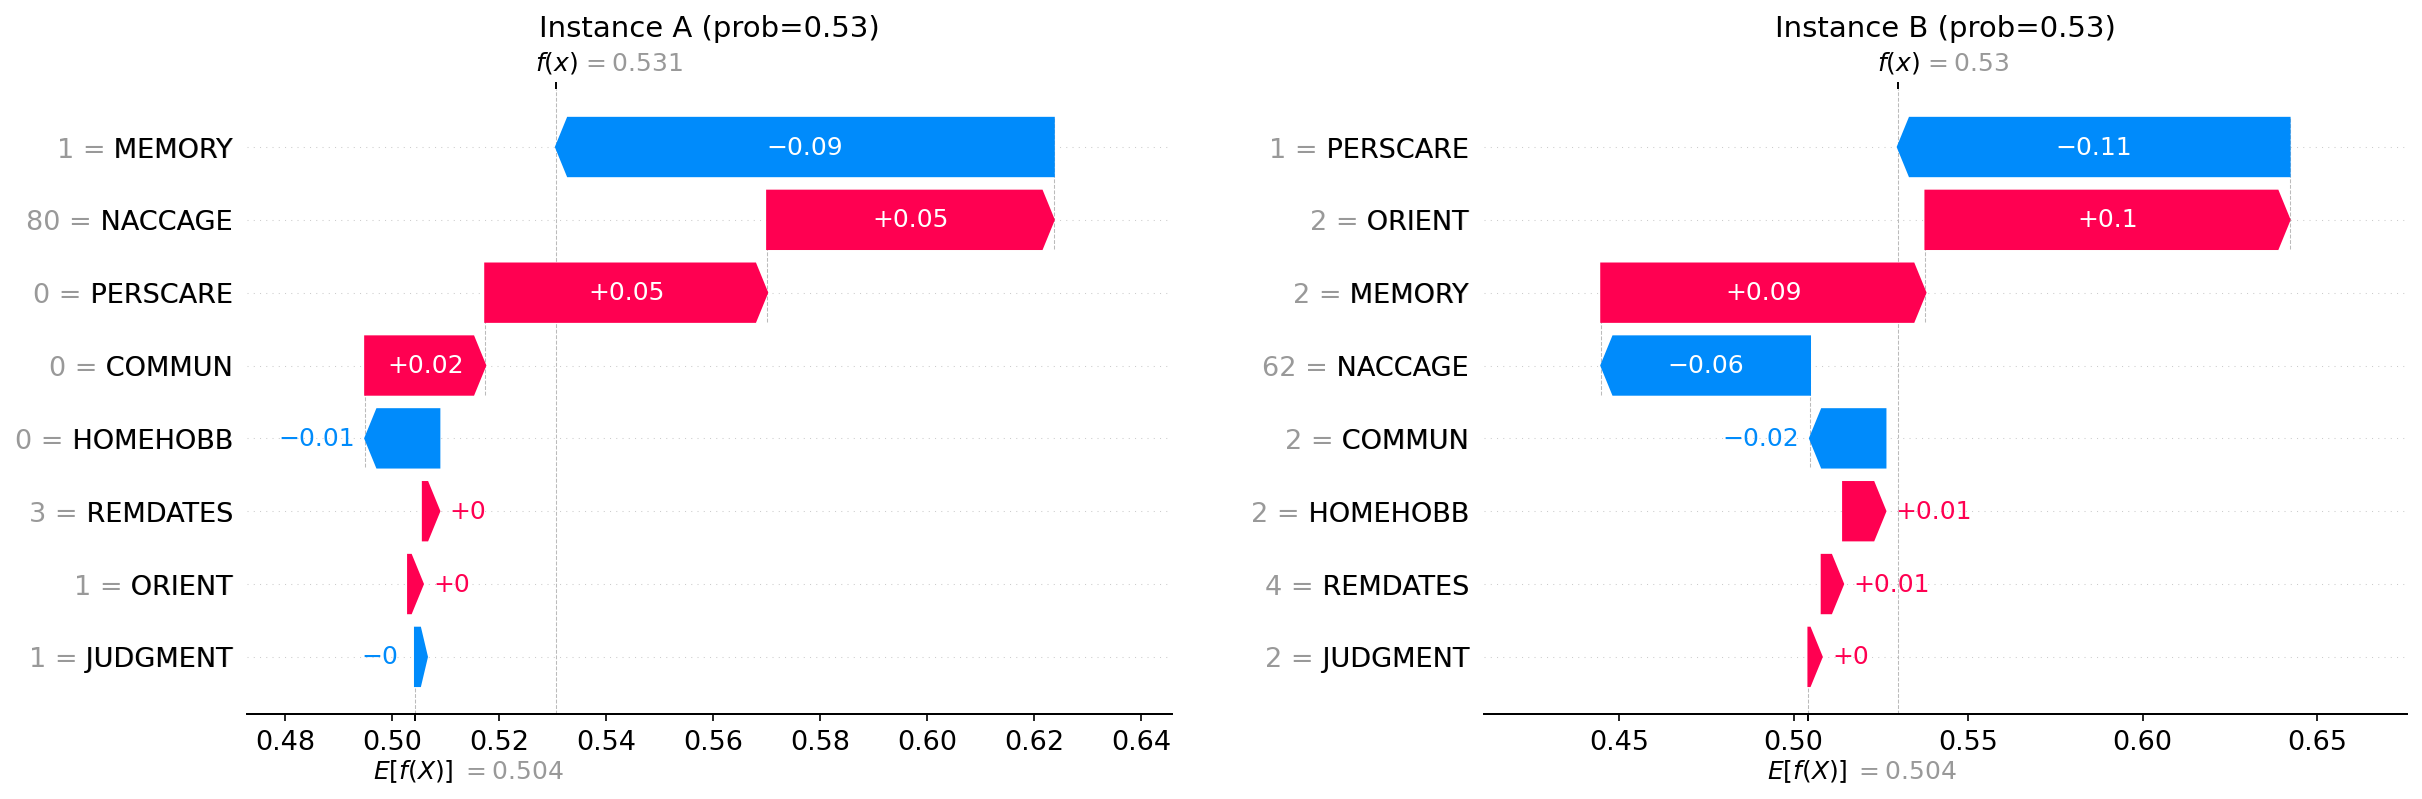
\includegraphics[width=1.0\textwidth]{figures/XAI/type_classification_nacc_true_positive_waterfall.png}
    \caption{SHAP waterfall plots for two instances correctly classified as Alzheimer's disease}
    \begin{minipage}{\textwidth}
      \footnotesize \hl{The plot shows how the value of each feature shifts the prediction from the base value to the final predicted probability for a single instance.}
    \end{minipage}
    \label{figure:ad_pos_waterfall}
\end{figure}

\newpage
A similar analysis was performed with two non-AD instances in Figure~\ref{figure:ad_neg_waterfall}. \textit{Instance A} represents a scenario where the AD indicator of 86 years of age was successfully reversed by preserving key cognitive functions, specifically normal orientation and only questionable memory impairment. \textit{Instance B} presented a different profile. It was classified as non-AD regardless of mild memory impairment. This is due to the questionable ability of personal care despite a relatively younger age. As a side note, it can be observed that features with low global importance have minimal to no influence on the model outcome in the four individually explained instances.

\begin{figure}[ht]
    \centering
    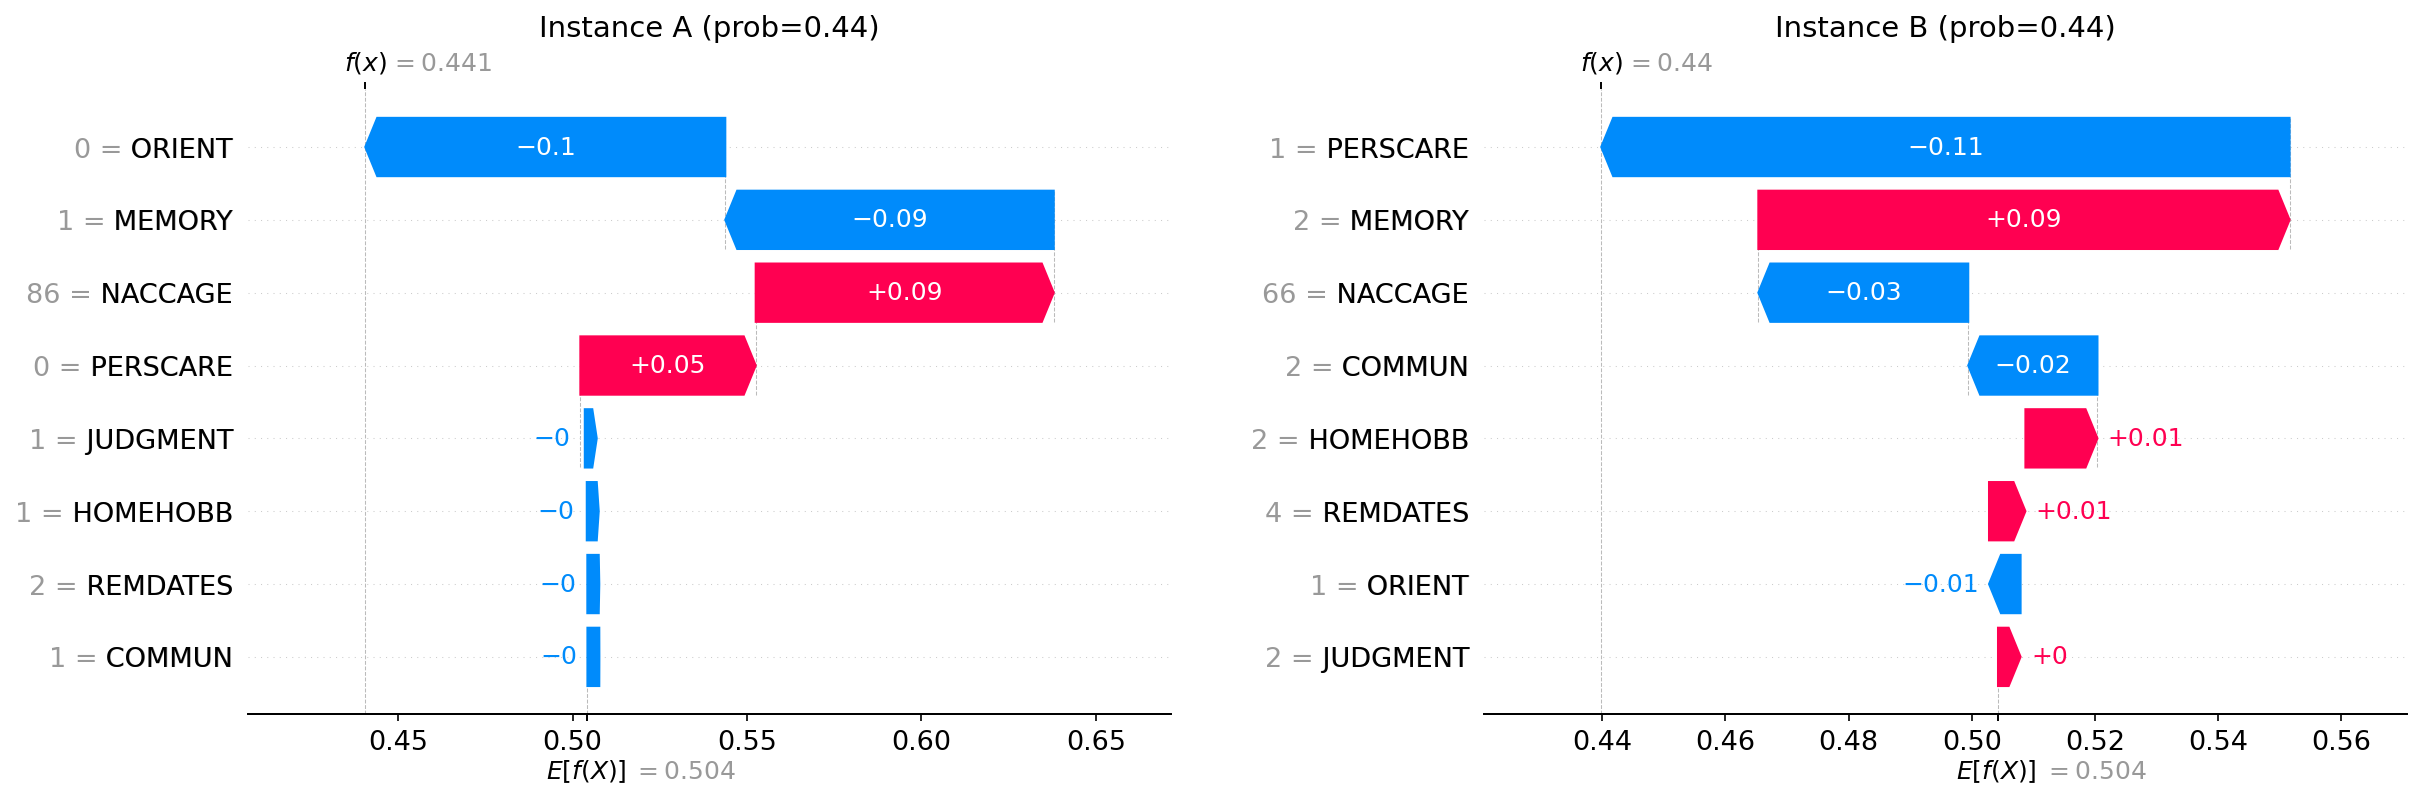
\includegraphics[width=1.0\textwidth]{figures/XAI/type_classification_nacc_true_negative_waterfall.png}
    \caption{SHAP waterfall plots for two instances correctly classified as non Alzheimer's disease}
    \begin{minipage}{\textwidth}
      \footnotesize \hl{The plot shows how the value of each feature shifts the prediction from the base value to the final predicted probability for a single instance.}
    \end{minipage}
    \label{figure:ad_neg_waterfall}
\end{figure}